% This LaTeX document needs to be compiled with XeLaTeX.
\documentclass[10pt]{article}
\usepackage[utf8]{inputenc}
\usepackage{graphicx}
\usepackage[export]{adjustbox}
\graphicspath{ {./images/} }
\usepackage{amsmath}
\usepackage{amsfonts}
\usepackage{amssymb}
\usepackage[version=4]{mhchem}
\usepackage{stmaryrd}
\usepackage{bbold}
\usepackage[fallback]{xeCJK}
\usepackage{polyglossia}
\usepackage{fontspec}
\setCJKmainfont{Noto Serif CJK SC}

\setmainlanguage{english}
\setmainfont{CMU Serif}

%New command to display footnote whose markers will always be hidden
\let\svthefootnote\thefootnote
\newcommand\blfootnotetext[1]{%
  \let\thefootnote\relax\footnote{#1}%
  \addtocounter{footnote}{-1}%
  \let\thefootnote\svthefootnote%
}

%Overriding the \footnotetext command to hide the marker if its value is `0`
\let\svfootnotetext\footnotetext
\renewcommand\footnotetext[2][?]{%
  \if\relax#1\relax%
    \ifnum\value{footnote}=0\blfootnotetext{#2}\else\svfootnotetext{#2}\fi%
  \else%
    \if?#1\ifnum\value{footnote}=0\blfootnotetext{#2}\else\svfootnotetext{#2}\fi%
    \else\svfootnotetext[#1]{#2}\fi%
  \fi
}

\def\Perp{\perp\!\!\!\perp}

\begin{document}
\begin{center}
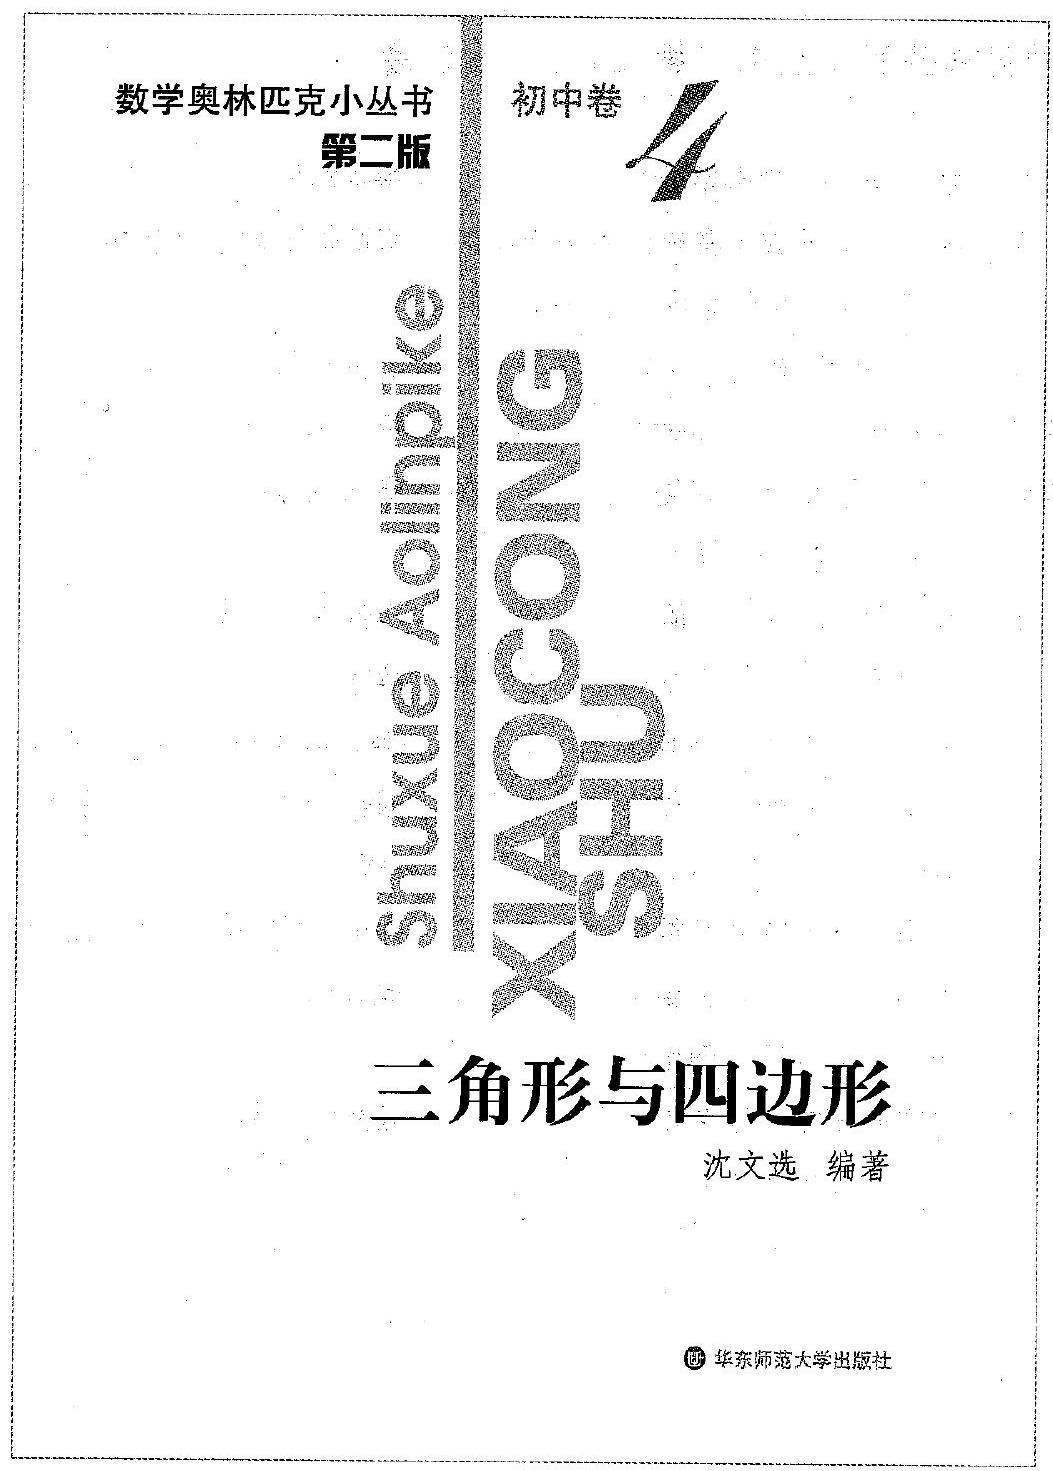
\includegraphics[max width=\textwidth]{2024_10_30_2c8f45efd4a519b08e1ag-001}
\end{center}

\section*{数学奥林匹克小丛书(第二版)编委会}
冯志刚 第53届IMO中国队副领队、上海中学特级教师\\
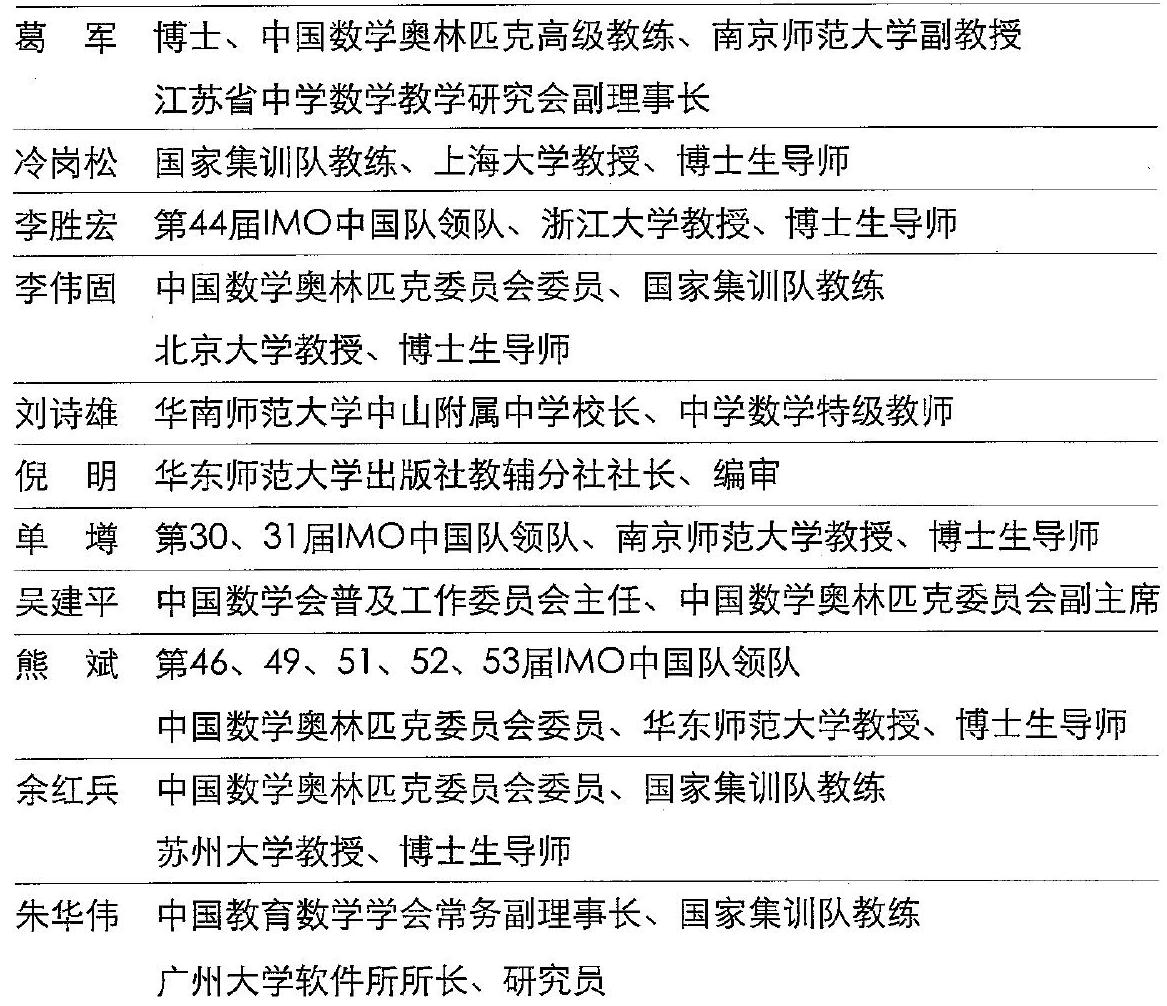
\includegraphics[max width=\textwidth, center]{2024_10_30_2c8f45efd4a519b08e1ag-002}

\section*{总}
\begin{center}
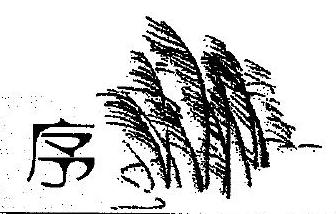
\includegraphics[max width=\textwidth]{2024_10_30_2c8f45efd4a519b08e1ag-003}
\end{center}

数学竟赛像其他竞赛活动一样,是青少年学生的一种智力竞赛。在类似的以基础科学为竞赛内容的智力竞赛活动中,数学竞赛的历史最悠久、国际性强,影响也最大。我国于1956年开始举行数学竞赛,当时最有威望的著名数学家华罗庚、苏步青、江泽涵等都积极参加领导和组织竟赛活动,并组织出版了一系列青少年数学读物,激励了一大批青年学生立志从事科学事业。我国于1986年起参加国际数学奥林匹克,多次获得团体总分第一,并于1990年在北京成功地举办了第 31 届国际数学奥林匹克,这标志着我国数学竞赛水平在国际上居领先地位,为各国科学家与教育家所瞩目。

我国数学竞赛活动表明,凡是开展好的地区和单位,都能大大激发学生的学习数学的兴趣,有利于培养创造性思维,提高学生的学习效率。这项竟赛活动,将健康的竞争机制引进数学教学过程中,有利于选拔人才。由数学竞赛选拔的优胜者,既有踏实广泛的数学基础,又有刻苦钻研、科学的学习方法,其中的不少青年学生将来会成为出色的科学工作者。在美国,数学竟赛的优胜者中后来成名如米尔诺(J. W. Milnor)、芒福德(D. B. Mumford)、奎伦 (D. Quillen)等都是菲尔兹数学奖的获得者;在波兰,著名数论专家辛哲尔 (A. Schinzel)学生时代是一位数学竟赛优胜者;在匈牙利,著名数学家费叶尔 (L. Fejér)、里斯(M. Riesz)、舍贵(G. Szegö)、哈尔(A. Haar)、拉多 (T. Radó)等都曾是数学竞赛获奖者。匈牙利是开展数学竟赛活动最早的国家,产生了同它的人口不成比例的许多大数学家!

在开展数学竞赛的活动同时,各学校能加强联系,彼此交流数学教学经验,从这种意义上来说,数学竟赛可能成为数学课程改革的"催化剂",成为培养优秀人才的有力措施。

不过,应当注意在数学竟赛活动中,注意普及与提高相结合,而且要以普及为主,使竞赛具有广泛的群众基础,否则难以持久。

当然,现在有些人过于关注数学竞赛的成绩,组织和参与都具有很强的功利目的,过分扩大数学竟赛的作用,这些都是不正确的,违背了开展数学竞赛活动的本意。这些缺点有其深层次的社会原因,需要逐步加以克服,不必因

\section*{001}
为有某些缺点,就否定这项活动。\\
我十分高兴看到这套《数学奥林匹克小丛书》的正式出版。这套书,规模大、专题细。据我所知,这样的丛书还不多见。这套书不仅对数学竟赛中出现的常用方法作了阐述,而且对竞赛题作了精到的分析解答,不少出自作者自已的研究所得,是一套很好的数学竞赛专题教程,也是中小学生和教师的参考书。

这套小丛书的作者都是数学竟赛教学和研究人员,不少是国家集训队的教练和国家队的领队。他们为我国开展数学竞赛的活动和我国学生在 IMO上取得成绩、为国争光作出了贡献,为这套书尽早面世付出了艰辛的劳动。华东师大出版社在出版《奥数教程》和《走向 IMO》等竞赛图书基础上,策划组织了这套丛书,花了不少心血。我非常感谢作者们和编辑们在这方面所做的工作,并衷心祝愿我国的数学竟赛活动开展得越来越好。

\section*{五光}
\footnotetext{王元,著名数学家,中国科学院院士,曾任中国数学会理事长、中国数学奥林匹克委员会主席.
}\section*{夏门郑剑雄高中数学竞赛系列}
全国小学奥数群:221739457,全国初中奥数学生群:253736211,全国高中奥数学生群591782992全国初中奥数教练群112464128,全国高中奥数教练群195949359竞赛公众号:新浪微博@郑剑雄 微信:v136257437 QQ:136257437\\
业务:初高中联赛班、培优班、美国高中数学、教师培训、机构教学产品研发、讲义资料出售等\\
1 三角形的基本概念和性质 ..... 001\\
2 三角形的面积、边角间关系定理 ..... 008\\
3 全等三角形 ..... 018\\
4 相似三角形 ..... 030\\
5 三角形中与比例线段有关的几个定理 ..... 040\\
6 三角形的四心 ..... 050\\
7 三角形的内接三角形 ..... 069\\
8 直角三角形 ..... 074\\
9 等腰三角形 ..... 083\\
10 等边三角形 ..... 089\\
11 四边形的基本概念与性质 ..... 095\\
12 平行四边形 ..... 103\\
13 矩形与菱形 ..... 113\\
14 正方形 ..... 121\\
15 梯形 ..... 131\\
16 圆内接四边形与圆外切四边形 ..... 140\\
习题解答 ..... 149\\
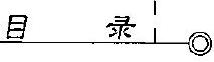
\includegraphics[max width=\textwidth, center]{2024_10_30_2c8f45efd4a519b08e1ag-005}

全国小学奥数群:221739457,全国初中奥数学生群:253736211,全国高中奥数学生群591782992全国初中奥数教练群112464128,全国高中奥数教练群195949359竞赛公众号:新浪微博@郑剑雄 微信:v136257437 QQ:136257437\\
业务:初高中联赛班、培优班、美国高中数学、教师培训、机构教学产品研发、讲义资料出售等

每个三角形都有三条边和三个角,它们是互相联系、互相制约的,这体现在以下方面:\\
(1) 边与边之间的关系:两边之和大于第三边,两边之差小于第三边。\\
(2)角与角之间的关系:三个内角的和等于 $180^{\circ}$ ,即在 $\triangle A B C$ 中有 $\angle A+\angle B+\angle C=180^{\circ}$ 。由此即知三角形的一个外角等于与它不相邻的两个内角之和。

三角形的角平分线 三角形一个角的平分线与这个角的对边相交,这个角的顶点和交点之间的线段叫做三角形的角平分线。

三角形的中线 在三角形中,连结一个顶点和它的对边中点的线段叫做三角形的中线。

三角形的高 从三角形一个顶点向它的对边所在直线画垂线,顶点和垂足间的线段叫做三角形的高线,简称三角形的高。

三角形的中位线 连结三角形两边中点的线段叫做三角形的中位线。中位线平行于第三边且等于第三边的一半。

三角形的外角平分线 三角形一个内角的邻补角的平分线与这个角的对边的延长线相交,这个角的顶点和交点之间的线段叫做三角形的外角平分线。

三角形的内角平分线上的点到这个角的两边的距离相等。同一个三角形中,大角的角平分线短于小角的角平分线。

三角形中任何一边上的中线都把三角形分成面积相等的两部分。同一个三角形中,大边上的中线短于小边上的中线。

三角形的任何一边上的高都垂直于该边. 三角形的三条高未必都在三角形的内部。

三角形的内角平分线、中线和高又有相同之处:在同一个三角形中,无论是三条中线,还是三条高,或者三条内角平分线,它们分别相交于一点。

三角形顶角的平分线与底边上的高所夹的角等于两底角差的一半。\\
事实上,如图 1-1, $A T$ 为 $\angle B A C$ 的平分线, $A H$为 $B C$ 边上的高,令 $\angle T A H$ 为 $\theta$ ,则 $2 \theta=(\angle B A H-$ $\angle B A T)+(\angle C A T-\angle C A H)=\angle B A H-\angle C A H=$ $\left(90^{\circ}-\angle B\right)-\left(90^{\circ}-\angle C\right)=\angle C-\angle B$.

在不混淆的情况下,有时,三角形的角平分线、中线\\
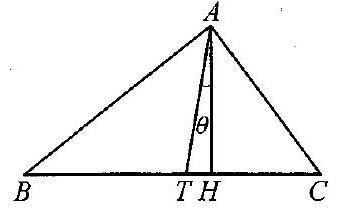
\includegraphics[max width=\textwidth, center]{2024_10_30_2c8f45efd4a519b08e1ag-008}

图1-1

和高也指它们所在的直线。

例1 点 $C_{1} 、 A_{1} 、 B_{1}$ 分别在 $\triangle A B C$ 的边 $A B 、 B C$ 和 $C A$ 上, 且满足 $A C_{1}: C_{1} B=B A_{1}: A_{1} C=C B_{1}: B_{1} A=1: 3$. 求证: $\triangle A B C$ 的周长 $p$ 与 $\triangle A_{1} B_{1} C_{1}$ 的周长 $p^{\prime}$ 之间有不等式:

\begin{align*}
\frac{1}{2} p<p^{\prime}<\frac{3}{4} p
\end{align*}

(第15届全俄奥林匹克题)\\
证明 如图 1-2,注意到三角形两边之差小于第三边,故有

\begin{align*}
\begin{aligned}
& A_{1} C-C B_{1}<A_{1} B_{1} \\
& B_{1} A-A C_{1}<B_{1} C_{1} \\
& C_{1} B-B A_{1}<C_{1} A_{1}
\end{aligned}
\end{align*}

设 $B C=a, C A=b, A B=c, B_{1} C_{1}=a_{1}$, $C_{1} A_{1}=b_{1}, A_{1} B_{1}=c_{1}$ ,则

\begin{align*}
\begin{aligned}
& \frac{3}{4} a-\frac{1}{4} b<c_{1}, \\
& \frac{3}{4} b-\frac{1}{4} c<a_{1} \\
& \frac{3}{4} c-\frac{1}{4} a<b_{1} .
\end{aligned}
\end{align*}

\begin{center}
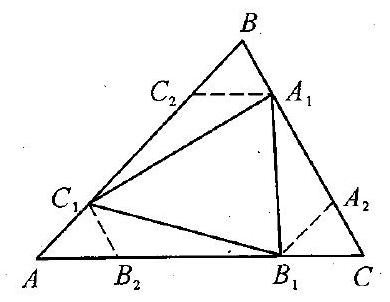
\includegraphics[max width=\textwidth]{2024_10_30_2c8f45efd4a519b08e1ag-008(1)}
\end{center}

图1-2

三式相加,得

\begin{align*}
\frac{1}{2}(a+b+c)<a_{1}+b_{1}+c_{1}
\end{align*}

即

\begin{align*}
\frac{1}{2} p<p^{\prime}
\end{align*}

再在 $\triangle A B C$ 各边上截取 $A_{1} A_{2}=\frac{1}{2} a, B_{1} B_{2}=\frac{1}{2} b, C_{1} C_{2}=\frac{1}{2} c$, 易证

\begin{align*}
A_{2} B_{1}=\frac{1}{4} c, B_{2} C_{1}=\frac{1}{4} a, C_{2} A_{1}=\frac{1}{4} b .
\end{align*}

\section*{厦门郑剑雄高中数学竞赛系列}
全国小学奥数群:221739457,全国初中奥数学生群:253736211,全国高中奥数学生群591782992全国初中奥数教练群112464128,全国高中奥数教练群195949359竞赛公众号:新浪微博@郑剑雄 微信:v136257437 QQ:136257437\\
业务:初高中联赛班、培优班、美国高中数学、教师培训、机构教学产品研发、讲义资料出售等

又注意到三角形两边之和大于第三边,有

\begin{align*}
\frac{2}{4} a+\frac{1}{4} c>c_{1}, \frac{2}{4} b+\frac{1}{4} a>a_{1}, \frac{2}{4} c+\frac{1}{4} b>b_{1} .
\end{align*}

三式相加,得

\begin{align*}
\frac{3}{4}(a+b+c)>a_{1}+b_{1}+c_{1}
\end{align*}

即

\begin{align*}
p^{\prime}<\frac{3}{4} p
\end{align*}

故

\begin{align*}
\frac{1}{2} p<p^{\prime}<\frac{3}{4} p
\end{align*}

例2 如图 $1-3, \angle 1+\angle 2+\angle 3+\angle 4+\angle 5+\angle 6+\angle 7$ 的度数为 ( )。\\
A. $450^{\circ}$\\
B. $540^{\circ}$\\
C. $630^{\circ}$\\
D. $720^{\circ}$\\
(1997 年安徽部分地市联赛题)\\
解 选 B. 理由:记 $\angle 1 、 \angle 2 、 \angle 3 、 \angle 4$ 、 $\angle 5 、 \angle 6 、 \angle 7$ 的顶点分别为 $A 、 B 、 C 、 D 、 E$ 、 $F 、 G$ ,设 $A E$ 交 $B G$ 于 $M, A D$ 交 $B G$ 于 $N$ 。记 $\angle E M N=\angle 8, \angle D N M=\alpha$ ,则\\
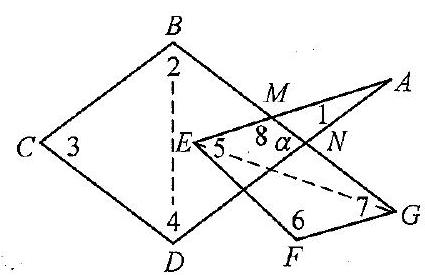
\includegraphics[max width=\textwidth, center]{2024_10_30_2c8f45efd4a519b08e1ag-009}

图1-3

\begin{align*}
\alpha=180^{\circ}-\angle M N A=180^{\circ}-\angle 8+\angle 1
\end{align*}

即

\begin{align*}
\alpha+\angle 8-\angle 1=180^{\circ}
\end{align*}

连 $B D 、 E G$ ,则

\begin{align*}
\begin{aligned}
& \angle 2+\angle 3+\angle 4+\alpha=360^{\circ} \\
& \angle 5+\angle 6+\angle 7+\angle 8=360^{\circ}
\end{aligned}
\end{align*}

从而

\begin{align*}
\begin{aligned}
& \angle 1+\angle 2+\angle 3+\angle 4+\angle 5+\angle 6+\angle 7 \\
= & \angle 1+(\angle 2+\angle 3+\angle 4)+(\angle 5+\angle 6+\angle 7) \\
= & \angle 1+\left(360^{\circ}-\alpha\right)+\left(360^{\circ}-\angle 8\right) \\
= & 720^{\circ}-(\alpha+\angle 8-\angle 1) \\
= & 720^{\circ}-180^{\circ}=540^{\circ} .
\end{aligned}
\end{align*}

例3 在 $\triangle A B C$ 中, $\angle B$ 的平分线与 $\angle C$ 的外角平分线相交于点 $D$. 如果 $\angle A=27^{\circ}$, 那么, $\angle B D C=$ $\qquad$。(2002 年"我爱数学"夏令营竞赛题)\\
解 填 $13.5^{\circ}$ 。理由:如图1-4,因为 $\angle A=27^{\circ} , \angle B C E=\frac{1}{2}(\angle A+$\\
1 三角形的基本概冷和性质\\
$\angle A B C$ ), 则

\begin{align*}
\begin{aligned}
& \angle B D C=\angle B C E-\angle C B D \\
= & \frac{1}{2}(\angle A+\angle A B C)-\frac{1}{2} \angle A B C \\
= & \frac{1}{2} \angle A=13.5^{\circ} .
\end{aligned}
\end{align*}

例 4 如图 $1-5, A A^{\prime} 、 B B^{\prime}$ 分别是 $\angle E A B$ 、 $\angle D B C$ 的平分线。若 $A A^{\prime}=B B^{\prime}=A B$ ,则 $\angle B A C$ 的\\
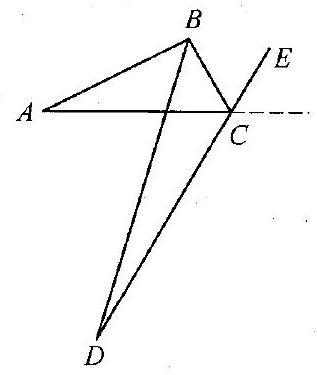
\includegraphics[max width=\textwidth, center]{2024_10_30_2c8f45efd4a519b08e1ag-010(3)}

图1-4

度数为 $\qquad$。(2003 年全国联赛题)\\
解 填 $12^{\circ}$ 。理由:设 $\angle B A C$ 的度数为 $x$ 。\\
因 $A B=B B^{\prime}$ ,故 $\angle B^{\prime} B D=2 x, \angle C B D=$ $4 x$. 又 $A B=A A^{\prime}$, 则\\
$\angle A A^{\prime} B=\angle A B A^{\prime}=\angle C B D=4 x$.\\
因为 $\angle A^{\prime} A B=\frac{1}{2}\left(180^{\circ}-x\right)$, 故\\
$\frac{1}{2}\left(180^{\circ}-x\right)+4 x+4 x=180^{\circ}$.\\
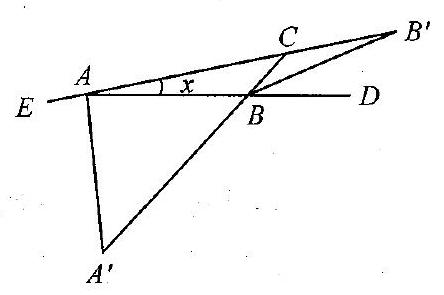
\includegraphics[max width=\textwidth, center]{2024_10_30_2c8f45efd4a519b08e1ag-010(1)}

图1-5

解得

\begin{align*}
x=12^{\circ}
\end{align*}

例 $5 \triangle A B C$ 的边 $A B$ 和 $B C$ 上的高线(分别)不短于边长,试求该三角形的各个角度数。(第 27 届莫斯科奥林匹克题)

解 如图 1-6,设 $A D 、 C E$ 分别是 $B C$ 和 $A B$ 上的高线,则

\begin{align*}
A D \leqslant A B, C E \leqslant B C
\end{align*}

但由题设,知

\begin{align*}
A D \geqslant B C, C E \geqslant A B
\end{align*}

所以

\begin{align*}
A D=A B=C E=C B
\end{align*}

从而 $D 、 B 、 E$ 重合. 如图 1-7.\\
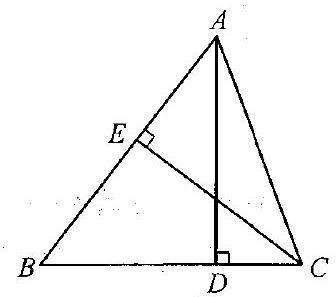
\includegraphics[max width=\textwidth, center]{2024_10_30_2c8f45efd4a519b08e1ag-010}

图1-6\\
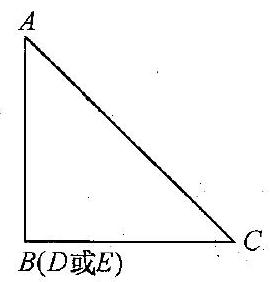
\includegraphics[max width=\textwidth, center]{2024_10_30_2c8f45efd4a519b08e1ag-010(2)}

图1-7

所以 $\triangle A B C$ 是以 $\angle B$ 为直角的等腰直角三角形,因此

\begin{align*}
\angle B=90^{\circ}, \angle A=\angle C=45^{\circ} .
\end{align*}

例6 如图 1-8, $A D$ 是 $\triangle A B C$ 的中线, $E$ 是 $A D$ 上的一点, 且 $A E=$ $\frac{1}{3} A D, C E$ 交 $A B$ 于点 $F$. 若 $A F=1.2 \mathrm{~cm}$, 则 $A B=$ $\qquad$ cm. (2000 年山东省竞赛题)

解 填 6. 理由:过点 $D$ 作 $D G \cdot / / C F$ 交 $A B$ 于 $G$ ,则

即

\begin{align*}
\begin{align*}
& \frac{B G}{G F}=\frac{B D}{D C}=1 \\
& B G=G F
\end{align*} \tag{1}
\end{align*}

又由 $G D / / F E$ ,有

\begin{align*}
\frac{A F}{F G}=\frac{A E}{E D}=\frac{1}{2} \tag{2}
\end{align*}

由此, 即求得 $F G=2.4 \mathrm{~cm}$, 故 $A B=6 \mathrm{~cm}$.\\
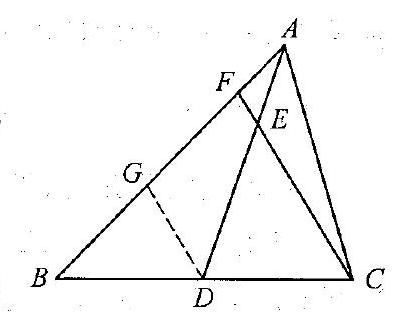
\includegraphics[max width=\textwidth, center]{2024_10_30_2c8f45efd4a519b08e1ag-011(1)}

图1-8

注 此例可以推广,设 $D$ 为 $B C$ 边上一点,且 $B D: D C=\lambda, E$ 是 $A D$ 上一点,且 $A E=\frac{1}{n} A D$ ,按此例求解方法,式(1)(2)分别变为

所以

\begin{align*}
\begin{aligned}
& B G=\lambda G F, \\
& F G=(n-1) A F, \\
A B= & {[(n-1)(\lambda+1)+1] A F }
\end{aligned}
\end{align*}

例7 在 $\triangle A B C$ 中, $P 、 Q$ 分别是边 $A B$ 和 $A C$ 上的点, 中线 $A M$ 与 $P Q$交于 $N$ 。若 $A B: A P=5: 2, A C: A Q=4: 3$, 则 $A M: A N=$ $\qquad$ . (1995 年四川省竞赛题)

解 填 $\frac{23}{12}$. 理由:如图 $1-9$ ,过 $C$ 作 $C D / / P Q$交 $A B$ 于 $D$ ,过 $M$ 作 $M K / / P Q$ 交 $A B$ 于 $K$ ,则 $M K / / C D$ 。

因 $B M=M C$ ,则 $B K=K D$ 。从而

\begin{align*}
A K=\frac{1}{2}(A D+A B)
\end{align*}

于是\\
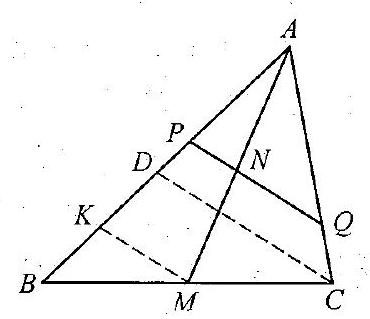
\includegraphics[max width=\textwidth, center]{2024_10_30_2c8f45efd4a519b08e1ag-011}

图1-9

\begin{align*}
\frac{A K}{A P}=\frac{1}{2}\left(\frac{A D}{A P}+\frac{A B}{A P}\right)
\end{align*}

三角形的基本概金和性质。

\section*{厦门郑剑雄高中数学竞赛系列}
全国小学奥数群:221739457,全国初中奥数学生群:253736211,全国高中奥数学生群591782992全国初中奥数教练群112464128,全国高中奥数教练群195949359竞赛公众号:新浪微博@郑剑雄 微信:v136257437 QQ:136257437\\
业务:初高中联赛班、培优班、美国高中数学、教师培训、机构教学产品研发、讲义资料出售等

而

\begin{align*}
\frac{A K}{A P}=\frac{A M}{A N}, \frac{A D}{A P}=\frac{A C}{A Q}
\end{align*}

故

\begin{align*}
\frac{A M}{A N}=\frac{1}{2}\left(\frac{A B}{A P}+\frac{A C}{A Q}\right)=\frac{1}{2}\left(\frac{5}{2}+\frac{4}{3}\right)=\frac{23}{12}
\end{align*}

\section*{习 题 1}
I 有长度为下列数值的几组线段:\\
(i) $3,4,5$ ;(ii) $3^{2}, 4^{2}, 5^{2}$ ;(iii) $\frac{1}{3}, \frac{1}{4}, \frac{1}{5}$ ;(iv) $\frac{1}{3^{2}}, \frac{1}{4^{2}}, \frac{1}{5^{2}}$ 。其中能组成三角形的有()。\\
A. 1 组\\
B. 2 组\\
C. 3 组\\
D. 4 组

2 2 如图, $\angle A+\angle B+\angle C+\angle D+\angle E+\angle F+\angle G$ 的值等于()。\\
A. $360^{\circ}$\\
B. $450^{\circ}$\\
C. $540^{\circ}$\\
D. $720^{\circ}$\\
(2003 年"TRULY 信利杯"联赛题)\\
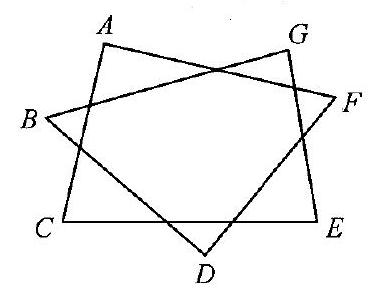
\includegraphics[max width=\textwidth, center]{2024_10_30_2c8f45efd4a519b08e1ag-012(2)}\\
(第2题)\\
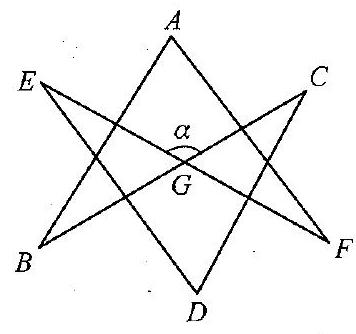
\includegraphics[max width=\textwidth, center]{2024_10_30_2c8f45efd4a519b08e1ag-012}\\
(第3题)

53 如图, $\angle C G E=\alpha$ ,则 $\angle A+\angle B+\angle C+\angle D+\angle E+\angle F=(\quad$.$) 。$\\
A. $360^{\circ}-\alpha$\\
B. $270^{\circ}-\alpha$\\
C. $180^{\circ}+\alpha$\\
D. $2 \alpha$\\
(1999 年山东省竞赛题)\\
4. 如图, $D C$ 平分 $\angle A D B, E C$ 平分 $\angle A E B$, 若 $\angle D A E=\alpha, \angle D B E=\beta$, 则 $\angle D C E=$ $\qquad$ (用 $\alpha, \beta$ 表示)。(1998年山东省竞赛题)\\
5. $\triangle A B C$ 中, $\angle C A B-\angle B=90^{\circ}, \angle C$ 的平分线与 $A B$ 交于 $L, \angle C$ 的外角平分线与 $B A$ 的延长线交于 $N$. 已知 $C L=3$ ,则 $C N=$ $\qquad$。(第1届\\
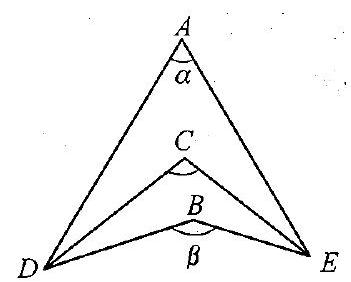
\includegraphics[max width=\textwidth, center]{2024_10_30_2c8f45efd4a519b08e1ag-012(1)}\\
(第4题)\\
"希望杯"邀请赛题)

\section*{夏门郑剑雄高中数学竞赛系列}
全国小学奥数群:221739457,全国初中奥数学生群:253736211,全国高中奥数学生群591782992全国初中奥数教练群112464128,全国高中奥数教练群195949359竞赛公众号:新浪微博@郑剑雄 微信:v136257437 QQ:136257437\\
业务:初高中联赛班、培优班、美国高中数学、教师培训、机构教学产品研发、讲义资料出售等

6 在 $\triangle A B C$ 中, $\angle B=100^{\circ}, \angle C$ 的平分线交边 $A B$ 于 $E$ ,在边 $A C$ 上取点 $D$ ,使得 $\angle C B D=20^{\circ}$ ,连结 $D E$ 。则 $\angle C E D$ 的度数是 $\qquad$。(1993 年北京市竞赛题)\\
7 如图, $C D$ 是 Rt $\triangle A B C$ 斜边 $A B$ 上的高, $\angle A$的平分线 $A E$ 交 $C D$ 于 $H$, 交 $\angle B C D$ 的平分线 $C F$ 于 $G$ 。求证: $H F / / B C$ 。(1995 年天津市竞赛题)\\
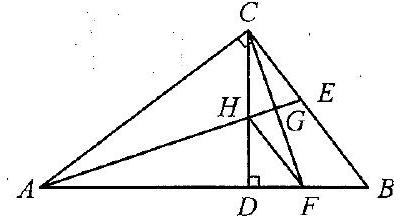
\includegraphics[max width=\textwidth, center]{2024_10_30_2c8f45efd4a519b08e1ag-013}\\
(第7题)

1 三角形的基本概众和性质

\section*{2 \\
 定理}
角形的面积边角间关系\\
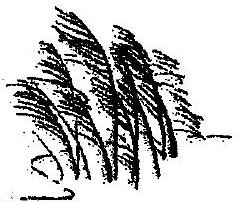
\includegraphics[max width=\textwidth, center]{2024_10_30_2c8f45efd4a519b08e1ag-014(1)}

在 $\triangle A B C$ 中, 设角 $A 、 B 、 C$ 所对的边长依次为 $a 、 b 、 c$, 其面积记为 $S_{\triangle A B C}$, 边长为 $x$ 的边上的高记为 $h_{x}$, 则

\begin{align*}
S_{\triangle A B C}=\frac{1}{2} a h_{a}=\frac{1}{2} b h_{b}=\frac{1}{2} c h_{c} \tag{2-1}
\end{align*}

注意到锐角的三角函数定义,知 $h_{a}=c \cdot \sin B$ 或 $h_{a}=b \cdot \sin C$ ,则

\begin{align*}
S_{\triangle A B C}=\frac{1}{2} a b \cdot \sin C \text { 或 } S_{\triangle A B C}=\frac{1}{2} a c \cdot \sin B \text {. } \tag{2-2}
\end{align*}

若记 $p=\frac{1}{2}(a+b+c)$, 则

\begin{align*}
S_{\triangle A B C}=\sqrt{p(p-a)(p-b)(p-c)} . \text { (海伦公式) } \tag{2-3}
\end{align*}

由上可知:\\
等底等高的两个三角形面积相等;\\
两个等底的三角形的面积比等于底边上对应高的比;\\
两个等高的三角形的面积比等于它们底边的比。\\
作为面积公式及上述结论的一个应用,我们来推导三角形的角平分线性质与外角平分线的性质。

如图 2-1,在 $\triangle A B C$ 中, $A P$ 为 $\angle A$ 的平分线, $A Q$ 为 $\angle A$ 的外角平分线. 由 $\frac{S_{\triangle A B P}}{S_{\triangle A P C}}=\frac{\frac{1}{2} A B \cdot A P \cdot \sin \angle B A P}{\frac{1}{2} A P \cdot A C \cdot \sin \angle P A C}=\frac{A B}{A C}$ 及\\
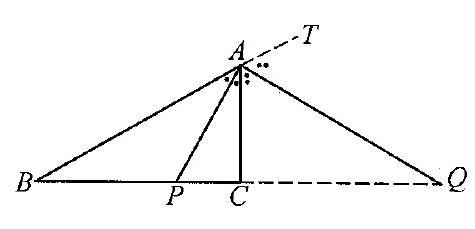
\includegraphics[max width=\textwidth, center]{2024_10_30_2c8f45efd4a519b08e1ag-014}

图 2-1\\
$\frac{S_{\triangle A B P}}{S_{\triangle A P C}}=\frac{B P}{P C}$, 有\\
三角形的角平分线性质定理 $\triangle A B C$ 中, 若 $A P$ 是 $\angle A$ 的平分线, 则

\begin{align*}
\frac{B P}{P C}=\frac{A B}{A C} \tag{2-4}
\end{align*}

又由 $\frac{S_{\triangle A B Q}}{S_{\triangle A C Q}}=\frac{\frac{1}{2} A B \cdot A Q \cdot \sin \angle B A Q}{\frac{1}{2} A C \cdot A Q \cdot \sin \left(180^{\circ}-\angle B A Q\right)}=\frac{A B}{A C}$ 及 $\frac{S_{\triangle A B Q}}{S_{\triangle A B Q}}=\frac{B Q}{Q C}$, 有\\
三角形的外角平分线性质定理 $\triangle A B C$ 中, 若 $A Q$ 是 $\angle A$ 的外角平分线,则

\begin{align*}
\frac{B Q}{Q C}=\frac{A B}{A C} \tag{2-5}
\end{align*}

在同一个三角形中,相等的边所对的角相等,相等的角所对的边相等;较长的边所对的角较大,较大的角所对的边较长。

将面积公式 $S_{\triangle A B C}=\frac{1}{2} a b \sin \angle C=\frac{1}{2} b c \cdot \sin \angle A=\frac{1}{2} c a \cdot \sin \angle B$ 的各项同除以 $\frac{1}{2} a b c$ ,整理(各项倒过来)便得,

正弦定理 在 $\triangle A B C$ 中, 角 $A 、 B 、 C$ 所对的边长分别为 $a 、 b 、 c$, 则

\begin{align*}
\frac{a}{\sin \angle A}=\frac{b}{\sin \angle B}=\frac{c}{\sin \angle C}=\frac{a b c}{2 S_{\triangle A B C}} \tag{2-6}
\end{align*}

对 $\triangle A B C$ 绕顶点 $C$ 顺时针方向旋转 $90^{\circ}$ (这里设 $\angle C \geqslant 90^{\circ}$ ,对于锐角 $\angle C$ 可同样讨论),如图 $2-2$, 得 $\triangle A^{\prime} B^{\prime} C$, 注 意到 $\angle B C B^{\prime}=90^{\circ}$, $\angle A C A^{\prime}=90^{\circ}, \angle A^{\prime}=\angle A, \angle 1=\angle 2$ ,则 $\angle A^{\prime} D A=90^{\circ}$ ( $D$ 为 $A B$ 与 $A^{\prime} B^{\prime}$ 的交点),且 $A^{\prime} B^{\prime}=A B=c$ 。于是

\begin{align*}
\begin{gathered}
S_{\triangle B A^{\prime} B^{\prime}}+S_{\triangle A B^{\prime} A^{\prime}}=S_{\text {四边形 } A^{\prime} A B^{\prime} B} \\
=S_{\triangle B C B^{\prime}}+S_{\triangle A C A^{\prime}}+S_{\triangle B C A^{\prime}}+S_{\triangle A C B^{\prime}},
\end{gathered}
\end{align*}

\begin{center}
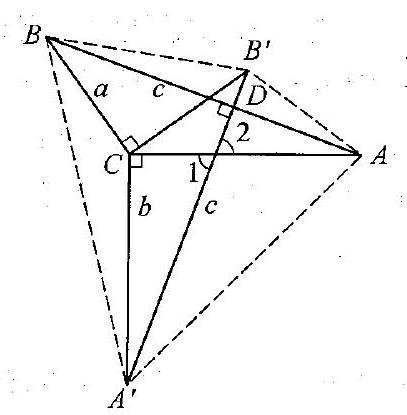
\includegraphics[max width=\textwidth]{2024_10_30_2c8f45efd4a519b08e1ag-015}
\end{center}

图 2-2

即

\begin{align*}
\begin{aligned}
& \frac{1}{2} c \cdot B D+\frac{1}{2} c \cdot A D \\
= & \frac{1}{2} a^{2}+\frac{1}{2} b^{2}+\frac{1}{2} a b \cdot \sin \left[180^{\circ}-\left(\angle C-90^{\circ}\right)\right]+\frac{1}{2} a b \cdot \sin \left(\angle C-90^{\circ}\right),
\end{aligned}
\end{align*}

亦即

\begin{align*}
c^{2}=a^{2}+b^{2}-2 a b \cdot \cos \angle C
\end{align*}

从而便得\\
余弦定理 在 $\triangle A B C$ 中, 角 $A 、 B 、 C$ 所对的边长分别为 $a 、 b 、 c$, 则

2 三角形的面积、奻角间!关系定理

\section*{夏门郑剑雄高中数学竞赛系列}
全国小学奥数群:221739457,全国初中奥数学生群:253736211,全国高中奥数学生群591782992全国初中奥数教练群112464128,全国高中奥数教练群195949359竞赛公众号:新浪微博@郑剑雄 微信:v136257437 QQ:136257437\\
业务:初高中联赛班、培优班、美国高中数学、教师培训、机构教学产品研发、讲义资料出售等

\begin{align*}
\begin{align*}
& c^{2}=a^{2}+b^{2}-2 a b \cdot \cos \angle C, \\
& b^{2}=c^{2}+a^{2}-2 c a \cdot \cos \angle B  \tag{2-7}\\
& a^{2}=b^{2}+c^{2}-2 b c \cdot \cos \angle A .
\end{align*}
\end{align*}

特别地, 当 $\angle C=90^{\circ}$ 时, 则得\\
勾股定理 在 $\triangle A B C$ 中, $\angle C=90^{\circ}$, 则

\begin{align*}
c^{2}=a^{2}+b^{2} \tag{2-8}
\end{align*}

将一个三角形从一个顶点分割为两个三角形,运用面积公式,则得到\\
张角定理 设 $P$ 为 $\triangle A B C$ 的边 $B C$ 上一点, $\angle B A P=\alpha, \angle C A P=$ $\beta$, 则

\begin{align*}
\frac{\sin (\alpha+\beta)}{A P}=\frac{\sin \alpha}{A C}+\frac{\sin \beta}{A B} . \tag{2-9}
\end{align*}

事实上, 如图 2-3, 由 $\frac{1}{2} A B \cdot A C \cdot \sin (\alpha+\beta)=$ $\frac{1}{2} A B \cdot A P \cdot \sin \alpha+\frac{1}{2} A P \cdot A C \cdot \sin \beta$ 两边同除以 $\frac{1}{2} A B \cdot A C \cdot A P$ 即得。

注 张角定理的逆定理为:设 $B 、 P 、 C$ 依次是平面内从一点 $A$ 所引三条射线 $A B 、 A P 、 A C$ 上的\\
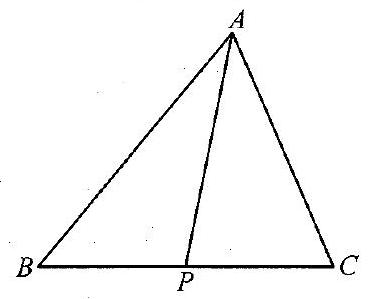
\includegraphics[max width=\textwidth, center]{2024_10_30_2c8f45efd4a519b08e1ag-016}

图2-3

点( $A P$ 在 $A B 、 A C$ 之间), $\angle B A P=\alpha, \angle C A P=$ $\beta$, 且 $\alpha+\beta<180^{\circ}$, 若有

\begin{align*}
\frac{\sin (\alpha+\beta)}{A P}=\frac{\sin \alpha}{A C}+\frac{\sin \beta}{A B},
\end{align*}

则三点 $B 、 P 、 C$ 在一条直线上.\\
事实上,由 $(2-9)$ 式两边同乘以 $\frac{1}{2} A B \cdot A C \cdot A P$ ,整理,即得 $S_{\triangle A B C}=$ $S_{\triangle A B P}+S_{\triangle A C P}$. 这便说明点 $B 、 P 、 C$ 在一条直线上.

对于图2-3中的 $\triangle A B P 、 \triangle A P C$ 应用余弦定理,则得到\\
斯特瓦尔特定理 设 $P$ 为 $\triangle A B C$ 的边 $B C$ 上一点,则

\begin{align*}
A P^{2}=A B^{2} \cdot \frac{P C}{B C}+A C^{2} \cdot \frac{B P}{B C}-B C^{2} \cdot \frac{P C}{B C} \cdot \frac{B P}{B C} \tag{2-10}
\end{align*}

事实上,由 $\frac{A P^{2}+B P^{2}-A B^{2}}{2 A P \cdot B P}=\cos \angle A P B=-\cos \angle A P C=$

\section*{厦门郑剑雄高中数学竞赛系列}
全国小学奥数群:221739457,全国初中奥数学生群:253736211,全国高中奥数学生群591782992全国初中奥数教练群112464128,全国高中奥数教练群195949359竞赛公众号:新浪微博@郑剑雄 微信:v136257437 QQ:136257437\\
业务:初高中联赛班、培优班、美国高中数学、教师培训、机构教学产品研发、讲义资料出售等\\
$-\frac{A P^{2}+P C^{2}-A C^{2}}{2 A P \cdot P C}$ 整理即得。\\
注 若点 $P$ 在边 $B C$ 的延长线上时, 则有 $A P^{2}=-A B^{2} \cdot \frac{P C}{B C}+A C^{2} \cdot$ $\frac{B P}{B C}+B P \cdot P C$; 若点 $P$ 在边 $B C$ 的反向延长线时, 则有 $A P^{2}=A B^{2} \cdot \frac{P C}{B C}-$ $A C^{2} \cdot \frac{B P}{B C}+B P \cdot P C$.

特别地,当 $A P$ 为三角形中的重要线段时,有以下结果。\\
(1) 当 $A P$ 为边 $B C$ 上的中线时,则

\begin{align*}
A P^{2}=\frac{1}{2} A B^{2}+\frac{1}{2} A C^{2}-\frac{1}{4} B C^{2} . \tag{2-11}
\end{align*}

(2)当 $A P$ 为角 $A$ 的平分线时, 则

\begin{align*}
A P^{2}=A B \cdot A C-B P \cdot P C \tag{2-12}
\end{align*}

(3)当 $A P$ 为角 $A$ 的外角平分线时,则

\begin{align*}
A P^{2}=-A B \cdot A C+B P \cdot P C \tag{2-13}
\end{align*}

(4) 当 $\triangle A B C$ 为等腰三角形,即 $A B=A C$ 时,则

\begin{align*}
A P^{2}=A B^{2}-B P \cdot P C \tag{2-14}
\end{align*}

(5)若 $P$ 分线段 $B C$ 满足 $\frac{B P}{B C}=\lambda$ 时,则

\begin{align*}
A P^{2}=\lambda(\lambda-1) B C^{2}+(1-\lambda) \cdot A B^{2}+\lambda \cdot A C^{2} \tag{2-15}
\end{align*}

例1 在 $\triangle A B C$ 中, 已知 $B D$ 和 $C E$ 分别是两边上的中线, 并且 $B D \perp$ $C E, B D=4, C E=6$. 那么, $\triangle A B C$ 的面积等于 $(\quad)$.\\
A. 12\\
B. 14\\
C. 16\\
D. 18\\
(1998 年全国联赛题)\\
解 选 C 。理由:连 $D E$ ,由 $B D \perp C E$ ,知

\begin{align*}
S_{\text {四边形 } B C D E}=\frac{1}{2} B D \cdot C E=12 \text {. }
\end{align*}

注意到 $D 、 E$ 是 $\triangle A B C$ 两边 $A C 、 A B$ 的中点, 知 $S_{\triangle B C D}=S_{\triangle A B D}=2 S_{\triangle A D E}, \quad$ 即 $S_{\text {四边形 } B C D E}=\frac{3}{4} S_{\triangle A B C}$.故 $\quad S_{\triangle A B C}=\frac{4}{3} S_{\text {四边形 } B C D E}=\frac{4}{3} \cdot 12=16$.\\
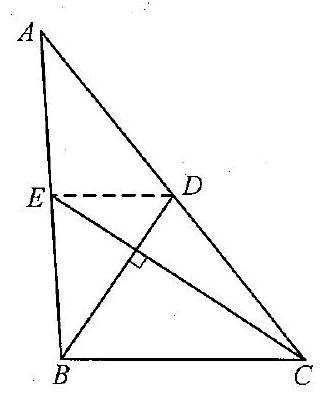
\includegraphics[max width=\textwidth, center]{2024_10_30_2c8f45efd4a519b08e1ag-017}

图2-4\\
2 三角形的面积、边角间关系定理

\section*{夏门郑剑雄高中数学竞赛系列}
全国小学奥数群:221739457,全国初中奥数学生群:253736211,全国高中奥数学生群591782992全国初中奥数教练群112464128,全国高中奥数教练群195949359竞赛公众号:新浪微博@郑剑雄 微信:v136257437 QQ:136257437\\
业务:初高中联赛班、培优班、美国高中数学、教师培训、机构教学产品研发、讲义资料出售等

例2 如图 2-5, 在 $\triangle A B C$ 中, $E F / / B C$, $S_{\triangle A E F}=S_{\triangle B C E}$ 。若 $S_{\triangle A B C}=1$ ,则 $S_{\triangle C E F}$ 等于()。\\
A. $\frac{1}{4}$\\
B. $\frac{1}{5}$\\
C. $\sqrt{5}-2$\\
D. $\sqrt{3}-\frac{3}{2}$\\
(2003 年四川省竞赛题)\\
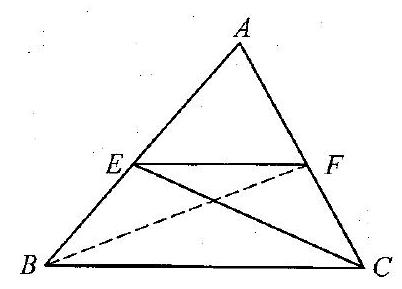
\includegraphics[max width=\textwidth, center]{2024_10_30_2c8f45efd4a519b08e1ag-018(1)}

图2-5

解 选 C. 理由: 设 $S_{\triangle C E F}=x$ ,则

\begin{align*}
\begin{aligned}
& S_{\triangle A E F}=S_{\triangle B C E}=\frac{1}{2}(1-x) \\
& S_{\triangle A E C}=\frac{1}{2}(1+x) \\
& \frac{A F}{A C}=\frac{S_{\triangle A E F}}{S_{\triangle A E C}}=\frac{1-x}{1+x}
\end{aligned}
\end{align*}

于是,

又因为 $E F / / B C$, 所以 $\frac{A E}{A B}=\frac{A F}{A C}$, (或者连 $B F$, 则 $S_{\triangle E F B}=S_{\triangle E F C}$, 所以 $\frac{A E}{A B}=\frac{S_{\triangle A E C}}{S_{\triangle A B C}}=\frac{S_{\triangle A B F}}{S_{\triangle A B C}}=\frac{A F}{A C}$.)从而

\begin{align*}
\frac{S_{\triangle A E F}}{S_{\triangle A B C}}=\frac{\frac{1}{2} A E \cdot A F \cdot \sin A}{\frac{1}{2} A B \cdot A C \cdot \sin A}=\frac{A E \cdot A F}{A B \cdot A C}=\left(\frac{A F}{A C}\right)^{2}=\left(\frac{1-x}{1+x}\right)^{2}
\end{align*}

而

\begin{align*}
\frac{S_{\triangle A E F}}{S_{\triangle A B C}}=\frac{\frac{1}{2}(1-x)}{1}=\frac{1}{2}(1-x),
\end{align*}

故 $\left(\frac{1-x}{1+x}\right)^{2}=\frac{1}{2}(1-x)$. 解得 $x=\sqrt{5}-2$ (舍去 $\left.-2-\sqrt{5}\right)$.\\
例3 如图 2-6, 在 $\triangle A B C$ 中, $D 、 E$ 分别是 $A C 、 B C$ 的中点, $B F=$ $\frac{1}{3} A B, B D$ 与 $F C$ 相交于 $G$, 连结 $E G$ 。\\
(1) 求证: $G E / / A C$;\\
(2)求 $\frac{S_{\triangle B F G}}{S_{\triangle B E G}}$ 的值。 (2001 年重庆市竞赛题)

解 (1)取 $A F$ 的中点 $H$ ,连结 $H D$ ,则知 $H D$ 为 $\triangle A F C$ 的中位线, 即 $D H / / F C$ 。\\
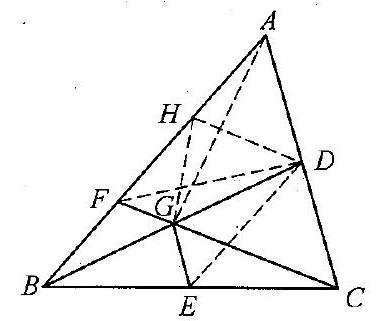
\includegraphics[max width=\textwidth, center]{2024_10_30_2c8f45efd4a519b08e1ag-018}

图 2-6

\section*{厦门郑剑雄高中数学竞赛系列}
全国小学奥数群:221739457,全国初中奥数学生群:253736211,全国高中奥数学生群591782992全国初中奥数教练群112464128,全国高中奥数教练群195949359竞赛公众号:新浪微博@郑剑雄 微信:v136257437 QQ:136257437\\
业务:初高中联赛班、培优班、美国高中数学、教师培训、机构教学产品研发、讲义资料出售等

连 $H G 、 F D$ 。由 $B F=F H, F G / / H D$ ,知 $S_{\triangle B F G}=S_{\triangle H F G}=S_{\triangle D F G}$ ,因此 $B G=G D$, 所以 $G$ 是 $B D$ 的中点. 而 $E$ 是 $B C$ 的中点, 故 $G E / / A C$.\\
(2)连 $A G$, 设 $S_{\triangle B F G}=a$, 则 $S_{\triangle A F G}=2 a$,

\begin{align*}
S_{\triangle A D G}=S_{\triangle A B G}=S_{\triangle B F G}+S_{\triangle A F G}=3 a,
\end{align*}

因此

\begin{align*}
S_{\triangle A B D}=2 S_{\triangle A B G}=6 a, S_{\triangle A B C}=2 S_{\triangle A B D}=12 a,
\end{align*}

亦即

\begin{align*}
S_{\triangle B F G}=\frac{1}{12} S_{\triangle A B C}
\end{align*}

又连 $D E$, 设 $S_{\triangle B E G}=b$, 则

\begin{align*}
\begin{gathered}
S_{\triangle G D E}=b, S_{\triangle B C D}=S_{\triangle B E D}=2 b \\
S_{\triangle B C D}=2 S_{\triangle B E D}=4 b, S_{\triangle A B C}=2 S_{\triangle B C D}=8 b
\end{gathered}
\end{align*}

即

\begin{align*}
\begin{aligned}
& S_{\triangle B E G}=\frac{1}{8} S_{\triangle A B C} \\
& \frac{S_{\triangle B E G}}{S_{\triangle B E G}}=\frac{\frac{1}{12} S_{\triangle A B C}}{\frac{1}{8} S_{\triangle A B C}}=\frac{2}{3}
\end{aligned}
\end{align*}

所以

例 4 如图 2-7, $P$ 是 $\triangle A B C$ 内的一点, 连结 $A P$ 、 $B P 、 C P$ 并延长,分别与 $B C 、 A C 、 A B$ 交于 $D 、 E 、 F$ ,已知: $A P=6, B P=9, P D=6, P E=3, C F=20$ 。求 $\triangle A B C$ 的面积。(第7届美国邀请赛题)

解 由 $A P=6=P D$ ,知 $P$ 为 $A D$ 的中点。过点 $D$ 作 $E A$ 的平行线交 $P B$ 于点 $M$, 则知 $P$ 为 $E M$ 的中点, 即有 $P M=E P=3$, 于是, 点 $M$ 为 $E B$ 的中点. 因此, 知 $D$ 为 $B C$的中点。

过 $D$ 作 $D Q / / A B$ 交 $C P$ 于 $Q$, 则 $C Q=Q F$, $Q P=P F$, 由此, 即知 $P C=15$.\\
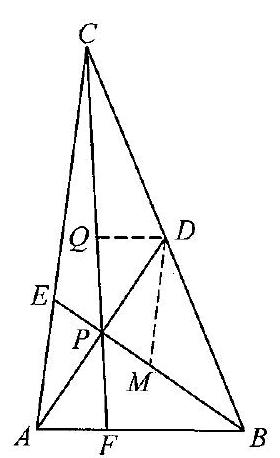
\includegraphics[max width=\textwidth, center]{2024_10_30_2c8f45efd4a519b08e1ag-019}

图2-7

设 $C D=B D=x$ ,则\\
$\triangle C P D$ 的半周长 $=\frac{1}{2}(21+x), \triangle P D B$ 的半周长 $=\frac{1}{2}(15+x)$.\\
由 $S_{\triangle C P D}=S_{\triangle P D B}$ 及海伦公式,得

\begin{align*}
\frac{x+21}{2} \cdot\left(\frac{21+x}{2}-15\right)\left(\frac{21+x}{2}-6\right)\left(\frac{21+x}{2}-x\right)
\end{align*}

2 三角形的面积、边角间关系定理

\section*{夏门郑剑雄高中数学竞赛系列}
全国小学奥数群:221739457,全国初中奥数学生群:253736211,全国高中奥数学生群591782992全国初中奥数教练群112464128,全国高中奥数教练群195949359竞赛公众号:新浪微博@郑剑雄 微信:v136257437 QQ:136257437\\
业务:初高中联赛班、培优班、美国高中数学、教师培训、机构教学产品研发、讲义资料出售等

\begin{align*}
=\frac{x+15}{2} \cdot\left(\frac{15+x}{2}-9\right)\left(\frac{15+x}{2}-6\right)\left(\frac{15+x}{2}-x\right)
\end{align*}

即

\begin{align*}
\begin{aligned}
& (21+x)(x-9)(x+9)(21-x) \\
= & (15+x)(x-3)(x+3)(15-x),
\end{aligned}
\end{align*}

亦即

\begin{align*}
\left(21^{2}-x^{2}\right)\left(x^{2}-9^{2}\right)=\left(15^{2}-x^{2}\right)\left(x^{2}-3^{2}\right)
\end{align*}

由此,解得

\begin{align*}
x^{2}=13 \cdot 9=117
\end{align*}

于是

\begin{align*}
S_{\triangle C P D}^{2}=\frac{1}{16}\left(21^{2}-x^{2}\right)\left(x^{2}-9^{2}\right)=18^{2} \cdot 3^{2} \cdot \frac{1}{4}
\end{align*}

从而

\begin{align*}
S_{\triangle C P D}=27
\end{align*}

又\\
故

\begin{align*}
\begin{gathered}
S_{\triangle P D B}=S_{\triangle P A B}=S_{\triangle P A C}=S_{\triangle C P D}=27, \\
S_{\triangle A B C}=4 S_{\triangle C P D}=108 .
\end{gathered}
\end{align*}

例5 如图 2-8, $O$ 是凸五边形 $A B C D E$ 内一点,且 $\angle 1=\angle 2, \angle 3=$ $\angle 4, \angle 5=\angle 6, \angle 7=\angle 8$ 。求证: $\angle 9$ 与 $\angle 10$ 相等或互补。(1985年全国联赛题)

证明 由题设,根据正弦定理,得

\begin{align*}
\begin{aligned}
\frac{O A}{\sin \angle 10} & =\frac{O E}{\sin \angle 1}=\frac{O E}{\sin \angle 2} \\
& =\frac{O D}{\sin \angle 3}=\frac{O D}{\sin \angle 4} \\
& =\frac{O C}{\sin \angle 5}=\frac{O C}{\sin \angle 6} \\
& =\frac{O B}{\sin \angle 7}=\frac{O B}{\sin \angle 8} \\
& =\frac{O A}{\sin \angle 9}
\end{aligned}
\end{align*}

\begin{center}
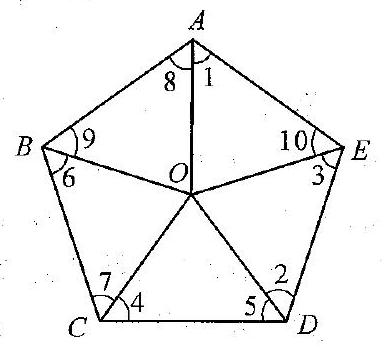
\includegraphics[max width=\textwidth]{2024_10_30_2c8f45efd4a519b08e1ag-020}
\end{center}

图 2-8

从而 $\sin \angle 9=\sin \angle 10$. 故 $\angle 9$ 与 $\angle 10$ 相等或互补。\\
例 6 在 $\triangle A B C$ 中, $A B=33 \mathrm{~cm}, A C=21 \mathrm{~cm}, B C=m \mathrm{~cm}, m$ 为整数,又在 $A B$ 上可找到 $D$, 在 $A C$ 上可找到 $E$ ,使 $A D=D E=E C=n \mathrm{~cm}, n$ 为整数。问 $m$ 可取哪些值。(1983年瑞士奥林匹克题)

解 在 $\triangle A B C$ 中,由余弦定理,有

\begin{align*}
\cos \angle A=\frac{A B^{2}+A C^{2}-B C^{2}}{2 A B \cdot A C}=\frac{33^{2}+21^{2}-m^{2}}{2 \cdot 33 \cdot 21}=\frac{1530-m^{2}}{2 \cdot 7 \cdot 3^{2} \cdot 11}
\end{align*}

又在 $\triangle A D E$ 中, 由余弦定理, 有

全国小学奥数群:221739457,全国初中奥数学生群:253736211,全国高中奥数学生群591782992全国初中奥数教练群112464128,全国高中奥数教练群195949359竞赛公众号:新浪微博@郑剑雄 微信:v136257437 QQ:136257437\\
业务:初高中联赛班、培优班、美国高中数学、教师培训、机构教学产品研发、讲义资料出售等

\begin{align*}
\cos \angle A=\frac{A D^{2}+A E^{2}-D E^{2}}{2 A D \cdot A E}=\frac{n^{2}+(21-n)^{2}-n^{2}}{2 n(21-n)}=\frac{21-n}{2 n} .
\end{align*}

从而有

\begin{align*}
\begin{gathered}
\frac{1530-m^{2}}{2 \cdot 7 \cdot 3^{2} \cdot 11}=\frac{21-n}{2 n}, \\
n\left(2223-m^{2}\right)=3^{3} \cdot 7^{2} \cdot 11
\end{gathered}
\end{align*}

即\\
由于 $m 、 n$ 是正整数,所以, $n$ 是 $3^{3} \cdot 7^{2} \cdot 11$ 的约数。\\
由图2-9知, $E C<A C, A D+D E>A E$ ,则

\begin{align*}
7<n<21
\end{align*}

所以, $n$ 只能取 9 或 11 .\\
当 $n=9$ 时, $m^{2}=2223-3 \cdot 7^{2} \cdot 11=606$ ,由于 606 不是完全平方数, 所以此时无解.

当 $n=11$ 时, $m^{2}=2223-3^{3} \cdot 7^{2}=900$ ,得\\
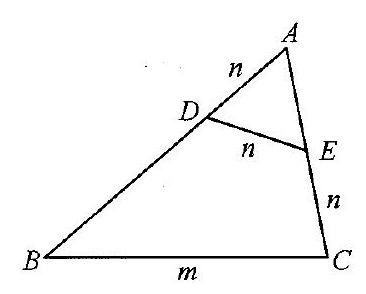
\includegraphics[max width=\textwidth, center]{2024_10_30_2c8f45efd4a519b08e1ag-021(1)}

图2-9\\
$m=30$ 。所以, $m$ 只能取 30 。

例7 已知 $A D 、 A E$ 分别是 $\triangle A B C$ 的角 $A$ 的内、外角平分线, 点 $D$ 在边 $B C$ 上, 点 $E$ 在边 $B C$ 的延长线上。求证: $\frac{1}{B E}+\frac{1}{C E}=\frac{2}{D E}$.

证明 设 $A D=a, A E=b, \angle B A D=$ $\angle D A C=\alpha$.

以 $A$ 为视点,分别在 $\triangle A D E$ 和 $\triangle A B E$ 中应用张角定理,得

于是

\begin{align*}
\begin{aligned}
& \frac{\sin \angle D A E}{A C}=\frac{\sin \alpha}{b}+\frac{\sin \left(90^{\circ}-\alpha\right)}{a} \\
& \frac{\sin \left(90^{\circ}+\alpha\right)}{a}=\frac{\sin \angle D A E}{A B}+\frac{\sin \alpha}{b}
\end{aligned}
\end{align*}

\begin{center}
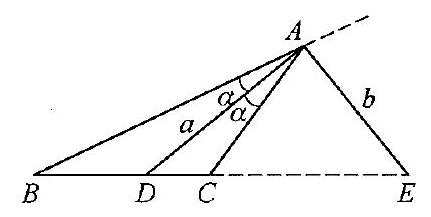
\includegraphics[max width=\textwidth]{2024_10_30_2c8f45efd4a519b08e1ag-021}
\end{center}

图2-10

在 $\triangle A B E$ 中,由余弦定理,并注意到 $\cos \alpha>0$ ,以及 $b \cos \alpha-a \sin \alpha>$ 0 (因 $A B>0$ ),有

\begin{align*}
\begin{aligned}
B E & =\sqrt{A B^{2}+A E^{2}-2 A B \cdot A E \cdot \cos \left(90^{\circ}+\alpha\right)} \\
& =\sqrt{\frac{b^{2} \cdot \cos ^{2} \alpha \cdot\left(a^{2}+b^{2}\right)}{(b \cos \alpha-a \sin \alpha)^{2}}}=\frac{b \cos \alpha \cdot \sqrt{a^{2}+b^{2}}}{b \cos \alpha-a \sin \alpha}
\end{aligned}
\end{align*}

同理,在 $\triangle A C E$ 中,有 $C E=\frac{b \cos \alpha \cdot \sqrt{a^{2}+b^{2}}}{b \cos \alpha+a \sin \alpha}$.\\
2 三角形的面积、边角间\\
关系定理

\section*{夏门郑剑雄高中数学竞赛系列}
全国小学奥数群:221739457,全国初中奥数学生群:253736211,全国高中奥数学生群591782992全国初中奥数教练群112464128,全国高中奥数教练群195949359竞赛公众号:新浪微博@郑剑雄 微信:v136257437 QQ:136257437\\
业务:初高中联赛班、培优班、美国高中数学、教师培训、机构教学产品研发、讲义资料出售等

又在 Rt $\triangle A D E$ 中, 有 $D E=\sqrt{a^{2}+b^{2}}$. 故

\begin{align*}
\frac{1}{B E}+\frac{1}{C E}=\frac{2 b \cos \alpha}{b \cdot \cos \alpha \cdot \sqrt{a^{2}+b^{2}}}=\frac{2}{\sqrt{a^{2}+b^{2}}}=\frac{2}{D E}
\end{align*}

例 8 在 $\triangle A B C$ 中, $A B=2 \sqrt{2}, A C=\sqrt{2}, B C=2$, 设 $P$ 为边 $B C$ 上任一点,则(:)。\\
A. $P A^{2}<P B \cdot P C$\\
B. $P A^{2}=P B \cdot P C$\\
C. $P A^{2}>P B \cdot P C$\\
D. $P A^{2}$ 与 $P B \cdot P C$ 的大小关系不确定\\
(1990 年全国联赛题)

解 选 C. 理由:由斯特瓦尔特定理,有

\begin{align*}
\begin{aligned}
P A^{2} & =A B^{2} \cdot \frac{P C}{B C}+A C^{2} \cdot \frac{P B}{B C}-P B \cdot P C \\
& =(2 \sqrt{2})^{2} \cdot \frac{P C}{2}+(\sqrt{2})^{2} \cdot \frac{P B}{2}-P B \cdot P C \\
& =4 P C+P B-P B \cdot P C
\end{aligned}
\end{align*}

从而

\begin{align*}
P A^{2}-P B \cdot P C=4 P C+P B-2 P B \cdot P C
\end{align*}

又 $P B=2-P C$ ,于是

\begin{align*}
\begin{aligned}
P A^{2}-P B \cdot P C & =4 P C+2-P C-2(2-P C) \cdot P C \\
& =2 P C^{2}-P C+2 \\
& =2\left(P C-\frac{1}{4}\right)^{2}+\frac{15}{8}>0
\end{aligned}
\end{align*}

故

\begin{align*}
P A^{2}>P B \cdot P C
\end{align*}

例 9 在 $\triangle A B C$ 中, $A B=A C=2$, 边 $B C$ 上有 100 个不同的点 $P_{1}$ 、 $P_{2}, \cdots, P_{100}$ 。记 $m_{i}=A P_{i}^{2}+B P_{i} \cdot P_{i} C(i=1,2, \cdots, 100)$ ,则 $m_{1}+m_{2}+\cdots$ $+m_{100}=$ $\qquad$ .(1990年全国联赛题)\\
解 填 400. 理由:由 $A B=A C$ ,考虑斯特瓦尔特定理的特殊情形式 $(2-14)$ ,有 $A P_{i}^{2}=A B^{2}-B P_{i} \cdot P_{i} C(i=1,2, \cdots, 100)$.

于是

\begin{align*}
m_{i}=A P_{i}^{2}+B P_{i} \cdot P_{i} C=A B^{2}=4
\end{align*}

故

\begin{align*}
m_{1}+m_{2}+\cdots+m_{100}=4 \cdot 100=400
\end{align*}

\begin{center}
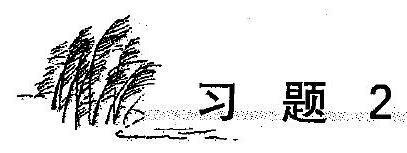
\includegraphics[max width=\textwidth]{2024_10_30_2c8f45efd4a519b08e1ag-022}
\end{center}

1 设 $\triangle A B C$ 的面积是 $1, D$ 是边 $B C$ 上一点, 且 $\frac{B D}{D C}=\frac{1}{2}$. 若在边 $A C$ 上取

\section*{厦门郑剑雄高中数学竞赛系列}
全国小学奥数群:221739457,全国初中奥数学生群:253736211,全国高中奥数学生群591782992全国初中奥数教练群112464128,全国高中奥数教练群195949359竞赛公众号:新浪微博@郑剑雄 微信:v136257437 QQ:136257437\\
业务:初高中联赛班、培优班、美国高中数学、教师培训、机构教学产品研发、讲义资料出售等

一点 $E$, 使四边形 $A B D E$ 的面积为 $\frac{4}{5}$, 则 $\frac{A E}{E C}$ 的值为 $\qquad$ . (2003 年天津市竞赛题)

2 给定面积为 1 , 边长为 $a 、 b 、 c$ 的三角形,已知 $a \geqslant b \geqslant c$ 。求证: $b \geqslant \sqrt{2}$. (第7届全俄奥林匹克题)\\
3 已知三角形的两边长 $a$ 与 $b$ 满足 $a>b$ ,它们对应的高为 $h_{a}$ 与 $h_{b}$ ,求证: $a+h_{a} \geqslant b+h_{b}$ ,并确定等号何时成立。(1967 年英国奥林匹克题)\\
4 直线与 $\triangle A B C$ 的边 $A B$ 和 $B C$ 分别相交于点 $M$ 和 $K$. 又 $\triangle M B K$ 与四边形 $A M K C$ 的面积相等。求证: $\frac{M B+B K}{A M+C A+K C} \geqslant \frac{1}{3}$ 。(第 35 届莫斯科奥林匹克题)\\
5 已知:锐角三角形 $A B C$ 的角平分线 $A D$ ,中线 $B M$ 和高线 $C H$ 交于一点。求证: $\angle B A C>45^{\circ}$ 。(第4届全俄奥林匹克题)\\
6 设 $P 、 Q$ 为线段 $B C$ 上两定点,且 $B P=C Q, A$ 为 $B C$ 外一动点,当点 $A$运动到使 $\angle B A P=\angle C A Q$ 时, $\triangle A B C$ 是什么三角形?试证明你的结论。 (1986 年全国联赛题)\\
7 在 $\triangle A B C$ 中, $\angle A=4 \angle C, \angle B=2 \angle C$. 试证: $(B C+C A) \cdot A B=$ $B C \cdot C A$ 。\\
8. 自 $\triangle A B C$ 的顶点 $A$ 引两条射线交 $B C$ 于 $X 、 Y$, 使 $\angle B A X=\angle C A Y$. 求\\
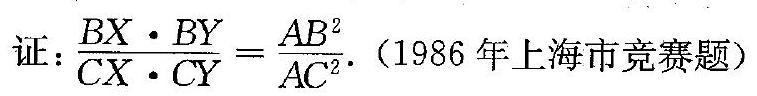
\includegraphics[max width=\textwidth, center]{2024_10_30_2c8f45efd4a519b08e1ag-023}\\
9 设点 $O$ 在 $\triangle A B C$ 的边 $A B$ 上,且与顶点不重合。求证: $O C \cdot A B<O A$ $B C+O B \cdot A C$. (1983 年捷克竞赛题)\\
10 已知 $A B C D$ 为四边形,两组对边延长后得交点 $E 、 F$ ,对角线 $B D / / E F$ , $A C$ 的延长线交 $E F$ 于 $G$ 。求证: $E G=G F$ 。(1978年全国高中竟赛题)\\
I1 在 $\triangle A B C$ 中, $D$ 是 $B C$ 边上的点, 已知 $A B=13, A D=12, A C=15$, $B D=5$ ,那么 $D C$ 等于多少?(第 3 届"祖冲之"杯邀请赛题)

2 三角形的面积边角间关系定理

\section*{厦门郑剑雄高中数学竞赛系列}
全国小学奥数群:221739457,全国初中奥数学生群:253736211,全国高中奥数学生群591782992全国初中奥数教练群112464128,全国高中奥数教练群195949359竞赛公众号:新浪微博@郑剑雄 微信:v136257437 QQ:136257437\\
业务:初高中联赛班、培优班、美国高中数学、教师培训、机构教学产品研发、讲义资料出售等\\
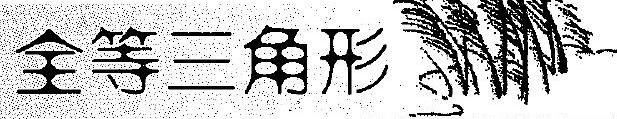
\includegraphics[max width=\textwidth, center]{2024_10_30_2c8f45efd4a519b08e1ag-024}

能够完全重合的两个三角形叫做全等三角形。其中互相重合的顶点叫做对应顶点,互相重合的边叫做对应边,互相重合的角叫做对应角。

实现重合离不开运动,完全重合是运动的结果。至于运动的过程,则有不同的方式。因此,全等三角形的图形归纳起来有以下几种典型形式。\\
(1)平移全等型,如图3-1.\\
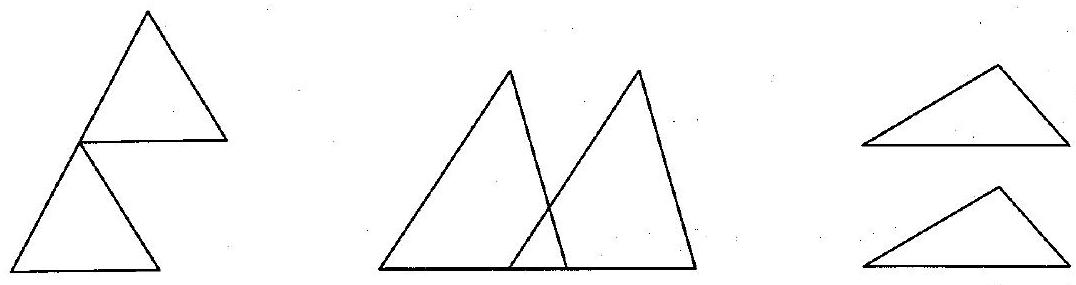
\includegraphics[max width=\textwidth, center]{2024_10_30_2c8f45efd4a519b08e1ag-024(1)}\\
(4)以上类型的复合型,如图 3-4.\\
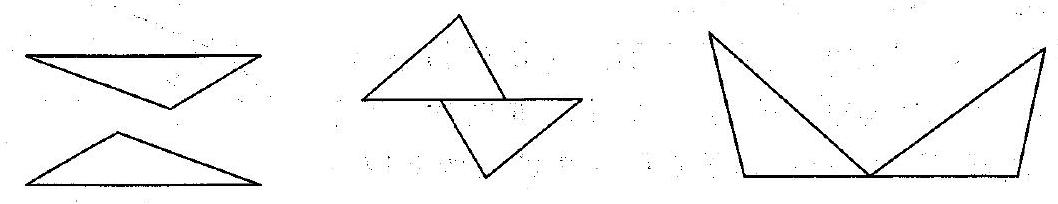
\includegraphics[max width=\textwidth, center]{2024_10_30_2c8f45efd4a519b08e1ag-025}

图3-4\\
全等三角形的对应边相等,对应角相等,三角形中各种对应线段也相等。\\
寻找对应边和对应角,常用到以下方法:\\
(1)全等三角形对应角所对的边是对应边,两个对应角所夹的边是对应边。\\
(2)全等三角形对应边所对的角是对应角,两条对应边所夹的角是对应角。\\
(3)有公共边的,公共边常是对应边。\\
(4)有公共角的,公共角常是对应角。\\
(5)有对顶角的,对顶角常是对应角。\\
(6)两个全等的不等边三角形中一对最长边(或最大角)是对应边(或对应角),一对最短边(或最小角)是对应边(或对应角)。

要想正确表示两个三角形全等,找出对应元素是关键。\\
边角边定理(SAS) 有两条边和它们的夹角对应相等的两个三角形全等。

角边角定理(ASA)有两个角和它们的夹边对应相等的两个三角形全等。

推论 有两个角和其中一个角的对边对应相等的两个三角形全等。\\
边边边定理(SSS) 三边对应相等的两个三角形全等。\\
注 三角形的三边确定了,那么它的形状、大小就确定了。三角形的这个性质,就叫做三角形的稳定性。

由于直角三角形的特殊性,直角三角形全等的判定具有特殊的方法。从理论上讲,不论是"边角边"、角边角"、"边边边",还是"角角边"都适用于直角三角形全等的判定。但直角三角形有如下特殊的判定定理:

斜边、直角边定理(HL)斜边和直角边对应相等的两个直角三角形全等。

由上可知,如果两个直角三角形中有两条边(不论是两条直角边还是斜边和一条直角边)对应相等,就足以判定它们全等。所以,对于直角三角形的全等的判定,"边边边"是没有使用价值的。因此,在两个直角三角形中,如果

\section*{厦门郑剑雄高中数学竞赛系列}
全国小学奥数群:221739457,全国初中奥数学生群:253736211,全国高中奥数学生群591782992全国初中奥数教练群112464128,全国高中奥数教练群195949359竞赛公众号:新浪微博@郑剑雄 微信:v136257437 QQ:136257437\\
业务:初高中联赛班、培优班、美国高中数学、教师培训、机构教学产品研发、讲义资料出售等

除了直角之外,还有两个元素(不都是角)对应相等,那么,这两个直角三角形全等。

例1 设 $P$ 为等腰直角三角形 $A C B$ 的斜边 $A B$上任意一点, $P E$ 垂直 $A C$ 于点 $E, P F$ 垂直 $B C$ 于点 $F, P G$ 垂直 $E F$ 于点 $G$ ,延长 $G P$ 并在延长线上取一点 $D$, 使得 $P D=P C$. 试证: $B C \perp B D$, 且 $B C=$ $B D$ 。(1997 年全国联赛题)\\
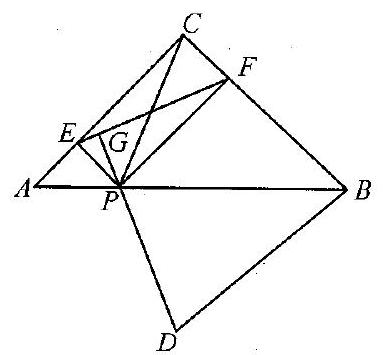
\includegraphics[max width=\textwidth, center]{2024_10_30_2c8f45efd4a519b08e1ag-026(1)}

图3-5

证明 如图 3-5, 因 $\angle E P G=\angle E F P=\angle C P F$ ,

则

\begin{align*}
\begin{aligned}
\angle D P B & =\angle A P G=45^{\circ}+\angle E P G=45^{\circ}+\angle C P F \\
& =\angle B P F+\angle C P F=\angle B P C .
\end{aligned}
\end{align*}

又 $P C=P D, P B$ 为公共边, 则

\begin{align*}
\triangle P D B \cong \triangle P C B .
\end{align*}

从而

\begin{align*}
B C=B D
\end{align*}

且

\begin{align*}
\angle P B D=\angle C B P=45^{\circ},
\end{align*}

因此

\begin{align*}
\angle C B D=90^{\circ},
\end{align*}

故\\
$B C \perp B D$.\\
例2 已知: $B D 、 C E$ 是 $\triangle A B C$ 的高, 点 $P$ 在 $B D$ 的延长线上, $B P=$ $A C$ ,点 $Q$ 在 $C E$ 上, $C Q=A B$ ,求证:(1) $A P=A Q$ ;(2) $A P \perp A Q$ 。(1996年河南省竞赛题)

证明 如图 3-6,设 $C E$ 交 $B D$ 于 $F$ 。\\
(1) 由 $B D \perp C A, C E \perp A B$ ,知

\begin{align*}
\angle B E F=90^{\circ}=\angle C D F .
\end{align*}

而

\begin{align*}
\angle B F E=\angle C F D
\end{align*}

故

\begin{align*}
\angle A B P=\angle Q C A
\end{align*}

\begin{center}
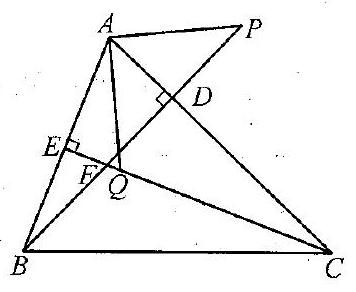
\includegraphics[max width=\textwidth]{2024_10_30_2c8f45efd4a519b08e1ag-026}
\end{center}

图3-6

由已知, 有 $A B=Q C, B P=C A$, 从而

\begin{align*}
\triangle A B P \cong \triangle Q C A,
\end{align*}

即有

\begin{align*}
A P=A Q
\end{align*}

(2)由(1)可得 $\angle A Q C=\angle P A B$ ,而

\begin{align*}
\angle A Q C=\angle Q E A+\angle Q A E=90^{\circ}+\angle Q A E,
\end{align*}

厦门郑剑雄高中数学竞赛系列\\
全国小学奥数群:221739457,全国初中奥数学生群:253736211,全国高中奥数学生群591782992全国初中奥数教练群112464128,全国高中奥数教练群195949359竞赛公众号:新浪微博@郑剑雄 微信:v136257437 QQ:136257437\\
业务:初高中联赛班、培优班、美国高中数学、教师培训、机构教学产品研发、讲义资料出售等

\begin{align*}
\angle P A B=\angle P A Q+\angle Q A E,
\end{align*}

从而可得

\begin{align*}
\angle P A Q=90^{\circ},
\end{align*}

即

\begin{align*}
A P \perp A Q
\end{align*}

例3 在正 $\triangle A B C$ 内部有一点 $O$, 已知 $\angle A O B=113^{\circ}, \angle B O C=123^{\circ}$ 。若一个三角形的边长等于 $O A 、 O B 、 O C$. 试求 : 这个三角形的各角度数。(第 33届莫斯科奥林匹克题)

解 如图 3-7, 以 $A O$ 为一边作等边 $\triangle A D O$ ,连 $B D$. 由

\begin{align*}
A D=A O, A B=A C
\end{align*}

\begin{align*}
\angle D A B=60^{\circ}-\angle B A O=\angle O A C
\end{align*}

则有

\begin{align*}
\triangle A D B \cong \triangle A O C
\end{align*}

所以 $D B=O C, \angle A D B=\angle A O C=124^{\circ}$.\\
又 $O D=O A$, 则 $\triangle O D B$ 的三边的长分别等于 $O A 、 O B 、 O C$ ,而\\
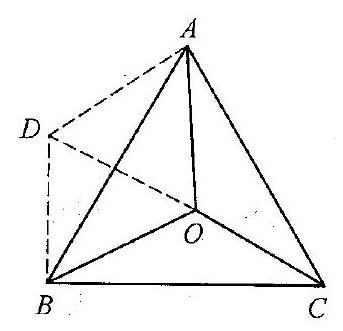
\includegraphics[max width=\textwidth, center]{2024_10_30_2c8f45efd4a519b08e1ag-027}

图3-7

\begin{align*}
\begin{gathered}
\angle D O B=\angle A O B-\angle A O D=113^{\circ}-60^{\circ}=53^{\circ}, \\
\angle O D B=\angle A D B-\angle A D O=124^{\circ}-60^{\circ}=64^{\circ}, \\
\angle O B D=180^{\circ}-53^{\circ}-64^{\circ}=63^{\circ} .
\end{gathered}
\end{align*}

故所求三角形内角分别为 $53^{\circ} 、 64^{\circ} 、 63^{\circ}$.\\
例4 如图 3-8, 在 $\triangle A B C$ 中, $A B=A C, D$ 是底边 $B C$ 上一点, $E$ 是线段 $A D$ 上一点, 且 $\angle B E D=2 \angle C E D=\angle B A C$, 求证: $B D=2 C D$ 。(1992年全国联赛题)

证明 作 $\angle B E D$ 的平分线交 $B C$ 于 $F$ ,又过 $A$作 $A H / / E F$ 交 $B E$ 于 $G$ ,交 $B C$ 于 $H$ ,则知

\begin{align*}
\begin{aligned}
\angle E A G & =\angle D E F=\angle B E F \\
& =\angle A G E=\frac{1}{2} \angle B A C
\end{aligned}
\end{align*}

从而

\begin{align*}
G E=A E
\end{align*}

\begin{align*}
\text { 又 } \angle A G E=\frac{1}{2} \angle B E D=\angle C E D \text {, 则 }
\end{align*}

\begin{center}
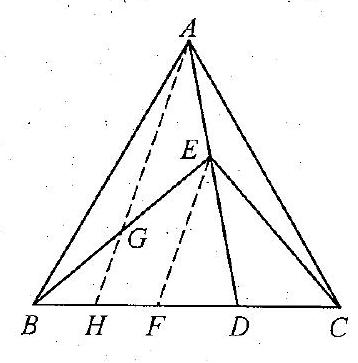
\includegraphics[max width=\textwidth]{2024_10_30_2c8f45efd4a519b08e1ag-027(1)}
\end{center}

图 3-8

\begin{align*}
\angle A G B=\angle C E A
\end{align*}

由

\begin{align*}
\begin{gathered}
\angle A B E+\angle B A E=\angle B E D=\angle B A C=\angle C A E+\angle B A E, \\
\angle A B G=\angle C A E .
\end{gathered}
\end{align*}

有

注意到 $A B=C A$ ,故有

\begin{align*}
\triangle A B G \cong \triangle C A E
\end{align*}

从而,

\begin{align*}
B G=A E, A G=C E
\end{align*}

于是

\begin{align*}
B G=G E
\end{align*}

又由 $A H / / E F$ ,有

且

\begin{align*}
\begin{gathered}
B H=H F, G H=\frac{1}{2} E F . \\
\frac{A H}{E F}=\frac{H D}{F D}
\end{gathered}
\end{align*}

而 $\angle C E D=\angle F E D$ ,从而

\begin{align*}
\frac{C D}{F D}=\frac{E \dot{C}}{E F}=\frac{A G}{E F}=\frac{A H-G H}{E F}=\frac{A H}{E F}-\frac{1}{2}=\frac{H D}{F D}-\frac{1}{2},
\end{align*}

即

\begin{align*}
C D=H D-\frac{1}{2} F D=H F+\frac{1}{2} F D=\frac{1}{2} B F+\frac{1}{2} F D=\frac{1}{2} B D,
\end{align*}

故

\begin{align*}
B D=2 C D
\end{align*}

例5 在 $\triangle A B C$ 中, $\angle B A C=80^{\circ}, \angle A B C=60^{\circ}, D$ 为三角形内一点,且 $\angle D A B=10^{\circ}, \angle D B A=20^{\circ}$. 求 $\angle A C D$ 的度数。

解 如图 3-9, 延长 $B D$ 交 $A C$ 于 $E$, 则 $\angle A E B=80^{\circ}=\angle B A E, A B=B E$ 。在 $B C$ 上截取 $B F=B A$ ,连 $A F$ ,则 $\triangle A B F$ 为等边三角形。在 $A C$上截取 $A G=A B$ ,连 $B G 、 D G 、 E F 、 F G$ 。

由边角边定理:知等腰 $\triangle A F G \cong$ 等腰 $\triangle B A E$ 。\\
在 $\triangle B E F$ 中,因 $B E=B F, \angle E B F=40^{\circ}$ ,则 $\angle B E F=70^{\circ}$, 易得 $\angle F E G=30^{\circ}=\angle A D E$ 。\\
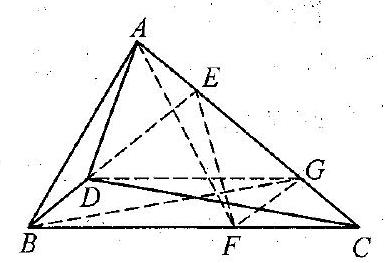
\includegraphics[max width=\textwidth, center]{2024_10_30_2c8f45efd4a519b08e1ag-028}

图3-9

由角边角定理,知 $\triangle F E G \cong \triangle A D E$ 。于是 $E G=D E$ 。\\
注意到 $\angle E B C=40^{\circ}=\angle E C B$ ,故 $E C=E B$ 。\\
又由边角边定理,知 $\triangle E D C \cong \triangle E G B$ ,从而 $\angle A C D=\angle E B G$ 。\\
在 $\triangle A B G$ 中, 因 $A B=A G, \angle B A G=80^{\circ}$, 则 $\angle A B G=50^{\circ}$, 从而 $\angle E B G=30^{\circ}$ 。故 $\angle A C D=30^{\circ}$ 。

例6 在 $\triangle A B C$ 中, $\angle B A C=5.25^{\circ}, A D$ 是 $\angle B A C$ 的平分线, 过 $A$ 作 $D A$ 的垂线交直线 $B C$ 于点 $M$. 若 $B M=B A+A C$, 试求 $\angle A B C$ 和 $\angle A C B$ 的度数。(1991年北京市竞赛题)

\section*{厦门郑剑雄高中数学竞赛系列}
全国小学奥数群:221739457,全国初中奥数学生群:253736211,全国高中奥数学生群591782992全国初中奥数教练群112464128,全国高中奥数教练群195949359竞赛公众号:新浪微博@郑剑雄 微信:v136257437 QQ:136257437\\
业务:初高中联赛班、培优班、美国高中数学、教师培训、机构教学产品研发、讲义资料出售等

解 由于点 $M$ 在直线 $B C$ 上,因而应分两种情况讨论计算:\\
(1)如图3-10,过 $A$ 作 $A D$ 的垂线交 $B C$ 延长线于点 $M$, 延长 $B A$ 到 $C_{1}$, 使 $\angle A M C_{1}=\angle A M C$ 。

由题设 $A D$ 平分 $\angle B A C$ 知 $\angle C A M=\angle C_{1} A M$,注意到 $A M$ 为公共边,则由角边角定理得 $\triangle A C M \cong$ $\triangle A C_{1} M$. 于是, 有 $A C_{1}=A C$. 又由 $B M=B A+A C$,\\
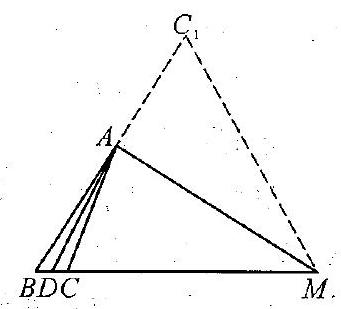
\includegraphics[max width=\textwidth, center]{2024_10_30_2c8f45efd4a519b08e1ag-029(1)}

图3-10

知 $B C_{1}=B M$ 。从而

\begin{align*}
\angle A C_{1} M=\angle B M C_{1}
\end{align*}

在 $\triangle B C_{1} M$ 中,

\begin{align*}
\begin{aligned}
\angle B & =180^{\circ}-2 \angle A C_{1} M=180^{\circ}-2 \angle A C M \\
& =180^{\circ}-2\left(\angle B+5.25^{\circ}\right) \\
& =180^{\circ}-2 \angle B-10.5^{\circ}
\end{aligned}
\end{align*}

因此,

\begin{align*}
\angle A B C=56.5^{\circ},
\end{align*}

\begin{align*}
\angle A C B=180^{\circ}-5.25^{\circ}-56.5^{\circ}=118.25^{\circ}
\end{align*}

(2)如图 3-11,过 $A$ 作 $A D$ 的垂线交 $C B$ 延长线于点 $M$ ,延长 $B A$ 到 $C_{1}$ ,使 $\angle A M C_{1}=\angle A M C$ 。

由题设 $A D$ 平分 $\angle B A C$ 知 $\angle C A M=\angle C_{1} A M$ ,注意到 $A M$ 为公共边,则 $\triangle A C M \cong \triangle A C_{1} M$ ,即有 $\angle A C M=\angle A C_{1} M$ 且 $A C_{1}=A C$.

又由 $B M=B A+A C$, 知 $B C_{1}=B M$. 从而

\begin{align*}
\angle A C_{1} M=\angle B M C_{1}
\end{align*}

\begin{center}
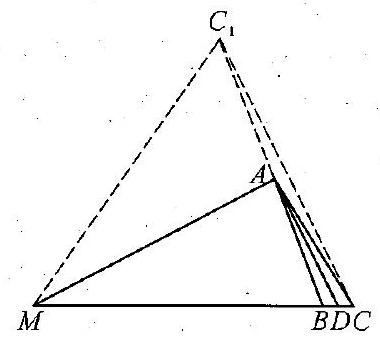
\includegraphics[max width=\textwidth]{2024_10_30_2c8f45efd4a519b08e1ag-029}
\end{center}

图3-11

于是, 在 $\triangle M C C_{1}$ 中,

\begin{align*}
3 \angle A C M+2 \angle A C C_{1}=3 \angle A C M+\angle B A C=180^{\circ},
\end{align*}

即有

\begin{align*}
\angle A C M=\frac{1}{3}\left(180^{\circ}-\angle B A C\right)=58.25^{\circ}
\end{align*}

即

\begin{align*}
\begin{gathered}
\angle A C B=58.25^{\circ} \\
\angle A B C=180^{\circ}-58.25^{\circ}-5.25^{\circ}=116.5^{\circ}
\end{gathered}
\end{align*}

例7 求证:如果两个三角形有两条边和第三条边上的中线对应相等,那么这两个三角形全等。

已知:如图 $3-12$, 在 $\triangle A B C$ 和 $\triangle A^{\prime} B^{\prime} C^{\prime}$ 中, $A D 、 A^{\prime} D^{\prime}$ 分别是边 $B C$ 、\\
$B^{\prime} C^{\prime}$ 上的中线, $A B=A^{\prime} B^{\prime}, A C=$ $A^{\prime} C^{\prime}, A D=A^{\prime} D^{\prime}$ 。

求证: $\triangle A B C \cong \triangle A^{\prime} B^{\prime} C^{\prime}$ 。\\
证明 分别延长 $A D 、 A^{\prime} D^{\prime}$ 至 $E 、 E^{\prime}$ ,使 $D E=A D, D^{\prime} E^{\prime}=A^{\prime} D^{\prime}$ 。连结 $B E$ 、 $B^{\prime} E^{\prime}$ ,则 $A E=2 A D, A^{\prime} E^{\prime}=2 A^{\prime} D^{\prime}$ 。

因为 $A D=A^{\prime} D^{\prime}$ ,所以 $A E=A^{\prime} E^{\prime}$ 。\\
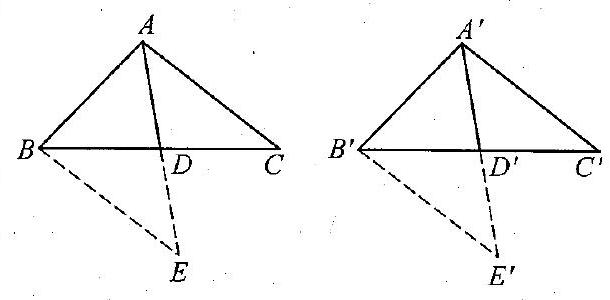
\includegraphics[max width=\textwidth, center]{2024_10_30_2c8f45efd4a519b08e1ag-030}

图3-12

在 $\triangle A D C$ 和 $\triangle E D B$ 中, 由 $A D=$ $D E, \angle A D C=\angle E D B, B D=D C$, 知 $\triangle A D C \cong \triangle E D B$, 从而 $A C=B E$, $\angle E=\angle C A D$.

同理, $\triangle A^{\prime} D^{\prime} C^{\prime} \cong \triangle E^{\prime} D^{\prime} B^{\prime}$ ,有 $A^{\prime} C^{\prime}=B^{\prime} E^{\prime}, \angle E^{\prime}=\angle C^{\prime} A^{\prime} D^{\prime}$ 。\\
因为 $A C=A^{\prime} C^{\prime}$ ,所以 $B E=B^{\prime} E^{\prime}$ 。\\
在 $\triangle A B E$ 和 $\triangle A^{\prime} B^{\prime} E^{\prime}$ 中, 由 $A B=A^{\prime} B^{\prime}, B E=B^{\prime} E^{\prime}, A E=A^{\prime} E^{\prime}$ ,所以,有 $\triangle A B E \cong \triangle A^{\prime} B^{\prime} E^{\prime}$ 。从而 $\angle E=\angle E^{\prime}, \angle B A E=\angle B^{\prime} A^{\prime} E^{\prime}$ ,所以 $\angle C A D=\angle E=\angle E^{\prime}=\angle C^{\prime} A^{\prime} D^{\prime}$, 所以 $\angle B A C=\angle B^{\prime} A^{\prime} C^{\prime}$ 。

在 $\triangle A B C$ 和 $\triangle A^{\prime} B^{\prime} C^{\prime}$ 中, 由 $A B=A^{\prime} B^{\prime}, \angle B A C=\angle B^{\prime} A^{\prime} C^{\prime}, A C=$ $A^{\prime} C^{\prime}$ ,故 $\triangle A B C \cong \triangle A^{\prime} B^{\prime} C^{\prime}$ 。

例8 在 $\triangle A B C$ 中, $D$ 为 $A B$ 的中点, 分别延长 $C A 、 C B$ 到点 $E 、 F$, 使 $D E=D F$ 。过 $E 、 F$ 分别作直线 $C A 、 C B$ 的垂线,相交于点 $P$, 设线段 $P A 、 P B$ 的中点分别为 $M$ 、 $N$. 求证:\\
(1) $\triangle D E M \cong \triangle F D N$;\\
(2) $\angle P A E=\angle P B F$.\\
(2003 年全国联赛题)\\
证明 (1)如图3-13,根据题设可知,

\begin{align*}
D M \cong B N, D N \cong A M .
\end{align*}

所以

\begin{align*}
\angle A M D=\angle A P B=\angle B N D .
\end{align*}

\begin{center}
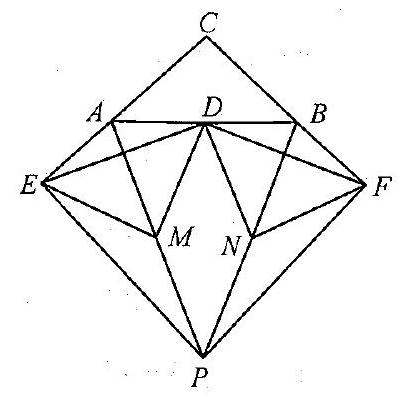
\includegraphics[max width=\textwidth]{2024_10_30_2c8f45efd4a519b08e1ag-030(1)}
\end{center}

图3-13

因为 $M 、 N$ 分别是直角三角形 $\triangle A E P 、 \triangle B F P$ 的斜边的中点,所以

\begin{align*}
\begin{aligned}
& E M=A M=D N \\
& F N=B N=D M
\end{aligned}
\end{align*}

又已知 $D E=D F$ ,从而

\begin{align*}
\triangle D E M \cong \triangle F D N
\end{align*}

(2)由(1)可知 $\angle E M D=\angle F N D$ ,则由 $\angle A M D=\angle D N B$ 可得

\section*{夏门郑剑雄高中数学竞赛系列}
全国小学奥数群:221739457,全国初中奥数学生群:253736211,全国高中奥数学生群591782992全国初中奥数教练群112464128,全国高中奥数教练群195949359竞赛公众号:新浪微博@郑剑雄 微信:v136257437 QQ:136257437\\
业务:初高中联赛班、培优班、美国高中数学、教师培训、机构教学产品研发、讲义资料出售等

\begin{align*}
\angle A M E=\angle B N F .
\end{align*}

而 $\triangle A M E 、 \triangle B N F$ 均为等腰三角形,所以

\begin{align*}
\angle P A E=\angle P B F .
\end{align*}

例9 试证明:有两条边及一个角的角平分线对应相等的两个三角形全等。

证明 设 $\triangle A B C$ 和 $\triangle A^{\prime} B^{\prime} C^{\prime}$ 的三边之长分别记为 $a 、 b 、 c$ 和 $a^{\prime} 、 b^{\prime} 、 c^{\prime}$,三条角平分线长分别记为 $t_{a} 、 t_{b} 、 t_{c}$ 和 $t^{\prime}{ }_{a} 、 t^{\prime}{ }_{b} 、 t^{\prime}{ }_{c}$ ,半周长分别记为 $p$ 和 $p^{\prime}$ 。

当有两条边及它们的夹角的平分线对应相等时,不妨设 $b=b^{\prime}, c=c^{\prime}$ , $t_{a}=t^{\prime}{ }_{a}$.

利用角的平分线性质计算得

\begin{align*}
B P \cdot P C=\frac{a^{2} b c}{(b+c)^{2}},
\end{align*}

注意到斯特瓦尔特定理的特殊情形,即式(2-12),可得到

\begin{align*}
\begin{aligned}
t_{a} & =\frac{2}{b+c} \sqrt{b c p(p-a)} \\
t_{a}^{\prime} & =\frac{2}{b^{\prime}+c} \sqrt{b^{\prime} c^{\prime} p^{\prime}\left(p^{\prime}-a^{\prime}\right)}
\end{aligned}
\end{align*}

由 $b=b^{\prime}, c=c^{\prime}, t_{a}=t_{a}^{\prime}$, 有

\begin{align*}
\frac{2}{b+c} \sqrt{b c p \cdot(p-a)}=\frac{2}{b+c} \sqrt{b c p^{\prime}\left(p^{\prime}-a^{\prime}\right)},
\end{align*}

即有

\begin{align*}
p(p-a)=p^{\prime}\left(p^{\prime}-a^{\prime}\right),
\end{align*}

亦即有

\begin{align*}
(b+c+a)(b+c-a)=\left(b+c+a^{\prime}\right)\left(b+c-a^{\prime}\right)
\end{align*}

从而得

\begin{align*}
a=a^{\prime},
\end{align*}

所以

\begin{align*}
\triangle A B C \cong \triangle A^{\prime} B^{\prime} C^{\prime} .
\end{align*}

当有两条边及其中一边的对角的平分线对应相等时,不妨设

\begin{align*}
a=a^{\prime}, b=b^{\prime}, t_{a}=t_{a}^{\prime}
\end{align*}

此时,有

\begin{align*}
\begin{aligned}
& \frac{2}{b+c} \sqrt{b c \cdot \frac{b+c+a}{2} \cdot \frac{b+c-a}{2}} \\
= & \frac{2}{b+c} \sqrt{b c^{\prime} \cdot \frac{b+c^{\prime}+a}{2} \cdot \frac{b+c^{\prime}-a}{2}}
\end{aligned}
\end{align*}

两边平方,得

即有

\begin{align*}
\frac{c(b+c)^{2}-c a^{2}}{(b+c)^{2}}=\frac{c^{\prime}\left(b+c^{\prime}\right)^{2}-c^{\prime} a^{2}}{\left(b+c^{\prime}\right)^{2}}
\end{align*}

\begin{align*}
\left(c-c^{\prime}\right)+a^{2}\left[\frac{c^{\prime}}{\left(b+c^{\prime}\right)^{2}}-\frac{c}{(b+c)^{2}}\right]=0 .
\end{align*}

即有

\begin{align*}
\left(c-c^{\prime}\right)+\frac{a^{2}\left(c^{\prime}-c\right)\left(b^{2}-c c^{\prime}\right)}{(b+c)^{2}\left(b+c^{\prime}\right)^{2}}=0
\end{align*}

所以

\begin{align*}
\left(c-c^{\prime}\right)\left[(b+c)^{2}\left(b+c^{\prime}\right)^{2}-a^{2} b^{2}+a^{2} c c^{\prime}\right]=0 .
\end{align*}

而

\begin{align*}
(b+c)^{2}\left(b+c^{\prime}\right)^{2}>(b+c)^{2} b^{2}>a^{2} b^{2},
\end{align*}

故由(*)式知

\begin{align*}
c-c^{\prime}=0, \quad \text { 即 } c=c^{\prime} \text {. }
\end{align*}

\section*{从而}
\begin{align*}
\triangle A B C \cong \triangle A^{\prime} B^{\prime} C^{\prime}
\end{align*}

注 由此例及例 7 可知,如果两个三角形有两条边对应相等,再加上一条中线或一条角平分线对应相等,则两个三角形必全等。而加上任一条高线对应相等则不一定全等。

例10 试证直角三角形的如下性质:\\
(1)直角三角形斜边上的中线长等于斜边的一半;\\
(2)直角三角形的斜边等于一条直角边的两倍,则此直角边所对的角为 $30^{\circ}$ 。\\
证明 如图 3-14 设在 Rt $\triangle A B C$ 中, $\angle C=90^{\circ}$ 。\\
(1)在边 $A C$ 上取中点 $D$ ,过 $D$ 作垂线交 $A B$ 于 $M$, 则 $D M / / C B$, 且 $M$ 为 $A B$ 的中点, 即 $B M=M A$ 。连 $C M$ ,在 Rt $\triangle C D M$ 和 Rt $\triangle A D M$ 中,

\begin{align*}
C D=D A, \quad D M \text { 为公共边, }
\end{align*}

故

\begin{align*}
\text { Rt } \triangle C D M \cong \text { Rt } \triangle A D M
\end{align*}

\begin{center}
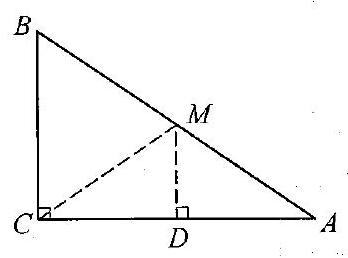
\includegraphics[max width=\textwidth]{2024_10_30_2c8f45efd4a519b08e1ag-032}
\end{center}

图3-14

从而 $C M=A M$. 故 $C M=\frac{1}{2} A B$ 。\\
(2) 设斜边 $A B=2 B C$, 在 $A B$ 边上取中点 $M$, 连 $C M$, 则由 (1) 中结论, 知 $C M=\frac{1}{2} A B=B M$. 于是 $\triangle B C M$ 为等边三角形, 即 $\angle B=60^{\circ}$.

故 $\angle A=30^{\circ}$ 。\\
注 这是两个非常有用的结论。对于(1)的逆命题显然是成立的;对于 (2)的逆命题:若三角形的一边长等于最短边的两倍,且最短边所对的角为 $30^{\circ}$ 时,则此三角形为直角三角形。类似(1)的证明,运用直角三角形全等可证

\section*{夏门郑剑雄高中数学竞赛系列}
全国小学奥数群:221739457,全国初中奥数学生群:253736211,全国高中奥数学生群591782992全国初中奥数教练群112464128,全国高中奥数教练群195949359竞赛公众号:新浪微博@郑剑雄 微信:v136257437 QQ: 136257437\\
业务:初高中联赛班、培优班、美国高中数学、教师培训、机构教学产品研发、讲义资料出售等

明此结论也是成立的。\\
例11 如图 3-15,等腰直角三角形 $\triangle A B C$中, $\angle B A C=90^{\circ}, A D=A E, A F \perp B E$ 交 $B C$于点 $F$ ,过 $F$ 作 $F G \perp C D$ 交 $B E$ 延长线于点 $G$ 。求证: $B G=A F+F G$ 。(1999 年重庆市竟赛题)

证明 过 $C$ 作 $A B$ 的平行线交 $A F$ 的延长线于 $P$ ,则 $P C \perp A C$ 。在 $\mathrm{Rt} \triangle A B E$ 和 $\mathrm{Rt} \triangle C A P$中,由 $A P \perp B E$ ,有 $\angle A B E=\angle C A P$ ,又 $A B=$\\
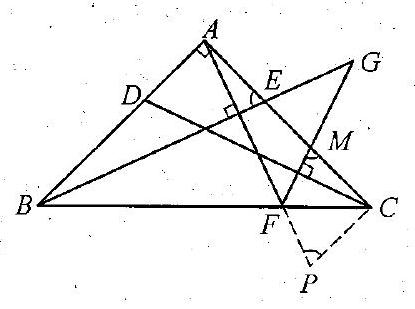
\includegraphics[max width=\textwidth, center]{2024_10_30_2c8f45efd4a519b08e1ag-033}

图3-15\\
$A C$ ,故 Rt $\triangle A B E \cong$ Rt $\triangle C A P$ 。于是

\begin{align*}
\begin{gather*}
\angle A E B=\angle C P A \\
B E=A P .
\end{gather*} \tag{1}
\end{align*}

在 Rt $\triangle A B E$ 和 Rt $\triangle A C D$ 中, $A B=A C, A E=A D$ ,则 Rt $\triangle A B E \cong$ $\mathrm{Rt} \triangle A C D$ 。从而

\begin{align*}
\angle A B E=\angle A C D
\end{align*}

因为 $\angle A E B$ 和 $\angle C M F(A C$ 交 $F G$ 于 $M$ ) 分别是 $\angle A B E$ 和 $\angle A C D$ 的余角,所以

\begin{align*}
\angle A E B=\angle C M F \text {, 则 } \angle F M C=\angle C P A \text {. }
\end{align*}

由 $\angle A C B=45^{\circ}$, 则 $\angle F C P=90^{\circ}-45^{\circ}=45^{\circ}$, 从而

\begin{align*}
\angle M C F=\angle F C P .
\end{align*}

又 $F C$ 公用, 故 $\triangle M C F \cong \triangle P C F$. 于是

\begin{align*}
M F=P F \tag{2}
\end{align*}

又由 $\angle A E B=\angle C M F$, 知 $\triangle M G E$ 为等腰三角形, 则

\begin{align*}
E G=M G \tag{3}
\end{align*}

由(1)、(2)、(3)知,

\begin{align*}
B E+E G=A P+M G=A F+F P+M G=A F+F M+M G
\end{align*}

即

\begin{align*}
B G=A F+F G
\end{align*}

例12 如图 3-16, 已知 Rt $\triangle A B C$ 中, $C D$ 是斜边 $A B$ 上的高, $O 、 O_{1} 、 O_{2}$分别是 $\triangle A B C 、 \triangle A C D 、 \triangle B C D$ 的角平分线的交点. 求证:(1) $O_{1} O \perp C O_{2}$ ; (2) $O C=O_{1} O_{2}$. (1999 年武汉市竞赛题)

证明(1)由题设 $O_{1} 、 O$ 都在 $\angle A$ 的平分线上, 设该平分线交 $\mathrm{CO}_{2}$ 于 $E$. 由 $\angle A=\angle D C B$, 有 $\angle E A C=\angle O_{2} C B, \angle E A C+\angle A C E=\angle O_{2} C B+$ $\angle A C E=90^{\circ}$, 即 $\angle A E C=90^{\circ}$ ,故 $O_{1} O \perp C O_{2}$ 。\\
(2) 由于点 $O_{1} 、 O_{2}$ 分别在 $\angle A C D$ 和 $\angle D C B$ 的平分线上, 则 $\angle O_{1} C O_{2}=45^{\circ}$ 。由 (1) 知 $\angle O_{1} E C=$ $90^{\circ}$ ,所以有 $C E=E O_{1}$ 。

同理,设直线 $O_{2} O$ 交 $C O_{1}$ 于 $F$ ,则 $O_{2} F \perp C F$ , $\angle O O_{2} E=45^{\circ}$ ,有 $E O=O_{2} E$ 。\\
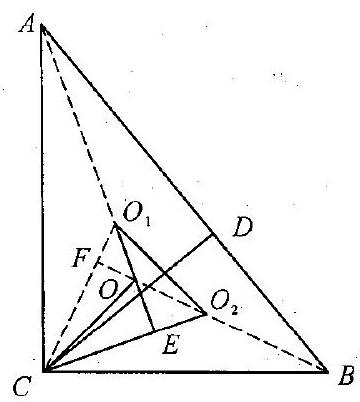
\includegraphics[max width=\textwidth, center]{2024_10_30_2c8f45efd4a519b08e1ag-034(2)}

图3-16

又 $\angle C E O=\angle O_{2} E O_{1}=90^{\circ}$, 故 Rt $\triangle C E O \cong$ Rt $\triangle O_{1} E O_{2}$.\\
所以 $C O=O_{1} O_{2}$.\\
例13 如图 3-17, $\triangle A B C$ 是等腰直角三角形, $\angle C=90^{\circ}$, 点 $M 、 N$ 分别是边 $A C$ 和 $B C$ 的中点, 点 $D$ 在射线 $B M$ 上,且 $B D=2 B M$ 。点 $E$ 在射线 $N A$ 上,且 $N E=2 N A$ ,求证: $B D \perp D E$ 。(1996年天津市竞赛题)

证明 连 $A D$, 取 $A D$ 的中点 $F$, 连 $E F$ 。由 $A C=B C, C N=C M$ ,知 $\mathrm{Rt} \triangle A C N \cong$ $\mathrm{Rt} \triangle B C M$, 则 $\angle N A C=\angle M B C$, 即 $\angle 3=\angle 6$.

由 $B M=D M, C M=A M, \angle B M C=$ $\angle A M D$ ,知 $\triangle B C M \cong \triangle D A M$ ,则 $A D=B C$ ,且\\
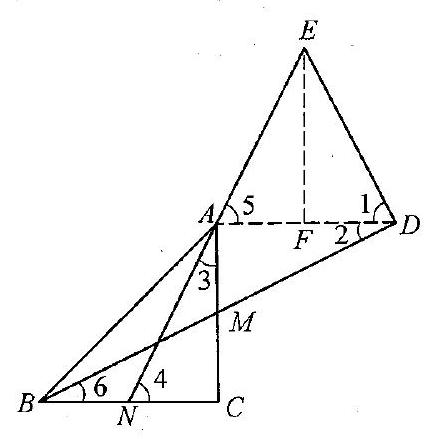
\includegraphics[max width=\textwidth, center]{2024_10_30_2c8f45efd4a519b08e1ag-034}

图3-17\\
$\angle A D M=\angle M B C$ ,即 $\angle 2=\angle 6$ 。故 $\angle A D M=$ $\angle C A N$, 且 $A D / / B C$, 即 $\angle 2=\angle 3$ 且 $\angle 4=\angle 5$.

又由 $A E=A N, \angle A N C=\angle E A F, A F=N C$, 知 $\triangle A E F \cong \triangle N A C$,则 $\angle E F A=\angle C=90^{\circ}$ 。

因 $A F=F D$ ,则 $\angle E D F=\angle E A F=\angle A N C ,$ 而 $\angle N A C+\angle A N C=$ $90^{\circ}$, 故 $\angle E D F+\angle A D M=90^{\circ}$, 即 $B D \perp D E$ 。\\
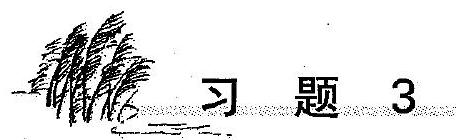
\includegraphics[max width=\textwidth, center]{2024_10_30_2c8f45efd4a519b08e1ag-034(1)}\\
$11 \triangle A B C$ 的 $\angle A$ 的平分线为 $A D, M$ 为 $B C$ 的中点, 又 $M E / / A D$ 交 $A C$ 于 $F$ ,交 $B A$ 的延长线于 $E$ 。求证: $B E=C F=\frac{1}{2}(A B+A C)$ 。(1994 年天津市竞赛题)

2 . 已知: 五边形 $A B C D E$ 中, $\angle A B C=\angle A E D=90^{\circ}, \angle B A C=\angle E A D$, $M$ 为 $C D$ 的中点. 求证: $M B=M E$ 。(1991 年太原市竞赛题)\\
3 在梯形 $A B C D$ 中,腰 $A B=C D$ ,将 $\triangle A B C$ 绕点 $C$ 转过一个角度,而得到 $\triangle A^{\prime} B^{\prime} C$. 求证: $A^{\prime} D 、 B C$ 和 $B^{\prime} C$ 的中点共线。(第 23 届全俄奥林匹克题)\\
4 以 $\triangle A B C$ 的边 $A B 、 A C$ 为斜边向外作直角三角形 $A B D$ 和 $A C E$ ,且使 $\angle A B D=\angle A C E, M$ 是 $B C$ 的中点。求证: $D M=E M$ 。(第 10 届"祖冲之"杯邀请赛题)\\
5 给定凸四边形 $A B C D$ 与形内一点 $O$, 且 $\angle A O B=\angle C O D=120^{\circ}, A O=$ $O B, C O=O D$. 设 $K 、 L 、 M$ 分别为线段 $A B 、 B C 、 C D$ 的中点. 证明:\\
(1) $K L=L M$ ;\\
(2) $\triangle K L M$ 为等边三角形。\\
(第58届莫斯科奥林匹克题)\\
6. $\triangle D E F$ 是将 $\triangle A B C$ 沿边 $B C$ 平移得到的,且 $D E$ 经过 $A C$ 的中点 $M$. 求证: $M$ 是 $D E$ 的中点。\\
7. 7 在等腰 $\triangle A B C$ 中, 顶角 $\angle B A C=100^{\circ}$, 延长 $A B$ 到 $D$, 使 $A D=B C$, 求 $\angle B C D$ 的度数。\\
8 在等腰直角 $\triangle A B C$ 中, $\angle C=90^{\circ}, A M$ 是 $B C$ 边上的中线, $C N \perp A M$ 交 $A B$ 于 $N$ ,求证: $\angle N M B=\angle C M A$ 。\\
9 在等腰直角 $\triangle A B C$ 的斜边 $A B$ 上取两点 $M 、 N$, 使 $\angle M C N=45^{\circ}$. 记 $A M=m, M N=l, B N=n$ ,以 $l 、 m 、 n$ 为边长作三角形,试问:此三角形有什么特点?\\
10. 已知凸五边形 $A B C D E$ 中, $\angle A B C=\angle A E D=90^{\circ}, \angle D A C=30^{\circ}$, $\angle B A E=70^{\circ}, F$ 是边 $C D$ 的中点, 且 $F B=F E$ 。求 $\angle B A C$ 的度数.\\
111 如图,设 $D$ 为等边 $\triangle A B C$ 内一点, $D B=D A$ , $B F=A B, \angle D B F=\angle D B C$ 。 求 $\angle B F D$ 的度数。\\
12 在 $\triangle A B C$ 中, $A C=B C, \angle A C B=90^{\circ}, D$ 是 $A C$ 上一点, 且 $A E$ 垂直 $B D$ 的延长线于 $E$, 又 $A E=$ $\frac{1}{2} B D$ 。求证: $B D$ 是 $\angle A B C$ 的平分线。(1990年北京市竞赛题)\\
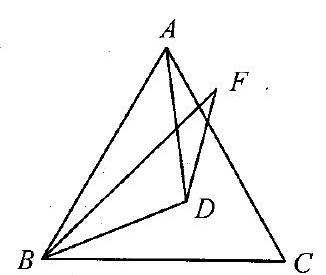
\includegraphics[max width=\textwidth, center]{2024_10_30_2c8f45efd4a519b08e1ag-035}\\
(第 11 题)\\
$13 \triangle \triangle A B C$ 中, $\angle C=90^{\circ}, D$ 为 $A B$ 上一点, 作 $D E \perp B C$ 于 $E$, 使 $B E=A C$, 且 $B D=\frac{1}{2}$, 又 $D E+B C=1$. 求证: $\angle A B C=30^{\circ}$ 。(1990 年"汉江杯"竞赛题)\\
14 锐角 $\triangle A B C$ 的高 $A A_{1}$ 和 $C C_{1}$ 相交于点 $O$. 求证: 如果 $O A=O C$, 那么 $\triangle A B C$ 是等腰三角形。(第20届全俄奥林匹克题)

对应角相等、对应边成比例的三角形,叫做相似三角形。\\
相似三角形对应边的比,叫做相似比(或相似系数)。\\
判定三角形相似的方法,有\\
定理1 平行于三角形一边的直线和其他两边(或两边的延长线)相交,所构成的三角形与原三角形相似。

定理2 如果一个直角三角形的斜边和一条直角边与另一个直角三角形的斜边和一条直角边对应成比例,那么这两个三角形相似。

判定定理1 如果一个三角形的两个角与另一个三角形的两个角对应相等,那么这两个三角形相似。

判定定理2 如果一个三角形的两条边与另一个三角形的两条边对应成比例,且对应夹角相等,那么这两个三角形相似。

判定定理3 如果一个三角形的三条边与另一个三角形的三条边对应成比例,那么这两个三角形相似。

直角三角形有一个特殊的角一一直角,因而对于一般的相似三角形的判定方法中,现在已经确定了一个角对应相等,只需再寻求其余一个条件,即可判定两个直角三角形相似。

相似三角形有如下重要性质:\\
相似三角形的对应角相等,对应边成比例。\\
相似三角形的对应边上的重要线段(如中线、高等)成比例,且等于相似比;对应角的平分线成比例,且等于相似比。

相似三角形的面积的比等于相似比的平方。\\
研究比例线段是研究相似三角形的一个重要内容。\\
比例线段产生的途径主要有:\\
(1)平行线截割 平行线有一个重要性质:过一点三条直线截两条平行直线,截得的线段对应成比例;\\
(2)角平分线性质定理;\\
(3)面积比式(包括后面的共边比例定理,共角比例定理);\\
(4)线段等积式变形(包括后面的梅涅劳斯定理、塞瓦定理)。\\
在讨论有关比例线段时,还要注意比例定理的灵活运用。\\
例1 如图 4-1, $P$ 为 $\triangle A B C$ 内任一点, 过 $P$作 $A D 、 B E 、 C F$ 分别与 $B C 、 A C 、 A B$ 交于 $D$ 、 $E 、 F$ 。\\
求证: (1) $\frac{P D}{A D}+\frac{P E}{B E}+\frac{P F}{C F}=1$ ;\\
(2) $\frac{A P}{A D}+\frac{B P}{B E}+\frac{C P}{C F}=2$.\\
证明(1)过 $P$ 作 $M N / / B C$ 交 $A B 、 A C$ 于\\
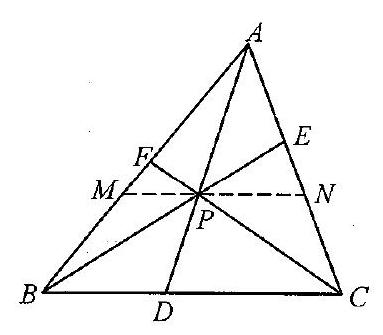
\includegraphics[max width=\textwidth, center]{2024_10_30_2c8f45efd4a519b08e1ag-037}

图 4-1\\
$M 、 N$ ,则

\begin{align*}
\frac{A P}{A D}=\frac{M P}{B D}=\frac{P N}{D C}=\frac{M P+P N}{B D+D C}=\frac{M N}{B C}
\end{align*}

由分比性质,有

\begin{align*}
\frac{P D}{A D}=\frac{B C-M N}{B C}
\end{align*}

又由 $M N / / B C$ ,有

故

\begin{align*}
\frac{P E}{B E}=\frac{P N}{B C}, \frac{P F}{F C}=\frac{P M}{B C}
\end{align*}

\begin{align*}
\frac{P D}{A D}+\frac{P E}{B E}+\frac{P F}{C F}=\frac{B C-M N}{B C}+\frac{P N}{B C}+\frac{P M}{B C}=1
\end{align*}

另证 转换为面积比,有

\begin{align*}
\frac{P D}{A D}+\frac{P E}{B E}+\frac{P F}{C F}=\frac{S_{\triangle P B C}}{S_{\triangle A B C}}+\frac{S_{\triangle P A C}}{S_{\triangle A B C}}+\frac{S_{\triangle P A B}}{S_{\triangle A B C}}=\frac{S_{\triangle A B C}}{S_{\triangle A B C}}=1
\end{align*}

(2)由

\begin{align*}
\frac{A P}{A D}=\frac{A D-P D}{A D}=\frac{S_{\triangle A B C}-S_{\triangle P B C}}{S_{\triangle A B C}}
\end{align*}

及

\begin{align*}
\begin{gathered}
\frac{B P}{B E}=\frac{S_{\triangle A B C}-S_{\triangle P A C}}{S_{\triangle A B C}}, \frac{C P}{C F}=\frac{S_{\triangle A B C}-S_{\triangle P A B}}{S_{\triangle A B C}} \\
\frac{A P}{A D}+\frac{B P}{B E}+\frac{C P}{C F}=\frac{3 S_{\triangle A B C}-S_{\triangle P B C}-S_{\triangle P A C}-S_{\triangle P A B}}{S_{\triangle A B C}}=2
\end{gathered}
\end{align*}

例2 如图 4-2, $H$ 是 $\triangle A B C$ 的高 $A D$ 上的任一点, $B H 、 C H$ 分别交 $A C 、 A B$ 于 $E 、 F$ 。求证: $\angle E D H=\angle F D H$ 。(1985 年扬州市竞赛题,第 26 届加拿大奥林匹克题)\\
得

\section*{厦门郑剑雄高中数学竞赛系列}
全国小学奥数群:221739457,全国初中奥数学生群:253736211,全国高中奥数学生群591782992全国初中奥数教练群112464128,全国高中奥数教练群195949359竞赛公众号:新浪微博@郑剑雄 微信:v136257437 QQ:136257437\\
业务:初高中联赛班、培优班、美国高中数学、教师培训、机构教学产品研发、讲义资料出售等

又 $\angle B A C=180^{\circ}-\beta-\gamma, \angle A B C=180^{\circ}-\alpha-\gamma, \angle A C B=180^{\circ}-\alpha-$ $\beta$, 则 $\angle B A C+\angle A B C+\angle A C B=540^{\circ}-2(\alpha+\beta+\gamma)=180^{\circ}$ ,即 $\alpha+\beta+$ $\gamma=180^{\circ}$ ,从而,推知 $\angle B A C=\alpha, \angle A B C=\beta, \angle A C B=\gamma$ 。故\\
$\triangle D E C \backsim \triangle A E F \backsim \triangle D B F$.\\
例 5 如图 4-5,在 $\triangle A B C$ 中, $A B=A C$ , $D$ 是底边上一点, $E$ 是线段 $A D$ 上一点, 且 $\angle B E D=$ $2 \angle C E D=\angle B A C$ 。求证: $B D=2 C D$ 。(1992 年全国联赛题,同§3中例4)

证明 过 $D$ 作 $D F / / C A$ 交 $A B$ 于 $F$ ,在 $B D$ 上取点 $G$ ,使 $B G=D C$ ,连结 $A G 、 F G$ 。

由 $D F / / C A$, 有 $\angle B F D=\angle B A C, F B=F D$ 。\\
又 $A B=A C, \angle A B G=\angle A C D, B G=D C$ ,知\\
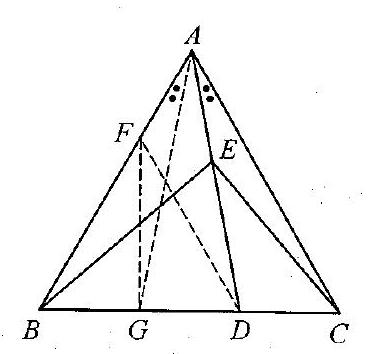
\includegraphics[max width=\textwidth, center]{2024_10_30_2c8f45efd4a519b08e1ag-039(1)}

图4-5\\
$\triangle A B G \cong \triangle A C D$. 于是, $A G=A D, \angle F A G=\angle E A C$.

而 $\angle A B E=\angle B E D-\angle B A E=\angle B A C-\angle B A E=\angle E A C=\angle F D A$,注意到 $\angle B A E$ 公用, 则 $\triangle A B E \backsim \triangle A D F$, 即有 $\frac{A E}{A B}=\frac{A F}{A D}$, 从而 $\frac{A F}{A G}=\frac{A E}{A C}$.

又 $\angle F A G=\angle E A C$, 故 $\triangle F A G \backsim \triangle E A C$, 有 $\angle A F G=\angle A E C$. 从而 $\angle B F G=\angle D E C=\frac{1}{2} \angle B E D=\frac{1}{2} \angle B A C=\frac{1}{2} \angle B F D$ ,则 $\triangle B F G \cong$ $\triangle D F G$. 即有 $B G=G D$, 故 $B D=2 C D$.

例 6 锐角 $\triangle A B C$ 的三条高 $A A_{1} 、 B B_{1} 、 C C_{1}$的中点分别为 $A_{2} 、 B_{2} 、 C_{2}$ 。试求 $\angle B_{2} A_{1} C_{2}+$ $\angle C_{2} B_{1} A_{2}+\angle A_{2} C_{1} B_{2}$ 。(第 22 届全俄奥林匹克题)

解 先求 $\angle B_{2} A_{1} C_{2}$. 连 $A_{1} B_{1} 、 A_{1} C_{1}$, 延长 $A_{1} B_{2}$ 至 $B^{\prime}{ }_{2}$ ,使 $B^{\prime}{ }_{2} B_{2}=A_{1} B_{2}$ ,延长 $A_{1} C_{2}$ 至 $C_{2}^{\prime}$ ,使 $C^{\prime}{ }_{2} C_{2}=A_{1} C_{2}$ 。连 $C_{1} C^{\prime}{ }_{2} 、 B_{2}^{\prime}{ }_{2}$ ,则

\begin{align*}
\begin{aligned}
& \triangle C^{\prime}{ }_{2} C_{1} C_{2} \cong \triangle A_{1} C C_{2} \\
& \triangle B^{\prime}{ }_{2} B_{1} B_{2} \cong \triangle A_{1} B B_{2}
\end{aligned}
\end{align*}

\begin{center}
\includegraphics[max width=\textwidth]{2024_10_30_2c8f45efd4a519b08e1ag-039}
\end{center}

图 4-6

因此

\begin{align*}
\begin{aligned}
& \angle C_{2}^{\prime} C_{1} A_{1}=\angle C_{1} A_{1} B \stackrel{(*)}{=} \angle B_{1} A_{1} C \stackrel{(* *)}{=} \angle A \\
& \angle B_{2}^{\prime} B_{1} A_{1}=\angle B_{1} A_{1} C, B_{1} B_{2}^{\prime}=A_{1} B, C_{1} C_{2}^{\prime}=A_{1} C .
\end{aligned}
\end{align*}

其中(*)由本节中例2的结论即得, $(* *)$ 由本节中例 4 的结论即得。\\
又由本节中例 4 的结论,有 $\triangle B A_{1} C_{1} \backsim \triangle B_{1} A_{1} C$ ,因此

\begin{align*}
\frac{B A_{1}}{C_{1} A_{1}}=\frac{B_{1} A_{1}}{C A_{1}} \text {, 即 } \frac{C_{1} C_{2}^{\prime}}{C_{1} A_{1}}=\frac{B_{1} A_{1}}{B_{1} B_{2}^{\prime}} \text {. }
\end{align*}

注意到 $\angle A_{1} C_{1} C_{2}^{\prime}=\angle A_{1} B_{1} B_{2}^{\prime}$, 故 $\triangle C_{1} A_{1} C_{2}^{\prime} \backsim \triangle B_{1} B_{2}^{\prime} A_{1}$. 即有 $\angle C_{2} A_{1} C_{1}=$ $\angle A_{1} B_{2}^{\prime} B_{1}$ 。于是,

\begin{align*}
\begin{aligned}
\angle B_{2} A_{1} C_{2} & =\angle B_{2} A_{1} B_{1}+\angle C_{2} A_{1} C_{1}-\angle B_{1} A_{1} C_{1} \\
& =\angle B_{2} A_{1} B_{1}+\angle A_{1} B_{2}{ }_{2} B_{1}-\left(180^{\circ}-2 \angle A\right) \\
& =\left(180^{\circ}-\angle A\right)-\left(180^{\circ}-2 \angle A\right)=\angle A .
\end{aligned}
\end{align*}

同理,

\begin{align*}
\angle C_{2} B_{1} A_{2}=\angle B, \angle A_{2} C_{1} B_{2}=\angle C .
\end{align*}

故

\begin{align*}
\angle B_{2} A_{1} C_{2}+\angle C_{2} B_{1} A_{2}+\angle A_{2} C_{1} B_{2}=180^{\circ}
\end{align*}

例7 如图 4-7, $P$ 是 $\triangle A B C$ 内一点, 过 $P$ 分别作直线平行于 $\triangle A B C$ 的各边,所成的小三角形 $t_{1} 、 t_{2}$ 和 $t_{3}$ 的面积分别是 $4 、 9$ 和 49 。 求 $\triangle A B C$ 的面积。(第2届美国邀请赛题)

解 如图 4-7, 设点 $R 、 T$ 在 $A B$ 上, $N 、 E$ 在 $B C$ 上, $D 、 M$ 在 $A C$ 上, 且 $M N / / A B, T D / / B C$, $R E / / A C$ ,则\\
\includegraphics[max width=\textwidth, center]{2024_10_30_2c8f45efd4a519b08e1ag-040}

图 4-7.\\
$\triangle P E N \backsim \triangle M C N \backsim \triangle M D P \backsim \triangle A D T \backsim \triangle R P T \backsim \triangle A B C$.\\
设 $M P=p, P N=q, R T=r, A B=c, S_{\triangle A B C}=S$, 则

即

\begin{align*}
\begin{gathered}
p+q+r=c, \frac{4}{S}=\frac{q^{2}}{c^{2}}, \frac{9}{S}=\frac{p^{2}}{c^{2}}, \frac{49}{S}=\frac{r^{2}}{c^{2}} . \\
\frac{2}{\sqrt{S}}=\frac{q}{c}, \frac{3}{\sqrt{S}}=\frac{p}{c}, \frac{7}{\sqrt{S}}=\frac{r}{c} .
\end{gathered}
\end{align*}

以上三式相加,得

故

\begin{align*}
\begin{gathered}
\frac{2+3+7}{\sqrt{S}}=\frac{p+q+r}{c}=1 \\
S_{\triangle A B C}=S=(2+3+7)^{2}=144
\end{gathered}
\end{align*}

例8 如图 4-8, $\triangle U V W$ 与 $\triangle X Y Z$ 的边分别交于 $A 、 B 、 C 、 D 、 E 、 F$.若 $\frac{A B}{U V}=\frac{C D}{V W}=\frac{E F}{W U}$. 求证: $\frac{B C}{X Y}=\frac{D E}{Y Z}=\frac{F A}{Z X}$ 。(2003 年武汉市竞赛题)

证明 过点 $A 、 B$ 分别作 $U W 、 W V$ 的平行线, 交点为 $P$. 连 $P E 、 P D$, 则

\section*{夏门郑剑雄高中数学竞赛系列}
全国小学奥数群:221739457,全国初中奥数学生群:253736211,全国高中奥数学生群591782992全国初中奥数教练群112464128,全国高中奥数教练群195949359竞赛公众号:新浪微博@郑剑雄 微信:v136257437 QQ: 136257437\\
业务:初高中联赛班、培优班、美国高中数学、教师培训、机构教学产品研发、讲义资料出售等

\begin{align*}
\triangle A B P \backsim \triangle U V W .
\end{align*}

从而

\begin{align*}
\frac{A B}{U V}=\frac{B P}{V W}=\frac{P A}{W U}
\end{align*}

由题设 $\frac{A B}{U V}=\frac{C D}{V W}=\frac{E F}{W U}$, 知

\begin{align*}
C D=B P, \quad E F=P A
\end{align*}

\begin{center}
\includegraphics[max width=\textwidth]{2024_10_30_2c8f45efd4a519b08e1ag-041(1)}
\end{center}

图 4-8

从而\\
$C D \cong B P, E F \Perp P A$.\\
连 $P C 、 P F$ ,则由 $\triangle B P C \cong \triangle D C P, \triangle A F P \cong \triangle E P F$ ,知 $B C \cong P D$ , $F A \underline{I} E P$ (亦可直接由平行四边形性质得到),于是

\section*{$\triangle P D E \backsim \triangle X Y Z$.}
因此

\begin{align*}
\begin{aligned}
& \frac{P D}{X Y}=\frac{D E}{Y Z}=\frac{E P}{Z X} . \\
& \frac{B C}{X Y}=\frac{D E}{Y Z}=\frac{F A}{Z X} .
\end{aligned}
\end{align*}

例 9 如图 4-9, 已知 $P$ 为 Rt $\triangle A B C$ 的斜边 $B C$ 上一点, $Q$ 为 $P C$ 的中点,过 $P$ 作 $B C$ 的垂线,交 $A B$ 于 $R, H$ 为 $A R$ 的中点,过 $H$ 向 $C$ 所在一侧作射线 $H N \perp A B$ 。证明:射线 $H N$ 上存在一点 $G$ ,使 $A G=C Q , B G=B Q$ 。(2002 年全国联赛题)\\
\includegraphics[max width=\textwidth, center]{2024_10_30_2c8f45efd4a519b08e1ag-041}

图4-9

证明 首先由 $B C>A B, B R>B P$, 则

\begin{align*}
A H=\frac{1}{2}(A B-B R)<\frac{1}{2}(B C-B P)=C Q
\end{align*}

于是,以 $A$ 为圆心, $C Q$ 为半径画圆弧必交 $N H$ 上一点 $G$ ,且有 $A G=C Q$ 。\\
连 $B G$ ,因 $\angle B A C=\angle B P R=90^{\circ}, \angle B$ 公用,则

所以

\begin{align*}
\mathrm{Rt} \triangle B P R \backsim \mathrm{Rt} \triangle B A C
\end{align*}

又 $C Q=Q P, A H=H R$, 所以上式即为

\begin{align*}
(B H-A H)(B H+A H)=(B Q-C Q)(B Q+C Q),
\end{align*}

即

\begin{align*}
B H^{2}-A H^{2}=B Q^{2}-C Q^{2}
\end{align*}

而

\begin{align*}
C Q^{2}=A G^{2}=A H^{2}+H G^{2}
\end{align*}

\section*{夏门郑剑雄高中数学竞赛系列}
全国小学奥数群:221739457,全国初中奥数学生群:253736211,全国高中奥数学生群591782992全国初中奥数教练群112464128,全国高中奥数教练群195949359竞赛公众号:新浪微博@郑剑雄 微信:v136257437 QQ: 136257437\\
业务:初高中联赛班、培优班、美国高中数学、教师培训、机构教学产品研发、讲义资料出售等

则

\begin{align*}
B H^{2}=B Q^{2}-\left(C Q^{2}-A H^{2}\right)=B Q^{2}-H G^{2},
\end{align*}

即

\begin{align*}
B G^{2}=B H^{2}+H G^{2}=B Q^{2}
\end{align*}

故

\begin{align*}
B G=B Q .
\end{align*}

所以在 $H N$ 上存在一点 $G$, 使 $A G=C Q, B G=B Q$.\\
例10 如图 4-10, $A D$ 是锐角 $\triangle A B C$ 边 $B C$ 上的高, $E$ 是 $A D$ 上的一点且满足 $\frac{A E}{E D}=\frac{C D}{D B}$ ,过 $D$ 作 $D F \perp B E$ 于 $F$ 。求证: $\angle A F C=90^{\circ}$ 。(1999 年上海中学数学实验班选拔赛题)

证明 因 $D F$ 为 $\mathrm{Rt} \triangle B D E$ 斜边 $B E$ 上的高,则 $\angle E D F=\angle F B D$ ,从而

\begin{align*}
\mathrm{Rt} \triangle E F D \backsim \mathrm{Rt} \triangle D F B, \frac{E D}{E F}=\frac{D B}{D F}
\end{align*}

所以

\begin{align*}
\frac{A E}{E F}=\frac{A E}{E D} \cdot \frac{E D}{E F}=\frac{A E}{E D} \cdot \frac{D B}{D F}
\end{align*}

\begin{center}
\includegraphics[max width=\textwidth]{2024_10_30_2c8f45efd4a519b08e1ag-042}
\end{center}

图 4-10

由题设 $\frac{A E}{E D}=\frac{C D}{D B}$ ,所以

\begin{align*}
\frac{A E}{E F}=\frac{C D}{D B} \cdot \frac{D B}{D F}
\end{align*}

即

\begin{align*}
\frac{A E}{E F}=\frac{C D}{D F} \tag{1}
\end{align*}

又

\begin{align*}
\angle A E F=90^{\circ}+\angle E D F=\angle C D F \tag{2}
\end{align*}

由(1)、(2)知 $\triangle A E F \backsim \triangle C D F, \angle A F E=\angle C F D$,\\
故

\begin{align*}
\angle A F C=\angle D F E=90^{\circ} .
\end{align*}

例11 如图 4-11, $A D$ 是 Rt $\triangle A B C$ 斜边 $B C$ 上的高, $P$ 是 $A D$ 的中点,连结 $B P$ 并延长交 $A C$ 于 $E$ 。已知 $A C: A B=k$ 。求 $A E: E C$ 。(1999年山东省竟赛题)

解 由题设,注意到 $\angle A B C$ 或 $\angle C$ 公用,则\\
$\mathrm{Rt} \triangle B D A \backsim \mathrm{Rt} \triangle B A C \backsim \mathrm{Rt} \triangle A D C$,\\
\includegraphics[max width=\textwidth, center]{2024_10_30_2c8f45efd4a519b08e1ag-042(1)}

图 4-11

得

\begin{align*}
\frac{A D}{B D}=\frac{A C}{A B}=\frac{D \dot{C}}{A D}=k
\end{align*}

令 $B D=a$, 则 $A D=k a, D C=k^{2} a$. 从而,

\begin{align*}
\frac{D C}{B D}=\frac{k^{2} a}{a}=k^{2}, \frac{B C}{B D}=\frac{D C+B D}{B D}=1+k^{2}
\end{align*}

延长 $B E$ 到 $F$, 使 $A F / / B C$ ,则

\begin{align*}
\triangle A E F \backsim \triangle C E B, \text { 从而 } \frac{A E}{E C}=\frac{A F}{B C} \text {. }
\end{align*}

在 Rt $\triangle A F P$ 和 Rt $\triangle D B P$ 中, 因 $A P=P D, \angle A P F=\angle D P B$, 所以

\begin{align*}
\text { Rt } \triangle A F P \cong \mathrm{Rt} \triangle D B P \text {, 即有 } A F=B D \text {. }
\end{align*}

故

\begin{align*}
\frac{A E}{E C}=\frac{A F}{B C}=\frac{B D}{B C}=\frac{1}{1+k^{2}}
\end{align*}

\begin{center}
\includegraphics[max width=\textwidth]{2024_10_30_2c8f45efd4a519b08e1ag-043(1)}
\end{center}

I 设 $M 、 N$ 为三角形 $A B C$ 的边 $B C$ 上的两点,且满足 $B M=M N=N C$ ,一平行于 $A C$ 的直线分别交 $A B 、 A M 、 A N$ 于 $D 、 E 、 F$ 。求证: $E F=3 D E$ 。 (1994 年澳大利亚奥林匹克题)\\
2 已知:在 $\triangle A B C$ 中, $A^{\prime} 、 B^{\prime} 、 C^{\prime}$ 分别在 $B C 、 A C$ 和 $A B$ 上, $A A^{\prime} 、 B B^{\prime}$ 和 $C C^{\prime}$ 相交于一点 $O$ ,并且 $\frac{A O}{O A^{\prime}}+\frac{B O}{O B^{\prime}}+\frac{C O}{O C^{\prime}}=92$ 。试求 $\frac{A O}{O A^{\prime}} \cdot \frac{B O}{O B^{\prime}} \cdot \frac{C O}{O C^{\prime}}$的值。(第10届美国邀请赛题)\\
3 令 $P$ 是 $\triangle A B C$ 的一个内点,延长 $A P 、 B P 、 C P$与对边相交如图。图中 $a 、 b 、 c 、 d$ 为各线段之长。已知: $a+b+c=43, d=3$ 。求 $a b c$ 的值。 (第6届美国邀请赛题)\\
4 在 $\triangle A B C$ 中, 设 $l$ 是经过顶点 $C$ 且与 $A B$ 平行的一条直线, $\angle A$ 的平分线与边 $B C$ 交于 $D$ ,与 $l$\\
\includegraphics[max width=\textwidth, center]{2024_10_30_2c8f45efd4a519b08e1ag-043}\\
(第3题)

交于 $E . \angle B$ 的平分线与边 $A C$ 交于 $F$ ,与 $l$ 交于 $G$ 。若 $G F=D E$ ,求证: $A C=B C$.\\
55 等腰 $\triangle A B C$ 的顶角 $\angle A=108^{\circ}, B C=m, A B=A C=n$. 记 $x=\frac{m+n}{m-n}$, $y=\frac{(m+n)^{2}}{m n}, z=\frac{m^{3}}{n^{3}}$. 试排出 $x 、 y 、 z$ 的大小关系。\\
6. 在 $\triangle A B C$ 中, $A D$ 是 $\angle B A C$ 的平分线, 若 $A B+B D=25, A C-C D=4$,求 $A D$ 之长.

\section*{厦门郑剑雄高中数学竞赛系列}
全国小学奥数群:221739457,全国初中奥数学生群:253736211,全国高中奥数学生群591782992全国初中奥数教练群112464128,全国高中奥数教练群195949359竞赛公众号:新浪微博@郑剑雄 微信:v136257437 QQ:136257437\\
业务:初高中联赛班、培优班、美国高中数学、教师培训、机构教学产品研发、讲义资料出售等

7 已知正五边形的周长等于 $p$, 所有对角线的长度之和等于 $q$, 求 $\frac{q}{p}-\frac{p}{q}$的值。\\
8 设 $O$ 是 $\triangle A B C$ 内任一点, 直线 $A O 、 B O 、 C O$ 分别与三边相交于 $P 、 Q$ 、 $R$. 令 $B C=a, C A=b, A B=c$. 若 $a>b>c$, 求证: $O P+O Q+$ $O R<a$.\\
9 等腰三角形 $A B C$ 中, $\angle A=100^{\circ}, A B=A C$ ,角 $B$ 的平分线交 $A C$ 于 $D$ 。求证: $B D+A D=B C$ 。(第 23 届加拿大奥林匹克训练题)\\
10 在 $\triangle A B C$ 中, 若 $\angle A=2 \angle B$, 边 $A C=4, A B=5$, 则边 $B C$ 等于 ( ).\\
A. 6\\
B. 7\\
C. $3 \sqrt{5}$\\
D. 5\\
(1997 年陕西省竞赛题)\\
11 如图, $\triangle A B C$ 和 $\triangle A_{1} B_{1} C_{1}$ 均为正三角形, $B C$ 和 $B_{1} C_{1}$ 的中点均为 $D$ 。求证: $A A_{1} \perp C C_{1}$. (2000 年重庆市竞赛题)\\
\includegraphics[max width=\textwidth, center]{2024_10_30_2c8f45efd4a519b08e1ag-044(1)}\\
(第11题)\\
\includegraphics[max width=\textwidth, center]{2024_10_30_2c8f45efd4a519b08e1ag-044}\\
(第 12 题)

12 如图, 大正方形 $A B C D$ 及小正方形 $A E F G$ 共顶点 $A$, 连 $B E 、 C F 、 D G$, 求 $B E : C F : D G$ 。\\
13 在 $\triangle A B C$ 中, $B C=2 A C, D 、 E$ 分别是边 $B C 、 A B$ 上的点, 且 $\angle B=$ $\angle E D A=\angle D A C$ 。如果 $\triangle A B C 、 \triangle E B D 、 \triangle A D C$ 的周长依次为 $m 、 m_{1}$ 、 $m_{2}$ 。求证: $5 m=4\left(m_{1}+m_{2}\right)$ 。\\
14 在 $\triangle A B C$ 的与边 $B C$ 平行的中位线 $M N$ 上任取一点 $P$, 射线 $B P 、 C P$ 分别交 $A C 、 A B$ 于 $F 、 E$ 。试证: $\frac{A E}{E B}+\frac{A E}{F C}=1$ 。\\
15 在正 $\triangle A B C$ 的边 $B C 、 C A$ 上各有一点 $E 、 F, B E=C F=a, E C=F A=$ b. 当 $B F$ 平分 $A E$ 时,试比较 $\frac{2 a+b}{b} 、 \frac{a+b}{a-b} 、 \frac{(a+b)^{2}}{a b} 、 \frac{a^{3}}{b^{3}}$. 的大小.

16 在 $\triangle A B C$ 中, $\angle A C B=90^{\circ}, A C=B C, D$ 是 $B C$ 延长线上的一点, $B E \perp A D$ 于 $E, B E$ 与 $A C$ 交于点 $F$. 求证: $C D=C F$ 及 $D E>D C$ 。(1994

\section*{夏门郑剑雄高中数学竞赛系列}
全国小学奥数群:221739457,全国初中奥数学生群:253736211,全国高中奥数学生群591782992全国初中奥数教练群112464128,全国高中奥数教练群195949359竞赛公众号:新浪微博@郑剑雄 微信:v136257437 QQ:136257437\\
业务:初高中联赛班、培优班、美国高中数学、教师培训、机构教学产品研发、讲义资料出售等年四川省竞赛题)\\
17 在 $\triangle A B C$ 中, $B C=a, A C=b, A B=c, \angle C=90^{\circ}, C D$ 和 $B E$ 是 $\triangle A B C$ 的两条中线,且 $C D \perp B E$ 。求 $a: b: c$ 。(1997 年安徽省部分地区竞赛题)\\
$18 \triangle A B C$ 中, $A B=2, A C=\sqrt{3}, \angle A=\angle B C D=45^{\circ}$ ( $D$ 在 $A B$ 的延长线上)。求 $B C$ 及 $\triangle B D C$ 的面积. (1997 年山东省竞赛题)

19 在 $\triangle A B C$ 中, $A B=A C, B C$ 上的高 $A D=5, M$ 为 $A D$ 上一点, $M D=1$ ,且 $\angle B M C=3 \angle B A C$ 。试求 $\triangle A B C$ 的周长。(1995 年四川省竟赛题)

\section*{三角形中与比例线段有关的}
\section*{几个定理}
梅涅劳斯定理 设 $A^{\prime} 、 B^{\prime} 、 C^{\prime}$ 分别是 $\triangle A B C$ 的三边 $B C 、 C A 、 A B$ 或其延长线上的点, 若 $A^{\prime} 、 B^{\prime} 、 C^{\prime}$ 三点在一条直线上, 则

\begin{align*}
\frac{B A^{\prime}}{A^{\prime} C} \cdot \frac{C B^{\prime}}{B^{\prime} A} \cdot \frac{A C^{\prime}}{C^{\prime} B}=1 \tag{5-1}
\end{align*}

注 若采用有向线段,上式右边为 -1 (下面均同)。

证明 如图 5-1, 过 $A$ 作直线 $A D / / C^{\prime} A^{\prime}$ ,交 $B C$ 的延长线于 $D$ ,则

\begin{align*}
\frac{C B^{\prime}}{B^{\prime} A}=\frac{C A^{\prime}}{A^{\prime} D}, \frac{A C^{\prime}}{C^{\prime} B}=\frac{D A^{\prime}}{A^{\prime} B}
\end{align*}

\begin{center}
\includegraphics[max width=\textwidth]{2024_10_30_2c8f45efd4a519b08e1ag-046}
\end{center}

图5-1

故

\begin{align*}
\frac{B A^{\prime}}{A^{\prime} C} \cdot \frac{C B^{\prime}}{B^{\prime} A} \cdot \frac{A C^{\prime}}{C^{\prime} B}=\frac{B A^{\prime}}{A^{\prime} C} \cdot \frac{C A^{\prime}}{A^{\prime} D} \cdot \frac{D A^{\prime}}{A^{\prime} \bar{B}}=1
\end{align*}

梅涅劳斯定理的逆定理 设 $A^{\prime} 、 B^{\prime} 、 C^{\prime}$ 分别是 $\triangle A B C$ 的三边 $B C 、 C A$ 、 $A B$ 或其延长线上的点且其中仅一点在延长线上或三点均在延长线上,若

\begin{align*}
\frac{B A^{\prime}}{A^{\prime} C} \cdot \frac{C B^{\prime}}{B^{\prime} A} \cdot \frac{A C^{\prime}}{C^{\prime} B}=1 \tag{5-2}
\end{align*}

则 $A^{\prime} 、 B^{\prime} 、 C^{\prime}$ 三点在一条直线上.\\
证明 不妨设仅有点 $A^{\prime}$ 在 $B C$ 的延长线上, 则直线 $A^{\prime} B^{\prime}$ 与边 $A B$ 相交,设交点为 $C_{1}$ ,由梅涅劳斯定理,得到

\begin{align*}
\begin{aligned}
& \frac{B A^{\prime}}{A^{\prime} C} \cdot \frac{C B^{\prime}}{B^{\prime} A} \cdot \frac{A C_{1}}{C_{1} B}=1 \\
& \frac{B A^{\prime}}{A^{\prime} C} \cdot \frac{C B^{\prime}}{B^{\prime} A} \cdot \frac{A C^{\prime}}{C^{\prime} B}=1
\end{aligned}
\end{align*}

则 $\frac{A C_{1}}{C_{1} B}=\frac{A C^{\prime}}{C^{\prime} B}$. 又由合比定理,知 $\frac{A C_{1}}{A B}=\frac{A C^{\prime}}{A B}$ ,故有 $A C_{1}=A C^{\prime}$ 。从而 $C_{1}$ 与 $C^{\prime}$ 重合,即 $A^{\prime} 、 B^{\prime} 、 C^{\prime}$ 三点在一条直线上。

梅涅劳斯定理是导出线段比例式的重要途径之一。梅涅劳斯定理的逆定理是证明三点在一条直线上的理论依据之一。

塞瓦定理 设 $A^{\prime} 、 B^{\prime} 、 C^{\prime}$ 分别是 $\triangle A B C$ 的三边 $B C 、 C A 、 A B$ 或其延长线上的点. 若 $A A^{\prime} 、 B B^{\prime} 、 C C^{\prime}$ 三直线平行或相交于一点, 则

\begin{align*}
\frac{B A^{\prime}}{A^{\prime} C} \cdot \frac{C B^{\prime}}{B^{\prime} A} \cdot \frac{A C^{\prime}}{C^{\prime} B}=1 . \tag{5-3}
\end{align*}

注 若采用有向线段,上式右边仍为 1 (下面均同)。\\
证明 若 $A A^{\prime} 、 B B^{\prime} 、 C C^{\prime}$ 交于一点 $P$, 如图 5-2(1), 则过 $A$ 作 $B C$ 的平行线, 分别交 $B B^{\prime} 、 C C^{\prime}$ 的延长线于 $D 、 E$. 从而, 有

\begin{align*}
\frac{C B^{\prime}}{B^{\prime} A}=\frac{B C}{A D}, \quad \frac{A C^{\prime}}{C^{\prime} B}=\frac{E A}{B C}
\end{align*}

又由 $\frac{B A^{\prime}}{A D}=\frac{A^{\prime} P}{P A}=\frac{A^{\prime} C}{E A}$, 有 $\frac{B A^{\prime}}{A^{\prime} C}=\frac{A D}{E A}$.\\
故

\begin{align*}
\frac{B A^{\prime}}{A^{\prime} C} \cdot \frac{C B^{\prime}}{B^{\prime} A} \cdot \frac{A C^{\prime}}{C^{\prime} B}=\frac{A D}{E A} \cdot \frac{B C}{A D} \cdot \frac{E A}{B C}=1
\end{align*}

若 $A A^{\prime} 、 B B^{\prime} 、 C C^{\prime}$ 三线平行,如图5-2(2),可类似证明(略)。\\
\includegraphics[max width=\textwidth, center]{2024_10_30_2c8f45efd4a519b08e1ag-047(1)}

图5-2\\
塞瓦定理的逆定理 设 $A^{\prime} 、 B^{\prime} 、 C^{\prime}$ 分别是 $\triangle A B C$ 的三边 $B C 、 C A 、 A B$或其延长线上的点(其中在延长线上的点或者没有,或者有两个),若

\begin{align*}
\frac{B A^{\prime}}{A^{\prime} C} \cdot \frac{C B^{\prime}}{B^{\prime} A} \cdot \frac{A C^{\prime}}{C^{\prime} B}=1 \tag{5-4}
\end{align*}

则 $A A^{\prime} 、 B B^{\prime} 、 C C^{\prime}$ 三直线相交于一点或互相平行。\\
证明 若 $A A^{\prime}$ 与 $B B^{\prime}$ 交于点 $P$, 设 $C P$ 与 $A B$ 的交点为 $C_{1}$, 则由塞瓦定理, 有 $\frac{B A^{\prime}}{A^{\prime} C} \cdot \frac{C B^{\prime}}{B^{\prime} A} \cdot \frac{A C_{1}}{C_{1} B}=1$. 又已知有 $\frac{B A^{\prime}}{A^{\prime} C} \cdot \frac{C B^{\prime}}{B^{\prime} A} \cdot \frac{A C^{\prime}}{C^{\prime} B}=1$, 由此得 $\frac{A C_{1}}{C_{1} B}=$\\
\includegraphics[max width=\textwidth, center]{2024_10_30_2c8f45efd4a519b08e1ag-047}

\section*{厦门郑剑雄高中数学竞赛系列}
全国小学奥数群:221739457,全国初中奥数学生群:253736211,全国高中奥数学生群591782992\\
全国初中奥数教练群112464128,全国高中奥数教练群195949359竞赛公众号:新浪微博@郑剑雄 微信:v136257437 QQ:136257437\\
业务:初高中联赛班、培优班、美国高中数学、教师培训、机构教学产品研发、讲义资料出售等\\
$\frac{A C^{\prime}}{C^{\prime} B}$ ,即 $\frac{A C_{1}}{A B}=\frac{A C^{\prime}}{A B}$ ,亦即 $A C_{1}=A C^{\prime}$ ,故 $C_{1}$ 与 $C^{\prime}$ 重合。从而 $A A^{\prime} 、 B B^{\prime}$ 、 $C C^{\prime}$ 三直线相交于同一点。

若 $A A^{\prime} / / B B^{\prime}$, 则 $\frac{C B^{\prime}}{B^{\prime} A}=\frac{C B}{B A^{\prime}}$. 代入已知条件式, 有 $\frac{A C^{\prime}}{\bar{C}^{\prime} B}=\frac{A^{\prime} C}{C B}$, 由此知 $C C^{\prime} / / A A^{\prime}$ 。故 $A A^{\prime} / / B B^{\prime} / / C C^{\prime}$ 。

塞瓦定理也是导出线段比例式的重要途径之一。塞瓦定理的逆定理是证明三直线共点的理论依据之一。

共边比例定理 若线段 $P Q$ 所在直线与线段 $A B$ 所在直线相交于点 $M$ ,则

\begin{align*}
\frac{S_{\triangle P A B}}{S_{\triangle Q A B}}=\frac{P M}{Q M} . \tag{5-5}
\end{align*}

证明 如图5-3,图形有四种情形:\\
\includegraphics[max width=\textwidth, center]{2024_10_30_2c8f45efd4a519b08e1ag-048(3)}\\
(1)\\
\includegraphics[max width=\textwidth, center]{2024_10_30_2c8f45efd4a519b08e1ag-048}\\
(2)\\
\includegraphics[max width=\textwidth, center]{2024_10_30_2c8f45efd4a519b08e1ag-048(2)}\\
(3)\\
\includegraphics[max width=\textwidth, center]{2024_10_30_2c8f45efd4a519b08e1ag-048(1)}\\
(4)

图5-3\\
对于图5-3(1), 由 $P$ 作 $P E \perp$ 直线 $A B$ 于 $E$ ,由 $Q$ 作 $Q F \perp$ 直线 $A B$ 于 $F$ ,则由 Rt $\triangle P E M \backsim \mathrm{Rt} \triangle Q F M$ ,有 $\frac{P E}{Q F}=\frac{P M}{Q M}$. 于是

\begin{align*}
\frac{S_{\triangle P A B}}{S_{\triangle Q A B}}=\frac{\frac{1}{2} A B \cdot P E}{\frac{1}{2} A B \cdot Q F}=\frac{P E}{Q F}=\frac{P M}{Q M}
\end{align*}

同理,可证得其他三种情况。\\
共边比例定理可以看作是同底三角形面积之比等于其高之比的推广。\\
共角比例定理 若在 $\triangle A B C$ 和 $\triangle A^{\prime} B^{\prime} C^{\prime}$ 中, $\angle A=\angle A^{\prime}$ 或 $\angle A+$ $\angle A^{\prime}=180^{\circ}$ ,则

\begin{align*}
\frac{S_{\triangle A B C}}{S_{\triangle A^{\prime} B^{\prime} C^{\prime}}}=\frac{A B \cdot A C}{A^{\prime} B^{\prime} \cdot A^{\prime} C^{\prime}} \tag{5-6}
\end{align*}

证明 不妨设 $\angle A$ 与 $\angle A^{\prime}$ 重合或互为邻补角, 如图5-4所示. 这时连

\section*{厦门郑剑雄高中数学竞赛系列}
全国小学奥数群:221739457,全国初中奥数学生群:253736211,全国高中奥数学生群591782992全国初中奥数教练群112464128,全国高中奥数教练群195949359竞赛公众号:新浪微博@郑剑雄 微信:v136257437 QQ: 136257437\\
业务:初高中联赛班、培优班、美国高中数学、教师培训、机构教学产品研发、讲义资料出售等\\
$B^{\prime} C 、 B C^{\prime}$ ,由共边比例定理,有

\begin{align*}
\begin{aligned}
\frac{S_{\triangle A B C}}{S_{\triangle A^{\prime} B^{\prime} C^{\prime}}} & =\frac{S_{\triangle A B C}}{S_{\triangle A B^{\prime} C}} \cdot \frac{S_{\triangle A B^{\prime} C}}{S_{\triangle A^{\prime} B^{\prime} C^{\prime}}} \\
& =\frac{A B}{A^{\prime} B^{\prime}} \cdot \frac{A C}{A^{\prime} C^{\prime}}
\end{aligned}
\end{align*}

注 也可由三角形面积公式推\\
\includegraphics[max width=\textwidth, center]{2024_10_30_2c8f45efd4a519b08e1ag-049}\\
(1)\\
\includegraphics[max width=\textwidth, center]{2024_10_30_2c8f45efd4a519b08e1ag-049(2)}\\
(2)

导,即

图5-4

\begin{align*}
\frac{S_{\triangle A B C}}{S_{\triangle A^{\prime} B^{\prime} C^{\prime}}}=\frac{\frac{1}{2} A B \cdot A C \cdot \sin \angle B A C}{\frac{1}{2} A^{\prime} B^{\prime} \cdot A^{\prime} C^{\prime} \cdot \sin \angle B^{\prime} A^{\prime} C^{\prime}}=\frac{A B \cdot A C}{A^{\prime} B^{\prime} \cdot A^{\prime} C^{\prime}}
\end{align*}

显然,当 $A C=A^{\prime} C^{\prime}$ 时,式(5-6)即为式(5-5)的一种情形,即共角比例定理也可看作共边比例定理的一种推广。

运用共角比例定理,可方便地推证一些基本结论. 如\\
(1) 在 $\triangle A B C$ 中, 若 $\angle B=\angle C$, 则由 $1=\frac{S_{\triangle B A C}}{S_{\triangle C A B}}=\frac{B C \cdot A B}{B C \cdot A C}=\frac{A B}{A C}$, 得 $A B=A C$.\\
(2) 在 $\triangle A B C$ 中, 若 $A D$ 平分 $\angle A$ 交 $B C$ 于 $D$, 则由 $\frac{B D}{D C}=\frac{S_{\triangle A D B}}{S_{\triangle A D C}}=$ $\frac{A D}{A D} \cdot \frac{A B}{A C}=\frac{A B}{A C}$ ,得 $\frac{A B}{A C}=\frac{B D}{D C}$.

例1 已知凸五边形 $A B C D E$ 满足 $D C=D E, \angle D C B=\angle D E A=90^{\circ}$,点 $F$ 是线段 $A B$ 内一点, 并且 $A F: B F=A E: B C$ 。证明: $\angle F C E=\angle A D E$, $\angle F E C=\angle B D C$ 。(1997 年波兰奥林匹克题)

证明 如图 5-5, 延长 $C B 、 E A$ 交于点 $O$, 连 $D O$, 过 $A$ 作 $A G / / C E$ 交 $C O$ 于 $G$ ,交 $D O$ 于 $H$ 。

由 $D C=D E, \angle D C B=\angle D E A=90^{\circ}$, 知 $\mathrm{Rt} \triangle O C D \cong \mathrm{Rt} \triangle O E D$. 从而 $C E \perp O D, A G \perp O D$, $A E=C G, G H=H A$.

注意到 $\frac{B C}{C G} \cdot \frac{G H}{H A} \cdot \frac{A F}{F B}=\frac{C B}{A E} \cdot \frac{A F}{F B}=1$ ,由梅涅劳斯定理的逆定理,知 $C 、 F 、 H$ 三点在一条直线上。

在 $\triangle O H C$ 和 $\triangle O A D$ 中, 易知 $\angle C O H=$ $\angle D O A$, 又由 $\frac{O H}{O A}=\cos \angle D O A=\cos \angle C O H=$\\
\includegraphics[max width=\textwidth, center]{2024_10_30_2c8f45efd4a519b08e1ag-049(1)}

图5-5\\
5 三角形中与比例线段有关的几个定理

\section*{夏门郑剑雄高中数学竞赛系列}
全国小学奥数群:221739457,全国初中奥数学生群:253736211,全国高中奥数学生群591782992全国初中奥数教练群112464128,全国高中奥数教练群195949359竞赛公众号:新浪微博@郑剑雄 微信:v136257437 QQ:136257437\\
业务:初高中联赛班、培优班、美国高中数学、教师培训、机构教学产品研发、讲义资料出售等\\
$\frac{C O}{D O}$, 则 $\triangle O H C \backsim \triangle O A D$, 故有 $\angle O C H=\angle O D A$.\\
再由 $\angle O C E=90^{\circ}-\angle C O D=90^{\circ}-\angle E O D=\angle O D E$,从而 $\angle F C E=\angle O C E-\angle O C H=\angle O D E-\angle O D A=\angle A D E$.

类似地,过 $B$ 作 $C E$ 的平行线交 $O D$ 于 $H^{\prime}$ ,重复上述过程可证 $E 、 H^{\prime} 、 F$在一条直线上, $\triangle O H^{\prime} E \backsim \triangle O B D$ ,进而可证 $\angle F E C=\angle B D C$ 。

例2 在凸四边形 $A B C D$ 的两条对角线 $A C$ 和 $B D$ 上各取两点 $E 、 G$ 和 $F 、 H$ ,使得 $A E=G C=\frac{1}{4} A C, B F=H D=\frac{1}{4} B D$ 。设 $A B 、 C D 、 E F 、 G H$ 的中点分别为 $M 、 N 、 P 、 Q$. 求证: $M 、 P 、 Q 、 N$ 四点共线。(第17届全俄奥林匹克题)

证明 如图 5-6, 连 $M N$ ,分别交 $A C 、 B D$ 于点 $S 、 R$, 设 $A C$ 与 $B D$ 交于点 $O$ 。

直线 $S R M$ 与 $\triangle O A B$ 相截, 直线 $R S N$ 与 $\triangle O C D$相截,由梅涅劳斯定理,有

\begin{align*}
\frac{O S}{S A} \cdot \frac{A M}{M B} \cdot \frac{B R}{R O}=1, \frac{O S}{S C} \cdot \frac{C N}{N D} \cdot \frac{D R}{R O}=1
\end{align*}

而

\begin{align*}
A M=M B, C N=N D
\end{align*}

\begin{center}
\includegraphics[max width=\textwidth]{2024_10_30_2c8f45efd4a519b08e1ag-050}
\end{center}

图5-6

则

故

\begin{align*}
\begin{gathered}
\frac{A S}{B R}=\frac{O S}{O R}=\frac{C S}{D R}, \\
\frac{A S}{B R}=\frac{A S+C S}{B R+D R}=\frac{A C}{B D}, \quad \frac{A S}{A C}=\frac{B R}{B D} . \\
\text { 又 } E S=A S-A E, A E=\frac{1}{4} A C, F R=B R-B F, B F=\frac{1}{4} B D, \text { 于是, } \\
\frac{E S}{F R}=\frac{A C}{B D}=\frac{A S}{B R}=\frac{O S}{O R} .
\end{gathered}
\end{align*}

又 $E P=P F$, 则

\begin{align*}
\frac{O S}{S E} \cdot \frac{E P}{P F} \cdot \frac{F R}{R O}=\frac{O S}{O R} \cdot \frac{F R}{E S}=1
\end{align*}

由梅涅劳斯定理的逆定理,知 $S 、 R 、 P$ 共线. 即 $M 、 P 、 N$ 三点在一条直线上。

同理, $M 、 Q 、 N$ 三点在一条直线上. 所以,M、P、Q、N四点共线。\\
例3 如图 5-7, 设 $M$ 为 $\triangle A B C$ 内一点, $B M$ 交 $A C$ 于 $E, C M$ 交 $A B$ 于

\section*{夏门郑剑雄高中数学竞赛系列}
全国小学奥数群:221739457,全国初中奥数学生群:253736211,全国高中奥数学生群591782992全国初中奥数教练群112464128,全国高中奥数教练群195949359竞赛公众号:新浪微博@郑剑雄 微信:v136257437 QQ:136257437\\
业务:初高中联赛班、培优班、美国高中数学、教师培训、机构教学产品研发、讲义资料出售等\\
$F$. 若 $E F / / B C$ ,求证: $A M$ 通过 $B C$ 的中点。(可参见 $\S 15$ 中性质4)

证明 设直线 $A M$ 交 $B C$ 于 $D$ 。\\
对 $\triangle A B C$ 及点 $M$ ,由塞瓦定理,得

\begin{align*}
\frac{B D}{D C} \cdot \frac{C E}{E A} \cdot \frac{A F}{F B}=1
\end{align*}

\begin{center}
\includegraphics[max width=\textwidth]{2024_10_30_2c8f45efd4a519b08e1ag-051}
\end{center}

图5-7

因 $E F / / B C$, 则 $\frac{A F}{F B}=\frac{A E}{E C}$, 代入上式, 得 $\frac{B D}{D C}=1$, 故 $B D=D C$, 所以, $D$ 为 $B C$ 中点, 即 $A M$ 通过 $B C$ 的中点。

例4 如图 5-8, 在四边形 $A B C D$ 中, 对角线 $A C$ 平分 $\angle B A D$, 在 $C D$ 上取一点 $E$, 连 $B E$ 交 $A C$ 于 $F$, 延长 $D F$ 交 $B C$ 于 $G$, 求证: $\angle G A C=\angle E A C$. (1999 年全国高中联赛题)

证明 连结 $B D$ 交 $A C$ 于 $H$, 对 $\triangle B C D$ 及点 $F$,由塞瓦定理,有

\begin{align*}
\frac{C G}{G B} \cdot \frac{B H}{H D} \cdot \frac{D E}{E C}=1
\end{align*}

又 $A H$ 平分 $\angle B A D$, 有 $\frac{B H}{H D}=\frac{A B}{A D}$. 于是

\begin{align*}
\frac{C G}{G B} \cdot \frac{A B}{A D} \cdot \frac{D E}{E C}=1
\end{align*}

\begin{center}
\includegraphics[max width=\textwidth]{2024_10_30_2c8f45efd4a519b08e1ag-051(1)}
\end{center}

图5-8

过点 $C$ 作 $A B$ 的平行线交 $A G$ 的延长线于 $I$, 作 $A D$ 的平行线交 $A E$ 的延长线于 $J$ 。则有

\begin{align*}
\frac{C G}{G B}=\frac{C I}{A B}, \frac{D E}{E C}=\frac{A D}{C J}
\end{align*}

所以 $\frac{C I}{A B} \cdot \frac{A B}{A D} \cdot \frac{A D}{C J}=1$, 从而 $C I=C J$.\\
又 $C I / / A B, C J / / A D$, 则有

\begin{align*}
\angle A C I=180^{\circ}-\angle B A C=180^{\circ}-\angle D A C=\angle A C J,
\end{align*}

于是 $\triangle A C I \cong \triangle A C J$ ,故 $\angle I A C=\angle J A C$.\\
因此

\begin{align*}
\angle G A C=\angle E A C
\end{align*}

例5 用共边比例定理证明塞瓦定理及其逆定理。\\
证明 仅证共点情形。如图5-9,在 $\triangle A B C$ 中,若 $A D 、 B E 、 C F$ 相交于点 $P$ ,则由共边比例定理,有

\section*{夏门郑剑雄高中数学竞赛系列}
全国小学奥数群:221739457,全国初中奥数学生群:253736211,全国高中奥数学生群591782992全国初中奥数教练群112464128,全国高中奥数教练群195949359竞赛公众号:新浪微博@郑剑雄 微信:v136257437 QQ:136257437\\
业务:初高中联赛班、培优班、美国高中数学、教师培训、机构教学产品研发、讲义资料出售等

\begin{align*}
\frac{A F}{B F}=\frac{S_{\triangle A P C}}{S_{\triangle B P C}}, \frac{B D}{C D}=\frac{S_{\triangle A P B}}{S_{\triangle A P C}}, \frac{C E}{A E}=\frac{S_{\triangle B P C}}{S_{\triangle A P B}},
\end{align*}

以上三式相乘,即得

\begin{align*}
\frac{A F}{F B} \cdot \frac{B D}{C D} \cdot \frac{C E}{E A}=\frac{S_{\triangle A P C}}{S_{\triangle B P C}} \cdot \frac{S_{\triangle A P B}}{S_{\triangle A P C}} \cdot \frac{S_{\triangle B P C}}{S_{\triangle A P B}}=1 .
\end{align*}

\begin{center}
\includegraphics[max width=\textwidth]{2024_10_30_2c8f45efd4a519b08e1ag-052}
\end{center}

图5-9

反之,若有

\begin{align*}
\frac{A F}{B F} \cdot \frac{B D}{D C} \cdot \frac{C E}{E A}=1
\end{align*}

记 $\frac{A F}{F B}=\lambda, \frac{B D}{D C}=\rho, \frac{C E}{E A}=\mu$. 设 $C F$ 与 $B E$ 交于 $P, A D$ 与 $B E$ 交于 $P^{\prime}$ 。由共边比例定理,有

\begin{align*}
\begin{aligned}
\frac{P E}{P B} & =\frac{S_{\triangle C P E}}{S_{\triangle C P B}}=\frac{S_{\triangle C P E}}{S_{\triangle C P A}} \cdot \frac{S_{\triangle C P A}}{S_{\triangle C P B}} \\
& =\frac{C E}{C A} \cdot \frac{A F}{F B}=\frac{C E}{C E+E A} \cdot \frac{A F}{F B} \\
& =\frac{\lambda \mu}{1+\mu} \\
\frac{P^{\prime} E}{P^{\prime} B} & =\frac{S_{\triangle A P^{\prime} E}}{S_{\triangle A P^{\prime} B}}=\frac{S_{\triangle A P^{\prime} E}}{S_{\triangle A P^{\prime} C}} \cdot \frac{S_{\triangle A P^{\prime} C}}{S_{\triangle A P^{\prime} B}} \\
& =\frac{A E}{A C} \cdot \frac{D C}{B D}=\frac{A E}{A E+E C} \cdot \frac{D C}{B D} \\
& =\frac{1}{(1+\mu) \rho} .
\end{aligned}
\end{align*}

由已知有 $\lambda \mu \rho=1$, 故 $\lambda \mu=\frac{1}{\rho}$, 于是 $\frac{P E}{P B}=\frac{P^{\prime} E}{P^{\prime} B}$. 可见 $P$ 与 $P^{\prime}$ 重合, 即 $A D 、 B E 、 C F$ 三线共点.

注 用共边比例定理也可证明梅涅劳斯定理. 如图5-1,由 $\frac{A C^{\prime}}{C^{\prime} B}=$ $\frac{S_{\triangle A B^{\prime} A^{\prime}}}{S_{\triangle B B^{\prime} A^{\prime}}}, \frac{B A^{\prime}}{A^{\prime} C}=\frac{S_{\triangle B B^{\prime} A^{\prime}}}{S_{\triangle C B^{\prime} A^{\prime}}}, \frac{C B^{\prime}}{B^{\prime} A}=\frac{S_{\triangle C B^{\prime} A^{\prime}}}{S_{\triangle A B^{\prime} A^{\prime}}}$ 三式相乘,即证。其逆定理的证明也类似于上例。

例6 设 $\triangle A B C$ 的面积为 $1, D$ 是边 $A B$ 上一点, 且 $\frac{A D}{A B}=\frac{1}{3}$. 若在边 $A C$ 上取一点 $E$, 使四边形 $D E C B$ 的面积为 $\frac{3}{4}$, 则 $\frac{C E}{E A}$ 的值为 ( ).\\
A. $\frac{1}{2}$\\
B. $\frac{1}{3}$\\
C. $\frac{1}{4}$\\
D. $\frac{1}{5}$

\section*{(2003 年全国联赛题)}
解 选 B. 理由: 如图 $5-10$ ,连结 $B E, S_{\triangle A D E}=1-\frac{3}{4}=\frac{1}{4}$.\\
设 $\frac{C E}{A C}=x$, 则由共边比例定理,有

\begin{align*}
\frac{S_{\triangle B E C}}{S_{\triangle A B C}}=\frac{C E}{A C}=x .
\end{align*}

从而

\begin{align*}
S_{\triangle A B E}=1-x
\end{align*}

又 $\frac{S_{\triangle A D E}}{S_{\triangle A B E}}=\frac{A D}{A B}=\frac{1}{3}$, 则\\
\includegraphics[max width=\textwidth, center]{2024_10_30_2c8f45efd4a519b08e1ag-053}

图5-10

\begin{align*}
S_{\triangle A D E}=\frac{1-x}{3}=\frac{1}{4} .
\end{align*}

解得 $x=\frac{1}{4}$. 故 $\frac{C E}{E A}=\frac{1}{3}$.\\
例7 如图 5-11,在等腰直角 $\triangle A B C$ 中, $A B=$ 1, $\angle A=90^{\circ}$, 点 $E$ 为腰 $A C$ 的中点, 点 $F$ 在底边 $B C$上,且 $E F \perp B E$ 。求: $\triangle C E F$ 的面积。(1998年全国联赛题)

解 过 $C$ 作 $C D \perp C E$ 与 $E F$ 的延长线交于 $D$.\\
因

\begin{align*}
\begin{aligned}
& \angle A B E+\angle A E B=90^{\circ} \\
& \angle C E D+\angle A E B=90^{\circ}
\end{aligned}
\end{align*}

\begin{center}
\includegraphics[max width=\textwidth]{2024_10_30_2c8f45efd4a519b08e1ag-053(1)}
\end{center}

图5-11

则 $\angle A B E=\angle C E D$ ,故 Rt $\triangle A B E \backsim \mathrm{Rt} \triangle C E D$ 。\\
于是

\begin{align*}
\frac{S_{\triangle C E D}}{S_{\triangle A B E}}=\left(\frac{C E}{A B}\right)^{2}=\frac{1}{4}, \frac{C E}{C D}=\frac{A B}{A E}=2
\end{align*}

注意到 $F C$ 平分 $\angle E C D$ ,有 $\frac{E F}{F D}=\frac{C E}{C D}$ ,由共边比例定理,知

\begin{align*}
\frac{S_{\triangle C E F}}{S_{\triangle C D F}}=\frac{E F}{F D}=2
\end{align*}

故 $\quad S_{\triangle C E F}=\frac{2}{3} S_{\triangle C D E}=\frac{2}{3} \cdot \frac{1}{4} S_{\triangle A B E}=\frac{2}{3} \cdot \frac{1}{4} \cdot \frac{1}{2} S_{\triangle A B C}=\frac{1}{24}$.\\
例8 如图 5-12, 点 $M$ 和 $N$ 三等分 $A C$ ,点 $X$ 和 $Y$ 三等分 $B C, A Y$ 与 $B M$ 、 $B N$ 分别交于点 $S 、 R$, 则四边形 $S R N M$ 的面积与 $\triangle A B C$ 的面积之比为 $\qquad$ . (1996 年上海市竞赛题)

\section*{夏门郑剑雄高中数学竞赛系列}
全国小学奥数群:221739457,全国初中奥数学生群:253736211,全国高中奥数学生群591782992全国初中奥数教练群112464128,全国高中奥数教练群195949359竞赛公众号:新浪微博@郑剑雄 微信:v136257437 QQ:136257437\\
业务:初高中联赛班、培优班、美国高中数学、教师培训、机构教学产品研发、讲义资料出售等

解 填 $\frac{5}{42}$ 。理由:对 $\triangle B M C$ 与截线 $A S Y$ ,由梅涅劳斯定理得

\begin{align*}
\frac{B S}{S M} \cdot \frac{M A}{A C} \cdot \frac{C Y}{Y B}=\frac{B S}{S M} \cdot \frac{1}{3} \cdot \frac{1}{2}=1,
\end{align*}

即有 $\frac{B S}{S M}=6$, 从而 $\frac{B S}{B M}=\frac{6}{7}$.\\
\includegraphics[max width=\textwidth, center]{2024_10_30_2c8f45efd4a519b08e1ag-054}

图5-12

又对 $\triangle B N C$ 与截线 $A R Y$ 运用梅涅劳斯定理,有

\begin{align*}
\frac{B R}{R N} \cdot \frac{N A}{A C} \cdot \frac{C Y}{Y B}=\frac{B R}{R N} \cdot \frac{2}{3} \cdot \frac{1}{2}=1,
\end{align*}

即有 $\frac{B R}{R N}=3$ ,从而 $\frac{B R}{B N}=\frac{3}{4}$ 。\\
由共角比例定理, 有

\begin{align*}
\frac{S_{\triangle B S R}}{S_{\triangle E M N}}=\frac{B S \cdot B R}{B M \cdot B N}=\frac{6}{7} \cdot \frac{3}{4}=\frac{9}{14},
\end{align*}

从而

\begin{align*}
\frac{S_{\mathrm{RSMN}}}{S_{\triangle B M N}}=\frac{5}{14} .
\end{align*}

又由共边比例定理,有 $\frac{S_{\triangle B V N}}{S_{\triangle A B C}}=\frac{M N}{A B}=\frac{1}{3}$.\\
故

\begin{align*}
\frac{S_{S R N M}}{S_{\triangle A B C}}=\frac{5}{14} \frac{S_{\triangle B U N}}{S_{\triangle A B C}}=\frac{5}{14} \cdot \frac{1}{3}=\frac{5}{42}
\end{align*}

\section*{习 题 5}
\begin{enumerate}
  \item 在 $\triangle P Q R$ 中, 延长 $P Q$ 到 $S$, 使 $P Q=Q S$, 点 $U$ 在边 $P R$ 上, 且 $P U=$ $\frac{2}{3} U R$, 连结 $S U$, 设 $S U$ 与 $Q R$ 的交点为 $T$, 则 $\frac{Q T}{Q R}=$ $\qquad$ . (1994 年上海市竟赛题)\\
2 2 在 $\triangle A B C$ 中, $D$ 是 $A B$ 内一点, $E$ 是 $A C$ 延长线上一点, $D E$ 与 $B C$ 相交于 $F$, 已知 $\frac{A D}{D B}=\frac{5}{2}, \frac{A C}{C E}=\frac{4}{3}$, 则 $\frac{B F}{F C}=$ $\qquad$ .(1994 年"祖冲之"杯邀请赛题)
\end{enumerate}

\section*{厦门郑剑雄高中数学竞赛系列}
全国小学奥数群:221739457,全国初中奥数学生群:253736211,全国高中奥数学生群591782992全国初中奥数教练群112464128,全国高中奥数教练群195949359竞赛公众号:新浪微博@郑剑雄 微信:v136257437 QQ:136257437\\
业务:初高中联赛班、培优班、美国高中数学、教师培训、机构教学产品研发、讲义资料出售等

3 在 $\triangle A B C$ 中, $D 、 E$ 是 $B C$ 上的点, $B D: D E: E C=3: 2: 1$, 点 $M$ 在 $A C$ 上, $C M: M A=1: 2, B M$ 交 $A D 、 A E$ 于 $H 、 G$ ,则 $B H: H G: G M$ 等于()。\\
A. $3: 2: 1$\\
B. $5: 3: 1$\\
C. $25: 12: 5$\\
D. $51: 24: 10$\\
(1995 年黄冈地区竞赛题)

4 在 $\triangle A B C$ 的边 $B C$ 上任取一点 $D$, 设 $\angle A D B$ 和 $\angle A D C$ 的角平分线分别交 $A B 、 A C$ 于 $F$ 和 $E$ 。求证: $A D 、 B E 、 C F$ 交于一点。\\
5 试证:过三角形三顶点且平分三角形周长的三条直线共点。\\
6. $6 A B C$ 中, $D$ 是 $B C$ 上的点, $\frac{B D}{D C}=\frac{1}{3}, E$ 是 $A C$ 中点, $A D 、 B E$ 交于点 $O, C O$ 交 $A B$ 于 $F$ 。求四边形 $B D O F$ 的面积与 $\triangle A B C$ 的面积之比.\\
-7设 $M 、 N$ 分别为 $\triangle A B C$ 的边 $A B 、 A C$ 上的点, $C M$ 与 $B N$ 交于点 $P$, 且 $\frac{A M}{M B}=\lambda_{1}, \frac{A N}{N C}=\lambda_{2}$ 。求比值 $\frac{C P}{P M}$.\\
8 在 $\triangle A B C$ 内任取一点 $P$, 连 $A P 、 B P 、 C P$ 并延长分别交对边于 $D 、 E$ 、 $F$, 求证: $\frac{P D}{A D}+\frac{P E}{B E}+\frac{P F}{C F}=1$.\\
9 丣四边形 $A B C D$ 中, $A D=B C$ ,另两边 $A B 、 C D$ 的中点分别为 $M 、 N$ ,延长 $A D 、 B C$ 分别与直线 $M N$ 交于 $P 、 Q$. 求证: $P D=Q C$.\\
10 设 $D 、 E$ 分别是 $\triangle A B C$ 的边 $A C 、 A B$ 上的点, 且满足 $\angle D B C=\angle E C B=$ $\frac{1}{2} \angle A$ 。求证: $B E=C D$ 。\\
11 设 $\triangle A B C$ 是等腰直角三角形, $\angle C=90^{\circ}$ 。在 $B C$ 边上取一点 $M$, 使 $C M=2 M B$ ,过 $C$ 作 $M A$ 的垂线与斜边 $A B$ 交于 $P$ 。求 $\frac{A P}{P B}$.\\
12 平行四边形 $A B C D$ 的面积为 $60, E 、 F$ 分别是 $A B 、 B C$ 的中点, $A F$ 分别与 $E D 、 B D$ 交于 $G 、 H$, 求四边形 $B H G E$ 的面积.

\section*{三角形的四心}
三角形的三条中线相交于一点 (可由塞瓦定理证明).三角形的三条中线的交点,叫做三角形的重心。三角形的重心在三角形内部。

三角形的重心有下列基本性质:\\
性质 1 三角形的重心到一边中点的距离等于这条边上的中线之长的三分之一。

事实上, 如图 6-1, 设 $G$ 为 $\triangle A B C$ 的三条中线 $A D 、 B E 、 C F$ 的交点, 则 $G$ 为重心。延长 $G D$ 到 $P$, 使 $D P=D G$, 连 $B P 、 C P$, 则得平行四边形 $B P C G$ ,故

\begin{align*}
B P=G C \text {, 且 } B P / / F C \text {. }
\end{align*}

由上即知 $F G$ 为 $\triangle A B P$ 的中位线, 从而

\begin{align*}
F G=\frac{1}{2} B P=\frac{1}{2} G C, \quad \text { 即 } G F=\frac{1}{3} F C \text {. }
\end{align*}

同理,

\begin{align*}
G E=\frac{1}{3} B E, \quad G D=\frac{1}{3} A D .
\end{align*}

\begin{center}
\includegraphics[max width=\textwidth]{2024_10_30_2c8f45efd4a519b08e1ag-056}
\end{center}

图6-1

或者,由共边比例定理,有

\begin{align*}
\frac{G E}{B G}=\frac{S_{\triangle C C E}}{S_{\triangle C G B}}=\frac{S_{\triangle C C E}}{S_{\triangle C G A}} \cdot \frac{S_{\triangle C C A}}{S_{\triangle C G B}}=\frac{C E}{C A} \cdot \frac{A F}{F B}=\frac{1}{2} \cdot 1=\frac{1}{2},
\end{align*}

故

\begin{align*}
G E=\frac{1}{3} B E .
\end{align*}

同理

\begin{align*}
G F=\frac{1}{3} F C, G D=\frac{1}{3} A D .
\end{align*}

由性质1,即可推得如下一系列性质。\\
性质2 若 $G$ 为 $\triangle A B C$ 的重心, 则

\begin{align*}
S_{\triangle A B G}=S_{\triangle B C C}=S_{\triangle A C C}=\frac{1}{3} S_{\triangle A B C} \tag{6-1}
\end{align*}

\section*{厦门郑剑雄高中数学竞赛系列}
全国小学奥数群:221739457,全国初中奥数学生群:253736211,全国高中奥数学生群591782992全国初中奥数教练群112464128,全国高中奥数教练群195949359竞赛公众号:新浪微博@郑剑雄 微信:v136257437 QQ:136257437\\
业务:初高中联赛班、培优班、美国高中数学、教师培训、机构教学产品研发、讲义资料出售等

反之,设 $G$ 是 $\triangle A B C$ 内一点,且 $S_{\triangle A B G}=S_{\triangle B G C}=S_{\triangle A G C}=\frac{1}{3} S_{\triangle A B C}$ ,则 $G$为 $\triangle A B C$ 的重心。

性质3 若 $G$ 为 $\triangle A B C$ 的重心,则

\begin{align*}
\begin{align*}
B C^{2}+3 A G^{2} & =C A^{2}+3 G B^{2}=A B^{2}+3 G C^{2} \\
& =\frac{2}{3}\left(A B^{2}+B C^{2}+C A^{2}\right)
\end{align*} \tag{6-2}
\end{align*}

事实上,由三角形中线长公式(或式(2-11))

有

\begin{align*}
\begin{aligned}
A D^{2} & =\frac{1}{2} A B^{2}+\frac{1}{2} C A^{2}-\frac{1}{4} B C^{2} \\
B C^{2}+3 G A^{2} & =B C^{2}+3 \cdot\left(\frac{2}{3} A D\right)^{2} \\
& =B C^{2}+\frac{4}{3}\left(\frac{1}{2} A B^{2}+\frac{1}{2} C A^{2}-\frac{1}{4} B C^{2}\right) \\
& =\frac{2}{3}\left(A B^{2}+B C^{2}+C A^{2}\right)
\end{aligned}
\end{align*}

性质4 若 $G$ 为 $\triangle A B C$ 的重心, 连 $A G$ 并延长交 $B C$ 于 $D$, 则 $D$ 为 $B C$ 的中点.

性质5 若 $G$ 为 $\triangle A B C$ 的重心,且 $A G^{2}+B G^{2}=C G^{2}$ ,则两条中线 $A D$ 、 $B E$ 互相垂直;反之若两中线 $A D \perp B E$ ,则 $A G^{2}+B G^{2}=C G^{2}$ 。

事实上,由中线长公式,有

\begin{align*}
G C^{2}=(2 F G)^{2}=2 A G^{2}+2 B G^{2}-A B^{2},
\end{align*}

因此

\begin{align*}
A G^{2}+B G^{2}=C G^{2} \Leftrightarrow A G^{2}+B G^{2}-A B^{2}=0 \Leftrightarrow A G \perp B G
\end{align*}

三角形三边的三条中垂线恰巧相交于一点,这个点到三角形的三个顶点距离相等。三角形三边中垂线的交点,叫做三角形的外心,它也是三角形的外接圆的圆心。

锐角三角形的外心在三角形内,钝角三角形的外心在三角形外,直角三角形的外心就是斜边的中点。

三角形的外心有下列基本性质:\\
性质1 三角形的外心到三角形的三个顶点距离相等,且在各边的中垂线上。

性质2 设 $O$ 为 $\triangle A B C$ 的外心,则

\begin{align*}
\angle B O C=2 \angle A, \angle A O C=2 \angle B, \angle A O B=2 \angle C
\end{align*}

6 三角形的四心

\section*{夏门郑剑雄高中数学竞赛系列}
全国小学奥数群:221739457,全国初中奥数学生群:253736211,全国高中奥数学生群591782992全国初中奥数教练群112464128,全国高中奥数教练群195949359竞赛公众号:新浪微博@郑剑雄 微信:v136257437 QQ:136257437\\
业务:初高中联赛班、培优班、美国高中数学、教师培训、机构教学产品研发、讲义资料出售等

性质3 设 $\triangle A B C$ 的外接圆半径为 $R, B C=a, C A=b, A B=c$, 则

\begin{align*}
\frac{a}{\sin \angle A}=\frac{b}{\sin \angle B}=\frac{c}{\sin \angle C}=2 R \tag{6-4}
\end{align*}

事实上, 如图 6-2, 设 $O$ 为 $\triangle A B C$ 的外心, 连 $B O$, 则 $B O=R$, 过 $O$ 作 $O D \perp B C$ 于 $D$, 则 $B D=\frac{1}{2} a$, 且 $\angle B O D=\angle A$. 由三角函数的定义,有

\begin{align*}
\sin \angle A=\frac{B D}{B O}=\frac{\frac{1}{2} a}{R}=\frac{a}{2 R},
\end{align*}

即

\begin{align*}
\frac{a}{\sin \angle A}=2 R
\end{align*}

\begin{center}
\includegraphics[max width=\textwidth]{2024_10_30_2c8f45efd4a519b08e1ag-058}
\end{center}

图 6-2

同理

\begin{align*}
\frac{b}{\sin \angle B}=2 R, \frac{c}{\sin \angle C}=2 R .
\end{align*}

性质4 设三角形 $A B C$ 的三条边长、外接圆半径、面积分别为 $a 、 b 、 c$ 、 $R 、 S_{\triangle}$ ,则

\begin{align*}
R=\frac{a b c}{4 S_{\triangle}} \tag{6-5}
\end{align*}

事实上,由

\begin{align*}
S_{\triangle}=\frac{1}{2} b c \cdot \sin \angle A=\frac{1}{2} b c \cdot \frac{a}{2 R}
\end{align*}

即有

\begin{align*}
R=\frac{a b c}{4 S_{\triangle}}
\end{align*}

性质5 过 $\triangle A B C$ 的外心 $O$ 任作一直线与边 $A B 、 A C$ (或其延长线)相交于 $P 、 Q$ 两点,则

\begin{align*}
\begin{align*}
& \frac{A B}{A P} \cdot \sin 2 \angle B+\frac{A C}{A Q} \sin 2 \angle C \\
= & \sin 2 \angle A+\sin 2 \angle B+\sin 2 \angle C
\end{align*} \tag{6-6}
\end{align*}

事实上,如图 6-3,延长 $A O$ 交 $B C$ 于 $M$ ,交外接圆于 $K$ ,延长 $C O$ 交 $A B$ 于 $F$ ,则

\begin{align*}
\begin{aligned}
\frac{B M}{M C} & =\frac{S_{\triangle A B M}}{S_{\triangle A C M}}=\frac{A B \cdot A M \cdot \sin \angle B A M}{A C \cdot A M \cdot \sin \angle M A C} \\
& =\frac{2 R \cdot \sin \angle C \cdot \sin \left(90^{\circ}-\angle A K B\right)}{2 R \cdot \sin \angle B \cdot \sin \left(90^{\circ}-\angle A K C\right)} \\
& =\frac{2 \sin \angle C \cdot \cos \angle A K B}{2 \sin \angle B \cdot \cos \angle A K C}=\frac{2 \cdot \sin \angle C \cdot \cos \angle A C B}{2 \cdot \sin \angle B \cdot \cos \angle A B C}
\end{aligned}
\end{align*}

\begin{align*}
=\frac{\sin 2 \angle C}{\sin 2 \angle B} \text { (其中用到公式 } \sin 2 \alpha=2 \sin \alpha \cdot \cos \alpha \text { ). }
\end{align*}

同理

\begin{align*}
\frac{A F}{F B}=\frac{\sin 2 \angle B}{\sin 2 \angle A}
\end{align*}

对 $\triangle A B M$ 及截线 $F O C$ ,由梅涅劳斯定理,有

而

\begin{align*}
\frac{A F}{F B} \cdot \frac{B C}{C M} \cdot \frac{M O}{O A}=1
\end{align*}

于是

\begin{align*}
\frac{B C}{M C}=\frac{B M+M C}{M C}=\frac{\sin 2 \angle B+\sin 2 \angle C}{\sin 2 \angle B}
\end{align*}

\begin{align*}
\frac{M O}{O A}=\frac{M C}{B C} \cdot \frac{B F}{F A}=\frac{\sin 2 \angle A}{\sin 2 \angle B+\sin 2 \angle C}
\end{align*}

从而

\begin{align*}
\begin{aligned}
\frac{A O}{A M} & =\frac{A O}{A O+O M}=\frac{\sin 2 \angle B+\sin 2 \angle C}{\sin 2 \angle A+\sin 2 \angle B+\sin 2 \angle C} \\
\frac{S_{\triangle A P O}}{S_{\triangle A B M}} & =\frac{A P \cdot A O}{A B \cdot A M}, \frac{S_{\triangle A B M}}{S_{\triangle A B C}}=\frac{B M}{B C}=\frac{\sin 2 \angle C}{\sin 2 \angle B+\sin 2 \angle C}
\end{aligned}
\end{align*}

又

\begin{align*}
\frac{S_{\triangle A Q O}}{S_{\triangle A C M}}=\frac{A Q \cdot A O}{A C \cdot A M}, \frac{S_{\triangle A C M}}{S_{\triangle A B C}}=\frac{M C}{B C}=\frac{\sin 2 \angle B}{\sin 2 \angle B+\sin 2 \angle C}
\end{align*}

从而

\begin{align*}
\begin{aligned}
\frac{A P \cdot A Q}{A B \cdot A C}= & \frac{S_{\triangle A P Q}}{S_{\triangle A B C}}=\frac{S_{\triangle A P O}}{S_{\triangle A B M}} \cdot \frac{S_{\triangle A B M}}{S_{\triangle A B C}}+\frac{S_{\triangle A D O}}{S_{\triangle A C M}} \cdot \frac{S_{\triangle A C M}}{S_{\triangle A B C}} \\
= & \frac{A P \cdot A O}{A B \cdot A M} \cdot \frac{\sin 2 \angle C}{\sin 2 \angle B+\sin 2 \angle C}+\frac{A Q \cdot A O}{A C \cdot A M} \\
& \frac{\sin 2 \angle B}{\sin 2 \angle B+\sin 2 \angle C} .
\end{aligned}
\end{align*}

将式(*)代人上式,整理即得(6-6)式。\\
注 关于 $\sin 2 \alpha=2 \sin \alpha \cdot \cos \alpha\left(0<\alpha<45^{\circ}\right)$的证明:

如图6-4,作等腰 $\triangle A B C, A C=C B$ , $\angle A B C=\angle \alpha$, 过 $A$ 作直线 $B C$ 的垂线 $A D$ 交 $B C$于 $D$ ,作 $C E \perp A B$ 于 $E$ ,则由三角函数的定义,有\\
\includegraphics[max width=\textwidth, center]{2024_10_30_2c8f45efd4a519b08e1ag-059}

图6-4

\begin{align*}
2 \sin \alpha \cdot \cos \alpha=2 \cdot \frac{A D}{A B} \cdot \frac{A E}{A C}=2 \cdot \frac{A D}{A B} \cdot \frac{\frac{1}{2} A B}{A C}=\frac{A D}{A C}=\sin 2 \alpha
\end{align*}

三角形的三条内角平分线恰巧相交于一点, 这一点到三角形的三条边的距离相等。三角形的三条内角平分线的交点,叫做三角形的内心,它也是三角

\section*{夏门郑剑雄高中数学竞赛系列}
全国小学奥数群:221739457,全国初中奥数学生群:253736211,全国高中奥数学生群591782992全国初中奥数教练群112464128,全国高中奥数教练群195949359竞赛公众号:新浪微博@郑剑雄 微信:v136257437 QQ: 136257437\\
业务:初高中联赛班、培优班、美国高中数学、教师培训、机构教学产品研发、讲义资料出售等

形的内切圆的圆心。\\
三角形的内心位于三角形内。\\
三角形的内心有下列基本性质:\\
性质1 三角形的内心到三角形三边的距离相等。\\
性质2 设 $I$ 为 $\triangle A B C$ 的内心,则

\begin{align*}
\begin{align*}
& \angle B I C=90^{\circ}+\frac{1}{2} \angle A, \\
& \angle A I C=90^{\circ}+\frac{1}{2} \angle B,  \tag{6-7}\\
& \angle A I B=90^{\circ}+\frac{1}{2} \angle C .
\end{align*}
\end{align*}

性质3 设 $I$ 为 $\triangle A B C$ 的内心, $B C=a, A C=b, A B=c$, 内切圆半径为 $r$, 其面积为 $S_{\triangle}$, 记 $p=\frac{1}{2}(a+b+c)$, 则

\begin{align*}
S_{\triangle}=p r, r=\frac{2 S_{\triangle}}{a+b+c} \tag{1}
\end{align*}

事实上,(1)由 $S_{\triangle}=S_{\triangle I B C}+S_{\triangle K A}+S_{\triangle I A B}$ 即得。\\
(2)在 $\triangle A B I$ 中,

\begin{align*}
\frac{A I}{\sin \frac{1}{2} \angle B}=\frac{c}{\sin \angle A I B}=\frac{c}{\cos \frac{1}{2} \angle C} .
\end{align*}

类似还有两式,此三式相乘,即有

\begin{align*}
\begin{aligned}
\frac{A I \cdot B I \cdot C I}{a b c} & =\tan \frac{\angle A}{2} \cdot \tan \frac{\angle B}{2} \cdot \tan \frac{\angle C}{2} \\
& =\frac{r}{p-a} \cdot \frac{r}{p-b} \cdot \frac{r}{p-c}=\frac{p r^{3}}{S_{\triangle A B C}^{2}}=\frac{r}{p} .
\end{aligned}
\end{align*}

性质4 过 $\triangle A B C$ 的内心 $I$ 任作一直线, 分别交 $A B 、 A C$ 于 $P$ 及 $Q$ 两点,则

\begin{align*}
\frac{A B}{A P} \cdot A C+\frac{A C}{A Q} \cdot A B=A B+A C+B C \tag{6-10}
\end{align*}

事实上,注意式 $(6-15)$ ,当 $N$ 为 $\triangle A B C$ 的内心时,由三角形内角平分线性质及合比、等比定理,有

\section*{=}
物理竞赛群:271751860,化学竞赛群:271751511,生物竞赛群:254139830,信息竞赛群:281798334,英语竞赛群:271750414,英语 $\square$ 语群:168570356,心算交流群:131033273,厦门培训

\begin{align*}
\begin{aligned}
& \frac{B M}{B C}=\frac{A B}{A B+A C} \\
& \frac{M C}{B C}=\frac{A C}{A B+A C} \\
& \frac{A M}{A N}=\frac{A B+A C+B C}{A B+A C}
\end{aligned}
\end{align*}

将上述比例式代入(6-15),整理即得式(6-10)。\\
性质 5 三角形一内角平分线与其外接圆的交点到三角形另两顶点的距离与其到内心的距离相等;反之,若 $\triangle A B C$ 的 $\angle A$ 的平分线与外接圆交于 $D$ , $I$ 是 $A D$ 上的点,且 $D I=D B$ ,则 $I$ 为 $\triangle A B C$ 的内心。

证明 如图 6-5,连 $B I$ ,由三角形外角性质有

\begin{align*}
\begin{aligned}
\angle \ddot{D I B} & =\frac{1}{2} \angle A+\frac{1}{2} \angle B \\
& =\angle C B D+\angle I B C=\angle D B I
\end{aligned}
\end{align*}

故

\begin{align*}
I D=D B
\end{align*}

而

\begin{align*}
D C=D B \text {, 故 } D B=I D=D C \text {. }
\end{align*}

反之,由 $D I=D B$ ,有 $\angle D I B=\angle D B I$ ,即\\
\includegraphics[max width=\textwidth, center]{2024_10_30_2c8f45efd4a519b08e1ag-061}

图 6-5

\begin{align*}
\angle I A B+\angle A B I=\angle D B C+\angle C B I,
\end{align*}

而

\begin{align*}
\angle I A B=\angle I A C=\angle D B C,
\end{align*}

从而

\begin{align*}
\angle I B A=\angle C B I \text {, 即 } B I \text { 平分 } \angle A B C .
\end{align*}

故 $I$ 为 $\triangle A B C$ 的内心。\\
三角形的三条高线恰巧相交于一点. 三角形三条高线的交点叫做三角形的垂心。

锐角三角形的垂心在三角形内,钝角三角形的垂心在三角形外,直角三角形的垂心就是直角顶点。

三角形的垂心有下列基本性质:\\
性质1 三角形的垂心与顶点的连线垂直于该顶点的对边。\\
性质2 三角形的垂心与三个顶点组成一个垂心组(即这四点中以任意三点为三角形顶点,则另一点为这个三角形的垂心,或者这四点中任两点的连线垂直于另两点的连线)。

性质3 设 $H$ 为 $\triangle A B C$ 的垂心,则

\begin{align*}
\begin{align*}
& A B^{2}-A C^{2}=H B^{2}-H C^{2} \\
& B A^{2}-B C^{2}=H A^{2}-H C^{2}
\end{align*} \tag{6-11}
\end{align*}

\section*{夏门郑剑雄高中数学竞赛系列}
全国小学奥数群:221739457,全国初中奥数学生群:253736211,全国高中奥数学生群591782992全国初中奥数教练群112464128,全国高中奥数教练群195949359竞赛公众号:新浪微博@郑剑雄 微信:v136257437 QQ: 136257437\\
业务:初高中联赛班、培优班、美国高中数学、教师培训、机构教学产品研发、讲义资料出售等

\begin{align*}
C A^{2}-C B^{2}=H A^{2}-H B^{2}
\end{align*}

性质4 设 $H$ 为 $\triangle A B C$ 的垂心,则

\begin{align*}
\begin{align*}
& \angle B H C=\angle B+\angle C=180^{\circ}-\angle A, \\
& \angle C H A=\angle C+\angle A=180^{\circ}-\angle B,  \tag{6-12}\\
& \angle A H B=\angle A+\angle B=180^{\circ}-\angle C .
\end{align*}
\end{align*}

性质5 设 $H$ 为 $\triangle A B C$ 的垂心,则点 $H$ 关于三边的对称点均在 $\triangle A B C$的外接圆上。

事实上,如图 6-6,连 $A H$ 并延长交 $B C$ 于 $D$ ,交外接圆于 $D_{1}$, 连 $H C, C D^{\prime}$, 则

\begin{align*}
\angle H C D=\angle H A B=\angle B C D^{\prime},
\end{align*}

从而

\begin{align*}
\mathrm{Rt} \triangle H C D \cong \mathrm{Rt} \triangle D^{\prime} C D
\end{align*}

故

\begin{align*}
H D=D D^{\prime}
\end{align*}

\begin{center}
\includegraphics[max width=\textwidth]{2024_10_30_2c8f45efd4a519b08e1ag-062(1)}
\end{center}

图6-6

同理可证得其余情形。\\
在上述证明中, 若连 $B H 、 B D^{\prime}$ ,则 $\triangle B C H \cong \triangle B C D^{\prime}$ ,从而知 $\triangle B H C$ 的外接圆与 $\triangle B C D^{\prime}$ 的外接圆(就是 $\triangle A B C$ 的外接圆)相等。故有

性质6 设 $H$ 为 $\triangle A B C$ 的垂心,则 $\triangle A B C 、 \triangle B C H 、 \triangle A C H 、 \triangle A B H$的外接圆是等圆。

性质7 设 $H$ 为 $\triangle A B C$ 的垂心, $R$ 为 $\triangle A B C$ 的外接圆半径,则

\begin{align*}
\frac{A H}{|\cos \angle A|}=\frac{B H}{|\cos \angle B|}=\frac{C H}{|\cos \angle C|}=2 R \tag{6-13}
\end{align*}

事实上,如图 6-7, $A D 、 B E 、 C F$ 为 $\triangle A B C$的三条高,且 $\triangle A B C$ 为锐角三角形。显然有 $\angle A H E=\angle A C B$ ,则

\begin{align*}
\sin \angle A C B=\sin \angle A H E=\frac{A E}{A H}
\end{align*}

在 Rt $\triangle A B E$ 中,

\begin{align*}
A E=A B \cdot \cos \angle B A C
\end{align*}

\begin{center}
\includegraphics[max width=\textwidth]{2024_10_30_2c8f45efd4a519b08e1ag-062}
\end{center}

图 6-7

则

\begin{align*}
A H=\frac{A B \cdot \cos \angle B A C}{\sin \angle A C B}=2 R \cdot \cos \angle B A C,
\end{align*}

从而 $A H=2 R \cdot \cos \angle A=2 R \cdot|\cos \angle A|$ 。(因 $\angle A$ 为锐角)\\
同理, $B H=2 R \cdot|\cos \angle B|, C H=2 R \cdot|\cos \angle C|$.

\section*{夏门郑剑雄高中数学竞赛系列}
全国小学奥数群:221739457,全国初中奥数学生群:253736211,全国高中奥数学生群591782992全国初中奥数教练群112464128,全国高中奥数教练群195949359竞赛公众号:新浪微博@郑剑雄 微信:v136257437 QQ:136257437\\
业务:初高中联赛班、培优班、美国高中数学、教师培训、机构教学产品研发、讲义资料出售等

当 $\triangle A B C$ 为钝角三角形时,不妨设 $\angle A$ 为钝角。此时,只需在图6-7 中调换字母 $A$ 与 $H 、 E$ 与 $F$ 的位置,图形不变,就可得钝角 $\triangle A B C$ 的图形。同理可得

\begin{align*}
A H=2 R \cdot|\cos \angle A|
\end{align*}

以及

\begin{align*}
B H=2 R \cdot|\cos \angle B|, C H=2 R \cdot|\cos \angle C|
\end{align*}

当 $\triangle A B C$ 为直角三角形时,不妨设 $\angle A$ 为直角。此时,垂心 $H$ 与 $A 、 E$ 、 $F$ 重合,㫫然有

\begin{align*}
A H=2 R \cdot|\cos \angle A|=0
\end{align*}

以及

\begin{align*}
B H=2 R \cdot|\cos \angle B|, C H=2 R \cdot|\cos \angle C|
\end{align*}

性质8 在非直角三角形中, 过垂心 $H$ 的直线交 $A B$ 于 $P$, 交 $A C$ 于 $Q$ ,则

\begin{align*}
\begin{align*}
& \frac{A B}{A P} \cdot \tan \angle B+\frac{A C}{A Q} \cdot \tan \angle C \\
= & \tan \angle A+\tan \angle B+\tan \angle C .
\end{align*} \tag{6-14}
\end{align*}

事实上,如图 6-7,注意到 $\mathrm{Rt} \triangle A H E \backsim \mathrm{Rt} \triangle B C E$ ,有

从而

\begin{align*}
\begin{aligned}
& \frac{B C}{A H}=\frac{B E}{A E}=\tan \angle A, \\
& \frac{A D}{A H}=\frac{A D \cdot \tan \angle A}{B C}
\end{aligned}
\end{align*}

又由

\begin{align*}
\frac{A D}{B D}=\tan \angle B, \frac{A D}{C D}=\tan \angle C
\end{align*}

有

\begin{align*}
\frac{B D}{B C}=\frac{A D}{B C \cdot \tan \angle B}, \frac{C D}{B C}=\frac{A D}{B C \cdot \tan \angle C}
\end{align*}

将以上各式代入式(6-15)得

\begin{align*}
\tan \angle A=\frac{A C}{A Q} \cdot \frac{1}{\tan B}+\frac{A B}{A P} \cdot \frac{1}{\tan \angle C}
\end{align*}

再注意到非直角三角形中,有

\begin{align*}
\tan A \cdot \tan B \cdot \tan C=\tan A+\tan B+\tan C
\end{align*}

(此式可构图由三角函数定义证明),即得(6-14)。\\
性质9 设 $A D 、 B E 、 C F$ 为 $\triangle A B C$ 的三条高,垂心为 $H$ ,则图中有三组 (每组 4 个)相似三角形,且

\begin{align*}
A H \cdot H D=B H \cdot H E=C H \cdot H F
\end{align*}

三角形的重心、外心、内心、垂心等除了各自具有不同的有趣性质外,它们组合起来又可得到一些美妙性质。下面略介绍一些:

性质1 三角形的任一顶点到垂心的距离,等于外心到对边距离的两倍。\\
事实上,如图 $6-8, A D 、 B E 、 C F$ 分别为 $\triangle A B C$ 的三条高, $D 、 E 、 F$ 分别为垂足, $H$ 是垂心。 $O$ 是 $\triangle A B C$ 的外心, $M 、 N 、 L$ 分别是 $B C 、 C A 、 A B$的中点,则 $O M 、 O N 、 O L$ 即为外心 $O$ 到三边的距离。

取 $B H$ 的中点 $P$, 连 $P L 、 P M$, 则

\begin{align*}
P L \Perp \frac{1}{2} A H, P M \Perp \frac{1}{2} H C .
\end{align*}

\begin{center}
\includegraphics[max width=\textwidth]{2024_10_30_2c8f45efd4a519b08e1ag-064}
\end{center}

图 6-8

而

\begin{align*}
O M / / A D, O L / / C F \text {, }
\end{align*}

则

\begin{align*}
P L / / M O, P M / / L O
\end{align*}

即四边形 $P M O L$ 为平行四边形 (或连 $P O$, 有 $\triangle P L O \cong \triangle O M P$ )有

\begin{align*}
O M=L P=\frac{1}{2} A H, O L=M P=\frac{1}{2} C H
\end{align*}

同理,

\begin{align*}
O N=\frac{1}{2} B H
\end{align*}

性质2 三角形的内心和任一顶点的连线与三角形外接圆相交,这个交点与外心的连线是这一顶点所对的边的中垂线。

性质3 三角形的内心和任一顶点的连线平分外心、垂心和这一顶点的连线所成的角。

性质4 三角形的外心、垂心、重心在一条直线上(常称为欧拉线),且重心与垂心的距离是外心与重心距离的 2 倍。

事实上,如图 6-9,设 $O 、 H$ 为 $\triangle A B C$ 的外心和垂心,连 $O H$ ,作 $B C$ 边上的中线 $A M$ 交 $O H$ 于 G. 由 $A H / / O M$ 得

\begin{align*}
\angle H A G=\angle O M G, \angle A H G=\angle M O G
\end{align*}

从而\\
$\triangle A H G \backsim \triangle M O G$,

\begin{align*}
\text { 即 } \frac{A G}{G M}=\frac{A H}{M O}=\frac{G H}{O G} \text {. }
\end{align*}

\begin{center}
\includegraphics[max width=\textwidth]{2024_10_30_2c8f45efd4a519b08e1ag-064(1)}
\end{center}

图 6-9

而

\begin{align*}
\frac{A H}{M O}=2 \text {, 则 } \frac{A G}{G M}=2, \frac{G H}{O G}=2 \text {. }
\end{align*}

由此即知 $G$ 为 $\triangle A B C$ 的重心, 即重心 $G$ 在 $O H$ 上, 且 $G H=2 O G$ 。\\
例1 如图 6-10, $D$ 是 $\triangle A B C$ 的边 $B C$ 上的一点, 点 $E 、 F$ 分别是 $\triangle A B D$ 和 $\triangle A C D$ 的重心,连结 $E F$ 交 $A D$ 于点 $G$ ,则 $\frac{D G}{G A}$ 的值是多少? (1991-1992年度广州、洛阳、福州、武汉、重庆联赛题)

解 连 $B E 、 C F$ ,并延长相交于 $M$ 。因为 $E 、 F$ 分别是 $\triangle A B D$ 和 $\triangle A C D$ 的重心,则 $M$ 为 $A D$ 的中点,且

\begin{align*}
\frac{M E}{M B}=\frac{M F}{M C}=\frac{1}{3} .
\end{align*}

于是

\begin{align*}
E F / / B C \text {, 即 } E G / / B D \text {. }
\end{align*}

\begin{center}
\includegraphics[max width=\textwidth]{2024_10_30_2c8f45efd4a519b08e1ag-065}
\end{center}

图6-10

从而

\begin{align*}
\begin{gathered}
\frac{D G}{D M}=\frac{B E}{B M}=\frac{2}{3}, D G=\frac{2}{3} D M \\
A G=A D-D G=2 D M-\frac{2}{3} D M=\frac{4}{3} D M \\
\frac{D G}{G A}=\frac{\frac{2}{3} D M}{\frac{4}{3} D M}=\frac{1}{2}
\end{gathered}
\end{align*}

例2 已知 $\square A B C D$ 中, $E$ 是 $A B$ 的中点, $A B=10, A C=9, D E=12$,则 $\square A B C D$ 的面积 $S=$ $\qquad$ . (1997 年陕西省竞赛题)\\
解 填 72. 理由:如图 6-11,设 $D E 、 D B$ 分别和 $A C$ 交于 $G 、 O$, 则 $G$ 是 $\triangle A D B$ 的重心.从而,

\begin{align*}
\begin{aligned}
G E & =\frac{1}{3} D E=4 \\
A G & =\frac{2}{3} A O=\frac{1}{3} A C=3
\end{aligned}
\end{align*}

\begin{center}
\includegraphics[max width=\textwidth]{2024_10_30_2c8f45efd4a519b08e1ag-065(1)}
\end{center}

图 6-11

又

\begin{align*}
A E=\frac{1}{2} A B=5
\end{align*}

则

\begin{align*}
D G \perp A O
\end{align*}

因此

\begin{align*}
S_{\triangle A D O}=\frac{1}{2} A O \cdot D G=\frac{1}{2} \cdot \frac{9}{2} \cdot 8=18
\end{align*}

\section*{夏门郑剑雄高中数学竞赛系列}
全国小学奥数群:221739457,全国初中奥数学生群:253736211,全国高中奥数学生群591782992全国初中奥数教练群112464128,全国高中奥数教练群195949359竞赛公众号:新浪微博@郑剑雄 微信:v136257437 QQ: 136257437\\
业务:初高中联赛班、培优班、美国高中数学、教师培训、机构教学产品研发、讲义资料出售等

所以

\begin{align*}
S=4 S_{\triangle A D O}=72
\end{align*}

例3 试证: 设 $G$ 为 $\triangle A B C$ 的重心, 过 $G$ 的直线交边 $A B$ 于 $P$, 交边 $A C$于 $Q$, 则

\begin{align*}
\frac{A B}{A P}+\frac{A C}{A Q}=3
\end{align*}

反之, 在 $\triangle A B C$ 中, 若直线 $P Q$ 交边 $A B$ 于 $P$, 交边 $A C$ 于 $Q$, 且满足 $\frac{A B}{A P}+\frac{A C}{A Q}=3$, 则直线 $P Q$ 过三角形的重心。

证明 首先证明一个一般性结论: 如图 6-12,设 $M$ 为 $\triangle A B C$ 的边 $B C$ 上任一点,直线 $P Q$ 分别交线段 $A B 、 A M 、 A C$ 于 $P 、 N 、 Q$. 则

\begin{align*}
\frac{A M}{A N}=\frac{A B}{A P} \cdot \frac{C M}{B C}+\frac{A C}{A Q} \cdot \frac{B M}{B C} \tag{6-15}
\end{align*}

事实上,连 $P M 、 Q M$ ,注意到共边比例定理与\\
\includegraphics[max width=\textwidth, center]{2024_10_30_2c8f45efd4a519b08e1ag-066(1)}

图 6 - 12

共角比例定理,有

\begin{align*}
\begin{aligned}
\frac{A M}{A N} & =\frac{A N+N M}{A N}=\frac{S_{\triangle A P Q}+S_{\triangle M P Q}}{S_{\triangle A P Q}} \\
& =\frac{S_{\triangle A P M}+S_{\triangle A Q M}}{\frac{A P \cdot A Q}{A B} \cdot A C}=\frac{\frac{A P}{A B} S_{\triangle A B M}+\frac{A Q}{A C} S_{\triangle A C M}}{\frac{A P}{A B} \cdot \frac{A Q}{A C} \cdot S_{\triangle A B C}} \\
& =\frac{A B}{A P} \cdot \frac{C M}{B C}+\frac{A C}{A Q} \cdot \frac{B M}{B C} .
\end{aligned}
\end{align*}

当 $M$ 为 $B C$ 中点, $N$ 为 $\triangle A B C$ 的重心时, 有 $B M=M C$, 且 $A M: A N=$ $3: 2$, 代入 $(6-15)$ 即得到 $\frac{A B}{A P}+\frac{A C}{A Q}=3$.

反之, 设 $\triangle A B C$ 的一边 $A B$ 上有 $P_{1} 、 P_{2}$ 两点, 在另一边 $A C$ 上有 $Q_{1} 、 Q_{2}$两点. 若 $\frac{A B}{A P_{1}}+\frac{A C}{A Q_{1}}=\frac{A B}{A P_{2}}+\frac{A C}{A Q_{2}}=3$, 则 $P_{1} Q_{1}$与 $P_{2} Q_{2}$ 的交点 $G$ 是 $\triangle A B C$ 的重心。

事实上,如图 6-13,连 $A G$ 并延长交 $B C$ 于 $M$, 过 $B 、 C$ 分别作 $A M$ 的平行线交直线 $P_{1} Q_{1}$ 、 $P_{2} Q_{2}$ 于 $X_{1} 、 X_{2} 、 Y_{1} 、 Y_{2}$ 。

于是,由\\
\includegraphics[max width=\textwidth, center]{2024_10_30_2c8f45efd4a519b08e1ag-066}

图6-13

有

\begin{align*}
\begin{gathered}
3=\frac{A B}{A P_{1}}+\frac{A C}{A Q_{1}}=\left(1+\frac{B P_{1}}{A P_{1}}\right)+\left(1+\frac{C Q_{1}}{A Q_{1}}\right) \\
1=\frac{B P_{1}}{A P_{1}}+\frac{C Q_{1}}{A Q_{1}}=\frac{B X_{1}}{A G}+\frac{C Y_{1}}{A G} \\
B X_{1}+C Y_{1}=A G \\
B X_{2}+C Y_{2}=A G
\end{gathered}
\end{align*}

即

同理\\
从而

\begin{align*}
B X_{1}+C Y_{1}=B X_{2}+C Y_{2}
\end{align*}

即

\begin{align*}
B X_{1}-B X_{2}=C Y_{2}-C Y_{1}
\end{align*}

亦即

\begin{align*}
X_{1} X_{2}=Y_{1} Y_{2}
\end{align*}

又 $X_{1} X_{2} / / Y_{1} Y_{2}$ ,从而

\begin{align*}
\triangle G X_{1} X_{2} \cong \triangle G Y_{1} Y_{2} . \quad \text { 故 } G X_{1}=G Y_{1}
\end{align*}

由平行线性质,知

\begin{align*}
B M=M C
\end{align*}

于是,知 $A M$ 为 $\triangle A B C$ 的 $B C$ 边上的中线,也是梯形 $B C Y_{1} X_{1}$ 的中位线。\\
因此,

\begin{align*}
B X_{1}+C Y_{1}=2 G M \text {, 故 } A G=2 G M \text {. }
\end{align*}

此说明 $G$ 为 $\triangle A B C$ 的重心。\\
例 4 设 $\triangle A B C$ 的外心为 $O$ 。在其边 $A B$ 和 $B C$上分别取点 $M$ 和 $N$ ,使得 $2 \angle M O N=\angle A O C$ 。证明: $\triangle M B N$ 的周长不小于边 $A C$ 之长。(第 27 届全俄奥林匹克题)

解 如图 6-14,注意到 $O A=O B=O C$ ,则在 $\angle A O C$ 内部可取点 $K$ 和 $L$ ,使得

\begin{align*}
\triangle A K O \cong \triangle B M O, \triangle C L O \cong \triangle B N O
\end{align*}

\begin{center}
\includegraphics[max width=\textwidth]{2024_10_30_2c8f45efd4a519b08e1ag-067}
\end{center}

图6-14

从而

\begin{align*}
K O=O M, L O=O N
\end{align*}

且

\begin{align*}
\angle K O L=\angle A O C-\angle M O B-\angle B O N=\angle M O N
\end{align*}

连 $K L$ ,则

\begin{align*}
\triangle K O L \cong \triangle M O N
\end{align*}

故

\begin{align*}
K L=M N
\end{align*}

因此, $\triangle M B N$ 的周长 $=M B+B N+M N=A K+L C+K L \geqslant A C$ 。\\
例5 如图 6-15,等腰 $\triangle A B C$ 中, $P$ 为底边 $B C$ 上任意一点,过 $P$ 作两腰的平行线分别与 $A B 、 A C$ 相交于 $Q 、 R$ ,又 $P^{\prime}$ 是 $P$ 关于直线 $R Q$ 的对称点。证明: $\triangle P^{\prime} Q B \backsim \triangle P^{\prime} R C$. (2002 年全国联赛题)

证明 因 $A B=A C, P Q / / A C$ ,则 $Q P=Q B$ 。又 $P 、 P^{\prime}$ 关于 $Q R$ 对称,则 $Q P^{\prime}=Q P$ ,即 $Q$ 为 $\triangle P^{\prime} B P$ 的外心。同理, $R$ 为 $\triangle P^{\prime} P C$ 的外心。于是

\begin{align*}
\begin{aligned}
\angle P^{\prime} Q B & =2 \angle P^{\prime} P B=2\left(180^{\circ}-\angle P^{\prime} P C\right) \\
& =360^{\circ}-\angle P^{\prime} P C-\angle P^{\prime} P R-\angle R P C \\
& =360^{\circ}-\angle P^{\prime} P C-\angle P P^{\prime} R-\angle P C R \\
& =\angle P^{\prime} R C
\end{aligned}
\end{align*}

\begin{center}
\includegraphics[max width=\textwidth]{2024_10_30_2c8f45efd4a519b08e1ag-068(2)}
\end{center}

图 6-15

且

\begin{align*}
\frac{Q P^{\prime}}{Q B}=\frac{R P^{\prime}}{R C}=1
\end{align*}

故\\
$\triangle P^{\prime} Q B \backsim \triangle P^{\prime} R C$.\\
例 6 如图 6-16, 在 $\triangle A B C$ 中, $G$ 是重心, $I$ 是 $\angle B$ 和 $\angle C$ 的平分线的交点. 若 $I G / / B C$ ,且 $B C=5$ ,则 $A B+A C=$ $\qquad$ . (1995 年四川省竞赛题)\\
解 填 10. 理由: 连结 $A G 、 B G 、 C G$, 并延长 $A G$ 交 $B C$ 于 $M$, 则

\begin{align*}
\frac{S_{\triangle C B C}}{S_{\triangle A B C}}=\frac{G M}{A M}=\frac{1}{3} .
\end{align*}

又连结 $A I$, 则由 $I G / / B C$ 知,

从而

\begin{align*}
S_{\triangle B B C}=S_{\triangle G B C}=\frac{1}{3} S_{\triangle A B C}
\end{align*}

\begin{align*}
S_{\triangle I A B}+S_{\triangle I A C}=2 S_{\triangle B C}
\end{align*}

\begin{center}
\includegraphics[max width=\textwidth]{2024_10_30_2c8f45efd4a519b08e1ag-068}
\end{center}

图6-16

由题设, $I$ 是 $\angle B$ 和 $\angle C$ 的平分线的交点,即知 $I$ 为 $\triangle A B C$ 的内心,从而 $I$ 到 $\triangle A B C$ 的三边的距离相等。设这个距离为 $r$ ,则

故

\begin{align*}
\begin{gathered}
\frac{1}{2} A B \cdot r+\frac{1}{2} A C \cdot r=2 \cdot \frac{1}{2} B C \cdot r \\
A B+A C=2 B C=10
\end{gathered}
\end{align*}

例7 $\triangle A B C$ 有以下性质:存在一个内点 $P$ ,使 $\angle P A B=10^{\circ}, \angle P B A=20^{\circ}, \angle P C A=30^{\circ}$, $\angle P A C=40^{\circ}$ 。试证: $\triangle A B C$ 是等腰三角形。(第 25 届美国奧林匹克题)

证明 如图 6-17,作 $A C$ 边上的高 $B D$ ,又作 $A Q$ 使 $\angle Q A D=30^{\circ}$ ,其中 $A Q$ 交 $B D$ 于 $Q$ 。连 $P Q$, 设直线 $P Q$ 交 $A C$ 于 $C^{\prime}$ 。\\
\includegraphics[max width=\textwidth, center]{2024_10_30_2c8f45efd4a519b08e1ag-068(1)}

图 6-17

因

\begin{align*}
\angle B A D=10^{\circ}+40^{\circ}=50^{\circ},
\end{align*}

则

\begin{align*}
\angle A B D=90^{\circ}-50^{\circ}=40^{\circ} \text {. }
\end{align*}

又

\begin{align*}
\begin{aligned}
& \angle P B Q=40^{\circ}-\angle P B A=20^{\circ}=\angle P B A, \\
& \angle P A Q=\angle P A C-\angle Q A D=10^{\circ}=\angle P A B,
\end{aligned}
\end{align*}

且\\
从而 $P$ 是 $\triangle A B Q$ 的内心, 因此

且

\begin{align*}
\angle P Q A=\angle P Q B=\frac{1}{2}\left(180^{\circ}-40^{\circ}-20^{\circ}\right)=60^{\circ},
\end{align*}

因为 $\angle P C A=30^{\circ}$, 故 $C$ 与 $C^{\prime}$ 重合. 因此

\begin{align*}
Q A=Q C,
\end{align*}

即 $Q D$ 是 $A C$ 的中垂线. 由此即知 $A B=B C$.\\
例8 设 $H$ 是等腰三角形 $A B C$ 的垂心。在底边 $B C$ 保持不变的情况下, 让顶点 $A$ 至底边 $B C$ 的距离变小,这时乘积 $S_{\triangle A B C} \cdot S_{\triangle H B C}$ 的值是变小、变大、还是不变?证明你的结论。(1993年全国联赛题)

解 不妨设角 $A$ 为锐角。\\
连 $A H$ 并延长交 $B C$ 于 $D$, 延长 $B H 、 C H$ 分别交 $A C 、 A B$ 于 $E 、 F$.

由

\begin{align*}
\angle B H D=\angle A H E
\end{align*}

\begin{center}
\includegraphics[max width=\textwidth]{2024_10_30_2c8f45efd4a519b08e1ag-069}
\end{center}

图 6-18

有

\begin{align*}
\angle H B D=\angle C A D .
\end{align*}

因此,

\begin{align*}
\text { Rt } \triangle B D H \backsim \text { Rt } \triangle A D C, \quad \frac{A D}{B D}=\frac{D C}{H D} .
\end{align*}

又 $B D=D C=\frac{1}{2} B C$, 则 $A D \cdot H D=B D \cdot D C=\frac{1}{4} B C^{2}$.\\
于是

\begin{align*}
S_{\triangle A B C} \cdot S_{\triangle H B C}=\left(\frac{1}{2} A D \cdot B C\right) \cdot\left(\frac{1}{2} H D \cdot B C\right)=\frac{1}{16} B C^{4}
\end{align*}

当 $\angle A \geqslant 90^{\circ}$ 时, 同理可证上式也成立.\\
由于 $B C$ 是不变的, 所以当点 $A$ 至 $B C$ 的距离变小时, 乘积 $S_{\triangle A B C} \cdot S_{\triangle H B C}$保持不变。

例9 设 $A B C D$ 是矩形, $K$ 为矩形所在平面上一点, 直线 $K A$ 与 $K D$ 均与边 $B C$ 相交. 由点 $B$ 向直线 $D K$ 引垂线, 由点 $C$ 向直线 $A K$ 引垂线, 两垂线相交于点 $M$. 求证: $M K \perp A D$ 。(第 17 届全俄奥林匹克题)\\
\includegraphics[max width=\textwidth, center]{2024_10_30_2c8f45efd4a519b08e1ag-070(1)}

图 6-19\\
证明 设 $B E$ 和 $C F$ 分别是由 $B$ 和 $C$ 向 $D K$ 和 $A K$ 所作的垂线, $E$ 和 $F$为垂足. 同时平行移动 $A K$ 和 $D K$, 使点 $A$ 移至点 $B$, 点 $D$ 移至点 $C$, 此时点 $K$移到点 $P$ ,从而,

\begin{align*}
P K / / A B / / C D, \quad P K=B A=C D, \quad P K \perp B C
\end{align*}

由于\\
$D K / / C P, B E \perp D K$,\\
所以,

\begin{align*}
B E \perp C P
\end{align*}

同理, $C F \perp B P$.

由于线段 $B E$ 和 $C F$ 分别位于 $\triangle B P C$ 的两条高线之上, 从而点 $M$ 是 $\triangle B P C$ 的垂心,因而 $P M \perp B C$ 。所以 $P M 、 P K$ 都在从 $P$ 点向 $B C$ 所作的垂线上. 因此 $P M$ 与 $P K$ 所在直线重合,故有 $M K \perp B C$ ,即 $M K \perp A D$ 。

例10 如图 6-20, 在 $\triangle A B C$ 中, $\angle A B C=$ $50^{\circ}, \angle A C B=30^{\circ}, M$ 为三角形内一点, $\angle M C B=$ $20^{\circ}, \angle M A C=40^{\circ}$ 。求 $\angle M B C$ 的度数。

解 在 $C M$ 的延长线上取一点 $E$ ,使 $\angle E B C=$ $60^{\circ}$ ,在 $B E$ 延长线上取一点 $D$ ,使 $\angle D C B=40^{\circ}$ ,\\
\includegraphics[max width=\textwidth, center]{2024_10_30_2c8f45efd4a519b08e1ag-070}

图6-20

连 $D A 、 D M 、 D C 、 E A$ 。

易知 $C A \perp D B, B A \perp D C$, 即 $A$ 为 $\triangle B C D$ 的垂心, 可知 $\angle A D B=30^{\circ}$.\\
在 $\triangle C D E$ 中, 易知 $\angle E C D=20^{\circ}, \angle B D C=80^{\circ}$, 可知 $\angle D E C=80^{\circ}=$ $\angle E D C$. 有 $E C=D C$, 且 $A C$ 为 $\angle D C E$ 的平分线, 故 $A C$ 为 $D E$ 的中垂线. 从而, $A D=A E$ 。

由 $\angle A E D=\angle A D E=30^{\circ}$, 可知 $\angle A E M=50^{\circ}$ 。\\
在 $\triangle A M C$ 中, $\angle A M E=\angle M A C+\angle M C A=50^{\circ}=\angle A E M$. 则 $A M=$\\
$A E=A D$, 即 $A$ 为 $\triangle D E M$ 的外心, 于是 $\angle M D E=\frac{1}{2} \angle M A E=40^{\circ}$ 。\\
由 $\angle B D C=80^{\circ}$, 可知 $D M$ 平分 $\angle B D C$. 又 $C M$ 平分 $\angle B C D$, 可知 $M$ 为 $\triangle B C D$ 的内心。

故 $\angle M B C=\frac{1}{2} \angle D B C=30^{\circ}$ 。\\
例11 在 $\triangle A B C$ 中, $\angle C=30^{\circ}$, 点 $O$ 和 $I$ 分别是外心、内心, 在边 $A C$和 $B C$ 上分别有点 $D$ 和 $E$ ,使得 $A D=B E=A B$ 。求证: $O I \perp D E$ ,且 $O I=$ DE.(1988 年中国国家集训队选拔赛题)

证法 1 如图 6-21,连 $A I 、 B I 、 D I 、 E I 、 A O 、$ $B O 、 D O$ ,作 $\angle D A O$ 的平分线交 $B C$ 于 $K$ ,易证

从而

\begin{align*}
\triangle A I D \cong \triangle A I B \cong \triangle E I B
\end{align*}

$\angle A I D=\angle A I B=\angle E I B$.\\
而 $\angle A I B=90^{\circ}+\frac{1}{2} \angle C=105^{\circ}$, 则

\begin{align*}
\angle D I E=360^{\circ}-105^{\circ} \times 3=45^{\circ}
\end{align*}

\begin{center}
\includegraphics[max width=\textwidth]{2024_10_30_2c8f45efd4a519b08e1ag-071}
\end{center}

图6-21

又 $\angle A O B=2 \angle C=60^{\circ}$, 则 $\triangle A O B$ 为正三角形. 于是

\begin{align*}
\begin{aligned}
\angle A K B & =30^{\circ}+\frac{1}{2} \angle D A O \\
& =30^{\circ}+\frac{1}{2}(\angle B A C-\angle B A O) \\
& =30^{\circ}+\frac{1}{2}\left(\angle B A C-60^{\circ}\right) \\
& =\frac{1}{2} \angle B A C=\angle B A I=\angle B E I
\end{aligned}
\end{align*}

从而,有

\begin{align*}
A K / / I E
\end{align*}

由 $A O=A B=A D$, 可知 $D O \perp A K$, 则 $D O \perp I E$. 同理, $E O \perp I D$, 故 $O$ 是 $\triangle D I E$ 的垂心. 于是

\begin{align*}
I O \perp D E
\end{align*}

注意到 $\angle D I E=45^{\circ}$ 和正弦定理(6-4)以及(6-13),设 $\triangle D I E$ 的外接圆半径为 $R$, 则

\begin{align*}
\begin{aligned}
& D E=2 R \cdot \sin 45^{\circ}=\sqrt{2} R \\
& I O=2 R \cdot \cos 45^{\circ}=\sqrt{2} R
\end{aligned}
\end{align*}

\section*{厦门郑剑雄高中数学竞赛系列}
全国小学奥数群:221739457,全国初中奥数学生群:253736211,全国高中奥数学生群591782992全国初中奥数教练群112464128,全国高中奥数教练群195949359竞赛公众号:新浪微博@郑剑雄 微信:v136257437 QQ:136257437\\
业务:初高中联赛班、培优班、美国高中数学、教师培训、机构教学产品研发、讲义资料出售等

故

\begin{align*}
I O=D E
\end{align*}

证法 2 如图 6-22, 连 $A I$ 并延长交 $\triangle A B C$ 的外接圆于 $M$ ,连 $B I 、 B D 、 B O 、 B M$ 和 $O A 、 O M$ 。因 $I$为 $\triangle A B C$ 的内心, 知点 $M$ 平分 $\overparen{B M C}$, 于是\\
$O M \perp B C, \quad$ 且 $\angle M O B=\angle B A C$.\\
由 $\angle C=30^{\circ}$, 知 $\angle A O B=60^{\circ}$ ,从而 $A B=$ $O B=O M$ 。于是,\\
\includegraphics[max width=\textwidth, center]{2024_10_30_2c8f45efd4a519b08e1ag-072}

图 6-22

\begin{align*}
\triangle D A B \cong \triangle M O B, \quad M B=B D
\end{align*}

又 $I$ 是内心, 则

而

\begin{align*}
\begin{aligned}
\angle M B I & =\angle M B C+\angle C B I \\
& =\frac{1}{2} \angle B A C+\frac{1}{2} \angle A B C \\
& =\frac{1}{2}\left(180^{\circ}-\angle C\right)=75^{\circ}
\end{aligned}
\end{align*}

\begin{align*}
\begin{aligned}
\angle M I B & =\angle I A B+\angle I B A \\
& =\frac{1}{2} \angle C A B+\frac{1}{2} \angle C B A \\
& =\frac{1}{2}\left(180^{\circ}-\angle C\right)=75^{\circ} .
\end{aligned}
\end{align*}

从而 $\angle M I B=\angle M B I$ ,即 $M B=M I$ 。\\
又 $A D=A B, A I$ 平分 $\angle D A B$ ,则 $A I \perp D B$ ,即 $I M \perp B D$ 。而 $O M \perp B E$ ,且 $O M=B E$ ,则 $\angle O M I$ 和 $\angle E B D$ 的两对边分别垂直且相等。又两者都是锐角。因此 $\triangle O M I \cong \triangle E B D$ ,且通过旋转 $90^{\circ}$ 和平移可使两个三角形重合,故 $O I \perp D E$ ,且 $O I=D E$ 。

\section*{习 题 6}
I 在 $\triangle A B C$ 中, 设 $E 、 F$ 分别为 $A C 、 A B$ 的中点, $D$ 为 $B C$ 上任一点. $P$ 在 $B F$ 上, $D P / / C F, Q$ 在 $C E$ 上, $D Q / / B E, P Q$ 交 $B E$ 于 $R$ ,交 $C F$ 于 $S$ 。求证: $P Q=3 R S$. (1988 年加拿大训练题)\\
2. 设 $G$ 为 $\triangle A B C$ 的重心, $G A=2 \sqrt{3}, G B=2 \sqrt{2}, G C=2$. 求 $\triangle A B C$ 的面

积。(1991年日本奥林匹克题)\\
53 给定 $\triangle A B C$ 和点 $O$, 分别将 $\triangle O B C 、 \triangle O C A 、 \triangle O A B$ 的重心记为 $M_{1}$ 、 $M_{2} 、 M_{3}$ 。求证: $S_{\triangle M_{1} M_{2} M_{3}}=\frac{1}{9} S_{\triangle A B C}$ 。(第 24 届莫斯科奥林匹克题)\\
4 在 $\triangle A B C$ 中, $A C=2, D$ 是 $A B$ 的中点, $E$ 是 $C D$ 上一点, $E D=\frac{1}{3} C D$.若 $C E=\frac{1}{3} A B$, 且 $C E \perp A E$, 求 $B C$ 。\\
5 在 $\triangle A B C$ 中是否存在一点 $P$, 使得过点 $P$ 的任意一直线都将该 $\triangle A B C$分成等积的两部分?为什么?(1998年黄冈市竞赛题)\\
6. 在 $\triangle A B C$ 的外侧作 $\triangle B C P 、 \triangle C A Q$ 和 $\triangle A B R$, 使 $\angle P B C=\angle Q A C=$ $30^{\circ}, \angle P C B=\angle Q C A=45^{\circ}, \angle R A B=\angle R B A=15^{\circ}$ 。求证: $\triangle P Q R$ 是等边三角形。\\
7 在 $\triangle A B C$ 中, $\angle B=2 \angle C, P$ 是形内一点, 满足 $A P=A B, P B=P C$.求证: $\angle P A C=\frac{1}{3} \angle B A C$ 。\\
8设 $\triangle A B C$ 的外心为 $O$, 若 $O$ 关于 $B C 、 C A 、 A B$ 的对称点分别为 $A^{\prime} 、 B^{\prime}$ 、 $C^{\prime}$ 。求证:(1) $A A^{\prime} 、 B B^{\prime} 、 C C^{\prime}$ 交于一点 $P$ ;(2)若 $B C 、 C A 、 A B$ 的中点分别为 $A_{1} 、 B_{1} 、 C_{1}$, 则 $P$ 为 $\triangle A_{1} B_{1} C_{1}$ 的外心。\\
9 在 $\triangle A B C$ 中, $\angle A$ 是直角, $D$ 在 $B C$ 上,且 $A D \perp B C$ 。求证: $\angle B A C$ 的平分线垂直于 $\triangle A C D$ 与 $\triangle A B D$ 的内心的连线。 (1991 年加拿大训练题)\\
10 在 $\triangle A B C$ 中, $A B=A C, \angle A=100^{\circ}$ , $I$ 为内心,又 $D$ 为 $A B$ 上一点,满足 $B D=B I$ 。试求 $\angle B C D$ 的度数。\\
11 在凸四边形 $A B C D$ 中, $A C=B D=A B$ ,且 $A C \perp B D$ 于 $E$ 。设 $I$ 为 $\triangle A E B$ 的内心, $M$ 为 $A B$ 中点。求证: $M I \perp C D$ 且 $M I=\frac{1}{2} C D$ 。\\
$12 \triangle A B C$ 的外心为 $O, A B=A C, D$ 是 $A B$ 的中点, $E$ 是 $\triangle A C D$ 的重心. 求证: $O E \perp C D$ 。(1991 年加拿大训练题)\\
13 在 $\triangle A B C$ 中, $A B=A C, A D \perp B C$ 于 $D, D F \perp A B$ 于 $F, A E \perp C F$ 于 $E$ 且交 $D F$ 于 $M$ 。求证: $M$ 为 $D F$ 的中点。\\
14. 凸四边形 $A B C D$ 的对角线互相垂直. 过 $A B 、 A D$ 的中点 $K 、 M$ 分别引对边 $C D 、 C B$ 的垂线 $K P 、 M T, P 、 T$ 为垂足。证明: $K P 、 M T 、 A C$ 三直线共点。\\
15 设 $O$ 为锐角 $\triangle A B C$ 的外心, $H$ 为 $\triangle A B C$ 内部一点, 若 $\angle B A O=$ $\angle H A C, \angle A B O=\angle H B C$ ,则点 $H$ 为 $\triangle A B C$ 的垂心。\\
16 已知 $\triangle A B C$ 的重心 $G$ 、内心 $O$ 的连线 $G O$ 平行于 $B C$. 求证: $A B+A C=$

\section*{夏门郑剑雄高中数学竞赛系列}
全国小学奥数群:221739457,全国初中奥数学生群:253736211,全国高中奥数学生群591782992全国初中奥数教练群112464128,全国高中奥数教练群195949359竞赛公众号:新浪微博@郑剑雄 微信:v136257437 QQ:136257437\\
业务:初高中联赛班、培优班、美国高中数学、教师培训、机构教学产品研发、讲义资料出售等 $2 B C$.

17 为了使 $\triangle A B C$ 中 $\angle A$ 的平分线, 由顶点 $B$ 引出的中线, 以及从顶点 $C$ 作出的高线恰好交于一点,三角形的角应当满足什么条件?\\
18. 锐角 $\triangle A B C$ 中, $H$ 是垂心, $O$ 是外心, $I$ 是内心。已知 $\angle C>\angle B>\angle A$.求证: $I$ 在 $\triangle B O H$ 的内部。\\
\includegraphics[max width=\textwidth, center]{2024_10_30_2c8f45efd4a519b08e1ag-075}

若点 $D 、 E 、 F$ 分别在 $\triangle A B C$ 的边 $B C 、 C A 、 A B$ 上, 则称 $\triangle D E F$ 为 $\triangle A B C$ 的内接三角形。

三角形的内接三角形有下列基本性质:\\
性质1 三角形三边中点构成的内接三角形常称为中位线三角形或中点三角形。中位线三角形与原三角形相似;其面积是原三角形面积的 $\frac{1}{4}$ ;其重心与原三角形的重心重合。

性质2 锐角三角形三条高线的垂足构成的三角形常称为垂足三角形。垂足三角形的内心是原三角形的垂心;其周长是该三角形的所有内接三角形周长中最短者。

事实上,如图 $7-1$ ,设 $H$ 为锐角 $\triangle A B C$ 的垂心, $D 、 E 、 F$ 是三条高分别在 $B C 、 C A 、 A B$ 上的垂足。由 $\S 4$ 中例 2 的结论(如果运用 $D 、 C 、 E 、 H, B 、 D 、 H$ 、 $F$ 及 $B 、 C 、 E 、 F$ 分别四点共圆即得)有 $\angle E D H=\angle F D H$ ,即知 $H D$ 平分 $\angle E D F$. 同理, $H E$ 平分 $\angle D E F, H F$ 平分 $\angle D F E$ 。故 $H$ 为 $\triangle D E F$ 的内心。\\
\includegraphics[max width=\textwidth, center]{2024_10_30_2c8f45efd4a519b08e1ag-075(1)}

图7-1

作 $D$ 点关于直线 $A C$ 的对称点 $D_{1}$, 则 $\angle C E D_{1}=\angle D E C=\angle F E A$, 从而 $D_{1}$ 在 $F E$ 的延长线上(或 $F 、 E 、 D_{1}$ 三点共线),且 $E D_{1}=E D$ 。

同理,作 $D$ 点关于直线 $A B$ 的对称点 $D_{2}$ ,则 $D_{2}$ 与 $F 、 E$ 也共线,且 $F D_{2}=F D$ 。

此时, $D E+E F+F D=D_{1} E+E F+F D_{2}=D_{1} D_{2}$ 。\\
若另有一内接 $\triangle D P Q$, 点 $P$ 在边 $A C$ 上, 点 $Q$ 在边 $A B$ 上, $P 、 Q$ 中至少有一个异于 $E 、 F$, 显然 $D_{1} P=D P, D_{2} Q=D Q$ 。此时 $D P+P Q+Q D=$ $D_{1} P+P Q+Q D>D_{1} D_{2}$, 即\\
\includegraphics[max width=\textwidth, center]{2024_10_30_2c8f45efd4a519b08e1ag-075(2)}

\begin{align*}
D P+P Q+Q D>D E+E F+F D
\end{align*}

若内接三角形的三个顶点都异于垂足 $D 、 E 、 F$ ,即 $\triangle D^{\prime} E^{\prime} F^{\prime}$ 为 $\triangle A B C$ 的任一内接三角形,如图7-2.

作 $D^{\prime}$ 关于 $A C 、 A B$ 的对称点 $D^{\prime}{ }_{1}$ 、 $D^{\prime}{ }_{2}$ 。连 $D^{\prime} D^{\prime}{ }_{1}$ 交 $A C$ 于 $E_{0}$, 连 $D^{\prime} D^{\prime}{ }_{2}$ 交 $A B$于 $F_{0}$ ,于是

\begin{align*}
F^{\prime} D^{\prime}=F^{\prime} D_{2}^{\prime}, \quad E^{\prime} D^{\prime}=E^{\prime} D_{1}^{\prime}{ }_{1}
\end{align*}

\begin{center}
\includegraphics[max width=\textwidth]{2024_10_30_2c8f45efd4a519b08e1ag-076(1)}
\end{center}

图7-2

从而,\\
$\triangle D^{\prime} E^{\prime} F^{\prime}$ 的周长

\begin{align*}
\begin{aligned}
& =F^{\prime} D_{2}^{\prime}+F^{\prime} E^{\prime}+E^{\prime} D_{1}^{\prime} \\
& >D_{2}^{\prime} D_{1}^{\prime}=2 E_{0} F_{0} .
\end{aligned}
\end{align*}

由于 $A 、 E_{0} 、 D^{\prime} 、 F_{0}$ 四点共圆,且以 $A D^{\prime}$ 为直径,则知 $E_{0} F_{0}=A D^{\prime} \cdot$ $\sin A$. 即\\
有

\begin{align*}
\triangle D^{\prime} E^{\prime} F^{\prime} \text { 的周长 }>2 A D^{\prime} \cdot \sin A \text {. }
\end{align*}

同理可得 $\triangle D E F$ 的周长 $=2 A D \cdot \sin A$.\\
因 $\triangle A D D^{\prime}$ 为直角三角形, 则知 $A D^{\prime}>A D$, 故知\\
$\triangle D^{\prime} E^{\prime} F^{\prime}$ 的周长 $>2 A D^{\prime} \cdot \sin A>2 A D \cdot \sin A=\triangle D E F$ 的周长.\\
即 $\triangle D^{\prime} E^{\prime} F^{\prime}$ 的周长 $>\triangle D E F$ 的周长.

性质3 三角形内切圆切三边的切点构成的三角形常称为切点三角形。切点三角形的外心与原三角形的内心重合。

性质 4 三角形 $\triangle A B C$ 的任意内接三角形 $D E F$ ,若 $D 、 E 、 F$ 分别在边 $B C 、 C A 、 A B$ 上,且 $\frac{B D}{C D}=\lambda_{1}, \frac{C E}{A E}=\lambda_{2}, \frac{A F}{B F}=\lambda_{3}$ ,则

\begin{align*}
S_{\triangle D E F}=\frac{\lambda_{1} \lambda_{2} \lambda_{3}+1}{\left(\lambda_{1}+1\right)\left(\lambda_{2}+1\right)\left(\lambda_{3}+1\right)} S_{\triangle A B C} \tag{7-1}
\end{align*}

事实上,如图7-3,由共角比例定理,有

\begin{align*}
\frac{S_{\triangle A F E}}{S_{\triangle A B C}}=\frac{A F \cdot A E}{A B \cdot A C}
\end{align*}

又由 $\frac{A F}{F B}=\lambda_{3}, \frac{C E}{E A}=\lambda_{2}$, 有\\
\includegraphics[max width=\textwidth, center]{2024_10_30_2c8f45efd4a519b08e1ag-076}

图7-3

则

\begin{align*}
\frac{A F}{A B}=\frac{\dot{\lambda}_{3}}{\lambda_{3}+1}, \quad \frac{A E}{A C}=\frac{1}{\lambda_{2}+1},
\end{align*}

\begin{align*}
\frac{S_{\triangle A F E}}{S_{\triangle A B C}}=\frac{\lambda_{3}}{\left(\lambda_{2}+1\right)\left(\lambda_{3}+1\right)}
\end{align*}

同理

\begin{align*}
\begin{aligned}
& \frac{S_{\triangle B D F}}{S_{\triangle A B C}}=\frac{\lambda_{1}}{\left(\lambda_{1}+1\right)\left(\lambda_{3}+1\right)} \\
& \frac{S_{\triangle C E D}}{S_{\triangle A B C}}=\frac{\lambda_{2}}{\left(\lambda_{1}+1\right)\left(\lambda_{2}+1\right)}
\end{aligned}
\end{align*}

故

\begin{align*}
\begin{aligned}
S_{\triangle D E F} & =S_{\triangle A B C}-S_{\triangle A F E}-S_{\triangle B D F}-S_{\triangle C E D} \\
& =S_{\triangle A B C}\left[1-\frac{\lambda_{3}}{\left(\lambda_{2}+1\right)\left(\lambda_{3}+1\right)}-\frac{\lambda_{1}}{\left(\lambda_{1}+1\right)\left(\lambda_{3}+1\right)}-\frac{\lambda_{2}}{\left(\lambda_{1}+1\right)\left(\lambda_{2}+1\right)}\right] \\
& =\frac{\lambda_{1} \lambda_{2} \lambda_{3}+1}{\left(\lambda_{1}+1\right)\left(\lambda_{2}+1\right)\left(\lambda_{3}+1\right)} S_{\triangle A B C}
\end{aligned}
\end{align*}

特别地,当点 $D$ 与点 $B$ 重合时,如图7-4,则由上述证明可得\\
推论 设 $E 、 F$ 分别在 $\triangle A B C$ 的边 $C A 、 A B$ 上,且 $\frac{A F}{F B}=\lambda_{3}, \frac{C E}{E A}=\lambda_{2}$, 则\\
(1) $S_{\triangle E F B}=\frac{1}{\left(\lambda_{2}+1\right)\left(\lambda_{3}+1\right)} S_{\triangle A B C}$;\\
(2) $S_{\triangle A E F}=\frac{\lambda_{3}}{\left(\lambda_{2}+1\right)\left(\lambda_{3}+1\right)} S_{\triangle A B C}$;\\
(3) $S_{\triangle B C E}=\frac{\lambda_{2}}{\lambda_{2}+1} S_{\triangle A B C}$.\\
\includegraphics[max width=\textwidth, center]{2024_10_30_2c8f45efd4a519b08e1ag-077(1)}

图7-4

例1 设 $\triangle A B C$ 的面积为 $1, D$ 是边 $A B$ 上一点, 且 $\frac{A D}{A B}=\frac{1}{3}$. 若在边 $A C$上取一点 $E$, 使四边形 $D E C B$ 的面积为 $\frac{3}{4}$, 则 $\frac{C E}{E A}$ 的值为 ().\\
A. $\frac{1}{2}$\\
B. $\frac{1}{3}$\\
C. $\frac{1}{4}$\\
D. $\frac{1}{5}$\\
(2003 年全国联赛题,同 §5 中例6)\\
解 选 B. 理由:由题设知 $S_{\triangle A D E}=\frac{1}{4}$ ,由 $\frac{A D}{A B}=\frac{1}{3}$ 知 $\frac{A D}{D B}=\frac{1}{2}$, 设 $\frac{C E}{E A}=\lambda$, 则由式 $(7-$ $3)$, 有 $\frac{1}{4}=\frac{\frac{1}{2}}{\left(\frac{1}{2}+1\right)(\lambda+1)} \cdot 1$, 解得 $\lambda=\frac{1}{3}$.\\
\includegraphics[max width=\textwidth, center]{2024_10_30_2c8f45efd4a519b08e1ag-077}

图 7-5

7 三角形的内按三角形

\section*{夏门郑剑雄高中数学竞赛系列}
全国小学奥数群:221739457,全国初中奥数学生群:253736211,全国高中奥数学生群591782992全国初中奥数教练群112464128,全国高中奥数教练群195949359竞赛公众号:新浪微博@郑剑雄 微信:v136257437 QQ:136257437\\
业务:初高中联赛班、培优班、美国高中数学、教师培训、机构教学产品研发、讲义资料出售等

例2 如图 7-6, 在 $\triangle A B C$ 中, $E F / / B C$, $S_{\triangle A E F}=S_{\triangle B C E}$. 若 $S_{\triangle A B C}=1$ ,则 $S_{\triangle C K F}$ 等于()。\\
A. $\frac{1}{4}$\\
B. $\frac{1}{5}$\\
C. $\sqrt{5}-2$\\
D. $\sqrt{3}-\frac{3}{2}$\\
(2003 年四川省竞赛题,同§ 1 中例 2)\\
\includegraphics[max width=\textwidth, center]{2024_10_30_2c8f45efd4a519b08e1ag-078}

图7-6

解 选 C. 理由:连 $B F$ ,则由 $E F / / B C$ ,知

令

\begin{align*}
\begin{gathered}
S_{\triangle B C E}=S_{\triangle B C F}, \quad S_{\triangle C E F}=S_{\triangle B E F} . \\
\frac{A E}{E B}=\lambda, \quad \text { 则 } \frac{F A}{C F}=\frac{1}{\lambda} .
\end{gathered}
\end{align*}

由式(7-3),有

\begin{align*}
S_{\triangle A E F}=\frac{\lambda}{(\lambda+1)\left(\frac{1}{\lambda}+1\right)} S_{\triangle A B C}=\frac{\lambda^{2}}{(\lambda+1)^{2}},
\end{align*}

由式 $(7-4)$, 有 $S_{\triangle B C F}=\frac{\frac{1}{\lambda}}{\frac{1}{\lambda}+1} S_{\triangle A B C}=\frac{1}{\lambda+1}$.\\
由 $S_{\triangle A E F}=S_{\triangle B C E}=S_{\triangle B C F}$, 有

解得

\begin{align*}
\begin{gathered}
\frac{\lambda^{2}}{(\lambda+1)^{2}}=\frac{1}{\lambda+1} . \\
\lambda=\frac{\sqrt{5}+1}{2} \text { (舍去负值). }
\end{gathered}
\end{align*}

又由式(7-2),有

\begin{align*}
\begin{aligned}
S_{\triangle C F F} & =S_{\triangle B F E}=\frac{1}{(\lambda+1)\left(\frac{1}{\lambda}+1\right)} S_{\triangle A B C} \\
& =\frac{\lambda}{(\lambda+1)^{2}} S_{\triangle A B C}=\frac{\frac{\sqrt{5}+1}{2}}{\left(\frac{\sqrt{5}+3}{2}\right)^{2}} \\
& =\sqrt{5}-2
\end{aligned}
\end{align*}

例3 给定面积为 1 的 $\triangle A B C$, 点 $A_{1} 、 B_{1} 、 C_{1}$ 分别是三条边 $B C 、 C A$ 、 $A B$ 的中点,如果点 $K 、 L 、 M$ 分别在线段 $A B_{1} 、 C A_{1} 、 B C_{1}$ 上,求 $\triangle A_{1} B_{1} C_{1}$ 与 $\triangle K L M$ 的公共部分的可能的最小面积。(第 8 届全俄奥林匹克题)

\section*{厦门郑剑雄高中数学竞赛系列}
全国小学奥数群:221739457,全国初中奥数学生群:253736211,全国高中奥数学生群591782992全国初中奥数教练群112464128,全国高中奥数教练群195949359竞赛公众号:新浪微博@郑剑雄 微信:v136257437 QQ:136257437\\
业务:初高中联赛班、培优班、美国高中数学、教师培训、机构教学产品研发、讲义资料出售等

解 如图 7-7,设 $C_{1} B_{1}$ 与 $K M 、 K L$ 分别交于 $K_{1} 、 K_{2}, B_{1} A_{1}$ 与 $K L 、 L M$ 分别交于 $L_{1} 、 L_{2}$, $A_{1} C_{1}$ 与 $M L 、 M K$ 分别交于 $M_{1} 、 M_{2}$ 。连 $K_{1} M_{1}$ 、 $K_{1} L_{1} 、 L_{1} M_{1}$ 。令

\begin{align*}
\begin{array}{ll}
S_{\triangle C_{1} M_{2} K_{1}}=S_{1}, & S_{\triangle M_{2} M_{1} K_{1}}=T_{1}, \\
S_{\triangle A_{1} L_{2} M_{1}}=S_{2}, & S_{\triangle L_{2} L_{1} M_{1}}=T_{2} \\
S_{\triangle B_{1} K_{2} L_{1}}=S_{3}, & S_{\triangle K_{2} K_{1} L_{1}}=T_{3} .
\end{array}
\end{align*}

\begin{center}
\includegraphics[max width=\textwidth]{2024_10_30_2c8f45efd4a519b08e1ag-079(1)}
\end{center}

图7-7

因

\begin{align*}
\frac{C_{1} M_{2}}{M_{1} M_{2}} \leqslant \frac{A K}{K C} \leqslant \frac{A B_{1}}{B_{1} C}=1
\end{align*}

则

\begin{align*}
C_{1} M_{2} \leqslant M_{2} M_{1}, \quad \text { 故 } S_{1} \leqslant T_{1} \text {. }
\end{align*}

同理,

\begin{align*}
S_{2} \leqslant T_{2}, \quad S_{3} \leqslant T_{3}
\end{align*}

从而

\begin{align*}
S_{1}+S_{2}+S_{3} \leqslant T_{1}+T_{2}+T_{3}
\end{align*}

设 $\triangle A_{1} B_{1} C_{1}$ 与 $\triangle K L M$ 公共部分面积为 $S$, 得

\begin{align*}
S_{\triangle A_{1} B_{1} C_{1}}-S=S_{1}+S_{2}+S_{3} \leqslant T_{1}+T_{2}+T_{3} \leqslant S
\end{align*}

所以

\begin{align*}
2 S \geqslant S_{\triangle A_{1} B_{1} C_{1}}=\frac{1}{4}, \quad \text { 即 } S \geqslant \frac{1}{8} \text {. }
\end{align*}

\section*{073}
当线段 $K L 、 L M$ 和 $M K$ 之一与 $\triangle A B C$ 的中线重合时,取到最小值 $\frac{1}{8}$.\\
\includegraphics[max width=\textwidth, center]{2024_10_30_2c8f45efd4a519b08e1ag-079(2)}

I 已知 $\triangle A B C$ 的面积为 $S$, 作一条直线 $l / / B C$, 且与 $A B 、 A C$ 分别相交于 $D 、 E$ 两点,记 $\triangle B E D$ 的面积为 $R$ 。证明: $R \leqslant \frac{1}{4} S$ 。(1989 年"祖冲之"杯邀请赛题)\\
2 2设 $\triangle A B C$ 的面积 $S$ 为 1 , 试分别在边 $B C 、 C A 、 A B$ 上各找一个内点 $D$ 、 $E 、 F$ ,使得 $\triangle D E F$ 的面积 $S^{\prime}$ 适合 $\frac{1}{4}<S^{\prime}<\frac{1}{3}$ 。(1988 年江苏省竞赛题)\\
3 在凸六边形 $A B C D E F$ 中, $A B / / E D, B C / / F E, C D / / A F$. 试证明: $S_{\triangle A C E}=S_{\triangle B D F}$.\\
\includegraphics[max width=\textwidth, center]{2024_10_30_2c8f45efd4a519b08e1ag-079}

\section*{直角三角形}
直角三角形是指有一个角等于 $90^{\circ}$ 的三角形。\\
直角三角形有下列基本性质:\\
性质1 直角三角形的两个锐角互余。\\
性质2 直角三角形斜边上的中线等于斜边的一半。\\
性质3 等腰直角三角形的每个锐角都等于 $45^{\circ}$ 。\\
性质4 在一个角等于 $30^{\circ}$ 的直角三角形中, $30^{\circ}$ 的角所对的边等于斜边的一半。

性质5 (勾股定理)在直角三角形 $A B C$ 中, $\angle C=90^{\circ}$, 则 $A B^{2}=A C^{2}+$ $B C^{2}$ 。

性质 6 在直角三角形 $A B C$ 中, $\angle C=90^{\circ}, C D \perp A B$ 于 $D$, 则\\
(1) Rt $\triangle A C D \backsim \mathrm{Rt} \triangle C B D \backsim \mathrm{Rt} \triangle A B C$;\\
(2) $A C^{2}=A B \cdot A D, \quad B C^{2}=B A \cdot B D, \quad C D^{2}=A D \cdot D B$;\\
(3) $S_{\triangle A B C}=\frac{1}{2} A C \cdot B C=\frac{1}{2} A B \cdot C D$.

性质7(广勾股定理)设 $D$ 是直角三角形 $A B C\left(\angle C=90^{\circ}\right)$ 的直角边 $B C$所在直线上一点 (异于 $B$ ), 则 $A B^{2}=$ $D B^{2}+D A^{2} \mp 2 D B \cdot D C$.

事实上,当点 $D$ 在 $B C$ 边的延长线上时, 如图 8-1(1)。\\
\includegraphics[max width=\textwidth, center]{2024_10_30_2c8f45efd4a519b08e1ag-080(1)}\\
(1)\\
\includegraphics[max width=\textwidth, center]{2024_10_30_2c8f45efd4a519b08e1ag-080}\\
(2)

由勾股定理,有

\begin{align*}
\begin{aligned}
A B^{2} & =B C^{2}+C A^{2} \\
& =B C^{2}+D A^{2}-D C^{2} \\
& =\left(B C^{2}+D C^{2}+2 B C \cdot D C\right)+D A^{2}-2 D C^{2}-2 B C \cdot D C \\
& =(B C+D C)^{2}+D A^{2}-2(D C+B C) \cdot D C \\
& =D B^{2}+D A^{2}-2 D B \cdot D C .
\end{aligned}
\end{align*}

当点 $D$ 在边 $B C$ 上时, 如图 8-1(2).

类似地,有

\begin{align*}
\begin{aligned}
A B^{2} & =\left(B C^{2}+D C^{2}-2 B C \cdot D C\right)+D A^{2}-2 D C^{2}+2 B C \cdot D C \\
& =(B C-D C)^{2}+D A^{2}+2(B C-D C) \cdot D C \\
& =D B^{2}+D A^{2}+2 D B \cdot D C .
\end{aligned}
\end{align*}

当点 $D$ 在边 $B C$ 的反向延长线上时, 也可证得 $A B^{2}=D B^{2}+D A^{2}-$ $2 D B$ - $D C$ 。

注 在图 8-1 中, 若点 $D$ 与点 $C$ 重合, 则 $D C=0$, 有 $A B^{2}=B C^{2}+A C^{2}$,此即为勾股定理。此性质也可运用余弦定理及锐角的三角函数知识推证。

判定一个三角形是否为直角三角形,除了运用定义,即说明有一个角为 $90^{\circ}$ 外,还可运用下述结论判定。\\
(1)勾股定理的逆定理 一个三角形的两条边长的平方和等于第三条边长的平方,则这个三角形为直角三角形。\\
(2)一个三角形的一边上的中线长等于该边长的一半,则这个三角形为直角三角形。\\
(3) 一个三角形的最长边的边长等于最短边的边长的两倍, 且最短边所对的角为 $30^{\circ}$ ,则此三角形为直角三角形。

除了上述判定方法外,我们在这一节还介绍几个在某些条件下,三角形也为直角三角形的例题。

例1 在 $\triangle A B C$ 中, 若 $C D \perp A B$ 于 $D$, 且满足条件 (1) $A C^{2}=A D \cdot A B$;或 (2) $B C^{2}=D B \cdot A B$; 或 (3) $C D^{2}=A D \cdot D B$ ,则 $\triangle A B C$ 为直角三角形,且 $C$ 为直角顶点。

证明 如图 8-2, 仅证(1),(2)(3)证法类同。

由 $A C^{2}=A D \cdot A B$, 有 $\frac{A C}{A B}=\frac{A D}{A C}$.\\
又 $\angle A$ 公用, 则 $\triangle A D C \backsim \triangle A C B$.\\
\includegraphics[max width=\textwidth, center]{2024_10_30_2c8f45efd4a519b08e1ag-081}

图8-2

而 $\angle A D C=90^{\circ}$ ,故 $\angle A C B=90^{\circ}$ 。\\
这说明 $\triangle A B C$ 是直角三角形,且 $C$ 为直角顶点.\\
例2 在三角形 $A B C$ 中, $C D \perp A B$ 于 $D$, 若 $\angle C=90^{\circ}$, 则 $\frac{B C^{2}}{C D^{2}}=\frac{A B}{A D}$, $\frac{A C^{2}}{C D^{2}}=\frac{A B}{B D}$.反之, 若 $C D \perp A B$ 于 $D$, 且 $\frac{B C^{2}}{C D^{2}}=\frac{A B}{A D}$ 或 $\frac{A C^{2}}{C D^{2}}=\frac{A B}{B D}$, 则 $\angle C=90^{\circ}$.

证明 如图8-2, 由题设有

\begin{align*}
B C^{2}=A B \cdot D B \quad \text { 及 } \quad C D^{2}=A D \cdot D B,
\end{align*}

\section*{夏门郑剑雄高中数学竞赛系列}
全国小学奥数群:221739457,全国初中奥数学生群:253736211,全国高中奥数学生群591782992全国初中奥数教练群112464128,全国高中奥数教练群195949359竞赛公众号:新浪微博@郑剑雄 微信:v136257437 QQ:136257437\\
业务:初高中联赛班、培优班、美国高中数学、教师培训、机构教学产品研发、讲义资料出售等

故

\begin{align*}
\begin{aligned}
& \frac{B C^{2}}{C D^{2}}=\frac{A B}{A D} . \\
& \frac{A C^{2}}{C D^{2}}=\frac{A B}{B D} .
\end{aligned}
\end{align*}

同理可得\\
反之,由 $\frac{B C^{2}}{C D^{2}}=\frac{A B}{A D}$ ,有 $\frac{B C^{2}-C D^{2}}{C D^{2}}=\frac{A B-A D}{A D}$ ,即有 $\frac{D B^{2}}{C D^{2}}=\frac{D B}{A D}$ ,即 $C D^{2}=A D \cdot D B$. 由例 1 结论知 $\angle C=90^{\circ}$ 。

同理,证得其余结论。\\
例3 在非等腰三角形 $A B C$ 中, $C D \perp A B$ 于 $D$ ,若 $\angle C \doteq 90^{\circ}$ ,则 $\frac{A C^{2}}{B C^{2}}=\frac{A D}{D B}$.反之, 若 $C D \perp A B$ 于 $D$, 且有 $\frac{A C^{2}}{B C^{2}}=\frac{A D}{D B}$, 则 $\angle C=90^{\circ}$.

证明 仅证后部分. 如图 8-2, 由题设可得

\begin{align*}
\frac{A D}{D B}=\frac{A C^{2}}{B C^{2}}=\frac{A D^{2}+C D^{2}}{C D^{2}+D B^{2}},
\end{align*}

因此

\begin{align*}
\left(C D^{2}-A D \cdot D B\right)(A D-D B)=0 .
\end{align*}

而 $A D \neq D B$. 即有 $C D^{2}=A D \cdot D B$. 由例 1 结论知

\begin{align*}
\angle C=90^{\circ} .
\end{align*}

例4 在 $\triangle A B C$ 中, $D$ 为边 $A B$ 上异于端点的任一点, 若 $\angle C=90^{\circ}$, 则 $(A B \cdot C D)^{2}=(A C \cdot B D)^{2}+(B C \cdot A D)^{2}$ 。反之,结论也成立。

证明 如图 8-3,作 $B K / / D C$ 交 $A C$ 的延长线于 $K$ ,则

\begin{align*}
B K=\frac{A B}{A D} \cdot C D, \quad C K=\frac{B D}{A D} \cdot A C . \quad(*)
\end{align*}

由 $B C \perp A K$ ,有 $B K^{2}=C K^{2}+B C^{2}$ 。\\
将(*)代人上式,即有\\
\includegraphics[max width=\textwidth, center]{2024_10_30_2c8f45efd4a519b08e1ag-082}

图 8-3

\begin{align*}
(A B \cdot C D)^{2}=(A C \cdot B D)^{2}+(B C \cdot A D)^{2}
\end{align*}

反之,令 $B C=a, A C=b, A B=c, C D=l, A D=n, D B=m$ 。在 $\triangle B D C$ 与 $\triangle A D C$ 中应用余弦定理,得

\begin{align*}
-\frac{m^{2}+l^{2}-a^{2}}{2 m l}=-\cos \angle C D B=\cos \angle C D A=\frac{n^{2}+l^{2}-b^{2}}{2 n l},
\end{align*}

注意到 $m+n=c$, 上式化简, 得

\begin{align*}
c l^{2}+c m n=n a^{2}+m b^{2} .
\end{align*}

厦门郑剑雄高中数学竞赛系列\\
全国小学奥数群:221739457,全国初中奥数学生群:253736211,全国高中奥数学生群591782992全国初中奥数教练群112464128,全国高中奥数教练群195949359竞赛公众号:新浪微博@郑剑雄 微信:v136257437 QQ:136257437\\
业务:初高中联赛班、培优班、美国高中数学、教师培训、机构教学产品研发、讲义资料出售等

从而

\begin{align*}
\begin{aligned}
c^{2} l^{2}+c^{2} m n & =\left(n a^{2}+m b^{2}\right)(m+n) \\
& =m n\left(a^{2}+b^{2}\right)+b^{2} m^{2}+a^{2} n^{2}
\end{aligned}
\end{align*}

而由题设,有 $c^{2} l^{2}=b^{2} m^{2}+a^{2} n^{2}$ ,于是 $c^{2}=a^{2}+b^{2}$ 。\\
即 $\triangle A B C$ 中,

\begin{align*}
\angle C=90^{\circ} .
\end{align*}

例 5 在 $\triangle A B C$ 中, 若 $\angle C=90^{\circ}$, 则角 $C$ 的平分线 $C T$ 平分 $A B$ 边上的中线 $C M$ 与高线 $C H$ 所夹的角. 反之,结论也成立。

证明 如图 8-4,由

\begin{align*}
\angle B=\angle A C H=\angle M C B,
\end{align*}

及

\begin{align*}
\angle A C T=\angle T C B
\end{align*}

即得

\begin{align*}
\angle M C T=\angle T C H
\end{align*}

或者由\\
\includegraphics[max width=\textwidth, center]{2024_10_30_2c8f45efd4a519b08e1ag-083}

图8-4

\begin{align*}
\angle H C B=90^{\circ}-\angle B=90^{\circ}-\frac{1}{2} \angle A M C=\angle A C M,
\end{align*}

及 $\angle A C T=\angle T C B$ 即得 $\angle M C T=\angle T C H$.\\
反之,作 $\triangle A B C$ 的外接圆,延长 $C T$ 交圆于 $D$ ,连 $A D 、 B D$ ,如图8-4. 由 $\angle A C T=\angle T C B$ ,有 $A D=D B$ 。\\
从而 $D M \perp A B$. 又 $C H \perp A B$, 则 $D M / / H C$,

\begin{align*}
\begin{gathered}
\angle T D M=\angle T C H=\angle M C T, \\
M D=M C
\end{gathered}
\end{align*}

故

即知 $M$ 为 $\triangle A B C$ 的外接圆的圆心, 即有 $M A=M B=M C$, 故 $\triangle A C B$ 为直角三角形。

例 6 在 $\triangle A B C$ 中,内切圆切 $A B$ 于 $D$ 。若 $\angle C=90^{\circ}$ ,则 $S_{\triangle A B C}=A D \cdot D B$ 。反之,结论也成立。

证明 如图 8-5, 设内切圆的半径为 $r$, 则由题设有 $A D+r=A C, D B+r=B C$ ,从而\\
\includegraphics[max width=\textwidth, center]{2024_10_30_2c8f45efd4a519b08e1ag-083(1)}

图 8-5

\begin{align*}
\begin{aligned}
\frac{1}{2}(A D+r)(D B+r) & =\frac{1}{2} A C \cdot B C \\
& =S_{\triangle A B C}=\frac{1}{2}(A C+B C+A B) \cdot r \\
& =(A D+D B+r) \cdot r
\end{aligned}
\end{align*}

\section*{夏门郑剑雄高中数学竞赛系列}
全国小学奥数群:221739457,全国初中奥数学生群:253736211,全国高中奥数学生群591782992全国初中奥数教练群112464128,全国高中奥数教练群195949359竞赛公众号:新浪微博@郑剑雄 微信:v136257437 QQ:136257437\\
业务:初高中联赛班、培优班、美国高中数学、教师培训、机构教学产品研发、讲义资料出售等

展开即得

\begin{align*}
A D \cdot D B=(A D+D B+r) \cdot r=S_{\triangle A B C}
\end{align*}

反之, 设内切圆切 $B C$ 于 $E$, 切 $A C$ 于 $F$. 设 $A D=A F=x, B D=B E=$ $y, C E=C F=z$ 。作 $C M \perp A B$ 于 $M$, 则

\begin{align*}
C M^{2}=B C^{2}-B M^{2}=A C^{2}-A M^{2}
\end{align*}

即

\begin{align*}
(y+z)^{2}-(y \mp D M)^{2}=(x+z)^{2}-(x \pm D M)^{2} .
\end{align*}

从而

\begin{align*}
\begin{gathered}
D M= \pm \frac{z(x-y)}{x+y} \\
C M^{2}=(y+z)^{2}-\left[y-\frac{z(x-y)}{x+y}\right]^{2} \\
S_{\triangle A B C}=\frac{1}{2} C M \cdot A B
\end{gathered}
\end{align*}

若 $S_{\triangle A B C}=A D \cdot D B$, 则 $\frac{1}{4} C M^{2} \cdot A B^{2}=A D^{2} \cdot D B^{2}$. 即

\begin{align*}
\frac{1}{4}(x+y)^{2} \cdot\left\{(y+z)^{2}-\left[y-\frac{z(x-y)}{x+y}\right]^{2}\right\}=x^{2} \cdot y^{2}
\end{align*}

化简,得

\begin{align*}
(x+z)^{2}+(y+z)^{2}=(x+y)^{2},
\end{align*}

即 $b^{2}+a^{2}=c^{2}$ 。所以 $\triangle A B C$ 中, $\angle C=90^{\circ}$ 。\\
例7 $\triangle A B C$ 的周长是 $24, M$ 是 $A B$ 的中点, $M C=M A=5$, 则 $\triangle A B C$的面积是 ( )。\\
A. 12\\
B. 16\\
C. 24\\
D. 30\\
(1999 年全国联赛题)\\
解 选 C. 理由:由 $M$ 是 $A B$ 中点, $M C=M A=M B$ ,知 $\angle A C B=90^{\circ}$ 。已知周长是 24 , 则 $A C+B C=14, A C^{2}+B C^{2}=10^{2}$. 于是 $2 A C \cdot B C=$ $(A C+B C)^{2}-\left(A C^{2}+B C^{2}\right)=14^{2}-10^{2}=4 \cdot 24$. 故 $S_{\triangle A B C}=\frac{1}{2} A C \cdot B C=24$.

例8 如图 8-6, 在 $\triangle A B C$ 中, $\angle A B C=90^{\circ}, D$ 是 $A C$ 中点, $B E \perp B D$, 与 $C A$ 的延长线交于 $E$ 。下列结论中正确的是()。\\
A. $\triangle B E D \backsim \triangle B C A$\\
B. $\triangle B E A \backsim \triangle B C D$\\
C. $\triangle A B E \backsim \triangle B C E$\\
D. $\triangle B E C \backsim \triangle D B C$\\
\includegraphics[max width=\textwidth, center]{2024_10_30_2c8f45efd4a519b08e1ag-084}

图8-6\\
(2002 年江苏省竞赛题)

解 选 C. 理由:由题意得 $\angle A B E=90^{\circ}-\angle A B D=\angle D B C$. 又因为 $D$ 为

Rt $\triangle A B C$ 斜边 $A C$ 的中点,故 $\angle D B C=\angle D C B$. 于是, $\angle A B E=\angle B C D$, 所以 $\triangle A B E \backsim \triangle B C E$.

例9 如图 8-7, 在 Rt $\triangle A B C$ 中, $\angle A C B=90^{\circ}$, 点 $D$ 在边 $C A$ 上, $C D=1$, $D A=3$, 且 $\angle B D C=3 \angle B A C$. 求 $B C$ 的长. (2009 年上海竞赛题)

解 由 $\angle B D C=3 \angle B A C$ ,知 $\angle A B D=2 \angle B A C$.\\
\includegraphics[max width=\textwidth, center]{2024_10_30_2c8f45efd4a519b08e1ag-085}

图8-7

过点 $B$ 作 $\angle A B D$ 的平分线交 $D A$ 于 $E$, 则 $\triangle A E B$ 为等腰三角形. 令 $A E=$ $x$ ,则 $B E=x$ ,且 $D E=3-x$ 。

分别对 $\triangle E B C, \triangle A B C$ 应用广勾股定理, 有

\begin{align*}
x^{2}=B E^{2}=D B^{2}+D E^{2}+2 D E \cdot D C=B D^{2}+(3-x)^{2}+2(3-x),
\end{align*}

即

\begin{align*}
B D^{2}=8 x-15
\end{align*}

及 $A B^{2}=D B^{2}+D A^{2}+2 D A \cdot D C=8 x-15+9+2 \cdot 3=8 x$.\\
又由角平分线性质,有 $\frac{B D}{B A}=\frac{D E}{E A}$ ,即 $\frac{8 x-15}{8 x}=\frac{(3-x)^{2}}{x^{2}}$ ,解得 $x=\frac{24}{11}$.\\
从而 $B C=\sqrt{B D^{2}-C D^{2}}=\sqrt{8 x-16}=\frac{4 \sqrt{11}}{11}$ 为所求.\\
例10 在 $\triangle A B C$ 中, $\angle A=75^{\circ}, \angle B=35^{\circ}, D$ 是边 $B C$ 上一点, $B D=2 C D$.求证: $A D^{2}=(A C+B D)(A C-C D)$ 。(2008 年我爱数学夏令营试题)

证明 如图 $8-8$, 延长 $B C$ 至 $E$ ,使 $C E=$ $A C$ ,连结 $A E$ 。

由题设 $\angle C=70^{\circ}$ ,则 $\angle E=35^{\circ}=\angle B$ ,即知 $\triangle A B E$ 为等腰三角形。过点 $A$ 作 $A M \perp B E$ 于 $M$, 则 $M$ 为 $B E$ 的中点. 取 $B D$ 的中点 $F$, 则 $B F=$ $F D=D C$.

对 Rt $\triangle A B M$ 的直角边 $B M$ 所在直线上的点 $C$ 应用广勾股定理,有\\
\includegraphics[max width=\textwidth, center]{2024_10_30_2c8f45efd4a519b08e1ag-085(1)}

图8-8

\begin{align*}
\begin{align*}
A B^{2} & =C A^{2}+C B^{2}-2 C B \cdot C M=C A^{2}+C B(C B-C M-C M) \\
& =C A^{2}+C B(B M-C M)=C A^{2}+C B(E M-C M) \\
& =C A^{2}+C B \cdot C E=C A^{2}+C B \cdot C A
\end{align*} \tag{1}
\end{align*}

又在 Rt $\triangle A F M, \mathrm{Rt} \triangle A C M$ 中, 分别对点 $D$ 应用广勾股定理, 有

\begin{align*}
A F^{2}=D F^{2}+D A^{2}+2 D F \cdot D M, A C^{2}=D C^{2}+D A^{2}-2 D C \cdot D M
\end{align*}

\section*{夏门郑剑雄高中数学竞赛系列}
全国小学奥数群:221739457,全国初中奥数学生群:253736211,全国高中奥数学生群591782992全国初中奥数教练群112464128,全国高中奥数教练群195949359竞赛公众号:新浪微博@郑剑雄 微信:v136257437 QQ:136257437\\
业务:初高中联赛班、培优班、美国高中数学、教师培训、机构教学产品研发、讲义资料出售等

此两式相加,得 $\quad A F^{2}+A C^{2}=2 C D^{2}+2 A D^{2}$ 。\\
同理,在 Rt $\triangle A B M$ ,Rt $\triangle A D M$ 中分别对点 $F$ 应用广勾股定理,有

\begin{align*}
A B^{2}=F A^{2}+F B^{2}+2 F B \cdot F M, A D^{2}=F A^{2}+F D^{2}-2 F D \cdot F M
\end{align*}

此两式相加,得

\begin{align*}
A B^{2}+A D^{2}=2 A F^{2}+2 C D^{2} \tag{3}
\end{align*}

由(2), (3)得 $2 A C^{2}+A B^{2}=6 C D^{2}+3 A D^{2}$.\\
将(1)式代入(4)式并注意 $B C=3 C D$, 得

\begin{align*}
A C^{2}+A C \cdot C D=2 C D^{2}+A D^{2}
\end{align*}

故 $A D^{2}=A C^{2}+A C \cdot C D-2 C D^{2}=(A C+2 C D)(A C-C D)$

\begin{align*}
=(A C+B D)(A C-C D)
\end{align*}

例11 如图 8-9, 已知在 $\triangle A B C$ 中, $\angle A C B=90^{\circ}$ 。\\
(1)当点 $D$ 在斜边 $A B$ 上(不含端点)时,求证: $\frac{C D^{2}-B D^{2}}{B C^{2}}=\frac{A D-B D}{A B}$ ;\\
(2)当点 $D$ 与点 $A$ 重合时,(1)中的等式是否成立?请说明理由;\\
(3)当点 $D$ 在 $B A$ 的延长线上时,(1)中的等式是否成立?请说明理由。(2003年"TRULY信\\
\includegraphics[max width=\textwidth, center]{2024_10_30_2c8f45efd4a519b08e1ag-086}

图8-9

利杯"联赛题)

解法1.(1)作 $D E \perp B C$ 于 $E$ ,由勾股定理,得

\begin{align*}
\begin{aligned}
C D^{2}-B D^{2} & =\left(C E^{2}+D E^{2}\right)-\left(B E^{2}+D E^{2}\right) \\
& =C E^{2}-B E^{2}=(C E-B E) \cdot B C
\end{aligned}
\end{align*}

于是

\begin{align*}
\frac{C D^{2}-B D^{2}}{B C^{2}}=\frac{C E-B E}{B C}=\frac{C E}{B C}-\frac{B E}{B C}
\end{align*}

因 $D E / / A C$, 则 $\frac{C E}{B C}=\frac{A D}{A B}, \frac{B E}{B C}=\frac{B D}{A B}$. 故

\begin{align*}
\frac{C D^{2}-B D^{2}}{B C^{2}}=\frac{A D}{A B}-\frac{B D}{A B}=\frac{A D-B D}{A B} .
\end{align*}

(2)当点 $D$ 与点 $A$ 重合时, $A D=0, C D=A C, B D=A B$ 。 所以

\begin{align*}
\begin{gathered}
\frac{C D^{2}-B D^{2}}{B C^{2}}=\frac{A C^{2}-A B^{2}}{B C^{2}}=-\frac{B C^{2}}{B C^{2}}=-1 \\
\frac{A D-B D}{A B}=\frac{-A B}{A B}=-1
\end{gathered}
\end{align*}

故(1)中的等式成立。\\
(3)当点 $D$ 在 $B A$ 的延长线上时,如图8-10,作 $D E \perp B C$ ,交 $B C$ 的延长线于点 $E$ ,则

\begin{align*}
\begin{aligned}
\frac{C D^{2}-B D^{2}}{B C^{2}} & =\frac{C E^{2}-B E^{2}}{B C^{2}} \\
& =-\frac{C E+B E}{B C} \\
& =-1-\frac{2 C E}{B C}
\end{aligned}
\end{align*}

\begin{center}
\includegraphics[max width=\textwidth]{2024_10_30_2c8f45efd4a519b08e1ag-087(1)}
\end{center}

图8-10

而

所以

\begin{align*}
\begin{aligned}
& \frac{A D-B D}{A B}=-\frac{A B}{A B}=-1 \\
& \frac{C D^{2}-B D^{2}}{B C^{2}} \neq \frac{A D-B D}{A B}
\end{aligned}
\end{align*}

故(1)中的等式不成立。\\
解法 2 (1)如图8-11,过 $C$ 作 $C E \perp B D$ 于 $E$ ,则由直角三角形相似有 $B C^{2}=B A \cdot B E$ 。

对 $\mathrm{Rt} \triangle C D E$ 的直角边 $D E$ 延长线上的点 $B$ 应用广勾股定理,有\\
\includegraphics[max width=\textwidth, center]{2024_10_30_2c8f45efd4a519b08e1ag-087}

图8-11

\begin{align*}
C D^{2}=B C^{2}+B D^{2}-2 B D \cdot B E \text {, 即 } C D^{2}-B D^{2}=B C^{2}-2 B D \cdot B E \text {. }
\end{align*}

\begin{align*}
\text { 于是 } \begin{aligned}
\frac{C D^{2}-B D^{2}}{B C^{2}} & =\frac{B C^{2}-2 B D \cdot B E}{B C^{2}}=\frac{B A \cdot B E-2 B D \cdot B E}{B A \cdot B E} \\
& =\frac{(B A-B D)-B D}{B A}=\frac{A D-B D}{A B} .
\end{aligned}
\end{align*}

(2)同解法 1.\\
(3)当点 $D$ 在 $B A$ 的延长线上时,(1)中的等式不成立。\\
此时,同上述(1)中作 $C E \perp B D$ 于 $E$ ,应用广勾股定理,有 $C D^{2}=B C^{2}+$ $B D^{2}-2 B D \cdot B E$ ,即 $C D^{2}-B D^{2}=B C^{2}-2 B D \cdot B E$ 。

从而

\begin{align*}
\begin{aligned}
\frac{C D^{2}-B D^{2}}{B C^{2}} & =\frac{B C^{2}-2 B D \cdot B E}{B C^{2}} \\
& =\frac{B A \cdot B E-2 B D \cdot B E}{B C^{2}} \\
& =\frac{-A D-B D}{A B} \neq \frac{A D-B D}{A B} .
\end{aligned}
\end{align*}

\section*{习 题 8}
1 设 $P 、 Q$ 分别是 Rt $\triangle A B C$ 的两直角边 $A B 、 A C$ 上的点, $M$ 是斜边 $B C$ 的中点, $P M \perp M Q$. 若 $P B=x, Q C=y$, 则 $P M^{2}+Q M^{2}=(\quad)$.\\
A. $2 x y$\\
B. $x^{2}+y^{2}$\\
C. $(x+y)^{2}$\\
D. $x^{2}+x y+y^{2}$

2 在 Rt $\triangle A B C$ 中, $\angle A=30^{\circ}, \angle A$ 的平分线长 1 cm , 那么, $\triangle A B C$ 的面积为 $\qquad$。(2002年我爱数学夏令营竞赛题)\\
3 在直角 $\triangle A C B$ 中, $C D$ 是斜边 $A B$ 上的高, $\angle A$ 的平分线 $A F$ 交 $C D$ 于 $E$ (交 $B C$ 于 $F$ ),过 $E$ 引 $E G / / A B$ 交 $B C$ 于 $G$ 。若 $C E=\sqrt{3}$ ,求 $B G$ 的长。 (1997 年上海市竞赛题)\\
4 4 在 $\triangle A B C$ 中, $C D \perp A B$ 于 $D, P$ 为 $C D$ 的中点, 连 $A P$ 并延长交 $B C$ 于 $E$,过 $E$ 作 $E F \perp A B$ 于 $F$ 。若 $\angle C=90^{\circ}$ ,则 $E F^{2}=C E \cdot E B$ 。反之结论也成立。\\
5 在 $\triangle A B C$ 中, 记 $m_{c} 、 h_{c} 、 t_{c}$ 分别为 $\angle C$ 所对边上的中线长、高线长及 $\angle C$ 的平分线长. 若 $\angle C=90^{\circ}$, 则 $\left(m_{c}+h_{c}\right) \cdot t_{c}^{2}=2 m_{c} \cdot h_{c}^{2}$. 反之,结论也成立。\\
6 6 在 Rt $\triangle A B C$ 中, $\angle C=90^{\circ}, C D \perp A B$ 于 $D . O 、 O_{1} 、 O_{2}$ 分别为 $\triangle A B C$ 、 $\triangle A D C 、 \triangle C D B$ 的内心,$r 、 r_{1} 、 r_{2}$ 分别为 $\triangle A B C 、 \triangle A D C 、 \triangle C D B$ 的内切圆半径. 求证:(1) $r_{1}^{2}+r_{2}^{2}=r^{2}$ ; (2) $\mathrm{CO}=O_{1} O_{2}$ 。\\
7 Rt $\triangle A B C$ 中, $\angle C=90^{\circ}, C D \perp A B$ 于 $D, \triangle A D C$ 和 $\triangle C D B$ 的内心分别为 $I_{1} 、 I_{2}$, 直线 $I_{1} I_{2}$ 与 $C D$ 交于 $K$. 求证: $\frac{1}{A C}+\frac{1}{B C}=\frac{1}{C K}$.

有两条边相等的三角形称为等腰三角形。等腰三角形是三角形家族中最为匀称、俏丽的成员。等腰三角形有以下基本性质:

性质1 等腰三角形的底角相等且必为锐角。即有"等边对等角"。\\
性质2 等腰三角形底边上的中线、高线与顶角的平分线重合。即有"三线合一",且重心、外心、内心、垂心共线。

性质3 等腰三角形是轴对称图形。对称轴是底边上的高所在的直线。这条直线把等腰三角形分成两部分,以这条直线为轴,把其中一部分翻转,能使两部分重合,两个底角也重合在一起。

性质4 设 $P$ 是等腰 $\triangle O A B$ 的底边 $A B$ 所在直线上一点, 则

\begin{align*}
O P^{2}=O A^{2} \mp A P \cdot P B
\end{align*}

证明 当点 $P$ 在底边 $A B$ 上时,如图 9-1(1),设 $M$ 为底边 $A B$ 的中点,连结 $O M$ ,则 $O M \perp A B$ ,且 $B M=A M$ 。注意到勾股定理,有

\begin{align*}
\begin{aligned}
O P^{2}= & O M^{2}+P M^{2}=O M^{2}+(A M- \\
& A P)(P B-A M) \\
= & O M^{2}-A M^{2}-A P \cdot P B+ \\
& A M(A P+P B) \\
= & O M^{2}-A P \cdot P B+A M^{2} \\
= & O A^{2}-A P \cdot P B .
\end{aligned}
\end{align*}

当点 $P$ 在底边 $A B$ 的延长线上时, 如图 9-1(2). 同理, $O P^{2}=O A^{2}+$ $A P \cdot P B$.

注 性质4即为斯特瓦尔特定理的特殊情形(也为圆幂定理的变形式,见 (2-14))。

性质5 等腰三角形底边上任一点至两腰的距离之和等于腰上的高.

\section*{厦门郑剑雄高中数学竞赛系列}
全国小学奥数群:221739457,全国初中奥数学生群:253736211,全国高中奥数学生群591782992全国初中奥数教练群112464128,全国高中奥数教练群195949359竞赛公众号:新浪微博@郑剑雄 微信:v136257437 QQ:136257437\\
业务:初高中联赛班、培优班、美国高中数学、教师培训、机构教学产品研发、讲义资料出售等

性质 6 等腰三角形底边延长线上任一点至两腰的距离之差等于腰上的高。

等腰三角形最重要的性质是它的对称性。等腰三角形的底角相等, 这是证明两个角相等的重要定理。

例1 如图 9-2, 在 $\triangle A B C$ 中, $A B=A C, D$ 在 $A B$ 上, $E$ 在 $A C$ 的延长线上, $B D=3 C E, D E$ 交 $B C$ 于 $F$ 。则 $D F: F E$ 等于()。\\
A. $5: 2$\\
B. $2: 1$\\
C. $3: 1$\\
D. $4: 1$\\
(1997 年江苏省竞赛题)\\
解 选 C. 理由:过 $D$ 作 $D G / / A C$ 交 $B C$ 于 $G$. 由 $A B=A C$, 知 $\angle B=\angle A C B=\angle D G B$, 则 $B D=D G$ 。\\
\includegraphics[max width=\textwidth, center]{2024_10_30_2c8f45efd4a519b08e1ag-090(1)}

图9-2

由 $D G / / A C$, 有 $\triangle D G F \backsim \triangle E C F$, 则

\begin{align*}
\frac{D F}{F E}=\frac{D G}{E C}=\frac{B D}{C E}=\frac{3}{1} .
\end{align*}

例2 如图 9-3, 若 $P A=P B, \angle A P B=$ $2 \angle A C B, A C$ 与 $P B$ 交于点 $D$, 且 $P B=4, P D=3$ ,则 $A D \cdot D C$ 等于()。\\
A. 6\\
B. 7\\
C. 12\\
D. 16\\
(2001 年"TI 杯"竞赛题)\\
\includegraphics[max width=\textwidth, center]{2024_10_30_2c8f45efd4a519b08e1ag-090(2)}

图9-3

解 选 B. 理由: 延长 $B P$ 到 $Q$, 使 $P Q=P B$. 因 $P A=P B$ ,则 $P Q=P A$ 。此时,有 $\angle A P B=2 \angle A Q P$ ,从而

\begin{align*}
\angle A Q D=\frac{1}{2} \angle A P B=\angle A C B
\end{align*}

于是 $\triangle A Q D \backsim \triangle B C D$, 则 $\frac{A D}{B D}=\frac{Q D}{D C}$.\\
从而

\begin{align*}
\begin{aligned}
A D \cdot D C & =B D \cdot Q D=(P B-P D)(P Q+P D) \\
& =(4-3)(4+3)=7 .
\end{aligned}
\end{align*}

例3 如图 9-4, 在 $\triangle A B C$ 中, $A B=A C$, 点 $M 、 N$ 在边 $A C$ 上, 且 $\angle A B N=\angle M B C, B M=N M, B N=a$. 则点 $N$ 到边 $B C$ 的距离等于 $\qquad$\\
\includegraphics[max width=\textwidth, center]{2024_10_30_2c8f45efd4a519b08e1ag-090}

\section*{夏门郑剑雄高中数学竞赛系列}
全国小学奥数群:221739457,全国初中奥数学生群:253736211,全国高中奥数学生群591782992全国初中奥数教练群112464128,全国高中奥数教练群195949359竞赛公众号:新浪微博@郑剑雄 微信:v136257437 QQ: 136257437\\
业务:初高中联赛班、培优班、美国高中数学、教师培训、机构教学产品研发、讲义资料出售等\\
$\qquad$ (1996 年全国联赛题)\\
解 填 $\frac{\sqrt{3}}{2} a$ 。理由:设 $\angle A B N=\angle M B C=\alpha$.由 $B M=N M$, 有 $\angle M B N=\angle B N M$, 并记为 $\beta$.作 $N D \perp B C$ 于 $D$. 在 $\triangle N B C$ 中,

\begin{align*}
\begin{aligned}
\angle C & =180^{\circ}-\angle N B C-\angle C N B \\
& =180^{\circ}-(\alpha+2 \beta) .
\end{aligned}
\end{align*}

在 $\triangle A B C$ 中,

\begin{align*}
\angle C=\angle B=\beta+2 \alpha .
\end{align*}

\begin{center}
\includegraphics[max width=\textwidth]{2024_10_30_2c8f45efd4a519b08e1ag-091}
\end{center}

图9-4

从而

\begin{align*}
180^{\circ}-(\alpha+2 \beta)=\beta+2 \alpha, \quad \text { 即 } \alpha+\beta=60^{\circ} \text {. }
\end{align*}

由 § 3 中例 10(2) 的逆定理知, 在 $\mathrm{Rt} \triangle B D N$ 中

\begin{align*}
B D=\frac{1}{2} B N=\frac{1}{2} a,
\end{align*}

则

\begin{align*}
N D=\sqrt{B N^{2}-B D^{2}}=\frac{\sqrt{3}}{2} a
\end{align*}

或者由 $N D=B N \cdot \sin (\alpha+\beta)=a \cdot \sin 60^{\circ}=\frac{\sqrt{3}}{2} a$ 求得。\\
例 4 如图 9-5, 在 $\triangle A B C$ 中, $A B=$ $A C$ ,直线 $l$ 过 $A$ 且 $l / / B C, \angle A B C$ 的平分线与 $A C$ 和 $l$ 分别交于 $D 、 E, \angle A C B$ 的平分线与 $A B$ 和 $l$ 分别交于 $F 、 G$ 。求证: $D E=$ $F G$ 。(1996 年四川省竞赛题)

证明 由 $A B=A C$ ,知\\
\includegraphics[max width=\textwidth, center]{2024_10_30_2c8f45efd4a519b08e1ag-091(1)}

图9-5

\begin{align*}
\angle A B C=\angle A C B .
\end{align*}

又 $B D$ 平分 $\angle A B C, C F$ 平分 $\angle A C B$, 知

\begin{align*}
\triangle B C D \cong \triangle C B F,
\end{align*}

则

\begin{align*}
C D=B F, \quad \angle B D C=\angle C F B
\end{align*}

从而

\begin{align*}
\begin{aligned}
& A D=A C-C D=A B-B F=A F \\
& \angle A D E=\angle B D C=\angle C F B=\angle A F G
\end{aligned}
\end{align*}

又 $l / / B C$, 则

\begin{align*}
\angle E A D=\angle A C B=\angle A B C=\angle G A F .
\end{align*}

\section*{厦门郑剑雄高中数学竞赛系列}
全国小学奥数群:221739457,全国初中奥数学生群:253736211,全国高中奥数学生群591782992全国初中奥数教练群112464128,全国高中奥数教练群195949359竞赛公众号:新浪微博@郑剑雄 微信:v136257437 QQ:136257437\\
业务:初高中联赛班、培优班、美国高中数学、教师培训、机构教学产品研发、讲义资料出售等

所以 $\triangle A D E \cong \triangle A F G$, 即 $D E=F G$.\\
例5 如图 9-6,在等腰 $\triangle A B C$ 中,延长边 $A B$ 到点 $D$ ,延长边 $C A$ 到点 $E$ ,连结 $D E$ ,恰有 $A D=B C=C E=D E$ 。 求证: $\angle B A C=100^{\circ}$. (2001 年北京市竞赛题)

证明 由 $A D=D E$ ,知 $\triangle A D E$ 是等腰三角形,其底角 $\angle E A D$ 必为锐角,所以等腰 $\triangle A B C$ 中, $\angle B A C$ 必为轨角,因此必为等腰\\
\includegraphics[max width=\textwidth, center]{2024_10_30_2c8f45efd4a519b08e1ag-092}

图9-6\\
$\triangle A B C$ 的顶角,则 $A B 、 A C$ 是腰,即 $A B=A C$ 。

过 $C$ 作 $A D$ 的平行线 $C F$ ,与过 $D$ 所作 $B C$ 的平行线交于点 $F$ ,则四边形 $B C F D$ 为平行四边形,故 $D B=C F, D F=B C, \angle F D B=\angle B C F$ 。

从而,

\begin{align*}
\begin{aligned}
\angle E A D & =\angle A C B+\angle A B C=\angle A C B+\angle F D B \\
& =\angle A C B+\angle B C F=\angle E C F
\end{aligned}
\end{align*}

连 $E F$, 在 $\triangle A D E$ 和 $\triangle C E F$ 中,

\begin{align*}
\begin{gathered}
A D=C E, \quad \angle E A D=\angle E C F \\
A E=C E-A C=A D-A B=D B=C F,
\end{gathered}
\end{align*}

则 $\triangle A D E \cong \triangle C E F$ ,于是 $E D=E F$ 。\\
而 $E D=B C=D F$ ,即知 $\triangle D E F$ 是等边三角形,从而

\begin{align*}
\angle E D F=60^{\circ} .
\end{align*}

设 $\angle B A C=\alpha$ ,则

\begin{align*}
\begin{aligned}
& \angle A D F=\angle A B C=\frac{1}{2}\left(180^{\circ}-\alpha\right), \quad \angle D A E=180^{\circ}-\alpha \\
& \angle A D E=180^{\circ}-2 \angle D A E=180^{\circ}-2\left(180^{\circ}-\alpha\right)=2 \alpha-180^{\circ} .
\end{aligned}
\end{align*}

由 $\angle A D F+\angle A D E=\angle E D F=60^{\circ}$, 得

\begin{align*}
\frac{1}{2}\left(180^{\circ}-\alpha\right)+\left(2 \alpha-180^{\circ}\right)=60^{\circ}
\end{align*}

解得 $\alpha=100^{\circ}$ ,即 $\angle B A C=100^{\circ}$ 。\\
例6 如图 9-7, $\triangle A B C$ 中, $\angle A: \angle B: \angle C=4: 2: 1, \angle A, \angle B, \angle C$的对边长分别为 $a, b, c$ 。求证: $\frac{1}{a}+\frac{1}{b}=\frac{1}{c}$ 。(2009 年世界杯竞赛题)

证明 如图 9-7, 延长 $C B$ 至 $C^{\prime}$, 使 $B C^{\prime}=A B$, 连结 $A C^{\prime}$; 延长 $B A$ 至 $B^{\prime}$,

\section*{夏门郑剑雄高中数学竞赛系列}
全国小学奥数群:221739457,全国初中奥数学生群:253736211,全国高中奥数学生群591782992全国初中奥数教练群112464128,全国高中奥数教练群195949359竞赛公众号:新浪微博@郑剑雄 微信:v136257437 QQ:136257437\\
业务:初高中联赛班、培优班、美国高中数学、教师培训、机构教学产品研发、讲义资料出售等

由(1) + (2) + (4) $\times 2$ 得

\begin{align*}
\begin{aligned}
(A B-A C)^{2} & =B T \cdot B T^{\prime} \pm C T \cdot C T^{\prime}-2 B T \cdot T C \\
& =B T\left(B T^{\prime}-T C\right)-T C\left(B T \mp C T^{\prime}\right) \\
& =(B T-C T) S T^{\prime}=S T \cdot S T^{\prime} \\
& =A S^{2}-A T^{2} .
\end{aligned}
\end{align*}

\begin{center}
\includegraphics[max width=\textwidth]{2024_10_30_2c8f45efd4a519b08e1ag-094}
\end{center}

I 在 $\triangle A B C$ 中,有下列条件:(1)两中线相等;(2)两条高线相等;(3) $\cos \angle A=$ $\cos \angle B$; (4) $\tan \angle A=\tan \angle B$. 其中可以推出 $\triangle A B C$ 是等腰三角形的条件有()。\\
A. 1 个\\
B. 2 个\\
C. 3 个\\
D. 4 个\\
(1996 年黄冈地区竞赛题)\\
2 在等腰 $\triangle A B C$ 的两腰 $A B 、 A C$ 上分别取点 $E$ 和 $F$, 使 $A E=C F$. 已知 $B C=2$ ,求证: $E F \geqslant 1$ 。(1990 年西安市竞赛题)\\
3 设 $A B C D$ 是矩形, $B C=3 A B, P 、 Q$ 是 $B C$ 上的两个三等分点 $(P$ 在 $B$ 、 $Q$ 之间). 求证: $\angle D B C+\angle D P C=\angle D Q C$ 。(第 6 届加拿大竞赛题)\\
緮在 $\triangle A B C$ 中, $A B=A C, D 、 E 、 F$ 分别在 $A B 、 B C 、 C A$ 上, 且 $D E=$ $E F=F D$. 求证: $\angle D E B=\frac{1}{2}(\angle A D F+\angle C F E)$ 。(1995 年天津市竞赛题)

三条边都相等的三角形称为等边三角形,或正三角形。等边三角形是特殊的等腰三角形,因而具有等腰三角形的一切性质。等边三角形还有如下基本性质:

性质1 等边三角形的三内角都相等,且为 $60^{\circ}$ 。\\
性质2 等边三角形的重心、外心、内心、垂心四心重合。外接圆半径等于内切圆半径的 2 倍。

性质 3 设等边三角形的边长为 $a$ ,则其高线长、中线长、角平分线长均为 $\frac{\sqrt{3}}{2} a$ ,其面积为 $\frac{\sqrt{3}}{4} a^{2}$ ,其内一点到三边的距离之和为 $\frac{\sqrt{3}}{2} a$ 。

例1 如图 10-1, $\triangle A B C$ 是等边三角形,在 $B C$ 边上取点 $M$, 使得 $B M=$ $\frac{1}{4} B C$ ,在 $A B$ 边上取点 $N$ ,使得 $B N=\frac{1}{4} A B, P_{1}$ 、 $P_{2} 、 P_{3}$ 依次是 $A C$ 边上的三个四等分点. 求 $\angle M P_{1} N+\angle M P_{2} N+\angle M P_{3} N$ 的度数,并证明你的结论。(1999 年北京市竞赛题)

解

\begin{align*}
\angle M P_{1} N+\angle M P_{2} N+\angle M P_{3} N=60^{\circ}
\end{align*}

理由如下:连 $M N$ ,如图 $10-1$ ,因为 $B N=$ $B M, \angle B=60^{\circ}$, 则 $\triangle B M N$ 为等边三角形. 于是,\\
\includegraphics[max width=\textwidth, center]{2024_10_30_2c8f45efd4a519b08e1ag-095}

图 10-1

\begin{align*}
\begin{gathered}
\angle B M N=60^{\circ}=\angle C, \quad M N / / A C \\
M N=B M=\frac{1}{4} B C=\frac{1}{4} A C=A P_{3}=P_{2} P_{3}
\end{gathered}
\end{align*}

易知四边形 $A N M P_{3}$ 为平行四边形,故

\begin{align*}
A N=P_{3} M, \quad \angle M P_{3} N=\angle A N P_{3}
\end{align*}

同理

\begin{align*}
\angle M P_{2} N=\angle P_{2} N P_{3}, \angle M P_{1} N=\angle P_{1} N P_{2}
\end{align*}

于是

\begin{align*}
\angle M P_{1} N+\angle M P_{2} N+\angle M P_{3} N
\end{align*}

\section*{厦门郑剑雄高中数学竞赛系列}
全国小学奥数群:221739457,全国初中奥数学生群:253736211,全国高中奥数学生群591782992全国初中奥数教练群112464128,全国高中奥数教练群195949359竞赛公众号:新浪微博@郑剑雄 微信:v136257437 QQ:136257437\\
业务:初高中联赛班、培优班、美国高中数学、教师培训、机构教学产品研发、讲义资料出售等

\begin{align*}
\begin{aligned}
& =\angle P_{1} N P_{2}+\angle P_{2} N P_{3}+\angle A N P_{3} \\
& =\angle A N P_{1} .
\end{aligned}
\end{align*}

在 $\triangle A N P_{1}$ 中, $A N=\frac{3}{4} A B=\frac{3}{4} A C=A P_{1}, \angle A=60^{\circ}$, 知 $\triangle A N P_{1}$ 为正三角形, 有 $\angle A N P_{1}=60^{\circ}$ (由 $N P_{1} / / B C$, 有 $\angle A N P_{1}=\angle B=60^{\circ}$ ). 故

\begin{align*}
\angle M P_{1} N+\angle M P_{2} N+\angle M P_{3} N=60^{\circ} .
\end{align*}

例2 在 $\triangle A B C$ 中引中线 $A D$ 和 $B E$, 又 $\angle C A D=\angle C B E=30^{\circ}$ 。求证: $\triangle A B C$ 为正三角形。(第 35 届莫斯科奥林匹克题)

证明 如图 10-2,由 $\triangle A D C \backsim \triangle B E C$ ,\\
有

\begin{align*}
\frac{A C}{B C}=\frac{D C}{E C}=\frac{2 D C}{2 E C}=\frac{B C}{A C}
\end{align*}

于是

\begin{align*}
A C^{2}=B C^{2},
\end{align*}

即

\begin{align*}
A C=B C
\end{align*}

在 $\triangle B E C$ 中, $\angle E B C=30^{\circ}, E C=\frac{1}{2} A C=$\\
\includegraphics[max width=\textwidth, center]{2024_10_30_2c8f45efd4a519b08e1ag-096(1)}

图 10-2\\
$\frac{1}{2} B C$, 从而 $\triangle B E C$ 为直角三角形,且 $\angle B E C=90^{\circ}, \angle C=60^{\circ}$.

故由 $\angle C=60^{\circ}, A C=B C$, 知 $\triangle A B C$ 为正三角形。\\
例3 在 $\triangle A B C$ 中, $A B=A C, \angle A=80^{\circ}, D$ 为形内一点,且 $\angle D A B=$ $\angle D B A=10^{\circ}$ ,求 $\angle A C D$ 的度数。

解法 1 如图 $10-3$ ,设 $E$ 为 $D$ 关于 $B C$ 中垂线的对称点,易知 $\triangle A D E$ 为正三角形。

由已知有 $D A=D B$ ,可知

\begin{align*}
E A=E C=E D,
\end{align*}

\begin{center}
\includegraphics[max width=\textwidth]{2024_10_30_2c8f45efd4a519b08e1ag-096(2)}
\end{center}

图 10-3

即 $E$ 为 $\triangle A D C$ 的外心。\\
故

\begin{align*}
\angle A C D=\frac{1}{2} \angle A E D=30^{\circ} .
\end{align*}

解法 2 如图 10-4, 以 $A C$ 为边在 $\triangle A B C$ 内作正三角形 $A C E$ ,连 $B E 、 D E$ 。

于是, $A D$ 平分 $\angle B A E$ ,故 $A D$ 为等腰 $\triangle A B E$ 的底边 $B E$ 的中垂线,即得 $D E=D B$ 。从而 $D E=$ $D A$ ,可由 $\triangle A D C \cong \triangle E D C$ 知(或由 $C D$ 为 $A E$ 的\\
\includegraphics[max width=\textwidth, center]{2024_10_30_2c8f45efd4a519b08e1ag-096}

图 10-4

中垂线知), $\angle A C D=\frac{1}{2} \angle A C E=30^{\circ}$.\\
例4 六边形 $A B C D E F$ 中, $\angle A=\angle B=\angle C=\angle D=\angle E=\angle F$, 且 $A B+B C=11, F A-C D=3$ ,则 $B C+D E=$ (1994 年北京市竞赛题)

解 如图 10-5,因六边形各角相等,则知均为 $120^{\circ}$ ,故各外角均为 $60^{\circ}$ 。设直线 $A B 、 C D 、 E F$ 分别相交于 $P 、 Q 、 R$ (如图),则得到四个正三角形: $\triangle R A F 、 \triangle B P C 、 \triangle E D Q 、 \triangle P Q R$ 。于是

\begin{align*}
\begin{aligned}
B C+D E & =P Q-C D=P R-C D \\
& =F A+A B+B C-C D \\
& =(A B+B C)+(F A-C D) \\
& =14
\end{aligned}
\end{align*}

\begin{center}
\includegraphics[max width=\textwidth]{2024_10_30_2c8f45efd4a519b08e1ag-097(1)}
\end{center}

图 10-5

正三角形是最完美的三角形,它多心合一,又具有轴对称性,平面几何中的很多优美的竞赛试题及有名的问题(如爱可尔斯(Echols)定理、拿破仑 (Napoleon)定理等),由于正三角形的参与而显得十分美妙有趣。下面,专门来介绍竞赛题中的有关正三角形的一种组合形式一一连结的问题。或者说有两个或两个以上的正三角形共顶点或顶点连线中点组图的问题。

例 5 如图 $10-6$ ,已知: $C$ 是线段 $A B$ 上一点, $\triangle A C D$ 和 $\triangle B C E$ 是两个等边三角形,点 $D 、 E$ 在 $A B$ 同旁, $A E$ 交 $C D$ 于 $G, B D$ 交 $C E$ 于 $H$ 。求证: $G H / / A B$ 。(1992年郑州市竞赛题)

证明 由题设,有 $\angle B C E=\angle A C D=60^{\circ}$ ,且 $A C=D C, C E=C B$ 。是 $\triangle A C E \cong \triangle D C B$ 。故\\
\includegraphics[max width=\textwidth, center]{2024_10_30_2c8f45efd4a519b08e1ag-097}

图 10-6\\
$\angle A E C=\angle A B D$.

在 $\triangle G C E$ 和 $\triangle H C B$ 中, $\angle A E C=\angle A B D, \angle E C D=\angle B C E=60^{\circ}$, 且 $C E=C B$ ,则 $\triangle G C E \cong \triangle H C B$ ,即有 $C G=C H$ 。\\
从而 $\triangle G C H$ 为等边三角形,有 $\angle G H C=\angle H C B=$ $60^{\circ}$ 。故 $G H / / A B$ 。

例 6 如图 10-7, 已知 $\triangle A B C$ 是等边三角形, $E$是 $A C$ 延长线上的任一点,选择一点 $D$ ,使得 $\triangle C D E$ (顶点绕向同 $\triangle A B C$ )是等边三角形。如果 $M 、 N$ 分别是线段 $A D 、 B E$ 的中点,求证: $\triangle C M N$ 是等边三角形。(1998年江苏省竞赛题,第 9 届莫斯科奥林匹克题)

证明 由题设,有\\
\includegraphics[max width=\textwidth, center]{2024_10_30_2c8f45efd4a519b08e1ag-097(2)}

图 10-7

\section*{厦门郑剑雄高中数学竞赛系列}
全国小学奥数群:221739457,全国初中奥数学生群:253736211,全国高中奥数学生群591782992全国初中奥数教练群112464128,全国高中奥数教练群195949359竞赛公众号:新浪微博@郑剑雄 微信:v136257437 QQ:136257437\\
业务:初高中联赛班、培优班、美国高中数学、教师培训、机构教学产品研发、讲义资料出售等

\begin{align*}
\triangle A C D \cong \triangle B C E .
\end{align*}

从而 $A D=B E, A M=B N, \angle C A D=\angle C B E$.\\
在 $\triangle A M C$ 和 $\triangle B N C$ 中, 有

\begin{align*}
A C=B C, \quad A M=B N, \quad \angle C A M=\angle C B N,
\end{align*}

则

\begin{align*}
\triangle A M C \cong \triangle B N C,
\end{align*}

即有

\begin{align*}
C M=C N, \quad \angle A C M=\angle B C N
\end{align*}

又

\begin{align*}
\begin{aligned}
& \angle N C M=\angle B C N-\angle B C M \\
& \angle A C B=\angle A C M-\angle B C M
\end{aligned}
\end{align*}

从而

\begin{align*}
\angle N C M=\angle A C B=60^{\circ} \text {, }
\end{align*}

故 $\triangle C M N$ 为等边三角形。\\
例7 爱可尔斯定理 若 $\triangle A_{1} B_{1} C_{1}$ 和 $\triangle A_{2} B_{2} C_{2}$ 都是等边三角形(两三角形顶点绕向相同),则线段 $A_{1} A_{2} 、 B_{1} B_{2} 、 C_{1} C_{2}$ 的中点 $A 、 B 、 C$ 也构成等边三角形。(1983 年芜湖市竞赛题)

证明 首先证明如下结论:在凸四边形 $P Q R S$ 中, $P Q=a, R S=b, P Q$所在直线与 $S R$ 所在直线所成的角为 $\theta, E 、 F$ 分别为 $P S 、 Q R$ 的中点, 则

\begin{align*}
E F=\frac{1}{2} \sqrt{a^{2}+b^{2}+2 a b \cdot \cos \theta}
\end{align*}

事实上,若直线 $P Q$ 与直线 $R S$ 平行时, $\theta=0$ ,结论显然成立( $E F$ 为梯形中位线)。若直线 $P Q$ 与直线 $R S$ 不平行,如图 $10-8$, 设直线 $P Q$ 与 $R S$ 交于 $T$, 直线 $E F$与 $P Q$ 交于 $L$ ,与直线 $S R$ 交于 $N$ 。\\
\includegraphics[max width=\textwidth, center]{2024_10_30_2c8f45efd4a519b08e1ag-098}

图 10-8

连 $P R$, 取 $P R$ 的中点 $M$, 连 $E M 、 M F$,

则

\begin{align*}
\begin{aligned}
& M F=\frac{1}{2} P Q=\frac{1}{2} a, \quad E M=\frac{1}{2} R S=\frac{1}{2} b \\
& \begin{aligned}
\angle E M F & =180^{\circ}-\angle M E F-\angle M F E \\
& =180^{\circ}-\angle E N S-\angle E L P=180^{\circ}-\theta .
\end{aligned}
\end{aligned}
\end{align*}

在 $\triangle E M F$ 中应用余弦定理,得

\begin{align*}
\begin{aligned}
E F & =\sqrt{E M^{2}+F M^{2}-2 E M \cdot F M \cdot \cos \angle E M F} \\
& =\frac{1}{2} \sqrt{a^{2}+b^{2}+2 a b \cos \theta}
\end{aligned}
\end{align*}

下面证明原题:\\
如图 10-9,设等边 $\triangle A_{1} B_{1} C_{1}$ 的边长为 $b$ ,等边 $\triangle A_{2} B_{2} C_{2}$ 的边长为 $a$. 分别延长 $A_{1} B_{1} 、 A_{2} B_{2}$相交于 $X$ ,分别延长 $A_{1} C_{1} 、 A_{2} C_{2}$ 相交于 $Y$ ,设 $A_{1} C_{1}$ 与 $A_{2} B_{2}$ 交于 $Z$, 则由 $\angle X A_{1} Y=\angle X A_{2} Y$和 $\angle A_{1} Z X=\angle A_{2} Z Y$ 可得 $\angle X=\angle Y$ 。

分别对四边形 $A_{1} B_{1} B_{2} A_{2} 、 A_{1} C_{1} C_{2} A_{2}$ 应用前述结论,则\\
\includegraphics[max width=\textwidth, center]{2024_10_30_2c8f45efd4a519b08e1ag-099}

图 10-9

\begin{align*}
\begin{aligned}
& A B=\frac{1}{2} \sqrt{a^{2}+b^{2}+2 a b \cdot \cos \angle X} \\
& A C=\frac{1}{2} \sqrt{a^{2}+b^{2}+2 a b \cdot \cos \angle Y}
\end{aligned}
\end{align*}

从而 $A B=A C$. 同理 $A B=B C$.\\
故 $\triangle A B C$ 为正三角形。\\
注 显然例 6 是例 7 的特殊情形。\\
例8 如图 10-10,位于同一平面内的正 $\triangle A B C$ 、正 $\triangle C D E$ 和正 $\triangle E H K$ (顶点依逆时针方向排列)两两地有公共点 $C$ 和 $E$ ,且 $D$ 是 $A K$的中点。求证: $\triangle B H D$ 也是正三角形。(第 15 届全俄奥林匹克题)

证明 将 $\triangle C A D$ 绕点 $C$ 逆时针方向旋转 $60^{\circ}$ ,此时它变至 $\triangle C B E$ 。连 $E B$ 并延长交 $A D$\\
\includegraphics[max width=\textwidth, center]{2024_10_30_2c8f45efd4a519b08e1ag-099(2)}

图 10-10

于 $P$ 。

因 $\triangle A B C$ 和 $\triangle C D E$ 均为正三角形,且同向(顶点依逆时针方向排列),可有 $A D=B E$ ,且 $A D$ 与 $B E$ 间夹角 $\angle E P D=60^{\circ}$ 。

再将 $\triangle H B E$ 绕点 $H$ 顺时针方向旋转 $60^{\circ}$ ,由于 $\triangle E H K$ 是正三角形,故 $E$ 点变至 $K$ 。已知 $\angle E P D=60^{\circ}$ ,故在此旋转中,射线 $E B$ 变为射线 $K D$ 。又 $A D=D K$, 则 $D K=B E$, 点 $B$ 变至点 $D$. 从而 $H B=H D, \angle B H D=60^{\circ}$.因此, $\triangle B H D$ 为正三角形。\\
\includegraphics[max width=\textwidth, center]{2024_10_30_2c8f45efd4a519b08e1ag-099(1)}

II在凸四边形 $A B C D$ 中, $\angle A B C=30^{\circ}, \angle A D C=60^{\circ}, A D=D C$. 证明:\\
10 等边三角形

\section*{夏门郑剑雄高中数学竞赛系列}
全国小学奥数群:221739457,全国初中奥数学生群:253736211,全国高中奥数学生群591782992全国初中奥数教练群112464128,全国高中奥数教练群195949359竞赛公众号:新浪微博@郑剑雄 微信:v136257437 QQ:136257437\\
业务:初高中联赛班、培优班、美国高中数学、教师培训、机构教学产品研发、讲义资料出售等\\
$B D^{2}=A B^{2}+B C^{2}$ 。(1996年北京市竞赛题)\\
2 设 $P$ 为等边 $\triangle A B C$ 外部一点, 且 $P A=3, P B=4, P C=5$. 求 $\triangle A B C$的边长。\\
-3两个等边 $\triangle A B C 、 \triangle A D E$ (顶点逆时针方向排列) $F 、 G 、 H$ 分别是 $A D$ 、 $B E 、 A C$ 的中点。求证: $\triangle F G H$ 是等边三角形。\\
4 . $\triangle A B C 、 \triangle A D E 、 \triangle D B F$ 都是等边三角形(顶点按逆时针方向排列),且 $\triangle A D E 、 \triangle D B F$ 在 $\triangle A D B$ 的内侧。求证: $C D$ 与 $E F$ 互相平分。\\
知四边形 $A B C D$ 中, $\angle A B D=\angle A C D=60^{\circ}, \angle A D B=90^{\circ}-$ $\frac{1}{2} \angle B D C$ 。求证: $\triangle A B C$ 是等腰三角形。(1990 年武汉市竞赛题)\\
6 设 $\triangle A B C$ 是等边三角形, $P$ 是 $\triangle A B C$ 内任意一点。过 $P$ 作三角形三边的垂线 $P D 、 P E 、 P F, D 、 E 、 F$ 是垂足。试证:不管 $P$ 在哪里,总有 $\frac{P D+P E+P F}{A B+B C+C A}=\frac{1}{2 \sqrt{3}}$.(第 1 届加拿大奥林匹克题)\\
5知 $\triangle A B C$ 中, $A B=B C=C A, D$ 在 $B C$ 上, $E$ 在 $A C$ 上, $A E=C D$, $A D 、 B E$ 相交于 $P, B Q \perp A D$ 于 $Q$. 求证: $B P=2 P Q$ 。(1987 年北京市竞赛题)

\section*{四边形的基本概念与性质}
平面四边形有三种类型:凸、凹、折四边形。凸四边形(每一个内角均小于平角)、凹四边形(有一个内角大于平角)和折四边形(有两条边相交)。在本书中重点讨论凸四边形和特殊凸四边形。对于平行四边形、矩形、菱形、正方形、梯形等特殊凸四边形,它们有着一系列美妙的性质,我们将在以后各节分别介绍。

平面四边形有四条边,四个内角. 凸四边形的全等是要求对应边都相等且对应角都相等,凸四边形的相似是要求对应角都相等且对应边都成比例。凸四边形的内角和为 $360^{\circ}$ ,其外角和也为 $360^{\circ}$ 。连结凸四边形两个不相邻的顶点的线段称为四边形的对角线。 凸四边形的每条对角线将四边形分割成两个三角形。因此,我们研究平面四边形时,常通过作辅助线把四边形转化为三角形,运用三角形的知识来研究四边形问题。

性质1 在凸四边形 $A B C D$ 中,四条边和两条对角线的长分别记为 $A B=a, B C=b, C D=c, D A=d, A C=e, B D=f$ ,两条对角线夹角为 $\theta$, 则\\
(1) $S_{A B C D}=\frac{1}{2} e f \cdot \sin \theta$;\\
(2) $S_{A B C D}=\frac{1}{4} \sqrt{4 e^{2} f^{2}-\left(a^{2}+c^{2}-b^{2}-d^{2}\right)^{2}}$.

证明 设 $A C$ 与 $B D$ 交于 $O$, 如图 11-1.\\
(1) $S_{A B C D}=S_{\triangle A O B}+S_{\triangle B O C}+S_{\triangle C O D}+S_{\triangle A O D}$

\begin{align*}
\begin{aligned}
= & \frac{1}{2} B O \cdot \sin \theta \cdot(A O+O C)+ \\
& \frac{1}{2} D O \cdot \sin \theta \cdot(O C+A O) \\
= & \frac{1}{2} e f \cdot \sin \theta
\end{aligned}
\end{align*}

\begin{center}
\includegraphics[max width=\textwidth]{2024_10_30_2c8f45efd4a519b08e1ag-101}
\end{center}

图 11-1\\
(2)注意到三角形的余弦定理,令 $\angle A O B=\theta$ ,有

11 四边形的基本概金与性质

\section*{夏门郑剑雄高中数学竞赛系列}
全国小学奥数群:221739457,全国初中奥数学生群:253736211,全国高中奥数学生群591782992全国初中奥数教练群112464128,全国高中奥数教练群195949359竞赛公众号:新浪微博@郑剑雄 微信:v136257437 QQ:136257437\\
业务:初高中联赛班、培优班、美国高中数学、教师培训、机构教学产品研发、讲义资料出售等

\begin{align*}
\begin{aligned}
a^{2} & =O A^{2}+O B^{2}-2 O A \cdot O B \cdot \cos \theta \\
b^{2} & =O B^{2}+O C^{2}-2 O B \cdot O C \cdot \cos \left(180^{\circ}-\theta\right) \\
& =O B^{2}+O C^{2}+2 O B \cdot O C \cdot \cos \theta \\
c^{2} & =O C^{2}+O D^{2}-2 O C \cdot O D \cdot \cos \theta \\
d^{2} & =O D^{2}+O A^{2}+2 O A \cdot O D \cdot \cos \theta
\end{aligned}
\end{align*}

从而

\begin{align*}
a^{2}+c^{2}-b^{2}-d^{2}=-2 e f \cdot \cos \theta
\end{align*}

当 $\angle B O C=\theta$ 时,则有 $a^{2}+c^{2}-b^{2}-d^{2}=2 e f \cdot \cos \theta$.\\
于是

\begin{align*}
\left(a^{2}+c^{2}-b^{2}-d^{2}\right)^{2}=4 e^{2} f^{2} \cdot \cos ^{2} \theta
\end{align*}

亦即

\begin{align*}
4 e^{2} f^{2} \cdot \sin ^{2} \theta=4 e^{2} f^{2}-\left(a^{2}+c^{2}-b^{2}-d^{2}\right)^{2}
\end{align*}

再注意到(1),即有 $4 e^{2} f^{2} \cdot \sin ^{2} \theta=16 S_{A B C D}^{2}$ 。\\
故

\begin{align*}
S_{A B C D}=\frac{1}{4} \sqrt{4 e^{2} f^{2}-\left(a^{2}+c^{2}-b^{2}-d^{2}\right)^{2}}
\end{align*}

性质2 凸(或凹)四边形一对对角的平分线交成的角,有一个等于另一对对角(内角)的差的一半;折四边形一对对角的平分线交成的角,有一个等于另一对对角(内角)的和的一半。\\
\includegraphics[max width=\textwidth, center]{2024_10_30_2c8f45efd4a519b08e1ag-102(1)}\\
(1)\\
\includegraphics[max width=\textwidth, center]{2024_10_30_2c8f45efd4a519b08e1ag-102(2)}\\
(2)\\
\includegraphics[max width=\textwidth, center]{2024_10_30_2c8f45efd4a519b08e1ag-102}\\
(3)

图 11-2\\
证明 如图 11-2(1), $2 \theta=(\angle A E B-\angle E C F)+\left(180^{\circ}-\angle A F C\right)$

\begin{align*}
\begin{aligned}
= & {\left[180^{\circ}-(\angle B+\angle E A B)\right]-\angle E C F+180^{\circ}-} \\
& {\left[360^{\circ}-(\angle F A D+\angle D+\angle D C F)\right] } \\
= & \angle D-\angle B .
\end{aligned}
\end{align*}

如图 11-2(2), $2 \theta=\angle B E F-\angle E C F+\angle A F C$

\begin{align*}
\begin{aligned}
= & (\angle B+\angle E A B)-\angle E C F+(\angle A E C-\angle E C F) \\
= & \angle B+\angle E A B+\angle A E C-\angle B C D=2(\angle B+ \\
& \angle E A B)-(\angle B+\angle D+\angle B A D) \\
= & \angle B-\angle D .
\end{aligned}
\end{align*}

\section*{厦门郑剑雄高中数学竞赛系列}
全国小学奥数群:221739457,全国初中奥数学生群:253736211,全国高中奥数学生群591782992全国初中奥数教练群112464128,全国高中奥数教练群195949359竞赛公众号:新浪微博@郑剑雄 微信:v136257437 QQ:136257437\\
业务:初高中联赛班、培优班、美国高中数学、教师培训、机构教学产品研发、讲义资料出售等

如图 $11-2(3), \theta+\frac{1}{2} \angle C=\frac{1}{2} \angle A+\angle D, \theta+\frac{1}{2} \angle A=\frac{1}{2} \angle C+\angle B$.\\
故

\begin{align*}
2 \theta=\angle B+\angle D
\end{align*}

完全四边形 两两相交且没有三线共点的四条直线及它们的六个交点所构成的图形(或一个凸四边形的两对对边延长相交所得的图形)。六个交点可分成三对相对的顶点,它们的连线是三条对角线。

如图 $11-3, A C, B D, E F$ 是三条对角线。\\
完全四边形 $A B E C F D$ 中,有凸四边形 $A B C D$ ,有凹四边形 $A E C F$ ,有折四边形\\
\includegraphics[max width=\textwidth, center]{2024_10_30_2c8f45efd4a519b08e1ag-103(1)}

图 11-3\\
$B E D F$ ,还有四个三角形 $\triangle A E D, \triangle B E C$, $\triangle F D C, \triangle A B F$ 。

例1 如图 11-4, 四边形 $A B C D$ 中, $\angle B A D=90^{\circ}$, $A B=B C=2 \sqrt{3}, A C=6, A D=3$, 则 $C D$ 的长是 ( ).\\
A. 4\\
B. $4 \sqrt{2}$\\
C. $3 \sqrt{2}$\\
D. $3 \sqrt{3}$\\
(2001 年江苏省竞赛题)\\
\includegraphics[max width=\textwidth, center]{2024_10_30_2c8f45efd4a519b08e1ag-103}

图 11-4

解 选 D. 理由:过 $B$ 作 $B E \perp A C$ 于 $E$ ,则 $A E=3, B E=\sqrt{3}$ 。从而 $\angle B A E=30^{\circ}, \angle D A E=60^{\circ}$ 。

过 $D$ 作 $D F \perp A C$ 于 $F$, 则 $\angle A D F=30^{\circ}, A F=\frac{1}{2} A D=\frac{3}{2}$. 从而 $C F=$ $\frac{9}{2}$.

在 $\mathrm{Rt} \triangle A D F$ 中,可得

\begin{align*}
D F=\sqrt{A D^{2}-A F^{2}}=\sqrt{9-\frac{9}{4}}=\frac{3}{2} \sqrt{3}
\end{align*}

在 $\mathrm{Rt} \triangle C D F$ 中,可得

\begin{align*}
C D=\sqrt{C F^{2}+F D^{2}}=\sqrt{\frac{81}{4}+\frac{27}{4}}=3 \sqrt{3} .
\end{align*}

另解: 过 $B$ 作 $B E \perp A C$ 于 $E$, 则 $A E=3$, 连 $E D$, 可推证得 $\triangle A E D$ 为正三角\\
11 四边形的基本概众与 !性质

形,则 $E D=A E=E C$, 知 $\triangle A D C$ 为直角三角形, $C D=\sqrt{A C^{2}-A D^{2}}=3 \sqrt{3}$.\\
例2 如图 11-5, 四边形 $A B C D$ 中, $\angle A=$ $60^{\circ}, \angle B=\angle D=90^{\circ}, A D=8, A B=7$, 则 $B C+$ $C D$ 等于()。\\
A. $6 \sqrt{3}$\\
B. $5 \sqrt{3}$\\
C. $4 \sqrt{3}$\\
D. $3 \sqrt{3}$\\
\includegraphics[max width=\textwidth, center]{2024_10_30_2c8f45efd4a519b08e1ag-104}

图11-5\\
(2003 年山东省竞赛题)\\
解 选 B. 理由:延长 $A D 、 B C$ 相交于 $E$ ,在Rt $\triangle A B E$ 中,由 $\angle A=60^{\circ}$ ,有 $A E=2 A B=14$, 从而 $D E=A E-A D=6$, 又可求得 $B E=7 \sqrt{3}$.

在 Rt $\triangle C D E$ 中, 可求得 $C D=2 \sqrt{3}, C E=4 \sqrt{3}$.\\
于是 $B C=B E-C E=3 \sqrt{3}$ ,故 $B C+C D=5 \sqrt{3}$ 。\\
例3 (1) 如图 $11-6$, 已知四边形 $A B C D$ 中, $A B=A D, \angle B A D=60^{\circ}, \angle B C D=120^{\circ}$ 。证明: $B C+D C=A C$.\\
(2)如图 $11-7$ ,四边形 $A B C D$ 中, $A B=B C$ , $\angle A B C=60^{\circ}, P$ 为四边形 $A B C D$ 内 一点, 且 $\angle A P D=120^{\circ}$ 。证明: $P A+P D+P C \geqslant B D$ 。(2000年江苏省竞赛题)

证明(1)如图 $11-6$, 延长 $B C$ 至 $E$, 使 $C E=$ $C D$ ,连 $D E$ 。\\
\includegraphics[max width=\textwidth, center]{2024_10_30_2c8f45efd4a519b08e1ag-104(1)}

图11-6

由 $\angle B C D=120^{\circ}$, 知 $\angle D C E=60^{\circ}$. 又由 $C E=$ $C D$, 知 $\triangle C D E$ 为等边三角形. 即有 $D E=C D=C E, \angle C D E=60^{\circ}$.

又因 $A B=A D, \angle B A D=60^{\circ}$, 连 $B D$, 知 $\triangle A B D$ 为等边三角形. 即 $A B=A D=B D, \angle B D A=60^{\circ}$.

连 $A C$, 在 $\triangle A C D$ 和 $\triangle B E D$ 中, 由 $\angle A D B=\angle C D E$, 知

\begin{align*}
\angle A D C=\angle A D B+\angle B D C=\angle C D E+\angle B D C=\angle B D E .
\end{align*}

又 $A D=B D, C D=D E$ ,故 $\triangle A C D \cong \triangle B E D$ 。于是

\begin{align*}
A C=B E=B C+C E=B C+C D
\end{align*}

即

\begin{align*}
B C+D C=A C
\end{align*}

(2) 如图 $11-7$, 在四边形 $A B C D$ 外侧作正 $\triangle A B^{\prime} D$. 由 $\angle A P D=120^{\circ}$,

\section*{厦门郑剑雄高中数学竞赛系列}
全国小学奥数群:221739457,全国初中奥数学生群:253736211,全国高中奥数学生群591782992全国初中奥数教练群112464128,全国高中奥数教练群195949359竞赛公众号:新浪微博@郑剑雄 微信:v136257437 QQ:136257437\\
业务:初高中联赛班、培优班、美国高中数学、教师培训、机构教学产品研发、讲义资料出售等

知四边形 $A P D B^{\prime}$ 符合 (1) 的条件, 连 $B^{\prime} P$, 则 $B^{\prime} P=A P+P D$ 。

连 $B^{\prime} C$, 则易知 $B^{\prime} C \leqslant P B^{\prime}+P C$, 得 $B^{\prime} C \leqslant$ $A P+P D+P C$ 。

下面证明 $B D=B^{\prime} C$ 。\\
因 $\triangle A B^{\prime} D$ 是正三角形, 故 $A B^{\prime}=A D$, $\angle B^{\prime} A D=60^{\circ}$ 。

连 $A C$, 又易知 $\triangle A B C$ 为正三角形,故 $A C=A B$,\\
\includegraphics[max width=\textwidth, center]{2024_10_30_2c8f45efd4a519b08e1ag-105(2)}

图 11-7\\
$\angle B A C=60^{\circ}$ 。

在 $\triangle A B D$ 和 $\triangle A C B^{\prime}$ 中, $\angle D A B=\angle D A C+\angle B A C=\angle D A C+$ $\angle D A B^{\prime}=\angle B^{\prime} A C, A B=A C, A D=A B^{\prime}$, 故 $\triangle A B D \cong \triangle A C B^{\prime}$ 。

从而 $B D=B^{\prime} C$ 。故 $P A+P D+P C \geqslant B D$ 。\\
例 4 如图 $11-8$ ,在四边形 $A B C D$ 中, $\angle A=$ $\angle C=90^{\circ}, A B=A D$ 。若这个四边形的面积为 12 ,则 $B C+C D=$ $\qquad$。 (1999 年山东省竞赛题)\\
解 填 $4 \sqrt{3}$. 理由: 连 $B D$, 由 $\angle A=90^{\circ}, A B=$ $A D$, 则 $\angle A B D=45^{\circ}$, 故 $B D=\sqrt{2} A B$.

由 $\angle C=90^{\circ}$, 知 $B D=\sqrt{B C^{2}+C D^{2}}$.\\
\includegraphics[max width=\textwidth, center]{2024_10_30_2c8f45efd4a519b08e1ag-105}

图 11-8

注意到 $\quad S_{A B C D}=S_{\triangle A B D}+S_{\triangle B C D}$

\begin{align*}
\begin{aligned}
& =\frac{1}{2} B D \cdot \frac{1}{2} B D+\frac{1}{2} B C \cdot C D \\
& =\frac{1}{4}\left(B C^{2}+C D^{2}\right)+\frac{1}{2} B C \cdot C D \\
& =\frac{1}{4}(B C+C D)^{2}=12,
\end{aligned}
\end{align*}

从而

\begin{align*}
B C+C D=4 \sqrt{3}
\end{align*}

例5 如图 11-9,四边形 $A B C D$ 的对角线分四边形所得的 4 个三角形面积为 $S_{\triangle A O B}=52$ , $S_{\triangle B O C}=26, S_{\triangle C O D}=34, S_{\triangle D O A}=68$ 。又 $E 、 F 、 G 、$ $H$ 分别是边 $A B 、 B C 、 C D$ 和 $D A$ 上的第 1 个 2 等分点、第 1 个 3 等分点、第 1 个 4 等分点和第 1 个 5等分点,则 $S_{\text {四边形 } E F G H}=$ $\qquad$ . (第 14 届"五羊杯"竞赛题)

解 填 93.7.\\
\includegraphics[max width=\textwidth, center]{2024_10_30_2c8f45efd4a519b08e1ag-105(1)}

图11-9\\
11 四边形的基本概金与性质

\section*{夏门郑剑雄高中数学竞赛系列}
全国小学奥数群:221739457,全国初中奥数学生群:253736211,全国高中奥数学生群591782992全国初中奥数教练群112464128,全国高中奥数教练群195949359竞赛公众号:新浪微博@郑剑雄 微信:v136257437 QQ:136257437\\
业务:初高中联赛班、培优班、美国高中数学、教师培训、机构教学产品研发、讲义资料出售等

理由:连 $B H$ ,则

\begin{align*}
\begin{aligned}
S_{\triangle A H E} & =\frac{1}{2} S_{\triangle A B H}=\frac{1}{2} \cdot \frac{4}{5} S_{\triangle A B D} \\
& =\frac{2}{5}(52+68)=48 .
\end{aligned}
\end{align*}

同理

\begin{align*}
\begin{aligned}
& S_{\triangle B E F}=\frac{1}{2} \cdot \frac{1}{3} S_{\triangle A B C}=\frac{1}{6}(26+52)=13, \\
& S_{\triangle C F G}=\frac{1}{4} \cdot \frac{2}{3} S_{\triangle B C D}=\frac{1}{6}(34+26)=10 \\
& S_{\triangle D G H}=\frac{1}{5} \cdot \frac{3}{4} S_{\triangle A C D}=\frac{3}{20}(68+34)=15.3
\end{aligned}
\end{align*}

从而 $S_{\text {四边形 } E F G H}=S_{\text {四边形 } A B C D}-\left(S_{\triangle A H E}+S_{\triangle B E F}+S_{\triangle C F G}+S_{\triangle D G H}\right)$

\begin{align*}
=93.7
\end{align*}

例 6 如图 $11-10$, 在四边形 $A B C D$ 中, $A D=D C=1, \angle D A B=$ $\angle D C B=90^{\circ}, B C 、 A D$ 的延长线交于点 $P$ 。求 $A B \cdot S_{\triangle P A B}$ 的最小值。(1994年四川省竞赛题)

解 设 $D P=x$ ,则 $P C=\sqrt{x^{2}-1}$.\\
由 Rt $\triangle P C D \backsim \mathrm{Rt} \triangle P A B$, 有 $\frac{C D}{A B}=\frac{P C}{P A}$,

则

\begin{align*}
A B=\frac{C D \cdot P A}{P C}=\frac{x+1}{\sqrt{x^{2}-1}}
\end{align*}

从而

\begin{align*}
\begin{aligned}
A B \cdot S_{\triangle P A B} & =\frac{1}{2} A B^{2} \cdot P A \\
& =\frac{(x+1)^{3}}{2\left(x^{2}-1\right)}=\frac{(x+1)^{2}}{2(x-1)}
\end{aligned}
\end{align*}

\begin{center}
\includegraphics[max width=\textwidth]{2024_10_30_2c8f45efd4a519b08e1ag-106}
\end{center}

图11-10

令 $y=\frac{(x+1)^{2}}{2(x-1)}$, 得

\begin{align*}
x^{2}+2(1-y) x+(1+2 y)=0 .
\end{align*}

因 $x$ 是实数,则

\begin{align*}
\Delta=4(1-y)^{2}-4(1+2 y)=4 y(y-4) \geqslant 0
\end{align*}

而 $y>0$ ,从而 $y \geqslant 4$ 。\\
故 $A B \cdot S_{\triangle P A B}$ 的最小值是 4 。\\
例7 完全四边形 $A B C D E F$ 的三条对角线 $A D, B F, C E$ 的中点 $M, N$,

\section*{$P$ 共线(称为牛顿线)。}
证明 如图 $11-11$, 分别取 $C D, B D, B C$ 的中点 $Q, R, S$, 则在 $\triangle A C D$ 中, $M, R, Q$ 三点共线; 在 $\triangle B C F$ 中, $S, R, N$ 三点共线; 在 $\triangle B C E$中, $S, Q, P$ 三点共线. 由平行线性质, 有

\begin{align*}
\frac{M Q}{M R}=\frac{A C}{A B}, \frac{N R}{N S}=\frac{F D}{F C}, \frac{P S}{P Q}=\frac{E B}{E D}
\end{align*}

对 $\triangle B C D$ 及截线 $A F E$ 应用梅涅劳斯定理,\\
\includegraphics[max width=\textwidth, center]{2024_10_30_2c8f45efd4a519b08e1ag-107}

图 11-11

有 $\frac{C A}{A B} \cdot \frac{B E}{E D} \cdot \frac{D F}{F C}=1$, 即 $\frac{Q M}{M R} \cdot \frac{S P}{P Q} \cdot \frac{R N}{N S}=1$.

再对 $\triangle Q R S$ 应用梅涅劳斯定理的逆定理,知 $M, N, P$ 三点共线。\\
例8 如图 11-12,在完全四边形 $A B C D E F$中,若 $B F$ 与 $C E$ 所在直线相交于点 $G$ ,直线 $A D$与 $B F, C E$ 分别交于点 $M, N$, 则 $\frac{D N}{N A}=\frac{D M}{M A}$, $\frac{B M}{M F}=\frac{B G}{G F}, \frac{C N}{N E}=\frac{C G}{G E}$.

证明 对 $\triangle A B D$ 及截线 $C N E$ 和点 $F$ ,分别应用梅涅劳斯定理和塞瓦定理,有\\
\includegraphics[max width=\textwidth, center]{2024_10_30_2c8f45efd4a519b08e1ag-107(1)}

图 11-12

\begin{align*}
\frac{A C}{C B} \cdot \frac{B E}{E D} \cdot \frac{D N}{N A}=1, \frac{A C}{C B} \cdot \frac{B E}{E D} \cdot \frac{D M}{M A}=1
\end{align*}

上述两式相除,即证得 $\frac{D N}{N A}=\frac{D M}{M A}$ 。\\
同理,对 $\triangle A B F$ 及截线 $C E G$ 和点 $D$ ,对 $\triangle A C E$ 及截线 $B F G$ 和点 $D$ 分别应用梅涅劳斯定理和塞瓦定理,证得

\begin{align*}
\frac{B M}{M F}=\frac{B G}{G F}, \frac{C N}{N E}=\frac{C G}{G E}
\end{align*}

注 题中三个比例式也可称为: $A, D, M, N ; B, F, M, G ; C, E, N$ , $G$ 分别为调和点列。

\section*{习 题 11}
1 如图所示, $\angle A+\angle B+\angle C+\angle D+\angle E+\angle F+\angle G$ 的值等于()。

\section*{厦门郑剑雄高中数学竞赛系列}
A. $360^{\circ}$\\
B. $450^{\circ}$\\
C. $540^{\circ}$\\
D. $720^{\circ}$\\
(2003 年"TRULY ${ }^{\circledR}$ 信利杯"全国联赛题)\\
\includegraphics[max width=\textwidth, center]{2024_10_30_2c8f45efd4a519b08e1ag-108(1)}\\
(第1题)\\
\includegraphics[max width=\textwidth, center]{2024_10_30_2c8f45efd4a519b08e1ag-108}\\
(第2题)\\
2. 如图, 在四边形 $A B C D$ 中, $B C>C D>D A, O$ 为 $A B$ 的中点, 连 $O C$, $O D$. 若 $\angle A O D=\angle D O C=\angle C O B=60^{\circ}$ ,则 $B C$ 与 $C D+D A$ 的关系为 ( ).\\
A. $B C>C D+D A$\\
B. $B C=C D+D A$\\
C. $B C<C D+D A$\\
D. 不能确定

3 设在凸四边形中,经过一组对边中点的直线与两条对角线所成的角相等。求证:这两条对角线相等。(第 24 届全俄数学奥林匹克题)\\
4 给定凸四边形 $A B C D$ 与形内一点 $O$ ,且 $\angle A O B=\angle C O D=120^{\circ}$ ,且 $A O=O B, C O=O D$. 设 $K 、 L 、 M$ 分别为线段 $A B, B C, C D$ 的中点. 求证:(1) $K L=L M$ ;(2) $\triangle K L M$ 为等边三角形。(第58届莫斯科数学奥林匹克题)\\
5 星在凸四边形 $A B C D$ 中, $\angle A B C=30^{\circ}, \angle A D C=60^{\circ}$ ,又 $A D=D C$ 。求证: $B D^{2}=A B^{2}+B C^{2}$ 。(1996年北京市竞赛题)\\
6. 已知四边形 $A B C D$ 的面积为 $32, A B 、 C D 、 A C$ 的长都是整数,且它们的和为 16. (1)这样的四边形有几个?(2)求这样的四边形边长的平方和的最小值。(2003 年全国联赛题)\\
7 设四边形的 4 条边长依次为 $a 、 b 、 c 、 d$ ,它的面积为 $S$ 。证明: $S \leqslant \frac{1}{4}(a+$ $c)(b+d)$ 。(第 16 届莫斯科数学奥林匹克题)\\
8 . $M$ 和 $P$ 是凸四边形 $A B C D$ 的边 $B C$ 和 $C D$ 的中点。已知: $A M+A P=a$ 。求证: 四边形 $A B C D$ 的面积小于 $\frac{a^{2}}{2}$ 。(第 14 届全俄数学奥林匹克题)\\
\includegraphics[max width=\textwidth, center]{2024_10_30_2c8f45efd4a519b08e1ag-109}

两组对边分别平行的四边形叫做平行四边形. 平行四边形有下述基本性质:

性质1 平行四边形的两组对边分别平行,且两组对边分别相等。\\
性质2 平行四边形的对角相等,两邻角互补。\\
性质3 平行四边形的两条对角线互相平分。\\
性质4 平行四边形是中心对称图形,对称中心是两对角线的交点。\\
性质5 过平行四边形对角线交点的直线将平行四边形分成全等的两部分图形。

性质6 设 $P$ 是平行四边形 $A B C D$ 对角线外任一点, 则 $2 P A^{2}+2 P C^{2}-$ $A C^{2}=2 P B^{2}+2 P D^{2}-B D^{2}$.

事实上, 在 $\triangle P A C$ 和 $\triangle P B D$ 中同时计算中线 $O P$, 有 $\frac{1}{2}\left(A P^{2}+P C^{2}\right)-$ $\frac{1}{4} A C^{2}=O P^{2}=\frac{1}{2}\left(P B^{2}+P D^{2}\right)-\frac{1}{4} B D^{2}$ ,整理即得上述结论。

性质7 平行四边形的面积等于相邻两边与其夹角正弦的乘积。\\
性质8 平行四边形两对角线长的平方和等于 4 条边长的平方和。\\
对于四边形 $A B C D$ ,判定它是平行四边形除关于对角线交点成中心对称图形以外,还有五种方法:\\
(1)两组对边分别平行: $A B / / C D, A D / / B C$ ;\\
(2)一组对边平行且相等: $A B / / C D$ ,且 $A B=C D$ ;\\
(3)两组对边分别相等: $A B=C D, A D=B C$ ;\\
(4)两组对角分别相等: $\angle A=\angle C, \angle B=\angle D$ ;\\
(5)两条对角线互相平分: $O A=O C, O B=O D$ ( $O$ 为对角线 $A C$ 和 $B D$的交点).

从这五种方法中不难发现,每一种判定方法都是两个独立的条件,而这些条件实际上是下列条件的组合:\\
(1)一组对边平行;(2)一组对边相等;(3)一组对角相等;(4)一条对角线平分

\section*{另一条对角线。}
例1 如图 12-1, $\square A B C D$ 的对角线相交于点 $O$, 在 $A B$ 的延长线上任取一点 $E$, 连结 $O E$ 交 $B C$ 于点 $F$, 若 $A B=a, A D=c, B E=b$, 则 $B F=$\\
$\qquad$ . (2001 年山东省竞赛题)\\
解 填 $\frac{b c}{a+2 b}$. 理由:过 $E$ 作 $E G / / C B$ 与 $D B$的延长线交于点 $G$, 则由 $\triangle B E G \backsim \triangle D C B$, 有\\
\includegraphics[max width=\textwidth, center]{2024_10_30_2c8f45efd4a519b08e1ag-110(1)}

图 12-1\\
$\frac{b}{a}=\frac{G E}{c}$ ,从而, $G E=\frac{b c}{a}$ 。

又由 $\frac{G B}{B D}=\frac{B E}{D C}=\frac{B E}{A B}=\frac{b}{a}$, 有 $\frac{G B}{O B}=\frac{2 b}{a}$, 即 $\frac{O B}{O G}=\frac{a}{a+2 b}$.\\
由 $E G / / F B$ ,有 $\frac{B F}{G E}=\frac{O B}{O G}$ 。故 $B F=\frac{O B}{O G} \cdot G E=\frac{b c}{a+2 b}$.\\
例2 如图 12-2, 已知 $P$ 为 $\square A B C D$ 内一点, $O$ 为 $A C$ 与 $B D$ 的交点, $M, N$ 分别为 $P B$ , $P C$ 的中点, $Q$ 为 $A N$ 与 $D M$ 的交点。求证:\\
(1) $P, Q, O$ 三点在一条直线上;\\
(2) $P Q=2 O Q$ 。\\
(1998 年全国联赛题)\\
\includegraphics[max width=\textwidth, center]{2024_10_30_2c8f45efd4a519b08e1ag-110}

图 12-2

证明 连 $P O$, 设 $P O$ 与 $A N, D M$ 分别交于 $Q^{\prime}, Q^{\prime \prime}$ ,连 $A P, P D$ 。\\
在 $\triangle P A C$ 中, 由 $A O=O C, P N=N C$, 知 $Q^{\prime}$ 为 $\triangle P A C$ 的重心, 且 $P Q^{\prime}=2 O Q^{\prime}$ 。

在 $\triangle P D B$ 中, 由 $D O=B O, B M=M P$, 知 $Q^{\prime \prime}$ 为 $\triangle P D B$ 的重心, 且 $P Q^{\prime \prime}=2 O Q^{\prime \prime}$ 。

从而 $\frac{P Q^{\prime}}{O Q^{\prime}}=2=\frac{P Q^{\prime \prime}}{O Q^{\prime \prime}}$. 注意到 $Q^{\prime}, Q^{\prime \prime}$ 均在 $O P$ 上, 即 $\frac{P Q^{\prime}}{O Q^{\prime}+P Q^{\prime}}=$ $\frac{P Q^{\prime \prime}}{O Q^{\prime \prime}+P Q^{\prime \prime}}$ ,亦即 $\frac{P Q^{\prime}}{O P}=\frac{P Q^{\prime \prime}}{O P}$.

故 $Q^{\prime}$ 与 $Q^{\prime \prime}$ 重合,即 $Q^{\prime}, Q^{\prime \prime}$ 就是 $A N, D M$ 的交点 $Q$ ,即 $P, Q, O$ 在一条直线上,且 $P Q=2 O Q$ 。

例3 如图 12-3, 在 $\square A B C D$ 中, $P_{1}, P_{2}, \cdots, P_{n-1}$ 是 $B D$ 的 $n$ 等分点,连结 $A P_{2}$ 并延长交 $B C$ 于点 $E$, 连结 $A P_{n-2}$ 并延长交 $C D$ 于点 $F$.\\
(1)求证: $E F / / B D$ ;\\
(2) 设 $\square A B C D$ 的面积是 $S$. 若 $S_{\triangle A E F}=\frac{3}{8} S$, 求 $n$ 的值.\\
(2001 年山东省竞赛题)\\
解 (1) 由 $A D / / B C, A B / / D C$ ,知 $\triangle P_{n-2} F D \backsim \triangle P_{n-2} A B, \triangle P_{2} B E \backsim \triangle P_{2} D A$.

从而 $\frac{A P_{n-2}}{P_{n-2} F}=\frac{B P_{n-2}}{P_{n-2} D}=\frac{n-2}{2}$,

\begin{align*}
\frac{A P_{2}}{P_{2} E}=\frac{D P_{2}}{P_{2} B}=\frac{n-2}{2}
\end{align*}

\begin{center}
\includegraphics[max width=\textwidth]{2024_10_30_2c8f45efd4a519b08e1ag-111}
\end{center}

图 12-3

即有 $\frac{A P_{n-2}}{P_{n-2} F}=\frac{A P_{2}}{P_{2} E}$, 故 $E F / / B D$.\\
(2)由(1)知 $\frac{A P_{2}}{A E}=\frac{n-2}{n}$, 即 $\frac{S_{\triangle A P_{2} P_{n-2}}}{S_{\triangle A E F}}=\left(\frac{A P_{2}}{A E}\right)^{2}$.\\
从而

\begin{align*}
S_{\triangle A P_{2} P_{n-2}}=\left(\frac{n-2}{n}\right)^{2} \cdot S_{\triangle A E F}=\left(\frac{n-2}{n}\right)^{2} \cdot \frac{3}{8} S \tag{1}
\end{align*}

又因 $S_{\triangle A B D}=\frac{1}{2} S_{\square A B C D}=\frac{1}{2} S$, 且 $P_{1}, P_{2}, \cdots, P_{n-1}$ 是 $B D$ 的 $n$ 等分点,\\
故

\begin{align*}
S_{\triangle A P_{2} P_{n-2}}=\left(\frac{n-4}{n}\right) \cdot S_{\triangle A B D}=\left(\frac{n-4}{n}\right) \cdot \frac{1}{2} S \tag{2}
\end{align*}

由(1), (2) 得 $\left(\frac{n-2}{n}\right)^{2} \cdot \frac{3}{8} S=\frac{n-4}{n} \cdot \frac{1}{2} S$, 即 $n^{2}-4 n-12=0$ 。\\
解得 $n=6, n=-2$ (舍去). 故 $n=6$ 为所求.\\
例 4 在平行四边形 $A B C D$ 中, $A B \neq B C$ ,已知对角线长度之比 $A C: B D=k$ ,设射线 $A M$ 和射线 $A D$ 关于直线 $A C$ 为对称,射线 $B M$ 和射线 $B C$ 关于直线 $B D$ 为对称, $M$ 为射线 $A M$ 和 $B M$ 的交点。求 $\frac{A M}{B M}$ 。(第 16 届全俄数学奥林匹克题)

解 由题设 $A B \neq B C=A D$ ,有 $A B>A D$ 和 $A B<A D$ 两种情况,图形不同,解答过程也有所差异。我们只就 $A B>A D$ 的情况给出解答。

如图 $12-4$ ,连 $O M$ ,则 $\angle M A O=\angle D A O ,$ $\angle M B O=\angle C B O$ 。

设 $\angle D A O=\alpha, \angle C B O=\beta$, 则 $\angle A D O=\beta$, $\angle A O B=\alpha+\beta$.\\
\includegraphics[max width=\textwidth, center]{2024_10_30_2c8f45efd4a519b08e1ag-111(1)}

图 12-4

\begin{align*}
\begin{aligned}
\angle A M B & =360^{\circ}-\angle M A O-\angle M B O-\angle A O B \\
& =360^{\circ}-2 \alpha-2 \beta .
\end{aligned}
\end{align*}

\section*{厦门郑剑雄高中数学竞赛系列}
全国小学奥数群:221739457,全国初中奥数学生群:253736211,全国高中奥数学生群591782992全国初中奥数教练群112464128,全国高中奥数教练群195949359竞赛公众号:新浪微博@郑剑雄 微信:v136257437 QQ:136257437\\
业务:初高中联赛班、培优班、美国高中数学、教师培训、机构教学产品研发、讲义资料出售等

注意到 $O$ 到 $A D$ 和 $A M, B C$ 和 $B M, A D$ 和 $B C$ 等距离, 表明 $O$ 到 $A M$和 $B M$ 等距,即 $M O$ 平分 $\angle A M B$ 。

所以

\begin{align*}
\angle A M O=\frac{1}{2} \angle A M B=180^{\circ}-\alpha-\beta=\angle A O D .
\end{align*}

类似地

\begin{align*}
\angle B M O=\angle B O C .
\end{align*}

于是, $\triangle A O D \backsim \triangle A M O, \triangle B O C \backsim \triangle B M O$.\\
由此得 $\frac{A M}{A O}=\frac{A O}{A D}, \frac{B M}{B O}=\frac{B O}{B C}$. 因而 $\frac{A M}{B M}=\frac{A O^{2}}{B O^{2}}=\frac{\left(\frac{1}{2} A C\right)^{2}}{\left(\frac{1}{2} B D\right)^{2}}=k^{2}$.\\
例 5 对于下列猜想,正确的给出证明,错误的举出反例。\\
(1)一组对边平行,一组对角相等的四边形是平行四边形。\\
(2)一组对边平行,另一组对边相等的四边形是平行四边形。\\
(3)一组对边相等,一组对角相等的四边形是平行四边形。\\
(4)一组对边相等,一条对角线平分另一条对角线的四边形是平行四边形.\\
(5)一组对边平行,一条对角线平分品一条对角线的四边形是平行四边形.\\
(6)一组对角相等,一条对角线平分另一条对角线的四边形是平行四边形.

解 (1) 正确。如图12-5(1), 设 $A B / / C D, \angle A=\angle C$. 此时, $\angle A$ 与 $\angle D$ 互补, $\angle B$ 与 $\angle C$ 互补,从而, $\angle B=\angle D$ 。故四边形 $A B C D$ 是平行四边形。\\
(2)错误。如图 12-5(2), 在四边形 $A B C D$ 中, $A D / / B C, A B=D C$ ,但四边形 $A B C D$ 不是平行四边形。\\
(3)错误。如图 12-5(3),在四边形 $A B C D$ 中, $A B=C D, \angle B=\angle D$ ,但四边形 $A B C D$ 不是平行四边形。(构造办法:作 $\triangle A B C$ 和 $\triangle A D C$ ,使 $A B=C D, A C=A C, \angle B=\angle D, A B \neq A D$ 。然后将边 $A C$ 重合,得到四边形 $A B C D$ )\\
\includegraphics[max width=\textwidth, center]{2024_10_30_2c8f45efd4a519b08e1ag-112}

图 12-5

\section*{厦门郑剑雄高中数学竞赛系列}
全国小学奥数群:221739457,全国初中奥数学生群:253736211,全国高中奥数学生群591782992全国初中奥数教练群112464128,全国高中奥数教练群195949359竞赛公众号:新浪微博@郑剑雄 微信:v136257437 QQ:136257437\\
业务:初高中联赛班、培优班、美国高中数学、教师培训、机构教学产品研发、讲义资料出售等\\
(4)错误. 如图 12-6(1), 在四边形 $A B C D$ 中, $A D=B C, A O=O C$, 但四边形 $A B C D$ 不是平行四边形(构造办法:作 $\square A B^{\prime} C D$ ,在 $D B^{\prime}$ 上取点 $B$ 或延长 $D B^{\prime}$ 至点 $B$, 使 $B C=B^{\prime} C$, 连 $A B$ 即得)\\
\includegraphics[max width=\textwidth, center]{2024_10_30_2c8f45efd4a519b08e1ag-113(1)}

图12-6\\
(5)正确。如图 12-6(2), 四边形 $A B C D$ 中, $A B / / C D, A C$ 平分 $B D$ 于 $O$ (即 $O B=O D$ )。在 $\triangle O A B$ 和 $\triangle O C D$ 中,由 $A B / / C D$ ,有 $\angle A B O=$ $\angle C D O, \angle B A O=\angle D C O$ ,又 $O B=O D$ ,则 $\triangle O A B \cong \triangle O C D$ 。从而 $O A=$ $O C$ ,故四边形 $A B C D$ 是平行四边形。\\
(6)当相等对角的顶点连成的对角线被另一条对角线平分时,错误。如图 $12-6(3), \angle A B C=\angle A D C, O B=O D$ ,但四边行 $A B C D$ 不是平行四边形。

当 $\angle A B C=\angle A D C$ ,且 $O A=O C$ 时是平行四边形,这可用反证法证明。(略)

例 6 如图 12-7,四边形 $A B C D$ 的对角线 $A C 、 B D$ 交于点 $P$, 过点 $P$ 作直线, 交 $A D$于点 $E$, 交 $B C$ 于点 $F$. 若 $P E=P F$, 且 $A P+$ $A E=C P+C F$ ,证明:四边形 $A B C D$ 为平行四边形。(2007 年江西省竞赛题)

证明 在 $P A 、 P C$ 的延长线上分别取点 $M 、 N$ ,使 $A M=A E, C N=C F$ ,则 $P M=$\\
\includegraphics[max width=\textwidth, center]{2024_10_30_2c8f45efd4a519b08e1ag-113}

图 12 - 7

PN.

于是,四边形 $E M F N$ 为平行四边形,有 $\angle A M E=\angle C N F$ ,且 $\triangle A M E 、$ $\triangle C N F$ 均为等腰三角形,即有 $\angle P A E=\angle P C F$ ,从而 $\triangle P A E \cong \triangle P C F$ ,有 $P A=P C$ 。

故四边形 $A F C E$ 为平行四边形,即有 $A E / / C F$ 。\\
因此, $\angle P E D=\angle P F B$ ,即有 $\triangle P E D \cong \triangle P F B$ ,从而 $P B=P D$ 。即对确线 $A C, B D$ 互相平分. 于是, 知四边形 $A B C D$ 为平行四边形.

例 7 在凸四边形 $A B C D$ 的边 $A B$ 和 $B C$ 上,取点 $E$ 和 $F$ ,使线段 $D E$ 和 $D F$ 把对角线 $A C$ 三等分。已知: $\triangle A D E$ 和 $\triangle C D F$ 的面积都等于四边形\\
$A B C D$ 的面积的 $\frac{1}{4}$ 。求证:四边形 $A B C D$ 是平行四边形(第 16 届全俄数学奥林匹克题)

证法 1 先证 $E$ 和 $F$ 分别是 $A B$ 和 $B C$ 的中点。\\
设 $D E, D F$ 交 $A C$ 于 $P, Q$ ,由 $A P=Q C$ 可知 $S_{\triangle A P D}=S_{\triangle C Q D}$.

又由已知 $S_{\triangle A D E}=S_{\triangle C D F}$ ,知 $S_{\triangle A P E}=S_{\triangle C Q F}$.\\
因此, $E$ 和 $F$ 到 $A C$ 的距离相等。所以 $E F / / A C$ ,\\
且有

\begin{align*}
\frac{S_{\triangle B D F}}{S_{\triangle C D F}}=\frac{B F}{F C}=\frac{B E}{E A}=\frac{S_{\triangle B D E}}{S_{\triangle A D E}}=k .
\end{align*}

\begin{center}
\includegraphics[max width=\textwidth]{2024_10_30_2c8f45efd4a519b08e1ag-114}
\end{center}

图12-8

于是, $S_{A B C D}=S_{\triangle B D E}+S_{\triangle B D F}+S_{\triangle C D F}+S_{\triangle A D E}$

\begin{align*}
=(k+1)\left(S_{\triangle C D F}+S_{\triangle A D E}\right)
\end{align*}

\begin{align*}
=\frac{1}{2}(k+1) \cdot S_{A B C D},
\end{align*}

从而 $1=\frac{1}{2}(k+1)$, 得 $k=1$. 即知 $B E=E A, B F=F C$. 又 $F Q$ 为 $\triangle B P C$的中位线,所以 $B P / / F D$ 。

类似地,有 $B Q / / E D$ 。所以,四边形 $B Q D P$ 为平行四边形。从而它的两条对角线在交点 $M$ 处互相平分, 即有 $B M=M D, P M=M Q$.

又由 $A P=Q C$ ,得 $A M=M C$ 。\\
因此,四边形 $A B C D$ 是平行四边形。\\
证法2 设 $D E 、 D F$ 分别交 $A C$ 于 $P 、 Q$ ,两对角线交于 $M$ 。要证 $A B C D$是平行四边形,即要证 $A M=M C$ (或 $P M=M Q$ ),且 $B M=M D$ 。

对 $\triangle B A M$ 与截线 $E P D$ ,以及对 $\triangle B C M$ 与截线 $F Q D$ ,分别应用梅涅劳斯定理,得

\begin{align*}
\frac{B E}{E A} \cdot \frac{A P}{P M} \cdot \frac{M D}{D B}=1, \frac{B F}{F C} \cdot \frac{C Q}{Q M} \cdot \frac{M D}{D B}=1 \tag{*}
\end{align*}

又由 $S_{\triangle A D E}=S_{\triangle C D F}, S_{\triangle A D P}=S_{\triangle C D Q}$ (等底等高)知 $S_{\triangle A E P}=S_{\triangle C F Q}$ 。而 $A P=C Q$, 故有 $E F / / A C$ 。从而 $\frac{B E}{E A}=\frac{B F}{F C}$.

显然,还有 $\frac{M D}{D B}=\frac{M D}{D B}$ ,故由(*) 式两式可得 $\frac{A P}{P M}=\frac{C Q}{Q M}$ ,即 $P M=Q M$ ,也即 $A M=C M$ 。

由上式可知, $\quad S_{\triangle A B D}=S_{\triangle C B D}=\frac{1}{2} S_{A B C D}$.\\
又由题设, $S_{\triangle A D E}=\frac{1}{4} S_{A B C D}$, 故知 $B E=E A$. 这样 (*) 式可写成\\
$\frac{B E}{E A} \cdot \frac{A P}{P M} \cdot \frac{M D}{D B}=\frac{1}{1} \cdot \frac{2}{1} \cdot \frac{M D}{D B}=1$.\\
故 $\frac{M D}{D B}=\frac{1}{2}$ ,即 $B M=M D$ 。从而 $A B C D$ 是平行四边形。\\
在求解某些平面几何题时,若能根据题设发掘或构造出平行四边形,常常可使问题简捷获解。例如,由于平行四边形对角线互相平分,因此在遇到求证同一直线上有公共端点的两条线段相等时,发掘或构造出平行四边形常是求解的关键;由于平行四边形对边相等,为了使离散的线段"凑"到一起,也可以发掘或构造出平行四边形,把线段"送"到恰当的位置;由于平行四边形对边平行,发掘或构造出平行四边形有可能产生大量的比例关系,从而为线段的转化提供多种途径;由于平行四边形是中心对称图形,发掘或构造出平行四边形,有可能产生一些全等形或相似形,得到角的等量关系、面积倍分关系等等。

例8 四边形 $A B C D$ 两对角线 $A C, B D$ 的长分别为 $e, f$, 两对角线夹角为 $\theta$ ,求证: $S_{A B C D}=\frac{1}{2} e f \sin \theta$ 。(参见公式 $(11-1)$ )

证明 如图 $12-9$ ,分别过 $B, D$ 作 $A C$ 的平行线,又分别过 $A, C$ 作 $B D$ 的平行线得平行四边形 $P Q M N$ 。

于是 $P Q=A C=e, P N=B D=f, P Q$ 与 $P N$ 的夹角为 $\theta$ 。\\
\includegraphics[max width=\textwidth, center]{2024_10_30_2c8f45efd4a519b08e1ag-115}

图12-9

由平行四边形的面积公式,知

\begin{align*}
S_{P Q M N}=P Q \cdot P N \cdot \sin \theta=e f \sin \theta
\end{align*}

显然, $S_{P Q M N}=2 S_{A B C D}$ 。故 $S_{A B C D}=\frac{1}{2} e f \sin \theta$ 。\\
例9 设 $A B C D$ 为凸四边形,在其对角线 $A C$ 上取两点 $K$ 和 $M$ ,在对角线 $B D$ 上取两点 $P$ 和 $T$, 使得 $A K=M C=\frac{1}{4} A C$, $B P=T D=\frac{1}{4} B D$ 。过 $A D$ 和 $B C$ 的中点连一直线。求证:该直线经过 $P M$ 和 $K T$ 的中点。(第 17届全俄数学奥林匹克题)

证明 设 $B C, D A$ 的中点分别是 $B_{1}, D_{1}$, 两条对角线 $A C, B D$ 的中点分别是 $X, Y$.下面证明\\
\includegraphics[max width=\textwidth, center]{2024_10_30_2c8f45efd4a519b08e1ag-115(1)}

图 12-10\\
$B_{1} D_{1}$ 经过 $P M$ 和 $K T$ 的中点。

12 平永四边形

设 $B_{1} D_{1}$ 与线段 $P M, K T$ 和 $X Y$ 分别交于 $E, F, O$.\\
在 $\triangle A B C$ 和 $\triangle A B D$ 中, 由中位线定理, 得 $B_{1} X \Perp \frac{1}{2} A B \Perp D_{1} Y$, 从而四边形 $B_{1} X D_{1} Y$ 是平行四边形。

于是, 线段 $X Y$ 被点 $O$ 所平分.\\
因此, $P O$ 是 $\triangle B X Y$ 的中位线, $B_{1} M$ 是 $\triangle B X C$ 的中位线。从而 $P O \cong B_{1} M$ ,四边形 $B_{1} P O M$ 是平行四边形。由此即知 $E$ 为 $P M$ 的中点。

同理,点 $F$ 是 $K T$ 的中点。\\
于是, $B_{1} D_{1}$ 过 $P M$ 和 $K T$ 的中点。\\
例 10 如图 12-11,任意五边形 $A B C D E$ 中, $M, N, P, Q$ 分别为 $A B, C D, B C, D E$ 的中点, $K$, $L$ 分别为 $M N, P Q$ 的中点. 求证: $K L / / A E$ ,且 $K L=\frac{1}{4} A E$. (2001 年天津市竞赛题)

证明 连 $B E$ ,取其中点 $R$ ,连 $M R$ 。在 $\triangle A B E$中, 因 $M, R$ 分别为 $A B, B E$ 的中点, 则 $M R \underline{I}$ $\frac{1}{2} A E$ 。\\
\includegraphics[max width=\textwidth, center]{2024_10_30_2c8f45efd4a519b08e1ag-116(2)}

图 12-11

连 $R N$ ,在四边形 $B C D E$ 中,因 $P, N, Q, R$ 分别为各边的中点,则四边形 $P N Q R$ 为平行四边形。于是,平行四边形两对角线 $R N, P Q$ 互相平分。

又 $L$ 为 $P Q$ 的中点,则 $L$ 为 $R N$ 的中点。\\
\includegraphics[max width=\textwidth]{2024_10_30_2c8f45efd4a519b08e1ag-116(3)} $\frac{1}{4} A E$ 。

例11 (定差幂线定理)若线段 $M N$ 与 $P Q$ 互相垂直,则 $P M^{2}-P N^{2}=Q M^{2}-Q N^{2}$ ;反之,若 $P M^{2}-P N^{2}=Q M^{2}-Q N^{2}$ ,则线段 $M N$ 与 $P Q$ 互相垂直。

证明 如图 12-12,设直线 $M N$ 与 $P Q$交于点 $H$ ,分别在直角边 $P H$ 所在直线上的点 $Q$ 应用广勾股定理,有\\
\includegraphics[max width=\textwidth, center]{2024_10_30_2c8f45efd4a519b08e1ag-116(1)}\\
(1)\\
\includegraphics[max width=\textwidth, center]{2024_10_30_2c8f45efd4a519b08e1ag-116}\\
(2)

图 12-12

\begin{align*}
\begin{aligned}
& P M^{2}=Q M^{2}+Q P^{2} \mp 2 Q P \cdot Q H \\
& P N^{2}=Q N^{2}+Q P^{2} \mp 2 Q P \cdot Q H
\end{aligned}
\end{align*}

由上述两式相减即得 $P M^{2}-P N^{2}=Q M^{2}-Q N^{2}$ 。

反之,如图 $12-13$ ,分别取 $P M 、 P N 、$ $Q M 、 Q N 、 M N 、 P Q$ 的中点 $S 、 I 、 J 、 T 、$ $L 、 R$, 则四边形 $R J L I, S R T L$ 均为平行四边形。

由本节性质8,有

\begin{align*}
\begin{aligned}
& 2 R S^{2}+2 S L^{2}=R L^{2}+S T^{2} \\
& 2 R J^{2}+2 J L^{2}=R L^{2}+J I^{2}
\end{aligned}
\end{align*}

\includegraphics[max width=\textwidth, center]{2024_10_30_2c8f45efd4a519b08e1ag-117(1)}\\
(1)\\
\includegraphics[max width=\textwidth, center]{2024_10_30_2c8f45efd4a519b08e1ag-117}\\
(2)

图12-13\\
又由 $P M^{2}-P N^{2}=Q M^{2}-Q N^{2}$ 有 $R J^{2}+J L^{2}=R S^{2}+S L^{2}$.

于是,由上述三式知 $I J^{2}=S T^{2}$ ,即 $I J=S T$ 。\\
因 $S J T I$ 为平行四边形,则知为矩形,故 $M N \perp P Q$ 。

\section*{习 题 12}
II如图,图中平行四边形 $A B C D$ 被平行于它的边的平行线 $M N, S T$ 和 $E F, P Q$ 分成 9 个小平行四边形。已知 5 个平行四边形 $A E L S, B N G E$ , $C Q H N, D S K Q, G H K L$ 的面积分别为 $7,6,8,5,4$ ,则四边形 $M P T F$ (图中没有画出来)的面积是 $\qquad$ .(第 11 届"五羊杯"竞赛题)\\
\includegraphics[max width=\textwidth, center]{2024_10_30_2c8f45efd4a519b08e1ag-117(4)}\\
(第 1 题)\\
\includegraphics[max width=\textwidth, center]{2024_10_30_2c8f45efd4a519b08e1ag-117(3)}\\
(第2题)\\
\includegraphics[max width=\textwidth, center]{2024_10_30_2c8f45efd4a519b08e1ag-117(2)}\\
(第 3 题)\\
2. 如图, $P$ 为平行四边形 $A B C D$ 内一点, 过点 $P$ 分别作 $A B, A D$ 的平行线交平行四边形于 $E, F, G, H$ 四点. 若 $S_{A H P E}=3, S_{P F C G}=5$, 则 $S_{\triangle P B D}=$\\
$\qquad$ . (1998 年北京市竞赛题)\\
3 如图,通过 $\triangle A B C$ 内部一点 $Q$ 引平行于三角形三边的直线,这些直线分三角形为六部分,已知三个平行四边形部分的面积为 $S_{1} 、 S_{2} 、 S_{3}$ 。求 $\triangle A B C$ 的面积。(1991年上海市竞赛题)\\
4 在平行四边形的每条边上各取一点,使得以这四点为顶点的四边形的面积等于平行四边形面积的一半。求证:该四边形至少有一条对角线平行于

\section*{厦门郑剑雄高中数学竞赛系列}
平行四边形的边。(第 36 届莫斯科数学奥林匹克题)\\
5 如图所示,在 $\triangle A B C$ 中, $A B=425, B C=450$ , $C A=510, P$ 在 $\triangle A B C$ 内部, $D E, F G, H I$ 都过 $P$ 点, 分别平行于 $A B, B C, C A$, 且长度都为 $d$. 求 d. (第 4 届美国数学邀请赛题)

6 . $E$ 是 $\square A B C D$ 边 $A B$ 上一点, $F$ 是 $C D$ 上一点, $A F$交 $E D$ 于 $G, E C$ 交 $F B$ 于 $H$ 。直线 $G H$ 分别交 $A D 、 B C$ 于 $L 、 M$ 。求证: $D L=B M$ 。(1994 年澳\\
\includegraphics[max width=\textwidth, center]{2024_10_30_2c8f45efd4a519b08e1ag-118}\\
(第 5 题)

大利亚数学奥林匹克题)\\
在四边形 $A B C D$ 中, $A D / / B C$ ,且 $A B+B C=A D+D C$ 。求证:四边形 $A B C D$ 是平行四边形。\\
8 六边形 $A B C D E F$ 中, $\angle A=\angle B=\angle C=\angle D=\angle E=\angle F$, 且 $A B+$ $B C=11, F A-C D=3$ 。求 $B C+D E$ 。(1994 年北京市竞赛题)\\
9 凸四边形 $A B C D$ 的面积是 $S_{0}$ ,形内一点 $M$ 关于四边中点的对称点分别是 $P, Q, R, S$. 试求四边形 $P Q R S$ 的面积。(第 26 届莫斯科数学奥林匹克题)\\
10 设 $A B C D$ 是凸四边形。考察两个新的凸四边形 $F_{1}$ 和 $F_{2}$ ,它们的两个相对顶点都分别是 $A B C D$ 的对角线的中点, 而另两个顶点又都分别是 $A B C D$对边的中点。已知 $F_{1}$ 和 $F_{2}$ 的面积相等。求证: $A B C D$ 的一条对角线将它分成等面积的两部分。(第 22 届全俄数学咸林匹克题)\\
囯 $P$ 是凸四边形 $A B C D$ 所在平面上一点, $\angle A P B, \angle B P C, \angle C P D$, $\angle D P A$ 的平分线分别交 $A B, B C, C D, D A$ 于点 $K, L, M, N$.\\
(1)寻找一点 $P$ ,使得 $K L M N$ 是平行四边形;\\
(2)求所有这样的 $P$ 点的轨迹。(1995年世界城市际联赛题)

有一个角是直角的平行四边形是矩形。矩形除具有平行四边形的一切性质外,还具有下述性质:

性质1 矩形的四个内角都相等,且为 $90^{\circ}$ 。\\
性质2 矩形的两条对角线相等。\\
性质 3 矩形所在平面内任一点到其两对角线端点的距离的平方和相等。(可参见习题13第2题)

性质 4 矩形是轴对称图形,对称轴是对边中点的连线。\\
对于矩形的判定,除了矩形的定义外我们还有如下方法:\\
(1)四个内角都相等的四边形为矩形。\\
(2)对角线相等的平行四边形为矩形。\\
(3)关于一组对边中点的连线成轴对称图形的平行四边形是矩形。\\
(4)对于平行四边形,若存在一点到两组对角顶点的距离的平方和相等,则此平行四边形为矩形。

有一组邻边相等的平行四边形是菱形。菱形除具有平行四边形的一一切性质外,还具有下述性质:

性质1 菱形的四条边相等。\\
性质2 菱形的对角线互相垂直平分。\\
性质3 菱形的对角线平分一组对角。\\
性质4 菱形是轴对称图形,对称轴是两条对角线。\\
判定一个平面四边形是菱形,除定义外,也可运用下述方法:\\
(1)四条边相等的四边形是菱形.\\
(2)两条对角线互相垂直平分的四边形是菱形。\\
(3)关于两条对角线都成轴对称的四边形是菱形。\\
例1 矩形纸片 $A B C D$ 中, $A B=6, B C=8$ 。将纸片折叠使得 $A$ 与 $C$ 重合,则折痕 $E F$ 长为 $\qquad$。(1995 年河北省竞赛题)\\
解 填 $\frac{15}{2}$ 。理由:如图 $13-1$ ,依题意,折痕 $E F$ 为 $A C$ 的中垂线。

\section*{夏门郑剑雄高中数学竞赛系列}
全国小学奥数群:221739457,全国初中奥数学生群:253736211,全国高中奥数学生群591782992全国初中奥数教练群112464128,全国高中奥数教练群195949359竞赛公众号:新浪微博@郑剑雄 微信:v136257437 QQ:136257437\\
业务:初高中联赛班、培优班、美国高中数学、教师培训、机构教学产品研发、讲义资料出售等

设 $A F=x$ ,则 $F C=x$ 。因为

\begin{align*}
A B=6, B C=8,
\end{align*}

所以

\begin{align*}
A C=10, A O=O C=5
\end{align*}

在 Rt $\triangle C D F$ 中, $\quad 6^{2}+(8-x)^{2}=x^{2}$,\\
得

\begin{align*}
x=\frac{25}{4}
\end{align*}

\begin{center}
\includegraphics[max width=\textwidth]{2024_10_30_2c8f45efd4a519b08e1ag-120(1)}
\end{center}

图13-1

在 Rt $\triangle A O F$ 中, $\left(\frac{25}{4}\right)^{2}-5^{2}=O F^{2}$,

\begin{align*}
O F^{2}=\frac{25 \times 9}{16}, O F=\frac{15}{4} .
\end{align*}

故

\begin{align*}
E F=2 O F=\frac{15}{2}
\end{align*}

例2 如图 13-2, $P 、 Q$ 分别是矩形 $A B C D$的边 $B C 、 C D$ 延长线上的点, $A P$ 与 $C Q$ 相交于点 $E$ ,且 $\angle P A D=\angle Q A D$ 。求证: $S_{\text {矩形 } A B C D}=$ $S_{\triangle A P Q}$ 。(1998年重庆市竞赛题)

证明 由 $\angle P A D=\angle Q A D$ ,知

\begin{align*}
A D \perp C Q
\end{align*}

\begin{center}
\includegraphics[max width=\textwidth]{2024_10_30_2c8f45efd4a519b08e1ag-120}
\end{center}

图 13-2

又 $A D$ 公用, 有

即

\begin{align*}
\begin{aligned}
& \mathrm{Rt} \triangle E A D \cong \mathrm{Rt} \triangle Q A D \\
& D Q=D E .
\end{aligned}
\end{align*}

过 $E$ 作 $E F / / B C$ 交 $A B$ 于 $F$ ,则

\begin{align*}
\triangle A E F \cong \triangle E A D
\end{align*}

于是,\\
又\\
有

则

即

\begin{align*}
S_{\triangle A D Q}=S_{\triangle E F A}
\end{align*}

\begin{align*}
\begin{gathered}
A D / / P C, \\
\triangle A E D \backsim \triangle P E C, \\
\frac{A D}{P C}=\frac{D E}{C E}, \\
A D \cdot C E=P C \cdot D E .
\end{gathered}
\end{align*}

而

\begin{align*}
S_{\triangle P E Q}=\frac{1}{2} P C \cdot E Q=P C \cdot E D,
\end{align*}

\section*{厦门郑剑雄高中数学竞赛系列}
全国小学奥数群:221739457,全国初中奥数学生群:253736211,全国高中奥数学生群591782992全国初中奥数教练群112464128,全国高中奥数教练群195949359竞赛公众号:新浪微博@郑剑雄 微信:v136257437 QQ:136257437\\
业务:初高中联赛班、培优班、美国高中数学、教师培训、机构教学产品研发、讲义资料出售等

\begin{align*}
S_{\text {矩形 } B C E F}=\frac{1}{2} P C \cdot E Q=A D \cdot C E \text {. }
\end{align*}

则\\
故

\begin{align*}
S_{\triangle P E Q}=S_{\text {矩形 } B C E F} .
\end{align*}

\begin{align*}
S_{\text {知形 } A B C D}=S_{\triangle A P Q} \text {. }
\end{align*}

例3 如图 $13-3$, 矩形 $A B C D$ 中, $A B=20 \mathrm{~cm}$, $B C=10 \mathrm{~cm}$ 。若在 $A C 、 A B$ 上各取一点 $M 、 N$ 如图 $3-5$ ,使 $B M+M N$ 的值最小,求这个最小值。(1998 年北京市竞赛题)

解 作 $B$ 关于 $A C$ 的对称点 $B^{\prime}$ ,连 $A B^{\prime}$ ,则 $N$ 关于 $A C$ 的对称点为 $A B^{\prime}$ 上的 $N^{\prime}$ 点。这时,

\begin{align*}
B M+M N=B M+M N^{\prime}
\end{align*}

\begin{center}
\includegraphics[max width=\textwidth]{2024_10_30_2c8f45efd4a519b08e1ag-121(1)}
\end{center}

图 13-3

过 $B$ 作 $B H^{\prime} \perp A B^{\prime}$ 于 $H^{\prime}$ ,则 $B M+M N^{\prime} \geqslant B H^{\prime}$ ,即 $B M+M N$ 的最小值为 $B H^{\prime}$ ,现在求 $B H^{\prime}$ 。

设 $A B^{\prime}$ 和 $D C$ 交于点 $P$, 连 $B P$, 则 $\triangle A B P$ 的面积等于 $\frac{1}{2} \times 20 \times 10=$ $100\left(\mathrm{~cm}^{2}\right)$. 因 $\angle P A C=\angle B A C=\angle P C A$, 则知 $P A=P C$. 设 $A P=x$, 则 $P C=x, D P=20-x$, 所以,

\begin{align*}
\begin{aligned}
& x^{2}=(20-x)^{2}+10^{2}, \\
& x=12.5
\end{aligned}
\end{align*}

解得

则

\begin{align*}
B H^{\prime}=\frac{100 \times 2}{12.5}=16(\mathrm{~cm})
\end{align*}

故 $B M+M N$ 的最小值是 16 cm .\\
例4 如图 13-4, $\square A B C D$ 的四个内角的平分线分别相交于点 $E 、 F 、 G 、 H$ 。求证:四边形 $E F G H$ 为矩形。

证明 因 $A B C D$ 为平行四边形,则 $A B / / C D$ ,有 $\quad \angle A B C+\angle D C B=180^{\circ}$ 。

又 $B E 、 C E$ 分别为 $\angle A B C 、 \angle D C B$ 的平分\\
\includegraphics[max width=\textwidth, center]{2024_10_30_2c8f45efd4a519b08e1ag-121}

图 13-4

线,则

即

\begin{align*}
\angle E B C=\frac{1}{2} \angle A B C, \angle E C B=\frac{1}{2} \angle D C B
\end{align*}

\begin{align*}
\angle E B C+\angle E C B=\frac{1}{2}(\angle A B C+\angle D C B)
\end{align*}

\section*{夏门郑剑雄高中数学竞赛系列}
全国小学奥数群:221739457,全国初中奥数学生群:253736211,全国高中奥数学生群591782992全国初中奥数教练群112464128,全国高中奥数教练群195949359竞赛公众号:新浪微博@郑剑雄 微信:v136257437 QQ: 136257437\\
业务:初高中联赛班、培优班、美国高中数学、教师培训、机构教学产品研发、讲义资料出售等

\begin{align*}
=\frac{1}{2} \times 180^{\circ}=90^{\circ} \text {, }
\end{align*}

从而

\begin{align*}
\angle B E C=90^{\circ} .
\end{align*}

同理可证,\\
而

则

\begin{align*}
\angle A F B=\angle A G D=90^{\circ} .
\end{align*}

\begin{align*}
\angle E F G=\angle A F B,
\end{align*}

\begin{align*}
\angle E F G=\angle B E C=\angle A G D=90^{\circ} .
\end{align*}

故四边形 $E F G H$ 为矩形。\\
例5 凸四边形 $A B C D$ 的四个顶点满足:每一顶点至其他三个顶点距离之和相等。试问该四边形是什么四边形?证明你的结论。(1996. 年四川省竞赛题)

解 依题设有

\begin{align*}
\begin{aligned}
A B+A C+A D & =B A+B C+B D=C A+C B+C D \\
& =D A+D B+D C .
\end{aligned}
\end{align*}

上式等价于

\begin{align*}
\left\{\begin{array}{l}
A C+A D=B C+B D,  \tag{1}\\
A B+A D=B C+C D, \\
A B+A C=B D+C D
\end{array}\right.
\end{align*}

由(1)+(2)-(3)得 $A D=C B$.\\
由(2)+(3)-(1)得 $A B=C D$ 。\\
从而, 四边形 $A B C D$ 为平行四边形.\\
又由 (1) +(3)-(2)得 $\quad A C=B D$.\\
故四边形 $A B C D$ 是矩形。\\
例 6 将一副三角板拼成如图 $13-5$ 的四边形 $A B C D$ 。试证:四边形周长的一半大于 $A B$ 中点 $E$ 到顶点 $C 、 D$ 连线的和。(1985 年武汉市竞赛题)

证明 由已知条件得 $\triangle A D C$ 为等腰直角三角形, $\angle A D C=90^{\circ}$ 。

又 $E$ 为 $A B$ 中点, 则\\
\includegraphics[max width=\textwidth, center]{2024_10_30_2c8f45efd4a519b08e1ag-122}

图13-5

\begin{align*}
C E=\frac{1}{2} A B=A E=E B
\end{align*}

\section*{夏门郑剑雄高中数学竞赛系列}
全国小学奥数群:221739457,全国初中奥数学生群:253736211,全国高中奥数学生群591782992全国初中奥数教练群112464128,全国高中奥数教练群195949359竞赛公众号:新浪微博@郑剑雄 微信:v136257437 QQ: 136257437\\
业务:初高中联赛班、培优班、美国高中数学、教师培训、机构教学产品研发、讲义资料出售等

连 $D E$ ,则知 $\triangle A E D \cong \triangle C E D$ ,亦知 $D E$ 为四边形 $A E C D$ 的对称轴。\\
设 $E D 、 A C$ 交点为 $M$, 则知 $M$ 为 $A C$ 的中点, 取 $B C$ 中点 $F$, 连 $E F$, 由

知

\begin{align*}
C E=E B,
\end{align*}

\begin{align*}
E F \perp B C,
\end{align*}

从而

\begin{align*}
E F \Perp M C .
\end{align*}

故知 CFEM 为矩形, 即有

\begin{align*}
E M=F C=\frac{1}{2} B C .
\end{align*}

而

\begin{align*}
D M=A M=M C<A D
\end{align*}

即知

\begin{align*}
\begin{aligned}
E D+E C & =D M+E M+E C \\
& <\frac{1}{2}(A D+D C)+\frac{1}{2} B C+\frac{1}{2} A B
\end{aligned}
\end{align*}

从而得证四边形周长的一半大于 $E$ 点到 $C 、 D$ 的连线的和。\\
例7 如图 13-6,已知凸四边形 $A B C D$ 两对角线 $B D$ 与 $A C$ 之比为 $k$ ,菱形 $E F G H$ 各顶点位于四边形 $A B C D$ 的顺次四边之上,且 $E F / / A C, F G / / B D$ ,则四边形 $A B C D$ 与菱形 $E F G H$ 的面积之比为\\
$\qquad$。(第 12 届"五羊杯"竞赛题,第 11 届全俄数学奥林匹克题)\\
\includegraphics[max width=\textwidth, center]{2024_10_30_2c8f45efd4a519b08e1ag-123}

图 13-6

解 填 $\frac{(k+1)^{2}}{2 k}$. 理由: 设 $\frac{A E}{A B}=\lambda$ ,则

\begin{align*}
\frac{B E}{B A}=1-\lambda, \frac{E H}{B D}=\lambda, E H=\lambda \cdot B D
\end{align*}

同理,

\begin{align*}
E F=(1-\lambda) \cdot A C
\end{align*}

而 $E H=E F$ ,故 $\quad \lambda \cdot B D=(1-\lambda) \cdot A C$.\\
又 $k=\frac{B D}{A C}=\frac{1-\lambda}{\lambda}$, 可得 $\lambda=\frac{1}{k+1}$.\\
设 $A C$ 与 $B D$ 的夹角为 $\alpha$,

故

\begin{align*}
\begin{aligned}
\frac{S_{A B C D}}{S_{E F G H}} & =\frac{\frac{1}{2} A C \cdot B D \cdot \sin \alpha}{E F \cdot E H \cdot \sin \alpha}=\frac{A C \cdot B D}{2 E F \cdot E H} \\
& =\frac{1}{2} \cdot \frac{A C}{E F} \cdot \frac{B D}{E H}=\frac{1}{2} \cdot \frac{1}{1-\lambda} \cdot \frac{1}{\lambda}
\end{aligned}
\end{align*}

\section*{厦门郑剑雄高中数学竞赛系列}
全国小学奥数群:221739457,全国初中奥数学生群:253736211,全国高中奥数学生群591782992全国初中奥数教练群112464128,全国高中奥数教练群195949359竞赛公众号:新浪微博@郑剑雄 微信:v136257437 QQ: 136257437\\
业务:初高中联赛班、培优班、美国高中数学、教师培训、机构教学产品研发、讲义资料出售等

\begin{align*}
=\frac{1}{2} \cdot \frac{1}{1-\frac{1}{k+1}} \cdot(k+1)=\frac{(k+1)^{2}}{2 k}
\end{align*}

例8 如图 13-7, 四边形 $A B C D$ 的各边相等,且 $\angle A B C=60^{\circ}$, 直线 $l$ 过 $D$ 点, 但与四边形 $A B C D$ 不相交( $D$ 点除外), $l$ 与 $B A 、 B C$ 的延长线分别交于 $E 、 F$ 。点 $M$ 是 $C E$ 与 $A F$ 的交点。求证: $C A^{2}=C M \cdot C E$ 。 (1993 年亚太地区竞赛题)

证明 因为四边形 $A B C D$ 的各边相等,所以 $A B C D$ 为菱形。\\
\includegraphics[max width=\textwidth, center]{2024_10_30_2c8f45efd4a519b08e1ag-124}

图13-7

又由 $\angle A B C=60^{\circ}$, 则

\begin{align*}
\angle D A B=\angle D C B=120^{\circ} .
\end{align*}

而 $A D / / B C$, 有 $\angle E D A=\angle E F B$.\\
因此 $\triangle A D E \backsim \triangle C F D$, 有 $\frac{A E}{A D}=\frac{C D}{C F}$.\\
又 $A D=A C, C D=A C$, 则 $\frac{A E}{A C}=\frac{A C}{C F}$.\\
由 $\angle E A C=\angle A C F=120^{\circ}$ ,有 $\triangle A C E \backsim \triangle C F A$ 。\\
即有 $\angle F A C=\angle C E A$, 和 $\angle A C E=\angle M C A$.\\
于是 $\triangle C A M \backsim \triangle C E A$ ,则 $\frac{C E}{C A}=\frac{C A}{C M}$. 故 $C A^{2}=C M \cdot C E$ 。\\
例9 给定一个凸四边形 $A B C D$ ,将它的对角线交点记为 $O$ 。现知 $\triangle A B O, \triangle B C O, \triangle C D O, \triangle A D O$ 的周长彼此相等。求证:四边形 $A B C D$ 是菱形。(第 35 届莫斯科数学奥林匹克题)

证明 设 $a, b, c, d$ 分别为四条线段 $O A, O B, O C, O D$ 的长度。如果它们不等,则可设 $c \geqslant a , d \geqslant b$ 。于是可在 $O C$ 上截取 $O M=a$ ,在 $O D$ 上截取 $O N=b$ 。连 $A N, B M$ 和 $M N$ ,如图 13-8(1).\\
\includegraphics[max width=\textwidth, center]{2024_10_30_2c8f45efd4a519b08e1ag-124(2)}\\
(1)\\
\includegraphics[max width=\textwidth, center]{2024_10_30_2c8f45efd4a519b08e1ag-124(1)}\\
(2)

图 13-8

从而, $A B M N$ 为平行四边形。\\
$\triangle A B O$ 的周长 $=\triangle M N O$ 的周长 $=\triangle C D O$ 的周长。\\
故 $M$ 与 $C$ 重合, $N$ 与 $D$ 重合,即知 $A B C D$ 为平行四边形,如图 13-8(2).\\
又由 $\triangle A B O$ 的周长 $=\triangle A D O$ 的周长,即

\begin{align*}
a+b+A B=a+b+A D
\end{align*}

于是 $A B=A D$. 故 $\neg A B C D$ 为菱形.\\
\includegraphics[max width=\textwidth, center]{2024_10_30_2c8f45efd4a519b08e1ag-125}

1 在矩形 $A B C D$ 的边 $A B$ 上有一点 $E$, 且 $\frac{A E}{E B}=\frac{3}{2}, D A$ 边上有一点 $F$, 且 $E F=18$. 将矩形沿 $E F$ 对折后, 点 $A$ 落在 $B C$ 上的点 $G$, 则 $A B=$ $\qquad$ . (1999 年山东省竞赛题)\\
2. $P$ 是矩形 $A B C D$ 内一点, 若 $P A=3, P B=4, P C=5$, 则 $P D=$ $\qquad$ . (2003 年山东省竞赛题)\\
3 在矩形 $A B C D$ 中, 点 $M$ 是 $A D$ 边的中点, $N$ 是 $B C$ 边的中点, 在 $D C$ 的反向延长线上取点 $P$, 用 $Q$ 表示直线 $P M$ 与 $A C$ 的交点。求证: $\angle Q N: V=$ $\angle M N P$ 。(第 6 届全俄数学奥林匹克题)\\
4 在矩形 $A B C D$ 的边 $A B 、 B C 、 C D 、 D A$ 上分别取异于顶点的点 $K 、 L$ 、 $M 、 N$ 。已知 $K L / / M N , K M \perp N L$ 。求证: $K M$ 和 $L N$ 的交点 $O$ 在矩形的对角线 $B D$ 上。(第25届全俄数学奥林匹克题)\\
5 矩形 $A B C D$ 中, $A B=4, C B=3$ ,点 $A=P_{0}, P_{1}, \cdots, P_{168}=B$ ,把 $A B$分成 168 个相等的小段,点 $C=Q_{0}, Q_{1}, \cdots, Q_{168}=B$ ,把 $C B$ 分成 168个相等的小段,作线段 $P_{k} Q_{k}, 1 \leqslant k \leqslant 167$ 。在 $A D 、 C D$ 上同样重复上述过程,再引对角线 $A C$ 。求:这 335 条线段之和。(第 9 届美国邀请赛题)\\
6. 试证:平行四边形的内角平分线组成一个矩形,并且该矩形的对角线等于平行四边形两邻边之差。(1955 年基辅数学奥林匹克题)\\
7. 如果矩形的边及对角线之长均为整数,那么它的面积是可被 12 整除的整数。(第2届莫斯科数学奥林匹克题)\\
8 在平行四边形 $A B C D$ 中, $A D=2 A B$, 点 $M$ 是 $A D$ 的中点, $C E \perp A B$ 于 $E$ 。如果 $\angle C E M=40^{\circ}$ ,那么 $\angle D M E$ 的值是( )。\\
A. $150^{\circ}$\\
B. $140^{\circ}$\\
C. $135^{\circ}$\\
D. $130^{\circ}$\\
(第 13 届"希望杯"竟赛题)\\
9. $A B C D$ 是正方形, $B F / / A C, E$ 为 $B F$ 上一点,且四边形 $A E F C$ 恰是一个菱形,则 $\angle E A B=$ $\qquad$。(2003 年北京市竞赛题)\\
$10 . A B C D$ 为菱形, $\triangle A E F$ 为正三角形,其中 $E, F$ 分别在 $B C, C D$ 上。若正三角形的边长与菱形的边长相等。则\\
(1) $\angle B A D$ 的大小是 $\qquad$。(1996 年上海市竞赛题)\\
(2) $\angle B$ 的度数是 $\qquad$ . (1998 年重庆市竞赛题)

\section*{厦门郑剑雄高中数学竞赛系列}
全国小学奥数群:221739457,全国初中奥数学生群:253736211,全国高中奥数学生群591782992全国初中奥数教练群112464128,全国高中奥数教练群195949359竞赛公众号:新浪微博@郑剑雄 微信:v136257437 QQ:136257437\\
业务:初高中联赛班、培优班、美国高中数学、教师培训、机构教学产品研发、讲义资料出售等

四个角相等,四条边也相等的四边形叫做正方形。正方形具有平行四边形、矩形、菱形的一切性质;正方形有 4 条对称轴:两条对角线所在直线和过两组对边中点的两条直线;正方形的面积是边长的平方。

判定一个四边形是正方形,除了定义之外,还可以采用以下方法:\\
(1)先证明是矩形,再证明该矩形有一组邻边相等,或对角线互相垂直。\\
(2)先证明是菱形,再证明该菱形的一个角是直角,或两条对角线相等。\\
设点 $M 、 N$ 分别在正方形 $A B C D$ 的边 $B C, C D$ 上,若 $\angle M A N=45^{\circ}$ ,则称 $\triangle A M N$ 为正方形 $A B C D$ 的内接含 $45^{\circ}$ 的三角形。此类三角形有如下有趣性质:\\
(1) $M N=B M+D N ; A M$ 平分 $\angle B M N, A N$ 平分 $\angle D N M$.\\
(2) $S_{\triangle A B M}+S_{\triangle A D N}=S_{\triangle A M N}$.\\
(3) 若 $M F \perp A N$ 于 $F, N E \perp A M$ 于 $E$, 则 $B, E, F, D$ 四点共线.\\
(4) 若 $A H \perp M N$ 于 $H$, 则 $A H=A B, M H=B M, N H=N D$ 。

事实上,如图 $14-1$ ,将 Rt $\triangle A B M$ 绕点 $A$ 旋转 $90^{\circ}$ 至 $\triangle A D M^{\prime}$ 位置, 则 $M^{\prime}, D, C$ 共线, 从而有

\begin{align*}
A M=A M^{\prime}, \angle M^{\prime} A D=\angle M A B
\end{align*}

又 $\angle M A N=45^{\circ}$, 则 $\angle N A D+\angle M A B=45^{\circ}$.\\
从而, $\angle N A D+\angle M^{\prime} A D=45^{\circ}$ ,即 $\angle M^{\prime} A N=\angle M A N$ 。\\
于是 $\triangle A N M \cong \triangle A N M^{\prime}$ 。故 $M N=M^{\prime} N=D M^{\prime}+$ $D N=B M+D N$ 。\\
\includegraphics[max width=\textwidth, center]{2024_10_30_2c8f45efd4a519b08e1ag-127}

图 14-1

这便证得了(1)。其余结论参见图14-1也可获证(过程略)。

例1 如图 $14-2, A B C D$ 是边长为 1 的正方形, $\triangle B P C$ 是等边三角形,则 $\triangle B P D$ 的面积为 $(\quad$ 。

\section*{夏门郑剑雄高中数学竞赛系列}
全国小学奥数群:221739457,全国初中奥数学生群:253736211,全国高中奥数学生群591782992全国初中奥数教练群112464128,全国高中奥数教练群195949359竞赛公众号:新浪微博@郑剑雄 微信:v136257437 QQ:136257437\\
业务:初高中联赛班、培优班、美国高中数学、教师培训、机构教学产品研发、讲义资料出售等\\
A. $\frac{1}{4}$\\
B. $\frac{\sqrt{3}-1}{4}$\\
C. $\frac{1}{8}$\\
D. $\frac{2 \sqrt{3}-1}{8}$\\
(2001 年武汉市选拔赛题)\\
解 选 B. 理由:过 $P$ 作 $P E \perp C D$ 于 $E$ ,则 $P E=$ $\frac{1}{2} A D \doteq \frac{1}{2}$.

于是, $S_{\triangle B P D}=S_{B C D P}-S_{\triangle B C D}$

\begin{align*}
\begin{aligned}
& =\left(S_{\triangle P B C}+S_{\triangle P C D}\right)-S_{\triangle B C D} \\
& =\frac{\sqrt{3}}{4} \cdot B C^{2}+\frac{1}{2} C D \cdot P E-\frac{1}{2} B C \cdot C D \\
& =\frac{\sqrt{3}-1}{4}
\end{aligned}
\end{align*}

例2 如图 14-3,正方形 $A B C D$ 的边长为 10 cm , 点 $E$ 在边 $C B$ 的延长线上, 且 $E B=$ 10 cm ,点 $P$ 在边 $D C$ 上运动, $E P$ 与 $A B$ 的交点为 $F$ ,设 $D P=x \mathrm{~cm}, \triangle E F B$ 与四边形 $A F P D$的面积和为 $y \mathrm{~cm}^{2}$ 。那么, $y$ 与 $x$ 之间的函数关系式是 $\qquad$ ( $0<x<10$ )。(1999 年全国竞赛\\
\includegraphics[max width=\textwidth, center]{2024_10_30_2c8f45efd4a519b08e1ag-128(1)}

图 14-3

题)

解 填 $y=5 x+50$. 理由: 因 $D P=x$, 有

\begin{align*}
P C=10-x, F B=\frac{1}{2}(10-x)
\end{align*}

所以

\begin{align*}
\begin{aligned}
y & =\frac{1}{2} \cdot 10 \cdot \frac{1}{2}(10-x)+\frac{1}{2}\left[10-\frac{1}{2}(10-x)+x\right] \cdot 10 \\
& =5 x+50
\end{aligned}
\end{align*}

例3 如图 14-4,在正方形 $A B C D$ 中, $N$ 是 $D C$的中点, $M$ 是 $A D$ 上异于 $D$ 的点, 且 $\angle N M B=$ $\angle M B C$. 则 $\tan \angle A B M=$ $\qquad$ . (1999 年全国联赛题)

解法 1 填 $\frac{1}{3}$ 。理由:延长 $M N$ 交 $B C$ 的延长线于 $T$, 设 $M B$ 的中点为 $O$, 连 $T O$, 则 $\triangle B A M \backsim$\\
\includegraphics[max width=\textwidth, center]{2024_10_30_2c8f45efd4a519b08e1ag-128}

图 14-4\\
$\triangle T O B$ 。

所以, $\frac{A M}{M B}=\frac{O B}{B T}$, 即

\begin{align*}
M B^{2}=2 A M \cdot B T \tag{1}
\end{align*}

令 $D N=1, C T=M D=k$ ,则

\begin{align*}
A M=2-k
\end{align*}

$B M=\sqrt{4+(2-k)^{2}}, B T=2+k$ 代人(1), 得 $4+(2-k)^{2}=2(2-k)$ $(2+k)$, 求得 $k=\frac{4}{3}$, 故 $\tan \angle A B M=\frac{A M}{A B}=\frac{1}{3}$.

解法 2 填 $\frac{1}{3}$. 理由: 设 $A B=1, A M=x$, 则 $\tan \angle A B M=x$. 由 $D N=$ $\frac{1}{2}, M D=1-x$, 有 $M N=\sqrt{(1-x)^{2}+\frac{1}{4}}$. 过 $N$ 作 $E N / / B C$ 交 $M B$ 于 $F$,交 $A B$ 于 $E$, 则 $E F=\frac{1}{2} A M=\frac{1}{2} x$ 。从而 $F N=1-\frac{x}{2}$.

又由平行线性质,知 $\angle N F M=\angle C B M=\angle N M F$ ,有 $N F=M N$ ,得 $1-\frac{x}{2}=\sqrt{(1-x)^{2}+\frac{1}{4}}$. 即 $(3 x-1)(x-1)=0$.

但 $M$ 异于 $D$, 故 $x-1<0$, 得 $x=\frac{1}{3}$. 即 $\tan \angle A B M=\frac{1}{3}$.\\
例 4 如图 $14-5, E F G H$ 是正方形 $A B C D$ 的内接四边形, $\angle B E G$ 与 $\angle C F H$ 都是锐角。已知 $E G=3$ , $F H=4$ ,四边形 $E F G H$ 的面积为 5 。求正方形 $A B C D$的面积。(2000 年全国联赛题)

解 在正方形 $A B C D$ 中,过 $E 、 F 、 G 、 H$ 分别作对边的垂线,得矩形 $P Q R T$ 。设 $A B C D$ 的边长为 $a, P Q=$ $b, \mathrm{QR}=c$ 。由勾股定理得\\
\includegraphics[max width=\textwidth, center]{2024_10_30_2c8f45efd4a519b08e1ag-129}

图14-5

\begin{align*}
b=\sqrt{3^{2}-a^{2}}, c=\sqrt{4^{2}-a^{2}}
\end{align*}

由 $S_{\triangle A E H}=S_{\triangle T E H}, S_{\triangle B E F}=S_{\triangle P E F}, S_{\triangle C F G}=S_{\triangle Q F G}, S_{\triangle D G H}=S_{\triangle R G H}$,得

\begin{align*}
S_{\text {正方形 } A B C D}+S_{\text {矩形 } P Q R T}=2 S_{\text {四边形 } E F G H} .
\end{align*}

于是

\begin{align*}
a^{2}+b c=10, a^{2}+\sqrt{3^{2}-a^{2}} \cdot \sqrt{4^{2}-a^{2}}=10
\end{align*}

有

\begin{align*}
5 a^{2}=44, a^{2}=\frac{44}{5}
\end{align*}

即

\begin{align*}
S_{\text {正方形 } A B C D}=\frac{44}{5} .
\end{align*}

例5 如图 14-6, 正方形 $A_{1} B_{1} C_{1} D_{1}$ 在正方形 $A B C D$ 内, 又 $A_{2}, B_{2}, C_{2}, D_{2}$ 分别是 $A A_{1}$, $B B_{1}, C C_{1}, D D_{1}$ 的中点。试证: $A_{2} B_{2} C_{2} D_{2}$ 也是正方形。(1980年北京市竞赛题)

证明 连 $A B_{1}$, 且设 $M$ 为 $A B_{1}$ 的中点; 连 $B C_{1}$, 且设 $N$ 为 $B C_{1}$ 的中点, 连 $A_{2} M, B_{2} N$.

由 $B_{2} M=C_{2} N=\frac{1}{2} A B$ ,且\\
\includegraphics[max width=\textwidth, center]{2024_10_30_2c8f45efd4a519b08e1ag-130(1)}

图 14-6

\begin{align*}
A_{2} M=B_{2} N=\frac{1}{2} A_{1} B_{1}
\end{align*}

又 $A_{2} M / / A_{1} B_{1}, B_{2} N / / B_{1} C_{1}$, 且 $A_{1} B_{1} \perp B_{1} C_{1}$, 则 $A_{2} M \perp B_{2} N$.\\
而 $B_{2} M / / A B, C_{2} N / / B C$ ,且 $A B \perp B C$ ,则 $B_{2} M \perp C_{2} N$ 。\\
于是 $\angle A_{2} M B_{2}=\angle B_{2} N C_{2}$, 从而 $\triangle A_{2} M B_{2} \cong \triangle B_{2} N C_{2}$ 。\\
故

\begin{align*}
A_{2} B_{2}=B_{2} C_{2}
\end{align*}

延长 $M B_{2}, C_{2} N$ 交于 $P$, 则 $\angle A_{2} B_{2} C_{2}=\angle M B_{2} C_{2}-\angle M B_{2} A_{2}$.\\
又

\begin{align*}
\angle M B_{2} C_{2}=\angle B_{2} P C_{2}+\angle N C_{2} B_{2}
\end{align*}

$\angle B_{2} P C_{2}$ 是直角, 且 $\angle M B_{2} A_{2}=\angle N C_{2} B_{2}$, 则

\begin{align*}
\angle A_{2} B_{2} C_{2}=90^{\circ} .
\end{align*}

同理,

\begin{align*}
B_{2} C_{2}=C_{2} D_{2}, \angle B_{2} C_{2} D_{2}=90^{\circ} .
\end{align*}

故 $A_{2} B_{2} C_{2} D_{2}$ 是正方形。\\
例6 试证:如果 $O$ 是面积为 $S$ 的四边形 $A B C D$ 内的一个点,且 $2 S=$ $O A^{2}+O B^{2}+O C^{2}+O D^{2}$ ,则四边形 $A B C D$ 是正方形,且 $O$ 是它的中心。 (1982 年英国数学奥林匹克题)

证明 根据题意,有

\begin{align*}
\begin{aligned}
& O A^{2}+O B^{2}+O C^{2}+O D^{2} \\
= & \frac{1}{2}\left(O A^{2}+O B^{2}\right)+\frac{1}{2}\left(O B^{2}+O C^{2}\right)+\frac{1}{2}\left(O C^{2}+\right. \\
& \left.O D^{2}\right)+\frac{1}{2}\left(O D^{2}+O A^{2}\right) \\
\geqslant & O A \cdot O B+O B \cdot O C+O C \cdot O D+O D \cdot O A \\
\geqslant & 2 S_{\triangle A O B}+2 S_{\triangle B O C}+2 S_{\triangle C O D}+2 S_{\triangle D O A}=2 S
\end{aligned}
\end{align*}

\begin{center}
\includegraphics[max width=\textwidth]{2024_10_30_2c8f45efd4a519b08e1ag-130}
\end{center}

图 14-7

因此,当且仅当 $O A=O B=O C=O D$ ,且 $\angle A O B=\angle B O C=$

\section*{厦门郑剑雄高中数学竞赛系列}
全国小学奥数群:221739457,全国初中奥数学生群:253736211,全国高中奥数学生群591782992全国初中奥数教练群112464128,全国高中奥数教练群195949359竞赛公众号:新浪微博@郑剑雄 微信:v136257437 QQ:136257437\\
业务:初高中联赛班、培优班、美国高中数学、教师培训、机构教学产品研发、讲义资料出售等\\
$\angle C O D=\angle D O A=90^{\circ}$ 时,题设的等式才可能成立。此时, $A B C D$ 是正方形,点 $O$ 是它的中心。

正方形是一种完美的图形,它既是中心对称图形,又是轴对称图形。在数学竞赛中,除了在图形中出现一个正方形的问题外,还经常出现正方形的一种组合形式,例如有两个或两个以上的不同正方形共顶点的问题。

例7 如图 $14-8$ ,将边长为 1 的正方形 $A B C D$ 绕 $A$ 点按逆时针方向旋转 $60^{\circ}$ 至 $A B^{\prime} C^{\prime} D^{\prime}$ 的位置,则这两个正方形重叠部分的面积是 $\qquad$ . (1996 年全国联赛题)

解 填 $2-\sqrt{3}$ 。理由:过 $B^{\prime}$ 作 $M N / / A D$ 分别交 $A B 、 C D$ 于 $M 、 N$ 点, 设 $B^{\prime} C^{\prime}$ 交 $C D$ 于 $K$, 则

\begin{align*}
B^{\prime} M=A B^{\prime} \cdot \sin 60^{\circ}=\frac{\sqrt{3}}{2}
\end{align*}

从而

\begin{align*}
B^{\prime} N=1-\frac{\sqrt{3}}{2}, A M=\frac{1}{2}
\end{align*}

易证 Rt $\triangle A K B^{\prime} \cong \mathrm{Rt} \triangle A K D$ ,则 $\angle K A B^{\prime}=$ $\angle K A D=15^{\circ}, A D=A B^{\prime}$ ,故 $\angle A D B^{\prime}=75^{\circ}$ ,得 $\angle N D B^{\prime}=15^{\circ}$.\\
\includegraphics[max width=\textwidth, center]{2024_10_30_2c8f45efd4a519b08e1ag-131}

图 14-8

从而 Rt $\triangle A D K \backsim \mathrm{Rt} \triangle D N B^{\prime}$ 。\\
则 $\frac{D K}{N B^{\prime}}=\frac{A D}{D N}$. 故

\begin{align*}
D K=\frac{A D \cdot B^{\prime} N}{D N}=\frac{A D \cdot B^{\prime} N}{A M}=\frac{1 \cdot\left(1-\frac{\sqrt{3}}{2}\right)}{\frac{1}{2}}=2-\sqrt{3},
\end{align*}

即重叠部分面积 $S=2 S_{\triangle A D K}=2 \cdot \frac{1}{2} \cdot 1 \cdot(2-\sqrt{3})=2-\sqrt{3}$ (平方单位).\\
例8 如图 $14-9$ ,以 $\triangle A B C$ 的边 $A B$ 和 $A C$分别为一边,向形内作正方形 $A B M N, A C P Q$ 。 求证: $B Q=C N$ 且 $B Q \perp C N$ 。(1985 年扬州市竞赛题)

证明 在 $\triangle A Q B$ 和 $\triangle A C N$ 中, $\angle Q A B=$ $90^{\circ}-\angle B A C=\angle C A N, A Q=A C, A B=A N$.

从而 $\triangle A Q B \cong \triangle A C N$,\\
故 $\quad B Q=C N$ 。\\
又 $\triangle A Q B$ 可看作 $\triangle A C N$ 绕 $A$ 点,顺时针方\\
\includegraphics[max width=\textwidth, center]{2024_10_30_2c8f45efd4a519b08e1ag-131(1)}

图 14-9

\section*{厦门郑剑雄高中数学竞赛系列}
向旋转 $90^{\circ}$ 而得,从而 $B Q \perp C N$ 。\\
注 若是以 $\triangle A B C$ 的边 $A B$ 和 $A C$ 分别为一边,向形外作正方形 $A B D E$ 、 $A C F G$ ,如图 $14-10$ ,则\\
(1) $B G$ 和 $C E$ 垂直且相等;\\
(2) $B G 、 C E 、 D F$ 三直线交于一点;\\
(3)设 $B G 、 C E 、 D F$ 交于 $K$ ,则 $A K \perp$\\
\includegraphics[max width=\textwidth, center]{2024_10_30_2c8f45efd4a519b08e1ag-132}

图 14-10

DF;\\
(4)设 $E G$ 的中点为 $M$ ,延长 $M A$ 交 $B C$ 于 $H$ ,则 $A M=\frac{1}{2} B C$ (此结论曾作为1964年基辅数学奥林匹克题),且 $A H \perp B C$ 以及 $A H 、 C D 、 B F$ 三线共点。

事实上,(1)类似于例 8 ,即将 $\triangle A B G$ 绕 $A$ 点顺时针方向旋转 $90^{\circ}$ 与 $\triangle A E C$ 重合而证。\\
(2) 设 $B G 、 C E$ 交于 $K$, 连 $A K$ 及 $K D 、 K F$, 由 $\angle A G K=\angle A C K$, 知 $A$ 、 $K 、 C 、 G$ 共圆,从而 $\angle A K G=\angle A C G=45^{\circ}$ 。

又 $B G \perp C E$, 则 $\angle A K C=135^{\circ}$, 而 $\angle A F C=45^{\circ}$, 则 $K 、 C 、 F 、 A$ 共圆,故

\begin{align*}
\angle A K F=\angle A C F=90^{\circ} .
\end{align*}

同理, $\angle A K D=90^{\circ}$, 即知 $D 、 K 、 F$ 三点共直线, 故 $B G 、 C E 、 D F$ 三线共点。\\
(3)由(2)中证明知 $A K \perp D F$ 。\\
(4)延长 $A M$ 至 $P$ ,使 $M P=A M$ ,则 $P G=A E=A B$ ,从而 $\triangle P G A \cong$ $\triangle B A C$. 即有 $P A=B C$.

故 $A M=\frac{1}{2} B C$.\\
由 $\angle M A G=\angle A C H$, 有 $\angle H C A+\angle H A C=\angle M A G+\angle H A C=90^{\circ}$,故 $\angle A H C=90^{\circ}$, 即 $A H \perp B C$.\\
连 $P B 、 P C$, 由 $\triangle P A C \cong \triangle B C F$, 有

\begin{align*}
\angle A C P=\angle C F B=90^{\circ}-\angle P C F,
\end{align*}

即知 $\angle C F B$ 与 $\angle P C F$ 互余,故 $B F \perp P C$ 。\\
或由两相似三角形两双对应边垂直,则第三双对应边也垂直,推知 $B F \perp P C$ 。

同理, $C D \perp P B$.\\
从而, $A H 、 C D 、 B F$ 分别是 $\triangle P B C$ 的三边上的高, 故这三线共点于

\section*{厦门郑剑雄高中数学竞赛系列}
全国小学奥数群:221739457,全国初中奥数学生群:253736211,全国高中奥数学生群591782992全国初中奥数教练群112464128,全国高中奥数教练群195949359竞赛公众号:新浪微博@郑剑雄 微信:v136257437 QQ:136257437\\
业务:初高中联赛班、培优班、美国高中数学、教师培训、机构教学产品研发、讲义资料出售等\\
$\triangle P B C$ 的垂心.\\
在此,我们顺便指出:若设 $B C$ 的中点为 $N$ ,则同样可证明 $A N=\frac{1}{2} E G$ ;若设 $B F$ 与 $C D$ 相交于点 $O_{1}$, 则可证得 $A O_{1} \perp B C$ ;若设 $D G$ 与 $E F$ 相交于 $O_{2}$ ,则可证得 $A O_{2} \perp E G$ 。

例 9 如图 14-11,正方形 $A E D B$ 、 $A C F G$ 共顶点 $A$, 点 $O_{1} 、 M 、 O_{2} 、 N$ 分别为 $A D 、 B C 、 A F 、 E G$ 的中点。求证: $O_{1} M O_{2} N$ 是正方形。(第7届全俄数学奥林匹克题)

证明 连 $B E 、 C G$ ,则 $O_{1}$ 必在 $B E$上, $O_{2}$ 必在 $C G$ 上, 连 $B G 、 C E$ ,则\\
\includegraphics[max width=\textwidth, center]{2024_10_30_2c8f45efd4a519b08e1ag-133(1)}

图 14-11\\
\includegraphics[max width=\textwidth]{2024_10_30_2c8f45efd4a519b08e1ag-133} $\frac{1}{2} B G, O_{2} N \underline{L} \frac{1}{2} C E$ 。

由例 8 的注中问题的 (1) 说明, 知 $B G=C E$, 且 $B G \perp C E$.\\
从而,知 $O_{1} M O_{2} N$ 是正方形。\\
注 (1) 设 $B G$ 与 $C E$ 相交于 $K$, 由例 8 的注中说明, 知 $D 、 K 、 F$ 三点共线,则 $O_{1} O_{2}$ 是 $\triangle A D F$ 的中位线,即正方形 $O_{1} M O_{2} N$ 的对角线长是 $D F$ 的 $\frac{1}{2}$ 。\\
(2) 取 $D F$ 的中点 $L$, 连 $O_{1} L 、 O_{2} L$, 则 $O_{1} L=\frac{1}{2} A F=O_{2} G, O_{2} L=$ $\frac{1}{2} A D=O_{1} E$. 注意到 $\angle A O_{1} L$ 和 $\angle A O_{2} L$ 均与 $\angle O_{1} A O_{2}$ 互补,则知

\begin{align*}
\angle E O_{1} L=90^{\circ}+\angle A O_{1} L=90^{\circ}+\angle A O_{2} L=\angle L O_{2} G
\end{align*}

从而 $\triangle E O_{1} L \cong \triangle L O_{2} G$ ,故 $E L=L G$ 。\\
此时, $\angle O_{1} E L=\angle O_{2} L G, \angle O_{1} L E=\angle O_{2} G L$ 。\\
又 $\angle O_{1} L O_{2}=\angle O_{1} L E+\angle E L G+\angle G L O_{2}$\\
$=\angle E L G+\angle O_{2} G L+\angle G L O_{2}$\\
$=\angle E L G+\left(90^{\circ}-\angle A O_{2} L\right)$\\
$=\angle E L G+\left[90^{\circ}-\left(180^{\circ}-\angle O_{1} A O_{2}\right)\right]$\\
$=\angle E L G+\angle O_{1} A O_{2}-90^{\circ}$.\\
而 $O_{1} L O_{2} A$ 为平行四边形,则 $\angle O_{1} L O_{2}=\angle O_{1} A O_{2}$ 。\\
即 $\angle E L G+\angle O_{1} A O_{2}-90^{\circ}=\angle O_{1} A O_{2}$, 故 $\angle E L G=90^{\circ}$.

\section*{厦门郑剑雄高中数学竞赛系列}
全国小学奥数群:221739457,全国初中奥数学生群:253736211,全国高中奥数学生群591782992全国初中奥数教练群112464128,全国高中奥数教练群195949359竞赛公众号:新浪微博@郑剑雄 微信:v136257437 QQ:136257437\\
业务:初高中联赛班、培优班、美国高中数学、教师培训、机构教学产品研发、讲义资料出售等

从而 $\triangle E L G$ 为等腰直角三角形。\\
同理, $\triangle B L C$ 也为等腰直角三角形。\\
如上结论,实质上是如下一系列竞赛题的同类题:\\
(i) 如图 14-12, $\triangle A B C$ 和 $\triangle A D E$ 是两个不全等的等腰直角三角形,现固定 $\triangle A B C$ ,而将 $\triangle A D E$ 绕 $A$ 点在平面上旋转。试证:不论 $\triangle A D E$ 旋转到什么位置,线段 $E C$ 上必存在点 $M$ ,使 $\triangle B M D$ 为等腰直角三角形。(1987年全国高中联赛题)\\
\includegraphics[max width=\textwidth, center]{2024_10_30_2c8f45efd4a519b08e1ag-134}

图 14-12\\
\includegraphics[max width=\textwidth, center]{2024_10_30_2c8f45efd4a519b08e1ag-134(2)}

图 14-13\\
(ii) 如图 $14-13, A, B$ 为平面上两定点, $C$ 为平面上位于直线 $A B$ 同侧的一个动点,以 $A C, B C$ 各为边,在 $\triangle A B C$ 外作正方形 $C A D I, C B E J$ 。求证:无论 $C$ 点取在直线 $A B$ 同侧的任何位置, $D E$ 的中点 $M$ 的位置不变。(1979年四川省竞赛题,1991年黄冈地区竞赛题)\\
\includegraphics[max width=\textwidth, center]{2024_10_30_2c8f45efd4a519b08e1ag-134(1)}

1 如图,已知正方形 $A B C D$ 的面积为 35 平方厘米, $E 、 F$ 分别为边 $A B 、 B C$上的点, $A F 、 C E$ 相交于点 $G$ ,并且 $\triangle A B F$ 的面积为 5 平方厘米, $\triangle B C E$的面积为 14 平方厘米,那么四边形 $B E G F$ 的面积是 $\qquad$平方厘米. (1998 年全国联赛题)\\
\includegraphics[max width=\textwidth, center]{2024_10_30_2c8f45efd4a519b08e1ag-134(4)}\\
(第1 题)\\
\includegraphics[max width=\textwidth, center]{2024_10_30_2c8f45efd4a519b08e1ag-134(3)}\\
(第2题)

2如图,正方形 $A B C D$ 的边长为 1 ,点 $P$ 为边 $B C$ 上任意一点(可与点 $B$ 或 $C$ 重合),分别过 $B 、 C 、 D$ 作射线 $A P$ 的垂线,垂足分别是 $B^{\prime} 、 C^{\prime} 、 D^{\prime}$ 。则 $B B^{\prime}+C C^{\prime}+D D^{\prime}$ 的最大值为 $\qquad$ ,最小值为 $\qquad$ . (2000 年江苏省竞赛题)\\
3 如图,正方形 $A B C D$ 中, $E 、 F$ 是 $A B 、 B C$ 边上两点,且 $E F=A E+F C$ , $D G \perp E F$ 于 $G$. 求证: $D G=D A$ 。\\
\includegraphics[max width=\textwidth, center]{2024_10_30_2c8f45efd4a519b08e1ag-135(1)}\\
(第3题)\\
\includegraphics[max width=\textwidth, center]{2024_10_30_2c8f45efd4a519b08e1ag-135(4)}\\
(第4题)

枟 4 如图,正方形 $A B C D$ 被两条与边平行的线段 $E F 、 G H$ 分割成四个小矩形, $P$ 是 $E F$ 与 $G H$ 的交点,若矩形 $P F C H$ 的面积恰是矩形 $A G P E$ 的 2 倍,试确定 $\angle H A F$ 的大小,并证明你的结论。(1998年北京市竞赛题)\\
5 如图,正方形 $A B C D$ 和 $C E F G$ ,延长 $C D$ 到点 $H$ ,在 $B C$ 上取一点 $K$ ,使 $D H=C E=B K$ 。求证:四边形 $A K F H$ 是正方形。\\
6. 如图, 在 $A B C$ 中, $A D \perp B C$ 于 $D, \angle C A B=45^{\circ}, B D=3, C D=2$. 求 $\triangle A B C$ 的面积。\\
\includegraphics[max width=\textwidth, center]{2024_10_30_2c8f45efd4a519b08e1ag-135}\\
(第 5 题)\\
\includegraphics[max width=\textwidth, center]{2024_10_30_2c8f45efd4a519b08e1ag-135(2)}\\
(第 6 题)\\
\includegraphics[max width=\textwidth, center]{2024_10_30_2c8f45efd4a519b08e1ag-135(3)}\\
(第7题)

7 在正方形 $A B C D$ 的 $A B 、 A D$ 边各取点 $K 、 N$, 使得 $A K \cdot A N=2 B K \cdot$ $D N$ ,线段 $C K 、 C N$ 各交对角线 $B D$ 于 $L 、 M$ 。试证: $\angle B L K=\angle D N C=$ $\angle B A M$ 。(第 3 届澳门数学奥林匹克题)\\
8 如图, $A$ 在线段 $B G$ 上, $A B C D$ 和 $D E F G$ 都是正方形,面积分别为 $7 \mathrm{~cm}^{2}$和 $11 \mathrm{~cm}^{2}$ ,则 $\triangle C D E$ 的面积等于 $\qquad$。(1998 年武汉市竞赛题)\\
9 分别以 $\triangle A B C$ 的边 $A C$ 和 $B C$ 为一边, 在 $\triangle A B C$ 外作正方形 $A C D E$ 和

\section*{厦门郑剑雄高中数学竞赛系列}
全国小学奥数群:221739457,全国初中奥数学生群:253736211,全国高中奥数学生群591782992全国初中奥数教练群112464128,全国高中奥数教练群195949359竞赛公众号:新浪微博@郑剑雄 微信:v136257437 QQ: 136257437\\
业务:初高中联赛班、培优班、美国高中数学、教师培训、机构教学产品研发、讲义资料出售等\\
$C B F G$ ,点 $P$ 是 $E F$ 的中点,如图。求证:点 $P$ 到边 $A B$ 的距离是 $A B$ 的一半. (1996 年山东省竞赛题)\\
\includegraphics[max width=\textwidth, center]{2024_10_30_2c8f45efd4a519b08e1ag-136(4)}\\
(第8 题)\\
\includegraphics[max width=\textwidth, center]{2024_10_30_2c8f45efd4a519b08e1ag-136}\\
(第9题)\\
\includegraphics[max width=\textwidth, center]{2024_10_30_2c8f45efd4a519b08e1ag-136(2)}\\
(第 10 题)

10 如图,正方形 $A B C D$ 与 $A B_{1} C_{1} D_{1}$ 同向, $B$ 与 $B_{1}$ 不重合。求证:直线 $B B_{1}, C C_{1}, D D_{1}$ 三线共点. (第 20 届加拿大数学奥林匹克题)\\
11 如图,正方形 $A D E F, A G C B$ 共顶点 $A$ ,作 $A H \perp F G$ 于 $H$ ,延长 $H A$ 至 $K$ ,使 $A K=$ $F G$ ,作 $A S \perp B D$ 于 $S$ ,延长 $S A$ 至 $R$ ,使 $A R=B D$. 求证 $: R C K E$ 是正方形。\\
12 如图(1),正方形 $A B D E , C D F I , E F G H$ 的面积分别为 $17,10,13$ 。在图(2)中, $D P Q R$\\
\includegraphics[max width=\textwidth, center]{2024_10_30_2c8f45efd4a519b08e1ag-136(5)}\\
(第11题)

为矩形,对照图(2),计算图(1)中六边形 $A B C I G H$ 的面积为 $\qquad$。(1999 年江苏省竞赛题)\\
\includegraphics[max width=\textwidth, center]{2024_10_30_2c8f45efd4a519b08e1ag-136(3)}\\
(1)\\
\includegraphics[max width=\textwidth, center]{2024_10_30_2c8f45efd4a519b08e1ag-136(1)}\\
(2)\\
(第 12 题)

\section*{厦门郑剑雄高中数学竞赛系列}
全国小学奥数群:221739457,全国初中奥数学生群:253736211,全国高中奥数学生群591782992全国初中奥数教练群112464128,全国高中奥数教练群195949359竞赛公众号:新浪微博@郑剑雄 微信:v136257437 QQ:136257437\\
业务:初高中联赛班、培优班、美国高中数学、教师培训、机构教学产品研发、讲义资料出售等

底顶点作梯形的高得直角三角形或矩形;平移对角线得平行四边形等。\\
两腰相等的梯形称为等腰梯形。\\
等腰梯形还有下述性质:\\
两腰相等;同一底上的两个角相等;两条对角线相等;是轴对称图形,对称轴是过两底中点的直线。

等腰梯形的判定,除了定义之外,还可先证明是梯形,再证同一底上的两个角相等,或两条对角线相等。

有一个角为直角的梯形称为直角梯形。\\
例1 已知一个梯形的四条边的长分别为 $1,2,3,4$ ,则此梯形的面积等于()。\\
A. 4\\
B. 6\\
C. $8 \sqrt{2}$\\
D. $\frac{10}{3} \sqrt{2}$\\
(2000 年全国联赛题)\\
解 选 D. 理由:以 $1,2,3,4$ 为边长作梯形只有以下六种可能:(1)以 1 , 2 为底;(2)以 1,3 为底;(3)以 1,4 为底;(4)以 2,3 为底;(5)以 2,4 为底; (6)以 3,4 为底. 易知只有(3)才能构成梯形,其他情形都不能构成梯形。

如图 $15-2$ ,设在梯形 $A B C D$ 中, $A B=3$ , $B C=4, C D=2, D A=1$.

过 $A$ 作 $A H \perp B C$ 于 $H$ ,作 $A E / / D C$ 交 $B C$于 $E$ ,则 $\triangle B E A$ 为等腰三角形( $B A=B E$ )。由$\cdot$ $\frac{1}{2} A H \cdot B E=S_{\triangle A B E}=\frac{1}{2} A E \cdot \sqrt{A B^{2}-\left(\frac{A E}{2}\right)^{2}}$,\\
\includegraphics[max width=\textwidth, center]{2024_10_30_2c8f45efd4a519b08e1ag-138(1)}

图 15-2

得

\begin{align*}
\begin{gathered}
A H=\frac{2}{3} \sqrt{3^{2}-1^{2}}=\frac{4}{3} \sqrt{2} \\
S_{A B C D}=\frac{1}{2}(1+4) \cdot \frac{4}{3} \sqrt{2}=\frac{10}{3} \sqrt{2}
\end{gathered}
\end{align*}

例 2 梯形的两底角之和为 $90^{\circ}$ ,上底长为 5 ,下底长为 11 。则连结两底中点的线段之长是()。\\
A: 3\\
B. 4\\
C. $5^{\prime}$\\
D. 6\\
(1996 年安徽省部分地区联赛题)\\
解 选 A. 理由:如图 $15-3$ ,设梯形 $A B C D$ 。中, $\angle A+\angle B=90^{\circ}, A B=11, C D=5, G 、 H$分别为 $C D 、 A B$ 的中点。

过 $C$ 作 $C C_{1} / / D A$ 交 $A B$ 于 $C_{1}$, 则由 $\angle A+$\\
\includegraphics[max width=\textwidth, center]{2024_10_30_2c8f45efd4a519b08e1ag-138}

图 15-3\\
$\angle B=90^{\circ}$, 知 $\angle C_{1} C B=90^{\circ}$ 。设 $C E$ 为斜边 $C_{1} B$

上的中线, 则 $C E=\frac{1}{2} B C_{1}=\frac{1}{2}(11-5)=3$.\\
又 $G, H$ 分别为 $D C, A B$ 的中点, 则 $E H=B H-B E=5.5-3=2.5=$ $C G$ ,从而知 $C G H E$ 为平行四边形。

故 $G H=C E=3$ 。\\
例3 在梯形 $A B C D$ 中, $A B / / C D, A B=3 C D, E$ 是对角线 $A C$ 的中点,直线 $B E$ 交 $A D$ 于 $F$ 。则 $A F: F D$ 的值是 ( ).\\
A. 2\\
B. $\frac{5}{3}$\\
C. $\frac{3}{2}$\\
D. 1

\section*{(1996 年黄冈地区竞赛题)}
解 选 C. 理由:如图 15-4,过 $C$ 作 $C G / / B F$交 $A D$ 的延长线于 $G$ 。

由 $A B / / C D, C G / / B F$, 得\\
$\triangle A B F \backsim \triangle D C G$, 有 $\frac{A F}{D G}=\frac{A B}{D C}=\frac{3}{1}$.\\
又由 $C G / / B F, A E=E C$, 得 $A F=F G$.\\
于是, $F D=2 D G$ 。\\
\includegraphics[max width=\textwidth, center]{2024_10_30_2c8f45efd4a519b08e1ag-139(1)}

图 15-4

因此, $\frac{A F}{F D}=\frac{3}{2}$ 。\\
例4 如图 $15-5, A B C D$ 为梯形,一条直线与 $D A$ 的延长线, $A B 、 B D$ 、 $A C 、 C D 、 B C$ 的延长线顺次交于点 $E 、 F 、 G 、 H 、 I 、 J$ 。若 $E F=F G=G H=$ $H I=I J$, 则 $A D: B C=$ $\qquad$。(1998 年上海市竞赛题)\\
解:填 $1: 2$. 理由:由 $A D / / B C$, 知 $\frac{B J}{A E}=\frac{4}{1}, \frac{C J}{A E}=\frac{2}{3}$.\\
从而 $\frac{B J-C J}{A E}=\frac{B C}{A E}=\frac{10}{3}$, 即

\begin{align*}
\frac{A E}{B C}=\frac{3}{10} .
\end{align*}

同样, $\frac{B J}{E D}=\frac{3}{2}, \frac{C J}{E D}=\frac{1}{4}$.\\
从而 $\frac{B J-C J}{E D}=\frac{B C}{E D}=\frac{5}{4}$ ,即\\
\includegraphics[max width=\textwidth, center]{2024_10_30_2c8f45efd4a519b08e1ag-139}

图15-5

\begin{align*}
\frac{E D}{B C}=\frac{4}{5} . \tag{2}
\end{align*}

由(1),(2)得

\begin{align*}
\frac{E D-A E}{B C^{C}}=\frac{A D}{B C}=\frac{5}{10}=\frac{1}{2} .
\end{align*}

例 5 如图 15-6,在梯形 $A B C D$ 中, $A B / / D C$ 。 $A B=8, B C=6 \sqrt{2}, \angle B C D=45^{\circ}, \angle B A D=$ $120^{\circ}$ ,则梯形 $A B C D$ 的面积等于 $\qquad$ . (2000 年全国竞赛题)

解 填 $66+6 \sqrt{3}$. 理由:过 $B$ 作 $B E \perp D C$ 于 $E$ ,\\
\includegraphics[max width=\textwidth, center]{2024_10_30_2c8f45efd4a519b08e1ag-140}

图 15-6

过 $A$ 作 $A F \perp D C$ 于 $F$. 因 $B C=6 \sqrt{2}, \angle B C D=$ $45^{\circ}$, 故 $B E=E C=A F=6$. 因 $\angle D A F=\angle 30^{\circ}$, 故 $D F=2 \sqrt{3}$. 于是

\begin{align*}
S_{\text {䄯形 } A B C D}=\frac{1}{2}(A B+D F+F E+E C) \cdot A F=66+6 \sqrt{3} \text {. }
\end{align*}

例 6 如图 15-7, 四边形 $A B C D$ 是梯形, 点 $E$ 是上底边 $A D$ 上一点, $C E$ 的延长线与 $B A$ 的延长线交于点 $F$ 。过点 $E$ 作 $B A$ 的平行线交 $C D$ 的延长线于点 $M, B M$ 与 $A D$ 交于点 $N$. 证明: $\angle A F N=\angle D M E$ 。 (2007 年全国联赛题)

证明 设 $M N$ 与 $E F$ 交于点 $P$ ,如图 15-7。由 $N E / / B C$ 知 $\triangle P N E \backsim \triangle P B C$ 。\\
\includegraphics[max width=\textwidth, center]{2024_10_30_2c8f45efd4a519b08e1ag-140(2)}

图 15-7

所以 $\frac{P N}{P B}=\frac{P E}{P C}$ ,即 $P B \cdot P E=P N \cdot P C$.\\
同理, $P B \cdot P E=P M \cdot P F$ 。\\
所以, $P N \cdot P C=P M \cdot P F$, 即 $\frac{P M}{P N}=\frac{P C}{P F}$.\\
又 $\angle F P N=\angle M P E$, 有 $\triangle P N F \backsim \triangle P M C$, 则 $\angle P N F=\angle P M C$.\\
从而 $N F / / M C$ ,有 $\angle A N F=\angle E D M$ 。\\
又 $M E / / B F$, 则 $\angle F A N=\angle M E D$, 即有 $\angle A N F+\angle F A N=\angle E D M+$ $\angle M E D$ 。

故 $\angle A F N=\angle D M E$ 。\\
例7 如图 15-8,在四边形 $A B C D$ 中, $E 、 F$分别是边 $A B 、 C D$ 的中点, $P$ 为对角线 $A C$ 上的任意一点, $P F$ 交 $A D$ 于点 $M, P E$ 交 $B C$ 于点 $N, E F$交 $M N$ 于点 $K$ 。求证: $K$ 是线段 $M N$ 的中点。(2008年江西省竞赛题)

证明 如图 15-8,在 $P F$ 上取点 $G$ ,使 $G F=$ $F M$, 连结 $C G$, 则 $C G / / D M$, 又取 $C A$ 的中点 $L$, 联结 $G N 、 L E 、 L F$ ,则 $L E 、 L F$ 分别为 $\triangle A B C$ 、\\
\includegraphics[max width=\textwidth, center]{2024_10_30_2c8f45efd4a519b08e1ag-140(1)}

图15-8\\
$\triangle A C D$ 的中位线, 有 $L F / / A D, L E / / C B$. 得

\begin{align*}
\angle G C N=\angle F L E, \frac{C G}{L F}=\frac{P C}{P L}=\frac{C N}{L E}
\end{align*}

从而 $\triangle C N G \backsim \triangle L E F$ ,有 $N G / / E F$ 。\\
于是, $F K$ 是 $\triangle M N G$ 的中位线,故 $K$ 是 $M N$ 的中点。\\
例8 如图 15-9, 在梯形 $A B C D$ 中, $A D / / B C, A C \perp D B, A C=5, \angle D B C=$ $30^{\circ}$ 。(1)求对角线 $B D$ 的长度;(2)求梯形 $A B C D$ 的面积。(2008年四川省竞赛题)

解 (1) 过 $A$ 作 $A E / / D B$ 交 $C B$ 的延长线于 $E$ 。由 $A C \perp D B, A E / / D B$ 知 $A C \perp$\\
\includegraphics[max width=\textwidth, center]{2024_10_30_2c8f45efd4a519b08e1ag-141(2)}

图 15 - 9\\
$A E, \angle A E C=\angle D B C=30^{\circ}$ 。

即 $\triangle E A C$ 为直角三角形, 即有 $E C=2 A C=10$, 即有 $A E=$ $\sqrt{E C^{2}-A C^{2}}=5 \sqrt{3}$ 。

又 $A D / / B C$ 且 $A E / / D B$, 知四边形 $A E B D$ 为平行四边形.\\
从而 $D B=A E=5 \sqrt{3}$ 。\\
(2) 记梯形 $A B C D$ 的面积为 $S$ ,过 $A$ 作 $A F \perp B C$ 于 $F$ ,则 $\triangle A F E$ 为直角三角形。

由 $\angle A E F=30^{\circ}$, 知 $A F=\frac{1}{2} A E=\frac{5}{2} \sqrt{3}$, 即梯形的高为 $\frac{5}{2} \sqrt{3}$.\\
又四边形 $A E B D$ 为平行四边形, 则 $A D=E B$.\\
故 $S=\frac{1}{2}(A D+B C) \cdot A F=\frac{1}{2} E C \cdot A F=\frac{1}{2} \cdot 10 \cdot \frac{5}{2} \sqrt{3}=\frac{25 \sqrt{3}}{2}$.\\
例9 如图 $15-10$ ,在直角梯形 $A B C D$ 中, $\angle A B C=\angle B A D=90^{\circ}, A B=16$, 对角线 $A C$ 与 $B D$交于点 $E$, 过 $E$ 作 $E F \perp A B$ 于点 $F, O$ 为边 $A B$ 的中点,且 $F E+E O=8$ 。求 $A D+B C$ 的值。(2008 年四川省竞赛题)\\
\includegraphics[max width=\textwidth, center]{2024_10_30_2c8f45efd4a519b08e1ag-141(1)}

图 15-10

解 设 $O F=x$ ,则 $F B=8-x, F A=8+x$ 。\\
由题设 $D A / / E F / / C B$, 知 $\frac{F E}{A D}=\frac{F B}{A B}$, 即 $A D=\frac{16}{8-x} E F$.\\
同理, $B C=\frac{16}{8+x} E F$.\\
故 $A D+B C=\left(\frac{16}{8-x}+\frac{16}{8+x}\right) E F=\frac{16 \cdot 16}{8^{2}-x^{2}} E F$.\\
\includegraphics[max width=\textwidth, center]{2024_10_30_2c8f45efd4a519b08e1ag-141}

\section*{厦门郑剑雄高中数学竞赛系列}
全国小学奥数群:221739457,全国初中奥数学生群:253736211,全国高中奥数学生群591782992全国初中奥数教练群112464128,全国高中奥数教练群195949359竞赛公众号:新浪微博@郑剑雄 微信:v136257437 QQ:136257437\\
业务:初高中联赛班、培优班、美国高中数学、教师培训、机构教学产品研发、讲义资料出售等

又在 $\mathrm{Rt} \triangle E F O$ 中, $E F^{2}+O F^{2}=O E^{2}$, 解得 $E F=\frac{8^{2}-x^{2}}{16}$.\\
由(1), (2)得 $A D+B C=16$ 。\\
例10 如图 15-11,在等腰梯形 $A B C D$ 中, $A B / /$ $D C, A B=998, D C=1001, A D=1999$ 。点 $P$ 在线段 $A D$ 上, 则满足条件 $\angle B P C=90^{\circ}$ 的点 $P$ 的个数为 ()。\\
A. 0\\
B. 1\\
C. 2\\
D. 不小于 3 的整数

\section*{(1999 年全国联赛题)}
\begin{center}
\includegraphics[max width=\textwidth]{2024_10_30_2c8f45efd4a519b08e1ag-142}
\end{center}

图 15-11

解 选 C. 理由:设 $A D$ 的中点为 $M$ ,对 $B C$ 张成 $90^{\circ}$ 角,又设 $N$ 在 $A D$ 上,且 $A N: N D=998: 1001$ ,由 $\triangle A B N$ 和 $\triangle D C N$ 都为等腰三角形推知, $N$ 对 $B C$ 张成 $90^{\circ}$ 角, 注意到以 $B C$ 为直径的圆与 $A D$ 至多有两个交点, 可知所求的点的个数为 2 。

例11 如图 15-12,在直角梯形 $A B C D$ 中,底 $A B=13, C D=8, A D \perp A B$ 并且 $A D=12$, 则 $A$到 $B C$ 的距离为 ( )。\\
A. 12\\
B. 13 ,\\
C. $\frac{12 \cdot 21}{13}$\\
D. 10.5\\
(2003 年四川省竞赛题)\\
解 选 A. 理由:作 $C E \perp A B$ 于 $E$ ,则 $A E C D$\\
\includegraphics[max width=\textwidth, center]{2024_10_30_2c8f45efd4a519b08e1ag-142(1)}

图 15-12

为矩形。故

\begin{align*}
\begin{aligned}
& A E=D C=8 \\
& C E=A D=12
\end{aligned}
\end{align*}

于是, $B E=A B-A E=5, B C=\sqrt{C E^{2}+B E^{2}}=$ 13 , 即 $\triangle A B C$ 是等腰三角形 $(A B=B C)$, 作 $A F \perp$ $B C$ 于 $F$ 。两腰上的高相等,故 $A F=C E=12$ 。

例12 如图 15-13,直角梯形 $A B C D$ 中, $A D / /$ $B C, \angle B=90^{\circ}, A D=2, B C=4$, 点 $P$. 在高 $A B$ 上滑动. 若 $\triangle D A P$ 与 $\triangle P B C$ 相似, $A P=3$ 时, $P B=$\\
$\qquad$ . (1998 年重庆市竞赛题)\\
\includegraphics[max width=\textwidth, center]{2024_10_30_2c8f45efd4a519b08e1ag-142(2)}

图 15-13

解 填 $\frac{8}{3}$ 或 6 。理由:由 $\triangle D A P$ 与 $\triangle P B C$ 相似,有

\section*{厦门郑剑雄高中数学竞赛系列}
全国小学奥数群:221739457,全国初中奥数学生群:253736211,全国高中奥数学生群591782992全国初中奥数教练群112464128,全国高中奥数教练群195949359竞赛公众号:新浪微博@郑剑雄 微信:v136257437 QQ:136257437\\
业务:初高中联赛班、培优班、美国高中数学、教师培训、机构教学产品研发、讲义资料出售等

\begin{align*}
\frac{A D}{P B}=\frac{A P}{B C} \text { 或 } \frac{A D}{B C}=\frac{A P}{P B},
\end{align*}

从而知 $P B=\frac{A D \cdot B C}{A P}=\frac{8}{3}$ 或 $P B=\frac{A P \cdot B C}{A D}=6$.\\
例 13 如图 15-14, 在梯形 $A B C D$ 中, $A B / / D C, A D=B C, A B=10, C D=4$ ,延长 $B D$ 到 $E$ ,使 $D E=B D$ ,作 $E F \perp A B$ 交 $B A$ 的延长线于点 $F$, 则 $A F=$ $\qquad$。(1997 年山东省竞赛题)

解 填 4. 理由:过 $D, C$ 分别作 $A B$ 的垂线,垂足为 $G 、 P$ 。\\
\includegraphics[max width=\textwidth, center]{2024_10_30_2c8f45efd4a519b08e1ag-143}

图 15-14

因 $A B C D$ 为等腰梯形,四边形 $D G P C$ 为矩形,故

\begin{align*}
G P=D C=4, A G=\frac{10-4}{2}=3
\end{align*}

又 $D E=B D, D G . / / E F$, 故

\begin{align*}
\begin{aligned}
& F G=G B=10-3=7 \\
& A F=7-3=4
\end{aligned}
\end{align*}

例14 如图 15-15, 在 Rt $\triangle A B C$ 中, $\angle A B C=$ $90^{\circ}, \angle C=60^{\circ}, B C=2, D$ 是 $A C$ 的中点, 从 $D$ 作 $D E \perp A C$ 与 $C B$ 的延长线交于 $E$ ,以 $A B, B E$ 为邻边作长方形 $A B E F$ ,连 $D F$ ,则 $D F$ 的长度是 $\qquad$。 (第 11 届"希望杯"竞赛题)

解 填 $2 \sqrt{3}$ 。理由:自 $D$ 点作 $D G / / B C$ 交 $E F$ 于 $G$. 因 $D$ 是 $A C$ 的中点,故 $D G$ 是梯形 $A C E F$ 的中位\\
\includegraphics[max width=\textwidth, center]{2024_10_30_2c8f45efd4a519b08e1ag-143(2)}

图 15-15

线, $D E=D F$ 。在 Rt $\triangle A B C$ 中, $\angle C=60^{\circ}$ , $B C=2$, 故 $A C=4, C D=2$. 在 Rt $\triangle C E D$ 中, $\angle C=60^{\circ}, C D=2$.

故 $D E=2 \sqrt{3}, D F=2 \sqrt{3}$ 。\\
例15 如图 15-16,在正九边形 $A B C D E F G H I$ 中, $A E=1$ ,那么 $A B+$ $A C$ 的长是 $\qquad$ . (第 13 届"希望杯"竞赛题)\\
$\cdot$解 填 1. 理由:延长 $A C$ 至 $K$ ,使 $C K=C D$ ,连 $A D, D K$ ,可证出 $A K=$ AE.

事实上,因正九边形的内角为 $140^{\circ}$ ,于是在 $\triangle A B C$ 中, $\angle B A C=$ $\angle B C A=20^{\circ}$, 即有 $\angle A C D=120^{\circ}$, 从而 $\angle D C K=60^{\circ}$ 。\\
\includegraphics[max width=\textwidth, center]{2024_10_30_2c8f45efd4a519b08e1ag-143(1)}

\section*{厦门郑剑雄高中数学竞赛系列}
全国小学奥数群:221739457,全国初中奥数学生群:253736211,全国高中奥数学生群591782992全国初中奥数教练群112464128,全国高中奥数教练群195949359竞赛公众号:新浪微博@郑剑雄 微信:v136257437 QQ:136257437\\
业务:初高中联赛班、培优班、美国高中数学、教师培训、机构教学产品研发、讲义资料出售等

又 $C K=D K$ ,即 $\triangle C D K$ 为正三角形,有 $D K=C D=D E$ 。

又四边形 $A B C D$ 为等腰梯形,故

\begin{align*}
\begin{gathered}
\angle A D C=180^{\circ}-\angle B C D=40^{\circ} \\
\angle A D K=\angle A D C+\angle C D K=100^{\circ}
\end{gathered}
\end{align*}

而 $\angle A D E=140^{\circ}-\angle A D C=100^{\circ}$ 。\\
在 $\triangle A D K$ 和 $\triangle A D E$ 中, $A D$ 公用, $\angle A D K=$\\
\includegraphics[max width=\textwidth, center]{2024_10_30_2c8f45efd4a519b08e1ag-144(1)}

图 15-16\\
$\angle A D E, D K=D E$ ,故 $\triangle A D K \cong \triangle A D E$ 。从而

\begin{align*}
A E=A K=A C+C K=A C+A B=1
\end{align*}

\section*{习 题 15}
I 已知梯形的两对角线长分别为 $m$ 与 $n$ ,两对角线的夹角为 $60^{\circ}$ 。则该梯形的面积为( )。\\
A. $\frac{\sqrt{3}}{8} m n$\\
B. $\frac{\sqrt{3}}{4} m n$\\
C. $\frac{\sqrt{3}}{2} m n$\\
D. $\sqrt{3} m n$\\
(1995 年全国联赛(民族卷)题)\\
2. 如图, 在梯形 $A B C D$ 中, $A B / / C D$, 且 $A B=$ $2 C D, M, N$ 分别是对角线 $A C, B D$ 的中点。设梯形 $A B C D$ 的周长为 $l_{1}$, 四边形 $C D M N$ 的周长为 $l_{2}$ 。则 $l_{1}$ 与 $l_{2}$ 满足 $(\quad)$ 。\\
A. $l_{1}=2 l_{2}$\\
B. $l_{1}=3 l_{2}$\\
C. $l_{2}<l_{1}<2 l_{2}$\\
\includegraphics[max width=\textwidth, center]{2024_10_30_2c8f45efd4a519b08e1ag-144}\\
(第2题)\\
D. $2 l_{2}<l_{1}<3 l_{2}$

31如图,梯形 $A B C D$ 中, $A B / / C D, C D>A B$ ,设 $E, F$ 分别是 $A C, B D$ 的中点, $A C, B D$ 交于 $O$ 点, $\triangle O E F$ 是边长为 1 的等边三角形, $S_{\triangle B O C}=$ $\frac{15}{4} \sqrt{3}$ 。则 $S_{\text {梯形 } A B C D}=(\quad)$.\\
A. $12 \sqrt{3}$\\
B. $14 \sqrt{3}$\\
C. $16 \sqrt{3}$\\
D. $18 \sqrt{3}$\\
\includegraphics[max width=\textwidth, center]{2024_10_30_2c8f45efd4a519b08e1ag-144(2)}

\section*{夏门郑剑雄高中数学竞赛系列}
全国小学奥数群:221739457,全国初中奥数学生群:253736211,全国高中奥数学生群591782992全国初中奥数教练群112464128,全国高中奥数教练群195949359竞赛公众号:新浪微博@郑剑雄 微信:v136257437 QQ:136257437\\
业务:初高中联赛班、培优班、美国高中数学、教师培训、机构教学产品研发、讲义资料出售等\\
\includegraphics[max width=\textwidth, center]{2024_10_30_2c8f45efd4a519b08e1ag-145}\\
(第3题)\\
\includegraphics[max width=\textwidth, center]{2024_10_30_2c8f45efd4a519b08e1ag-145(1)}\\
(第4题)

蝶 如图,梯形 $A B C D$ 的对角线相交于 $O, O A>O C, O B>O D$ 。在 $A O$ 上取点 $E$ ,使 $A E=O C$ ,又在 $B O$ 上取点 $F$ ,使 $B F=O D$ 。则 $\triangle A F C$ 的面积 $S_{1}$与 $\triangle B E D$ 的面积 $S_{2}$ 的关系为()。\\
A. $S_{1}>S_{2}$\\
B. $S_{1}=S_{2}$\\
C. $S_{1}<S_{2}$\\
D. 不能确定

5 在直角梯形 $A B C D$ 中, $\angle A=\angle B=90^{\circ}, A C \perp B D$, 已知 $\frac{B C}{A D}=k$, 则 $\frac{A C}{B D}=$ $\qquad$ . (2000 年江苏省竞赛题)

6 6在等腰梯形 $A B C D$ 中, $A B / / C D, A B>C D, A D=B C$ ,对角线 $A C$ , $B D$ 相交于点 $O, \angle A O B=60^{\circ}$ ,且 $E 、 F 、 M$ 分别是 $O D 、 O A 、 B C$ 的中点。求证: $\triangle E F M$ 是等边三角形。\\
7. 在梯形 $A B C D$ 中, 腰 $A B=C D$ 。将 $\triangle A B C$ 绕 $C$ 转过一个角度,而得到 $\triangle A^{\prime} B^{\prime} C$ 。求证:线段 $A^{\prime} D 、 B C$ 和 $B^{\prime} C$ 的中点在一条直线上。(第 23 届全俄数学奥林匹克题)

顶点在圆上的凸四边形称为圆内接四边形。\\
圆内接四边形有下列有趣的性质:\\
性质1 圆内接四边形的对角互补。\\
性质2 圆内接平行四边形必是矩形;圆内接梯形必是等腰梯形。\\
性质3 圆内接四边形的对边乘积之和等于两条对角线的乘积。(托勒密定理)

事实上,我们有下述更一般的结论(托勒密不等式):\\
设 $A B C D$ 为任意凸四边形,则

\begin{align*}
A B \cdot C D+B C \cdot A D \geqslant A C \cdot B D
\end{align*}

当且仅当 $A, B, C, D$ 四点共圆时上式取等号.\\
如图 16-1, 取点 $E$, 使

\begin{align*}
\angle B A E=\angle C A D, \angle A B E=\angle A C D
\end{align*}

则

\begin{align*}
\triangle A B E \backsim \triangle A C D
\end{align*}

即有

\begin{align*}
\frac{A D}{A E}=\frac{A C}{A B}
\end{align*}

且

\begin{align*}
\frac{A C}{A B}=\frac{C D}{B E}
\end{align*}

\begin{center}
\includegraphics[max width=\textwidth]{2024_10_30_2c8f45efd4a519b08e1ag-146}
\end{center}

图 16-1

即

\begin{align*}
A B \cdot C D=A C \cdot B E \tag{1}
\end{align*}

又 $\frac{A B}{A E}=\frac{A C}{A D}$, 且 $\angle D A E=\angle C A B$, 得 $\triangle A D E \backsim \triangle A C B$.\\
亦有

\begin{align*}
A D \cdot B C=A C \cdot E D \tag{2}
\end{align*}

由(1),(2), 并注意到到 $B E+E D \geqslant B D$, 有

\begin{align*}
A B \cdot C D+B C \cdot A D=A C \cdot(B E+E D) \geqslant A C \cdot B D
\end{align*}

其中等号当且仅当 $A, B, C, D$ 四点共圆, 即 $E$ 在 $B D$ 上时成立, 即当 $\angle A B D=\angle A C D$ 时成立。

性质4 圆内接四边形 $A B C D$ 的四边 $A B=a, B C=b, C D=c$, $D A=d$ ,令 $p=\frac{1}{2}(a+b+c+d)$ ,则其面积

\begin{align*}
S_{A B C D}=\sqrt{(p-a)(p-b)(p-c)(p-d)}
\end{align*}

事实上,由

\begin{align*}
\begin{aligned}
2 S_{A B C D} & =a d \cdot \sin \angle B A D+b c \cdot \sin \angle B C D \\
& =(a d+b c) \cdot \sin \angle B A D
\end{aligned}
\end{align*}

及

\begin{align*}
\begin{aligned}
B D^{2} & =a^{2}+d^{2}-2 a d \cdot \cos \angle B A D \\
& =b^{2}+c^{2}-2 b c \cdot \cos \angle B C D \\
& =b^{2}+c^{2}+2 b c \cdot \cos \angle B A D,
\end{aligned}
\end{align*}

即\\
于是

\begin{align*}
\frac{1}{2}\left(a^{2}+d^{2}-b^{2}-c^{2}\right)=(a d+b c) \cdot \cos \angle B A D
\end{align*}

\begin{align*}
4 S_{A B C D}^{2}+\frac{1}{4}\left(a^{2}+d^{2}-b^{2}-c^{2}\right)^{2}=(a d+b c)^{2}
\end{align*}

即

\begin{align*}
\begin{aligned}
4 S_{A B C D}^{2}= & (a d+b c)^{2}-\frac{1}{4}\left(a^{2}+d^{2}-b^{2}-c^{2}\right)^{2} \\
= & {\left[a d+b c+\frac{1}{2}\left(a^{2}+d^{2}-b^{2}-c^{2}\right)\right] } \\
& {\left[a d+b c-\frac{1}{2}\left(a^{2}+d^{2}-b^{2}-c^{2}\right)\right] } \\
= & \frac{1}{4}\left[(a+d)^{2}-(b-c)^{2}\right]\left[(b+c)^{2}-(a-d)^{2}\right] \\
= & \frac{1}{4}(a+b+d-c)(a+c+d-b)(b+c+a-d)(b+c+d-a),
\end{aligned}
\end{align*}

故

\begin{align*}
S_{A B C D}=\sqrt{(p-a)(p-b)(p-c)(p-d)}
\end{align*}

四条边都与一个圆外切的四边形叫做圆外切四边形。\\
四边形不一定都有内切圆或外接圆,但每个圆都有无数多个外切四边形和内接四边形。

设 $A B C D$ 为圆的外切四边形,则 $A B+C D=B C+A D$ 。\\
若四边形 $A B C D$ 的两组对边的和相等,则此四边形必有内切圆。\\
例1 如果边长顺次为 $25,39,52$ 和 60 的四边形内接于一圆, 那么此圆的周长为()。\\
A. $62 \pi$\\
B. $63 \pi$\\
C. $64 \pi$\\
D. $65 \pi$

\section*{(1995 年全国联赛题)}
解 选 D. 理由:设 $A B C D$ 为圆内接四边形,且 $A B=25, B C=39$ ,

\section*{厦门郑剑雄高中数学竞赛系列}
全国小学奥数群:221739457,全国初中奥数学生群:253736211,全国高中奥数学生群591782992全国初中奥数教练群112464128,全国高中奥数教练群195949359竞赛公众号:新浪微博@郑剑雄 微信:v136257437 QQ: 136257437\\
业务:初高中联赛班、培优班、美国高中数学、教师培训、机构教学产品研发、讲义资料出售等\\
$C D=52, D A=60$, 如图 $16-2$, 由圆内接四边形性质, $\angle A=180^{\circ}-\angle C$.连 $B D$ ,由余弦定理,

\begin{align*}
\begin{aligned}
B D^{2} & =A B^{2}+A D^{2}-2 A B \cdot A D \cdot \cos \angle A \\
& =C B^{2}+C D^{2}-2 C B \cdot C D \cdot \cos \angle C,
\end{aligned}
\end{align*}

即 $25^{2}+60^{2}-2 \cdot 25 \cdot 60 \cdot \cos \angle A$\\
$=39^{2}+52^{2}+2 \cdot 39 \cdot 52 \cdot \cos \angle A$.\\
解得 $\cos A=\frac{25^{2}+60^{2}-39^{2}-52^{2}}{2(25 \cdot 60+39 \cdot 52)}=0$ ,\\
\includegraphics[max width=\textwidth, center]{2024_10_30_2c8f45efd4a519b08e1ag-148(1)}

图 16-2

故 $\angle A=90^{\circ}, B D$ 是圆的直径.

\begin{align*}
B D=\sqrt{25^{2}+60^{2}}=\sqrt{4225}=65,
\end{align*}

从而圆的周长为

\begin{align*}
B D \cdot \pi=65 \cdot \pi
\end{align*}

例 2 已知 $A B C D$ 是一个半径为 $R$ 的圆内接四边形, $A B=12, C D=6$,分别延长 $A B$ 和 $D C$ ,它们相交于 $P$ ,且 $B P=8, \angle A P D=60^{\circ}$ ,则 $R$ 等于()。\\
A. 10\\
B. $2 \sqrt{21}$\\
C. $12 \sqrt{2}$\\
D. 14\\
(2000 年全国联赛题)\\
解 选 B. 理由:如图 16-3,由切割线定理,得

即

\begin{align*}
P B \cdot P A=P C \cdot P D
\end{align*}

\begin{align*}
8 \times 20=P C(P C+6)
\end{align*}

解得

\begin{align*}
P C=10 .
\end{align*}

连 $A C$, 在 $\triangle P A C$ 中, 由

\begin{align*}
P A=2 P C, \angle A P C=60^{\circ},
\end{align*}

\begin{center}
\includegraphics[max width=\textwidth]{2024_10_30_2c8f45efd4a519b08e1ag-148}
\end{center}

图 16-3

得 $\angle P C A=90^{\circ}$ ,从而 $A D$ 是圆的直径。\\
由勾股定理,得

故

\begin{align*}
\begin{gathered}
A D^{2}=A C^{2}+C D^{2}=\left(P A^{2}-P C^{2}\right)+C D^{2} \\
=20^{2}-10^{2}+6^{2}=336 \\
\quad R=\frac{1}{2} A D=2 \sqrt{21}
\end{gathered}
\end{align*}

例3 圆内接四边形 $A B C D$ 中, $\angle A=60^{\circ}, \angle B=90^{\circ}, A D=3, C D=2$.\\
(1)求 $B C$ 的长;\\
(2) 求四边形 $A B C D$ 的面积;\\
(3) 比较 $A B+B C$ 与 $A D+C D$ 的大小。

\section*{(1999 年江苏省竞赛题)}
解 (1)因 $\angle B=90^{\circ}$ ,知 $A C$ 为直径,从而 $\angle D=90^{\circ}$ 。\\
如图 16-4, 延长 $A B, D C$ 交于 $E$, 由 $\angle A=60^{\circ}$, 有 $\angle E=30^{\circ}$, 则

\begin{align*}
\begin{aligned}
& A E=2 A D=6 \\
& D E=3 \sqrt{3} \\
& E C=3 \sqrt{3}-2
\end{aligned}
\end{align*}

故

\begin{align*}
B C=\frac{1}{2} E C=\frac{3}{2} \sqrt{3}-1
\end{align*}

\begin{center}
\includegraphics[max width=\textwidth]{2024_10_30_2c8f45efd4a519b08e1ag-149}
\end{center}

图 16-4\\
(2)因为

\begin{align*}
B E=B C \cdot \sqrt{3}=\frac{9}{2}-\sqrt{3}
\end{align*}

所以

\begin{align*}
\begin{aligned}
S_{A B C D} & =S_{\triangle A D E}-S_{\triangle E B C} \\
& =\frac{5}{8} \sqrt{3}+\frac{9}{2}
\end{aligned}
\end{align*}

(3)因为 $A B=A E-B E=\sqrt{3}+\frac{3}{2}$,\\
所以

\begin{align*}
A B+B C=\frac{5}{2} \sqrt{3}+\frac{1}{2}<\frac{5}{2} \times \frac{9}{5}+\frac{1}{2}=5=A D+C D
\end{align*}

例4 设 $A B C D$ 为圆内接四边形,对角线 $A C$ 平分 $B D$ 于 $E$ 。试证: $A B^{2}+B C^{2}+C D^{2}+D A^{2}=2 A C^{2}$ 。(1996 年北京市竞赛题)

证明 由 $A B C D$ 为圆内接四边形,易得

\begin{align*}
\triangle A E B \backsim \triangle D E C, \triangle A E D \backsim \triangle B E C,
\end{align*}

则

\begin{align*}
\frac{A B}{D C}=\frac{B E}{C E}, \frac{A D}{B C}=\frac{D E}{C E}
\end{align*}

由于

\begin{align*}
B E=D E
\end{align*}

则

\begin{align*}
\frac{A B}{D C}=\frac{A D}{B C}
\end{align*}

\begin{center}
\includegraphics[max width=\textwidth]{2024_10_30_2c8f45efd4a519b08e1ag-149(1)}
\end{center}

图 16-5

即

\begin{align*}
A B \cdot B C=A D \cdot D C
\end{align*}

(由 $S_{\triangle A D C}=S_{\triangle A B C}$ 也易证得上述等式)\\
由余弦定理,有\\
16 圆内接四边形与\\
圆外切四边形

\section*{厦门郑剑雄高中数学竞赛系列}
全国小学奥数群:221739457,全国初中奥数学生群:253736211,全国高中奥数学生群591782992全国初中奥数教练群112464128,全国高中奥数教练群195949359竞赛公众号:新浪微博@郑剑雄 微信:v136257437 QQ:136257437\\
业务:初高中联赛班、培优班、美国高中数学、教师培训、机构教学产品研发、讲义资料出售等

\begin{align*}
\begin{aligned}
A C^{2}= & A B^{2}+B C^{2}-2 A B \cdot B C \cdot \cos \angle A B C, \\
A C^{2}= & A D^{2}+D C^{2}-2 A D \cdot D C \cdot \cos \angle A D C \\
& \cos \angle A B C=-\cos \angle A D C
\end{aligned}
\end{align*}

而\\
故得

\begin{align*}
A B^{2}+B C^{2}+C D^{2}+D A^{2}=2 A C^{2} .
\end{align*}

另证 由三角形的边与中线的关系得,

\begin{align*}
\begin{aligned}
& A B^{2}+A D^{2}=2 B E^{2}+2 A E^{2} \\
& B C^{2}+C D^{2}=2 C E^{2}+2 B E^{2}
\end{aligned}
\end{align*}

上述两式相加,得

\begin{align*}
\begin{aligned}
& A B^{2}+B C^{2}+C D^{2}+A D^{2} \\
= & 2\left(A E^{2}+2 B E^{2}+C E^{2}\right) \\
= & 2\left(A E^{2}+2 A E \cdot C E+C E^{2}\right) \\
= & 2(A E+E C)^{2}=2 A C^{2} .
\end{aligned}
\end{align*}

对角线互相垂直的圆内接四边形,这特定的条件,使它滋生出许多美妙的数量关系和位置关系。

例 5 四边形 $A B C D$ 内接于半径为 $r$ 的圆,对角线 $A C, B D$ 相交于 $E$ 。若 $A C \perp B D$ ,则 $E A^{2}+E B^{2}+E C^{2}+E D^{2}=4 r^{2}$ 。又若上式成立,是否必有 $A C \perp B D$ ? 说明你的理由. (1991 年英国数学奥林匹克题)

证明 如图 16-6,因为

\begin{align*}
A C \perp B D
\end{align*}

所以

\begin{align*}
\begin{aligned}
& E A^{2}+E B^{2}+E C^{2}+E D^{2} \\
= & A D^{2}+B C^{2} \\
= & (2 r \cdot \sin \angle A B D)^{2}+(2 r \cdot \sin \angle B A C)^{2} \\
= & 4 r^{2}\left(\sin ^{2} \angle A B D+\sin ^{2} \angle B A C\right) \\
= & 4 r^{2}\left(\sin ^{2} \angle A B D+\cos ^{2} \angle A B D\right)=4 r^{2} .
\end{aligned}
\end{align*}

\begin{center}
\includegraphics[max width=\textwidth]{2024_10_30_2c8f45efd4a519b08e1ag-150}
\end{center}

图 16-6

若题设等式成立,则不一定必有 $A C \perp B D$ 。例如,当 $A C$ 和 $B D$ 为圆的直径时,虽然 $A C$ 不与 $B D$ 垂直,但题设等式仍成立。

圆内接四边形的四个顶点,每三个可组成一个三角形,这样组成的四个三角形,由于特定的结合关系,它们之间外心、重心、垂心、内心等组成一些特殊的联系。圆内接四边形的四个顶点与其对角线交点也组成四个三角形,这些三角形中的这些特殊点也组成一些特殊的联系。除此之外,还有许多有趣而优美的结论。

例 6 如图 16-7,圆内接四边形 $A B C D$ 四顶点组成的四个三角形的重心组成的四边形与原四边形相似。

证明 设 $G_{1}, G_{2}, G_{3}, G_{4}$ 分别为 $\triangle A B C$ , $\triangle B C D, \triangle A C D, \triangle A B D$ 的重心. $E$ 为 $B C$ 的中点,连 $A E, D E$ ,则 $G_{1}$ 在 $A E$ 上, $G_{2}$ 在 $D E$ 上。于是,在 $\triangle A E D$ 中, $G_{1} G_{2} \underline{ }$

同理, $G_{2} G_{3} \ddot{=} \frac{1}{3} A B, G_{3} G_{4} \underline{I} \frac{1}{3} B C, G_{4} G_{1} \underline{I}$ $\frac{1}{3} \mathrm{CD}$.\\
\includegraphics[max width=\textwidth, center]{2024_10_30_2c8f45efd4a519b08e1ag-151}

图 16-7

从而四边形 $G_{1} G_{2} G_{3} G_{4}$ 与四边形 $D A B C$ 的对应角相等.\\
故四边形 $G_{1} G_{2} G_{3} G_{4} \backsim$ 四边形 $D A B C$ 。\\
注 显然圆内接四边形四顶点组成的四个三角形的外心重合。\\
例7 四边形 $A B C D$ 内接于圆, $\triangle B C D, \triangle C D A, \triangle D A B, \triangle A B C$ 的内心分别记为 $I_{1}, I_{2}, I_{3}, I_{4}$ 。 求证: 四边形 $I_{1} I_{2} I_{3} I_{4}$ 是矩形。

证明 如图 16-8,设 $\overparen{A B} , \overparen{B C} , \overparen{C D} , \overparen{D A}$ 的中点分别为 $M, N, M^{\prime}, N^{\prime}$ ,则由三角形内心性质知, $M I_{3}=M A=M B=M I_{4}$. 即 $\triangle I_{3} M I_{4}$ 为等腰三角形。

又 $M M^{\prime}$ 平分 $\angle D M C$ ,从而

\begin{align*}
M M^{\prime} \perp I_{3} I_{4}
\end{align*}

同理 $\quad M M^{\prime} \perp I_{1} I_{2}$ 。\\
于是 $\quad I_{1} I_{2} / / I_{3} I_{1}$ 。\\
\includegraphics[max width=\textwidth, center]{2024_10_30_2c8f45efd4a519b08e1ag-151(1)}

图 16-8

同理 $\quad I_{2} I_{3} / / I_{1} I_{4}$ 。\\
故四边形 $I_{1} I_{2} I_{3} I_{4}$ 为平行四边形。\\
但 $M M^{\prime} \perp N N^{\prime}$ ,而 $I_{1} I_{2}, I_{2} I_{3}$ 分别与它们垂直,即 $I_{1} I_{2} \perp I_{2} I_{3}$ 。故 $I_{1} I_{2} I_{3} I_{4}$ 是矩形。

注 上述证明使我们获得两个结论:\\
结论1 圆内接四边形的一条对角线分成的两个三角形内切圆圆心与此对角线两端点的连线交圆依次于 $M, N, M^{\prime}, N^{\prime}$ ,则 $M M^{\prime} \perp N N^{\prime}$ 。

结论 2 圆内接四边形的四个顶点组成的四个三角形中,两相交三角形的内切圆圆心与两三角形公共边所对(外接圆)劣弧的中点组成等腰三角形,且两内切圆圆心的连线为底边。

例8 设 $A_{1} A_{2} A_{3} A_{4}$ 为 $\odot O$ 的内接四边形, $H_{1}, H_{2}, H_{3}, H_{4}$ 依次为

\section*{厦门郑剑雄高中数学竞赛系列}
全国小学奥数群:221739457,全国初中奥数学生群:253736211,全国高中奥数学生群591782992全国初中奥数教练群112464128,全国高中奥数教练群195949359竞赛公众号:新浪微博@郑剑雄 微信:v136257437 QQ:136257437\\
业务:初高中联赛班、培优班、美国高中数学、教师培训、机构教学产品研发、讲义资料出售等\\
$\triangle A_{2} A_{3} A_{4}, \triangle A_{3} A_{4} A_{1}, \triangle A_{4} A_{1} A_{2}, \triangle A_{1} A_{2} A_{3}$ 的垂心。求证: $H_{1}, H_{2}, H_{3}$, $H_{4}$ 四点在同一个圆上,并定出该圆的圆心位置。

证明 设 $\odot O$ 的半径是 $R$, 并设 $P$ 是线段 $A_{1} H_{1}$ 的中点, 连 $O P$ 并延长到 $O^{\prime}$ ,使 $O^{\prime} P=O P$ 。

易知,四边形 $O A_{1} O^{\prime} H_{1}$ 是平行四边形,故

\begin{align*}
O^{\prime} H_{1}=O A_{1}=R
\end{align*}

过 $A_{3}$ 作 $\odot O$ 的直径 $A_{3} B$ ,连 $B A_{4}$ ,则 $A_{2} H_{1}$ , $B A_{4}$ 同垂直于 $A_{3} A_{4}$ ,故

\begin{align*}
A_{2} H_{1} / / B A_{4}
\end{align*}

因 $A_{4} H_{1}, B A_{2}$ 同垂直于 $A_{2} A_{3}$, 则

\begin{align*}
A_{4} H_{1} / / B A_{2}
\end{align*}

\begin{center}
\includegraphics[max width=\textwidth]{2024_10_30_2c8f45efd4a519b08e1ag-152(1)}
\end{center}

图 16-9

因此,四边形 $H_{1} A_{4} B A_{2}$ 为平行四边形,从而

同理可证

\begin{align*}
A_{2} H_{1} \cong B A_{4} .
\end{align*}

所以

\begin{align*}
A_{2} H_{1} \Perp A_{1} H_{2} .
\end{align*}

又 $P$ 也是 $A_{2} H_{2}$ 的中点,从而

\begin{align*}
O^{\prime} H_{2}=O A_{2}=R
\end{align*}

类似地可证 $\quad O^{\prime} H_{3}=O A_{3}=R, O^{\prime} H_{4}=O A_{4}=R$ 。\\
所以

\begin{align*}
O^{\prime} H_{1}=O^{\prime} H_{2}=O^{\prime} H_{3}=O^{\prime} H_{4}=R
\end{align*}

即 $H_{1}, H_{2}, H_{3}, H_{4}$ 在以 $O^{\prime}$ 为圆心, $R$ 为半径的圆上。\\
注 从上述证明中,可知四边形 $H_{1} H_{2} H_{3} H_{4} \cong$ 四边形 $D A B C$ 。(点 $D$ 、 $A 、 C$ 可类似于点 $B$ 得出)

例9 已知:四边形 $A B C D$ 外切于圆 $O$ ,且对角线 $A C$ 和 $B D$ 互相垂直。求证: $A B \cdot C D=$ $B C \cdot A D$ 。(1985 年中国部分省市初中竟赛题)

证明 如图 16-10, 因 $A B C D$ 为圆外切四边形,则 $A B+C D=B C+D A$ 。

上式两边平方,得\\
\includegraphics[max width=\textwidth, center]{2024_10_30_2c8f45efd4a519b08e1ag-152}

图 16-10

\begin{align*}
A B^{2}+2 A B \cdot C D+C D^{2}=B C^{2}+2 B C \cdot D A+D A^{2} \tag{1}
\end{align*}

设 $A C$ 与 $B D$ 交于 $E$, 由 $A C \perp B D$, 则

\begin{align*}
\begin{aligned}
& A B^{2}=A E^{2}+B E^{2} \\
& B C^{2}=B E^{2}+C E^{2} \\
& C D^{2}=C E^{2}+D E^{2} \\
& A D^{2}=D E^{2}+A E^{2}
\end{aligned}
\end{align*}

从而

\begin{align*}
A B^{2}+C D^{2}=B C^{2}+A D^{2} \tag{2}
\end{align*}

由(1)—(2)得

\begin{align*}
2 A B \cdot C D=2 B C \cdot D A
\end{align*}

故

\begin{align*}
A B \cdot C D=B C \cdot D A
\end{align*}

\section*{习 题 16}
四边形 $A B C D$ 内接于圆, $B C=C D=4, A C, B D$ 交于 $E, A E=6, B \dot{E}$和 $D E$ 的长都是整数,则 $B D$ 的长是多少?\\
2 2 已知圆内接四边形的各角度数为 $\theta, \theta+x, \theta+2 x, \theta+3 x$, 并且某两个内角互余。求各角度数,并且从小到大排列出来。\\
\includegraphics[max width=\textwidth]{2024_10_30_2c8f45efd4a519b08e1ag-153(1)}交圆周于点 $A_{1}, A_{2}, B_{1}, B_{2}, C_{1}, C_{2}, D_{1}, D_{2}$ 。试证:若 $A_{1} B_{2}=B_{1} C_{2}=C_{1} D_{2}=D_{1} A_{2}$ ,则由直线 $A_{1} A_{2}, B_{1} B_{2}, C_{1} C_{2}, D_{1} D_{2}$ 所围成的四边形是圆内接四边形。(第 19 届全俄数学奥林匹克题)\\
4 已 已知四边形 $A B C D$ 内接于直径为 3 的 $\odot O$ ,对角线 $A C$ 是直径,对角线 $A C$ 和 $B D$ 的交点是 $P$ 。\\
\includegraphics[max width=\textwidth, center]{2024_10_30_2c8f45efd4a519b08e1ag-153}\\
(第3题)\\
$A B=B D$ ,且 $P C=0.6$ 。求四边形 $A B C D$ 的周长。(1999 年全国竞赛题)\\
5 已知四边形 $A B C D$ 外接圆 $\odot O$ 的半径为 2 , 对角线 $A C$ 与 $B D$ 的交点为 $E, A E=E C, A B=\sqrt{2} A E$ ,且 $B D=2 \sqrt{3}$ 。求四边形 $A B C D$ 的面积. (2000 年全国联赛题)\\
26. 四边形 $A B C D$ 内接于圆,对角线 $A C$ 与 $B D$ 垂直相交于 $P$ ,设圆心为 $O$ ,半径为 $R$. 若 $A C^{2}+B D^{2}=k \leqslant 8 R^{2}$ ,求证: $O P$ 为定值。\\
7雷对角线互相垂直的四边形内接于 $\odot O$ ,试证圆心 $O$ 到一边的距离等于其对边的一半长。

8 求证:对角线互相垂直的圆内接四边形的两条中位线(对边中点的连线)相等,且等于 $\sqrt{2 R^{2}-O P^{2}}$ ,其中 $O$ 为圆心, $P$ 为对角线交点, $R$ 为 $\odot O$ 的半径。\\
9 试证:圆内接四边形 $A B C D$ 中,每一顶点与其他三顶点所成三角形的垂心之连线,这样的四直线共点。\\
10. 证明:菱形 $A B C D$ 两邻边 $A B$ 和 $B C$ 被内切圆的切线所截取的线段 $A M$和 $C N$ 的乘积一定。\\
11 长分别为 $a, b, c, d$ 的凸四边形 $A B C D$ 外切于 $\odot O$. 求证: $O A \cdot O C+$ $O B \cdot O D=\sqrt{a b c d}$.

\section*{习 题 1}
\begin{enumerate}
  \item 选 B. 理由:因只要看每组线段中较短的两条之和是否大于最长的线段即可。(i) $3+4>5$ ;(ii) $3^{2}+4^{2}=5^{2}$ ;(iii) $\frac{1}{5}+\frac{1}{4}>\frac{1}{3}$ ;(iv) $\frac{1}{4^{2}}+\frac{1}{5^{2}}<$ $\frac{1}{3^{2}}$. 故其中只有 (i)、(iii)两组符合"两边之和大于第三边".
  \item 选 C. 理由 : 连 $B E 、 C F$. 设 $B D$ 与 $C E$ 交于 $M, C E$ 与 $D F$ 交于 $N$. 由 $\angle B+\angle B M N+\angle E+\angle G=360^{\circ}, \angle F N M+\angle F+\angle A+\angle C=360^{\circ}$ ,而 $\angle B M N+\angle F N M=\angle D+180^{\circ}$, 所以 $\angle A+\angle B+\angle C+\angle D+\angle E+\angle F+$ $\angle G=(\angle A+\angle C+\angle F)+(\angle B+\angle E+\angle G)+\angle D=360^{\circ}-\angle F N M+$ $360^{\circ}-\angle B M N+\angle D=720^{\circ}-180^{\circ}=540^{\circ}$.
  \item 选 D. 理由: 连 $A G 、 D G$, 则 $\angle A+\angle B+\angle F+\angle B G E+\alpha+$ $\angle C G F=\angle A+\angle B+\angle F+2\left(180^{\circ}-\alpha\right)+\alpha=360^{\circ}, \angle C+\angle D+\angle E+$ $\angle C G F+\alpha+\angle B G E=\angle C+\angle D+\angle E+2\left(180^{\circ}-\alpha\right)+\alpha=360^{\circ}$, 从而 $\angle A+\angle B+\angle C+\angle D+\angle E+\angle F=(\angle A+\angle B+\angle F)+(\angle C+\angle D+$ $\angle E)=\alpha+\alpha=2 \alpha$.
  \item 填 $\frac{1}{2}(\alpha+\beta)$. 理由: 连 $A C 、 B C$, 由三角形的一个外角等于不相邻的两内角之和,则 $\angle D C E=\angle C D A+\alpha+\angle C E A=\frac{1}{2}(\angle A D B+\angle A E B)+\alpha$, $\beta=\angle B D C+\angle D C E+\angle B E C=\frac{1}{2}(\angle A D B+\angle A E B)+\angle D C E$, 故 $\angle D C E=\frac{1}{2}(\angle A D B+\angle A E B)+\alpha=(\beta-\angle D C E)+\alpha$, 即 $\angle D C E=$ $\frac{1}{2}(\alpha+\beta)$.
  \item 填 3. 理由: 如图, 有 $\angle N L C=\angle B+\angle L C B=\left(\angle C A B-90^{\circ}\right)+$\\
$\angle L C B=\angle C A B-\angle L C N+\frac{1}{2} \angle A C B=$ $\angle C A B-(\angle L C N-\angle A C L)=\angle C A B-\angle A C N=$ $\angle N$ 。从而 $N C=L C=3$ 。
  \item 填 $10^{\circ}$ 。理由:设 $B C$ 的反向延长线为 $B F$ ,则 $\angle A B F=80^{\circ}, \angle A B D=80^{\circ}$ ,从而 $B A$ 为 $\angle D B F$\\
\includegraphics[max width=\textwidth, center]{2024_10_30_2c8f45efd4a519b08e1ag-156}\\
(第5题)
\end{enumerate}

的平分线。而 $E$ 在 $B A$ 上, 则 $E$ 到 $B F$ 与 $B D$ 的距离相等。又 $E$ 在 $\angle A C B$ 的平分线上, 则 $E$ 到 $C F$ 与 $C A$ 的距离相等。从而可知, $E$到 $\angle A D B$ 的两边距离相等, 所以 $E$ 在 $\angle A D B$ 的平分线上, 则 $\angle A D E=$ $\frac{1}{2} \angle A D B$ 。故 $\angle C E D=\angle A D E-\angle A C E=10^{\circ}$ 。\\
7. 由 $\angle D C B=90^{\circ}-\angle B=\angle B A C$, 知 $\angle H C G=\frac{1}{2} \angle D C B=$ $\frac{1}{2} \angle B A C=\angle H A D$. 而 $\angle C H G=\angle A H D$ ,从而 $\angle C G H=180^{\circ}-$ $(\angle H C G+\angle C H G)=180^{\circ}-(\angle H A D+\angle A H D)=90^{\circ}$ ,知 $A G \perp C G$ ,即 $A G \perp C F$ 。此时, $\angle F C A=90^{\circ}-\angle G A C=90^{\circ}-\angle G A F=\angle C F A$, 故 $A C=$ $A F$, 即点 $A$ 在 $C F$ 的垂直平分线 $A G$ 上. 又 $H$ 在 $A G$ 上, 则 $H C=H F$, 即知 $\angle H F C=\angle F C H=\angle F C B$ ,故 $H F / / B C$ 。

\section*{习 题 2}
\begin{enumerate}
  \item 填 $\frac{7}{3}$. 理由: 连 $A D$, 由题意得 $S_{\triangle C D E}=\frac{1}{5}, S_{\triangle A D B}=\frac{1}{3}, S_{\triangle A D E}=\frac{4}{5}-$ $\frac{1}{3}=\frac{7}{15}$. 故 $\frac{A E}{E C}=\frac{S_{\triangle A D E}}{S_{\triangle C D E}}=\frac{7}{3}$.
  \item 由 $1=S_{\triangle A B C} \leqslant \frac{1}{2} b c$ 和 $a \geqslant b \geqslant c$, 得 $1 \leqslant \frac{1}{2} b c \leqslant \frac{1}{2} b^{2}$, 从而 $b^{2} \geqslant 2$,即 $b \geqslant \sqrt{2}$.
  \item 设三角形的面积为 $S, a$ 和 $b$ 两边的夹角为 $\theta$, 则 $S=\frac{1}{2} a b \cdot \sin \theta \leqslant$ $\frac{1}{2} a b$. 因为 $a>b$, 所以 $\left(a+h_{a}\right)-\left(b+h_{b}\right)=\left(a+\frac{2 S}{a}\right)-\left(b+\frac{2 S}{b}\right)=(a-$ b) $\left(1-\frac{2 S}{a b}\right) \geqslant 0$ ,于是 $a+h_{a} \geqslant b+h_{b}$ 。当且仅当 $\theta=90^{\circ}$ ,即 $a$ 和 $b$ 的夹角为直角时,等号成立。
  \item 设 $M B=a, B K=b, K C=c, C A=d, A M=e$. 由 $S_{\triangle M B K}=$ $S_{\text {四这形 } A M K C}=S_{\triangle M K C}+S_{\triangle A M C}$ ,有 $S_{\triangle M B K}>S_{\triangle M K C}$ ,由此有 $b>c$ 。同理,由\\
$S_{\triangle M B K}>S_{\triangle A M K}$ ,有 $a>e$ 。假若 $\frac{a+b}{c+d+e}<\frac{1}{3}$, 则 $3 a+3 b<c+d+e<b+$ $d+a$, 即 $2 a+2 b<d$, 于是 $A B+B C=(a+e)+(b+c)<(a+a)+(b+$ $b)=2 a+2 b<d=A C$ ,此与三角形两边之和大于第三边矛盾。故 $\frac{a+b}{c+d+e} \geqslant \frac{1}{3}$.
  \item 假设 $\angle B A C \leqslant 45^{\circ}$, 则 $\angle A C H \geqslant 45^{\circ}, \angle B C H<45^{\circ}, \angle C B A>45^{\circ}$,从而 $B C<A C$ 。作 $A B$ 边上的中线 $C P$, 由 $A C>B C$, 则 $A B$ 的中点 $P$ 应在 $A H$ 上. 设 $C P$ 交中线 $B M$ 于 $K$, 则 $P K=\frac{1}{2} K C$ 。过 $O(A D$ 与 $B M 、 C H$ 的交点) 作 $H P$ 的平行线交 $P K$ 于 $T$, 则 $\frac{O H}{O C}=\frac{P T}{T C}<\frac{P K}{K C}=\frac{1}{2}$. 在 $\triangle A B C$ ,由角平分线性质得 $\frac{A H}{A C}=\frac{O H}{O C}<\frac{1}{2}$, 即 $A H<\frac{1}{2} A C$. 所以 $\angle A C H<30^{\circ}$, 有 $\angle B A C>60^{\circ}$, 与假设 $\angle B A C \leqslant 45^{\circ}$ 矛盾. 所以 $\angle B A C>45^{\circ}$.
  \item 假设 $A B \neq A C$, 不妨设 $A B>A C$, 则 $\angle B<\angle C$, 从而 $\angle Q P A<$ $\angle A Q P$ ,得 $A P>A Q$ 。设 $\angle B A P=\angle C A Q=\alpha$, 由正弦定理, 有 $\frac{A P}{\sin B}=$ $\frac{B P}{\sin \alpha}=\frac{Q C}{\sin \alpha}=\frac{A Q}{\sin C}$, 从而 $\frac{A P}{A Q}=\frac{\sin B}{\sin C}=\frac{A C}{A B}$, 即 $A P \cdot A B=A C \cdot A Q$. 因 $A B>A C$ ,则 $A P<A Q$ ,此与 $A P>A Q$ 矛盾,故 $A B=A C$ 。
  \item 延长 $B A$ 到 $D$, 使得 $D C=A C$. 设 $\angle A C B=\alpha$, 则 $\angle C A D=\angle D=$ $3 \alpha, \angle A C D=\alpha=\angle A C B, \angle B=2 \alpha=\angle D C B$ 。于是 $B D=D C=A C$ 。从而 $S_{\triangle A B C}=\frac{1}{2} A B \cdot B C \cdot \sin 2 \alpha, S_{\triangle D B C}=\frac{1}{2} B D \cdot B C \cdot \sin 2 \alpha=\frac{1}{2} A C \cdot B C \cdot$ $\sin 2 \alpha, S_{\triangle A C D}=\frac{1}{2} A C^{2} \cdot \sin \alpha$. 在 $\triangle A B C$ 中应用正弦定理, 有 $A C \cdot \sin \alpha=$ $A B \cdot \sin 2 \alpha$. 即有 $S_{\triangle A C D}=\frac{1}{2} A C \cdot A B \cdot \sin 2 \alpha$. 又 $S_{\triangle D B C}=S_{\triangle A C D}+S_{\triangle A B C}$, 故 $A C \cdot B C=A C \cdot A B+A B \cdot B C=A B(A C+B C)$.
  \item 设 $\angle X A B=\angle Y A C=\alpha, \angle X A Y=\beta$, 在 $\triangle A B X$ 和 $\triangle A B Y$ 中应用正弦定理,有 $\frac{B X}{\sin \alpha}=\frac{A B}{\sin \angle A X B}=\frac{A B}{\sin \angle A X Y} \cdots(1), \frac{B Y}{\sin (\alpha+\beta)}=$ $\frac{A B}{\sin \angle A Y X} \cdots$ (2). 同理, $\frac{C Y}{\sin \alpha}=\frac{A C}{\sin \angle A Y X} \cdots$ (3),$\frac{C X}{\sin (\alpha+\beta)}=\frac{A C}{\sin \angle A X Y} \cdots$ (4).由 (1) $\times$ (2) 及 (3) $\times$ (4), 得 $\frac{B X \cdot B Y}{\sin \alpha \cdot \sin (\alpha+\beta)}=\frac{A B^{2}}{\sin \angle A X Y \cdot \sin \angle A Y X}$,
\end{enumerate}

\section*{夏门郑剑雄高中数学竞赛系列}
全国小学奥数群:221739457,全国初中奥数学生群:253736211,全国高中奥数学生群591782992全国初中奥数教练群112464128,全国高中奥数教练群195949359竞赛公众号:新浪微博@郑剑雄 微信:v136257437 QQ:136257437\\
业务:初高中联赛班、培优班、美国高中数学、教师培训、机构教学产品研发、讲义资料出售等\\
$\frac{C X \cdot C Y}{\sin \alpha \cdot \sin (\alpha+\beta)}=\frac{A C^{2}}{\sin \angle A X Y \cdot \sin \angle A Y X}$. 此两式相除, 即得 $\frac{B X \cdot B Y}{C X \cdot C Y}=\frac{A B^{2}}{A C^{2}}$.\\
9. 记 $A B=c, C A=b, B C=a, A O=x \cdot c, O B=(1-x) \cdot c(0<$ $x<1), C O=y, \angle A C B=\angle C$. 在 $\triangle A O C$ 中, 有 $y^{2}=b^{2}+x^{2} c^{2}-2 b c x \cdot$ $\cos \angle A \cdots$ (1), 在 $\triangle A B C$ 中, 有 $\cos \angle A=\frac{b^{2}+c^{2}-a^{2}}{2 b c} \cdots$ (2). 将(2)代入(1), 得 $y^{2}=b^{2}+x^{2} c^{2}-\left(b^{2}+c^{2}-a^{2}\right) x=b^{2}-b^{2} x+a^{2} x+\left(x^{2}-x\right) c^{2}=b^{2}-b^{2} x+$ $a^{2} x+\left(x^{2}-x\right)\left(a^{2}+b^{2}-2 a b \cdot \cos \angle C\right)=b^{2} x^{2}-2 b^{2} x+b^{2}+a^{2} x^{2}+2 x(1-$ $x) a b \cdot \cos \angle C<b^{2} x^{2}-2 b^{2} x+b^{2}+a^{2} x^{2}+2 x(1-x) a b=b^{2}(1-x)^{2}+a^{2} x^{2}+$ $2 a x \cdot b(1-x)=[b(1-x)+a x]^{2}$ 。从而 $y<b(1-x)+a x$, 故 $y c<b(1-$ $x) c+a \cdot x c$, 即 $O C \cdot A B<O A \cdot B C+O B \cdot A C$.\\
10. 以 $E$ 为视点, 记 $\angle B E C=\alpha, \angle C E G=\beta$, 分别对 $\triangle B E F 、 \triangle A E F$ 和 $\triangle A E G$ 应用张角定理,有 $\frac{\sin (\alpha+\beta)}{E C}=\frac{\sin \alpha}{E F}+\frac{\sin \beta}{E B} \cdots$ (1) $\frac{\sin (\alpha+\beta)}{E D}=$ $\frac{\sin \alpha}{E F}+\frac{\sin \beta}{E A} \cdots(2), \frac{\sin (\alpha+\beta)}{E C}=\frac{\sin \alpha}{E G}+\frac{\sin \beta}{E A} \cdots$ (3). 又由 $B D / / E F$, 有 $\angle B D E=\beta$, 在 $\triangle B E D$ 中, 应用正弦定理, 有 $\frac{\sin (\alpha+\beta)}{E D}=\frac{\sin \beta}{E B} \cdots$ (4). 由 (1) + (2) -(3)-(4), 得 $\frac{2 \sin \alpha}{E F}=\frac{\sin \alpha}{E G}$. 即 $E F=2 E G$, 故 $E G=G F$.\\
11. 由斯特瓦尔特定理, 有 $A D^{2}=A B^{2} \cdot \frac{C D}{B C}+A C^{2} \cdot \frac{B D}{B C}-B D \cdot D C$. 设 $D C=x$ ,则 $B C=5+x$ 。将数据代入上式,得 $12^{2}=13^{2} \cdot \frac{x}{5+x}+15^{2} \cdot \frac{5}{5+x}-$ $5 x$, 解此方程得 $x=9$ (舍去 -9 ). 故 $D C=9$.

\section*{习 题 3}
\begin{enumerate}
  \item 延长 $E M$ 到 $G$, 使 $M G=F M$, 连 $B G$, 则 $\triangle B M G \cong \triangle C M F$. 从而 $B G=C F, \angle G=\angle M F C$. 又 $\angle B A D=\angle D A C, M E / / A D$ ,则 $\angle B A D=$ $\angle A E M, \angle D A C=\angle M F C$ ,即 $\angle B E G=\angle G$ ,于是 $B E=B G=C F$ 。因为 $B E=A B+A E, A E=A F$, 所以 $2 B E=A B+A E+C F=A B+A F+$ $C F=A B+A C$. 故 $B E=\frac{1}{2}(A B+A C)$.
  \item 取 $A C 、 A D$ 的中点 $P 、 Q$, 连 $P B 、 P M 、 Q E 、 Q M$. 因 $P 、 M 、 Q$ 为 $\triangle A C D$ 三边中点, 则 $A P=M Q 、 A Q=P M$, 又因 $\angle A B C=\angle A E D=90^{\circ}$,则 $A P=B P, A Q=E Q$ ,从而 $B P=M Q , P M=Q E$ 。又 $\angle B P C=$ $2 \angle B A P=2 \angle Q A E=\angle D Q E$ ,且 $\angle C P M=\angle C A D=\angle M Q D$ ,所以\\
$\angle B P M=\angle M Q E$ ,从而 $\triangle B P M \cong \triangle M Q E$ 。故 $M B=M E$ 。
  \item 为确定起见,设 $\triangle A B C$ 绕 $C$ 点顺时针方向旋转 $\theta$ 角 $\left(\theta<90^{\circ}\right)$ ,其余情形可类似讨论。设 $K 、 M$ 分别是 $B^{\prime} C 、 B C$ 的中点, 由 $B^{\prime} K=\frac{1}{2} B C=C M$, $B^{\prime} A^{\prime}=B A=C D, \angle B^{\prime}=\angle B=\angle D C M$ ,得 $\triangle C M D \cong \triangle B^{\prime} K A^{\prime}$ 。从而 $A^{\prime} K=D M, \angle C M D=\angle B^{\prime} K A^{\prime}$ 。在等腰三角形中, $\angle M K C=\angle K M C$ ,从而 $\angle A^{\prime} K M=\angle D M Q$ ( $Q$ 在 $K M$ 的延长线上)。又 $A^{\prime} K=D M$ ,则知在 $M K$两侧的 $A^{\prime}$ 和 $D$ 到 $M K$ 的距离相等,进而 $A^{\prime} D$ 的中点在 $K M$ 上。由此, $\triangle A^{\prime} B^{\prime} C$ 在这种位置时, 结论获证。若点 $K$ 在直线 $M D$ 上时, 则 $\angle A^{\prime} K M=0^{\circ}$或 $180^{\circ}$ ,这时命题亦成立。
  \item 延长 $B D$ 至 $P$, 使 $D P=D B$, 延长 $C E$ 至 $Q$, 使 $E Q=E C$. 连 $A P$ 、 $A Q 、 P C 、 Q B$. 在 $\triangle A B Q$ 和 $\triangle A P C$ 中, 由边角边定理,既可证得 $A B=A P$ , $A C=A Q , \angle P A C=2 \angle D A B+\angle B A C=2 \angle C A E+\angle B A C=\angle B A Q$ ,又可证得 $\triangle A B Q \cong \triangle A P C$ ,于是,有 $P C=B Q$ 。又 $M D 、 M E$ 分别是 $\triangle B P C$ 与 $\triangle B Q C$ 的中位线, 所以, $M D=\frac{1}{2} P C, M E=\frac{1}{2} B Q$ ,从而 $M D=M E$ 。
  \item 设 $B O$ 与 $C O$ 的中点分别为 $N$ 与 $P$. 则 $K N=\frac{1}{2} A O=\frac{1}{2} B O=L P$, $L N=\frac{1}{2} C O=\frac{1}{2} D O=M P$ 。且 $\angle K N L=\angle A O C=120^{\circ}+\angle B O C=$ $\angle B O D=\angle L P M$. 于是 $\triangle K N L \cong \triangle L P M$. 即有 $K L=L M$ ,且 $\angle P L M=$ $\angle N K L$. 又当 $\angle B O C \leqslant 60^{\circ}$ 时 $\angle K L M=\angle N L P+\angle K L N+\angle P L M=$ $\angle B N L+\angle K L N+\angle N K L=180^{\circ}-\angle B N K=60^{\circ}$ 。当 $\angle B O C>60^{\circ}$ 时, $\angle K L M=\angle N L P-\angle K L N-\angle P L M=\angle B N L-\angle K L N-\angle N K L=$ $180^{\circ}-\angle B N K=60^{\circ}$ 。故知 $\triangle K L M$ 是顶角为 $60^{\circ}$ 的等腰三角形, 即等边三角形。
  \item 连 $A D 、 A E$, 由 $A B / / D E$, 有 $\angle B A E=\angle A E D$. 注意到 $A B=E D$, $A E$ 为公共边, 则 $\triangle A B E \cong \triangle E D A$. 于是 $\angle A E B=\angle E A D$, 所以 $A D / /$ $B E$ ,即有 $\angle D A C=\angle A C E$ 。再注意到 $\angle A M D=\angle C M E, M A=M C$ ,则知 $\triangle A M D \cong \triangle C M E$. 由此有 $D M=M E$. 即 $M$ 为 $D E$ 的中点。
  \item 作 $\angle D A E=\angle B C A$, 过 $D$ 作 $D E / / B C$ 交边 $A E$ 于 $E$, 则由角边角定理,知 $\triangle A B C \cong \triangle E A D$ ,于是, $A E=B A=A C, \angle D A E=\angle A C B=40^{\circ}$ ,从而 $\angle E A C=100^{\circ}-40^{\circ}=60^{\circ}$, 所以 $\triangle A E C$ 为正三角形。因此 $E C=A E=$ $D E, \angle B C E=20^{\circ}$ 。故 $\angle C D E=\angle D C E=\angle B C D=\frac{1}{2} \angle B C E=10^{\circ}$ 。
  \item 作 $\angle C$ 的平分线 $C E$ 交 $A M$ 于 $E$. 在 $\triangle C A E$ 和 $\triangle B C N$ 中, 由 $A C=$\\
$B C, \angle N C B=\angle E A C, \angle B=\angle A C E=45^{\circ}$ ,知 $\triangle C A E \cong \triangle B C N ,$ 于是 $N B=E C$. 又在 $\triangle M N B$ 和 $\triangle M E C$ 中, 由 $B M=C M, \angle B=\angle E C M=45^{\circ}$, $N B=E C$ ,故 $\triangle M N B \cong \triangle M E C$ ,即有 $\angle N M B=\angle C M A$ 。
  \item 在边 $B C$ 外侧, 作 $\angle B C D=\angle M C A$, 作 $\angle C B D=\angle C A M, C D$ 与 $B D$交于 $D$. 注意到 $A C=B C$ ,则知 $\triangle C B D \cong \triangle C A M$ 。从而 $B D=A M=m$ ,且 $\angle D C M=90^{\circ}, C D=C M$. 又 $\angle N C D=\angle M C D-\angle M C N=90^{\circ}-45^{\circ}=$ $45^{\circ}=\angle M C N$ 。注意到 $C N$ 为公共边, 则 $\triangle M C N \cong \triangle D C N$ 。即有 $N D=$ $M N=l$ 。而 $\angle N B C=45^{\circ}, \angle C B D=\angle A=45^{\circ}$ ,则 $\angle N B D=90^{\circ}$ 。故所作三角形 $N B D$ 为直角三角形(其中 $B D=m, B N=n, N D=l, \angle N B D=90^{\circ}$ )。
  \item 取 $A C 、 A D$ 的中点 $P 、 Q$, 连 $P B 、 P F 、 Q E 、 Q F$, 则 $P B=P A=F Q$, $Q E=Q A=F P$ ,再由 $F B=F E$ ,则 $\triangle F P B \cong \triangle E Q F$ 。于是 $\angle F P C+$ $\angle C P B=\angle F Q D+\angle D Q E$. 又 $\angle C P F=\angle C A D=\angle F Q D$, 则 $\angle C P B=$ $\angle D Q E$. 又 $\angle C P B=2 \angle B A C, \angle D Q E=2 \angle Q A E$ ,于是 $\angle B A C=\angle Q A E$ 。因 $\angle B A E=70^{\circ}, \angle D A C=30^{\circ}$ ,则 $\angle B A C=20^{\circ}$ 。
  \item 连 $C D$. 在 $\triangle B D F$ 和 $\triangle B D C$ 中, $B F=A B=B C, \angle D B F=\angle D B C$, $B D$ 公用,有 $\triangle B D F \cong \triangle B D C$ ,即有 $\angle B F D=\angle B C D$ 。又在 $\triangle B D C$ 与 $\triangle A D C$ 中, $D B=D A, B C=A C, C D=C D$ ,则 $\triangle B D C \cong \triangle A D C$ ,从而 $\angle B C D=\angle A C D=\frac{1}{2} \angle C$. 于是 $\angle B F D=30^{\circ}$ 。
  \item 延长 $A E 、 B C$ 相交于 $F$. 在 Rt $\triangle A C F$ 和 Rt $\triangle B C D$ 中, 由 $\angle C A F=$ $\angle C B D, A C=B C$ ,有 $\mathrm{Rt} \triangle A C F \cong \mathrm{Rt} \triangle B C D$ 。于是 $A F=B D$ 。又 $A E=$ $\frac{1}{2} B D=\frac{1}{2} A F=E F$ ,则 Rt $\triangle A B E \cong \mathrm{Rt} \triangle F B E$ ,则 $\angle A B E=\angle F B E$ ,即 $B D$是 $\angle A B C$ 的平分线.
  \item 延长 $B C$ 至 $F$, 使 $C F=D E$, 连 $A F$. 由 $B E=A C$, 则 Rt $\triangle B D E \cong$ Rt $\triangle A F C$. 于是 $A F=B D=\frac{1}{2}, \angle D B E=\angle C A F$, 因此 $\angle B A F=$ $\angle B A C+\angle C A F=\angle B A C+\angle A B C=90^{\circ}$. 在 $\mathrm{Rt} \triangle A B F$ 中, $A F=\frac{1}{2}$, $B F=B C+C F=B C+D E=1$, 故 $\angle A B C=30^{\circ}$.
  \item 由 $O A=O C, \angle C_{1} O A=\angle A_{1} O C$, 得 $\mathrm{Rt} \triangle A O C_{1} \cong \mathrm{Rt} \triangle C O A_{1}$ 。从而 $A C_{1}=A_{1} C$. 注意到 $A C$ 为公共边, 则 Rt $\triangle A A_{1} C \cong \mathrm{Rt} \triangle C C_{1} A$. 则有 $A A_{1}=C C_{1}$ 。于是又有 $\mathrm{Rt} \triangle B C C_{1} \cong \mathrm{Rt} \triangle B A A_{1}$, 故 $A B=B C$.
\end{enumerate}

\section*{习 题 4}
\begin{enumerate}
  \item 过 $N 、 M$ 点分别作 $A C$ 的平行线交 $A B$ 于 $H 、 G, N H$ 交 $A M$ 于点 $K$.
\end{enumerate}

由于 $B M=M N=N C$, 所以 $B G=G H=H A$. 易知 $H K=\frac{1}{2} G M$, 且 $G M=$ $\frac{1}{2} H N$, 所以 $H K=\frac{1}{4} H N$, 即 $H K: K N=1: 3$. 又因为 $D F / / H N$, 于是 $D E: E F=H K: K N$, 所以 $D E: E F=1: 3$, 即 $E F=3 D E$.

\begin{align*}
\begin{aligned}
& \text { 2. 因 } \frac{O A^{\prime}}{A A^{\prime}}=\frac{S_{\triangle O B C}}{S_{\triangle A B C}}, \frac{O B^{\prime}}{B B^{\prime}}=\frac{S_{\triangle O C A}}{S_{\triangle A B C}}, \frac{O C^{\prime}}{C C^{\prime}}=\frac{S_{\triangle O A B}}{S_{\triangle A B C}} \text {, 则 } \frac{O A^{\prime}}{A A^{\prime}}+\frac{O B^{\prime}}{B B^{\prime}}+ \\
& \frac{O C^{\prime}}{C C^{\prime}}=1 \text {, 又 } 92=\frac{A O}{O A^{\prime}}+\frac{B O}{O B^{\prime}}+\frac{C O}{O C^{\prime}}=\frac{A A^{\prime}-O A^{\prime}}{O A^{\prime}}+\frac{B B^{\prime}-O B^{\prime}}{O B^{\prime}}+ \\
& \frac{C C^{\prime}-O C^{\prime}}{O C^{\prime}} \text {, 则 } \frac{A A^{\prime}}{O A^{\prime}}+\frac{B B^{\prime}}{O B^{\prime}}+\frac{O C^{\prime}}{O C^{\prime}}=95 \text {. 设 } \frac{A A^{\prime}}{O A^{\prime}}=x, \frac{B B^{\prime}}{O B^{\prime}}=y, \frac{C C^{\prime}}{O C^{\prime}}=z \text {, 则 }
\end{aligned}
\end{align*}

有 $\frac{1}{x}+\frac{1}{y}+\frac{1}{z}=1$, 从而 $x y z=y z+z x+x y$, 且有 $x+y+z=95$. 故 $\frac{A O}{O A}$. $\frac{B O}{O B^{\prime}} \cdot \frac{C O}{O C^{\prime}}=(x-1)(y-1)(z-1)=x y z-x y-y z-z x+x+y+z-1=$ $x+y+z-1=95-1=94$.\\
3. 由 $\frac{S_{\triangle P B C}}{S_{\triangle A B C}}=\frac{d}{a+d}=\frac{3}{a+3}, \frac{S_{\triangle P A C}}{S_{\triangle A B C}}=\frac{d}{b+d}=\frac{3}{b+3}, \frac{S_{\triangle P A B}}{S_{\triangle A B C}}=\frac{d}{c+d}=$ $\frac{3}{c+3}$. 三式相加得 $\frac{3}{a+3}+\frac{3}{b+3}+\frac{3}{c+3}=1$, 即 $3[(b+3)(c+3)+(a+3) \cdot$ $(c+3)+(a+3)(b+3)]=(a+3)(b+3)(c+3)$. 展开并整理,得 $a b c=54+$ 155 $9(a+b+c)=441$.\\
4. 设 $B G$ 与 $A E$ 交于 $K, \angle C A B=2 \alpha, \angle C B A=2 \beta$. 如果 $A C \neq B C$, 不妨设 $B C>A C$, 则 $\alpha>\beta$. 从而 $A K<B K, A E<B G$. 注意到角平分线性质,有 $\frac{A B}{A C}=\frac{B D}{D C}, \frac{A B}{B C}=\frac{A F}{F C}$. 由 $G E / / A B$, 有 $\frac{G F}{F B}=\frac{C F}{F A}$, 由合比定理, 有 $\frac{G F}{B G}=\frac{C F}{A C}$. 同理, $\frac{D E}{A E}=\frac{D C}{B C}$. 于是 $G F=\frac{B G \cdot C F}{A C}=\frac{B G \cdot C F}{C F+F A}=\frac{B G}{1+\frac{F A}{C F}}=$ $\frac{B G}{1+\frac{A B}{B C}}>\frac{A E}{1+\frac{A B}{A C}}=\frac{A E}{1+\frac{B D}{D C}}=\frac{A E \cdot D C}{B C}=D E$, 此与已知 $G F=D E$ 矛盾.所以 $A C=B C$.\\
5. 在 $B C$ 上取点 $D$, 使 $D C=A C=n$, 则 $\triangle D B A \backsim \triangle A B C$, 有 $(m-n): n=n: m$, 即 $n^{2}=m(m-n)$, 从而 $\frac{m+n}{m-n}=\frac{m^{3}}{n^{3}}$. 又 $\frac{(m+n)^{2}}{m n}=$ $\frac{[(m+n) n]^{2}}{m n^{3}}=\frac{m^{4}}{m n^{3}}=\frac{m^{3}}{n^{3}}$ ,从而 $x=y=z$ 。\\
6. 延长 $A B$ 到 $E$. 使 $B E=B D$, 在 $C A$ 上截取 $C F=C D$, 连 $D E 、 D F$. 由\\
$\angle A D F=\angle A D C-\angle F D C=\left(\frac{1}{2} \angle A+\angle A B C\right)-\frac{1}{2}\left(180^{\circ}-\angle C\right)=$ $\frac{1}{2} \angle A B C=\angle E$, 又 $A D$ 平分 $\angle B A C$, 知 $\triangle A E D \backsim \triangle A D F$, 有 $\frac{A D}{A F}=\frac{A E}{A D}$,即 $A D^{2}=A E \cdot A F$ ,故 $A D=\sqrt{25 \times 4}=10$ 。\\
7. 设正五边形 $A B C D E$ 的边长为 $a$, 对角线长为 $b$, 则 $p=5 a, q=5 b$, $\frac{p}{q}=\frac{a}{b}$. 设对角线 $A C$ 与 $B E$ 交于点 $F$, 由 $\triangle B A F \backsim \triangle B E A$, 有 $\frac{A B}{B E}=\frac{B F}{A B}$,而 $A B=A E=E F=a, B F=b-a$, 则 $a^{2}=(b-a) b$, 解得 $\frac{a}{b}=\frac{\sqrt{5}-1}{2}$.于是 $\frac{b}{a}=\frac{\sqrt{5}+1}{2}$, 故 $\frac{q}{p}-\frac{p}{q}=\frac{b}{a}-\frac{a}{b}=1$.\\
8. 过 $O$ 作 $O M / / A B, O N / / A C$ 分别交 $B C$ 于 $M 、 N$ ,再过 $M$ 作 $M S / /$ $O R$ ,交 $A B$ 于 $S$ ,过 $N$ 作 $N T / / O Q$ ,交 $A C$ 于 $T$ 。在 $\triangle B S M$ 中, $\angle B S M=$ $\angle B R C>\angle A>\angle B$, 则 $B M>S M=O R$. 同理, $N C>O Q$. 又由 $\angle A P C>$ $\angle B>\angle C$, 知 $A C>A P$, 从而 $B C>A C>A P$. 又 $\triangle A B C \backsim \triangle O M N$, 则有 $M N>O P$ 。故 $a=B M+M N+N C>O P+O Q+O R$.\\
9. 在 $B C$ 上取一点 $E$, 使 $C E=A D$, 连 $D E$, 则由 $B D$ 是 $\angle B$ 的平分线, 得 $\frac{B A}{B C}=\frac{A D}{D C}=\frac{C E}{C D}$. 又 $\angle D C E=\angle A B C=40^{\circ}$, 所以 $\triangle C E D \backsim \triangle B A C$. 于是 $\angle C D E=\angle B C A=40^{\circ}$ ,从而 $\angle B E D=80^{\circ}, \angle B D E=180^{\circ}-20^{\circ}-80^{\circ}=$ $80^{\circ}$, 因此 $B D=B E$, 所以 $B C=B E+C E=B D+A D$.\\
10. 选 A . 理由: 过 $A$ 作 $\angle A$ 的平分线 $A D$, 则 $C D=\frac{4}{9} B C, B D=\frac{5}{9} B C$.又 $\angle C D A=2 \angle D A B=\angle A$, 则 $\triangle A D C \backsim \triangle B A C$, 有 $\frac{4}{9} B C: 4=4: B C$,求得 $B C=6$.\\
11. 连 $A D 、 A_{1} D$, 延长 $A A_{1}$ 交直线 $D C$ 于 $O$, 交直线 $C_{1} C$ 于 $E$. 在 $\triangle A A_{1} D$ 与 $\triangle C C_{1} D$ 中, 有 $\angle A D A_{1}=90^{\circ}-\angle A_{1} D C=\angle C D C_{1}$ 。又 $\frac{A D}{D C}=$ $\sqrt{3}, \frac{D A_{1}}{D C_{1}}=\sqrt{3}$, 则 $\triangle A A_{1} D \backsim \triangle C C_{1} D$, 即有 $\angle A_{1} A D=\angle C_{1} C D$. 又 $\angle A O D=$ $\angle C O E$ ,则 $\angle C E O=\angle A D O=90^{\circ}$ ,即 $A A_{1} \perp C C_{1}$ 。\\
12. 显然有 $\triangle A B E \cong \triangle A D G$, 所以 $B E=D G$ 。连 $A C 、 A F$, 易得 $\angle C A F=\angle B A E, \frac{A C}{A B}=\sqrt{2}, \frac{A F}{A E}=\sqrt{2}$, 则 $\frac{A C}{A B}=\frac{A F}{A E}$, 故 $\triangle A C F \backsim \triangle A B E$.

从而 $\frac{C F}{B E}=\frac{A C}{A B}=\sqrt{2}$. 所以 $B E: C F: D G=1: \sqrt{2}: 1$.\\
13. 设 $B C=2 a$, 则 $A C=a$, 由 $\angle B=\angle E D A=\angle D A C$, 有 $E D / / A C$,从而 $\triangle A B C \backsim \triangle E B D \backsim \triangle D A C$ 。于是 $\frac{D C}{A C}=\frac{A C}{B C}$ ,即 $D C=\frac{A C^{2}}{B C}=\frac{a}{2}$ 。从而 $B D=B C-D C=2 a-\frac{a}{2}=\frac{3}{2} a$. 因而 $\frac{m_{1}}{m}=\frac{B D}{B C}=\frac{\frac{3}{2} a}{2 a}=\frac{3}{4}, \frac{m_{2}}{m}=\frac{A C}{B C}=$ $\frac{1}{2}$, 则 $\frac{m_{1}+m_{2}}{m}=\frac{m_{1}}{m}+\frac{m_{2}}{m}=\frac{5}{4}$. 故 $5 m=4\left(m_{1}+m_{2}\right)$.\\
14. 过 $A$ 作边 $B C$ 的平行线交射线 $B F 、 C E$ 于 $B^{\prime} 、 C^{\prime}$ 。有 $\triangle P B^{\prime} C^{\prime} \backsim$ $\triangle P B C$, 即有 $\frac{A E}{E B}=\frac{A C^{\prime}}{B C}, \frac{A F}{F C}=\frac{A B^{\prime}}{B C}$, 于是 $\frac{A E}{E B}+\frac{A F}{F C}=\frac{B^{\prime} C^{\prime}}{B C}$. 注意到 $M N$是中位线,则可证 $\triangle P B^{\prime} C^{\prime} \cong \triangle P B C$ ,即 $B^{\prime} C^{\prime}=B C$ 。故 $\frac{A E}{E B}+\frac{A F}{F C}=1$.\\
15. 作 $E K / / C A$ 交 $B F$ 于 $K$, 易得 $E K=A F=b$. 又由 $\triangle B E K \backsim$ $\triangle B C F$, 有 $\frac{a}{a+b}=\frac{b}{a}$, 即 $a^{2}=b(a+b)$. 于是 $\frac{2 a+b}{b}=\frac{a^{2}+a(a+b)}{a b}=$ $\frac{(a+b)^{2}}{a b}, \frac{a+b}{a-b}=\frac{(a+b)^{2}}{a^{2}-b^{2}}=\frac{(a+b)^{2}}{b(a+b)-b^{2}}=\frac{(a+b)^{2}}{a b}, \frac{a^{3}}{b^{3}}=\frac{a b(a+b)}{b^{3}}=$ $\frac{a^{2}(a+b)}{a b^{2}}=\frac{b(a+b)(a+b)}{a b^{2}}=\frac{(a+b)^{2}}{a b}$, 故 $\frac{2 a+b}{b}=\frac{a+b}{a-b}=\frac{(a+b)^{2}}{a b}=$ $\frac{a^{3}}{b^{3}}$.\\
16. 由 $\angle C A E+\angle D=90^{\circ}, \angle D B E+\angle D=90^{\circ}$, 有 $\angle C A E=\angle D B E$.又由 $A C=B C$ 得 Rt $\triangle A C D \cong \mathrm{Rt} \triangle B C F$ ,故有 $C D=C F$ 。又由 $\mathrm{Rt} \triangle B C F \backsim$ Rt $\triangle B E D$, 有 $\frac{C F}{D E}=\frac{B C}{B E}<\frac{B F}{B E}<1$. 故 $D E>C F$, 即 $D E>D C$.\\
17. 设 $C D$ 与 $B E$ 交于 $F$, 又设 $E F=x, D F=y$, 则 $B F=2 x, C F=2 y$.由 Rt $\triangle B C E \backsim \mathrm{Rt} \triangle B F C \backsim \mathrm{Rt} \triangle C F E$, 有 $a^{2}=B E \cdot B F=6 x^{2},\left(\frac{b}{2}\right)^{2}=$ $E F \cdot E B=3 x^{2}, 4 y^{2}=C F^{2}=E F \cdot F B=2 x^{2}$ 。又由 $\mathrm{Rt} \triangle B D F$ 有 $\left(\frac{c}{2}\right)^{2}=$ $y^{2}+4 x^{2}$. 所以 $a^{2}=6 x^{2}, b^{2}=12 x^{2}, c^{2}=4 y^{2}+16 x^{2}=18 x^{2}$, 因此 $a^{2}: b^{2}:$ $c^{2}=1: 2: 3$, 即 $a: b: c=1: \sqrt{2}: \sqrt{3}$.\\
18. 过 $C$ 作 $C E \perp A B$ 交 $A B$ 于 $E$, 则 $C E=A E=\frac{\sqrt{2}}{2} A C=\frac{\sqrt{6}}{2}, B E=$ $2-\frac{\sqrt{6}}{2}=\frac{4-\sqrt{6}}{2}$. 又 $B C^{2}=C E^{2}+B E^{2}$, 则 $B C=\sqrt{7-2 \sqrt{6}}=\sqrt{6}-1$. 再

过 $D$ 作 $D F \perp B C$ ,交 $C B$ 的延长线于 $F$ ,并设 $D F=C F=x$ ,则 $B F=x-$ $B C=x+1-\sqrt{6}$. 再由 $\mathrm{Rt} \triangle D F B \backsim \mathrm{Rt} \triangle C E B$, 有 $\frac{D F}{B F}=\frac{C E}{B E}$, 即 $\frac{x}{x+1-\sqrt{6}}=$ $\frac{\frac{1}{2} \sqrt{6}}{\frac{1}{2}(4-\sqrt{6})}$, 得 $x=\frac{1}{2}(3+2 \sqrt{6})$. 因此 $S_{\triangle B C D}=\frac{1}{2} B C \cdot D F=\frac{1}{4}(9+\sqrt{6})$.\\
19. 过 $M$ 作 $M E / / A B$ 交 $B C$ 于 $E$ ,作 $M F / / A C$ 交 $B C$ 于 $F$ 。设 $E D=t$, $M E=s$. 由 Rt $\triangle B D A \backsim \mathrm{Rt} \triangle E D M$, 有 $\frac{B D}{E D}=\frac{A D}{M D}=\frac{5}{1}$, 则 $B D=5 t$. 又 $M E$平分 $\angle B M F$, 有 $\frac{B M}{M F}=\frac{B E}{E F}=\frac{4 t}{2 t}=2$. 则 $B M=2 M F=2 M E=2 s$. 又 $B M^{2}-$ $B D^{2}=4 s^{2}-25 t^{2}=1, M E^{2}-E D^{2}=s^{2}-t^{2}=1$. 由此解得 $t=\frac{\sqrt{7}}{7}, s=$ $\sqrt{1+t^{2}}=\frac{2}{7} \sqrt{14}$. 从而 $\triangle A B C$ 的周长 $=5 \cdot \triangle M E F$ 的周长 $=10(s+t)=$ $\frac{10}{7} \sqrt{7}(1+2 \sqrt{2})$.

\section*{习 题 5}
\begin{enumerate}
  \item 填 $\frac{1}{4}$. 理由: 对 $\triangle P Q R$ 与截线 $S T U$, 由梅涅劳斯定理得 $\frac{P S}{S Q} \cdot \frac{Q T}{T R}$. $\frac{R U}{U P}=\frac{2}{1} \cdot \frac{Q T}{T R} \cdot \frac{3}{2}=1$, 则 $\frac{Q T}{Q R}=\frac{1}{4}$.
  \item 填 $\frac{14}{15}$. 理由:对 $\triangle B C A$ 与截线 $E F D$, 由梅涅劳斯定理得 $\frac{B F}{F C} \cdot \frac{C E}{E A} \cdot$ $\frac{A D}{D B}=\frac{B F}{F C} \cdot \frac{3}{7} \cdot \frac{5}{2}=1$, 则 $\frac{B F}{F C}=\frac{14}{15}$.
  \item 选 D. 理由:对 $\triangle B M C$ 与截线 $A H D$, 由梅涅劳斯定理得 $\frac{B H}{H M} \cdot \frac{M A}{A C} \cdot$ $\frac{C D}{D B}=\frac{B H}{H M} \cdot \frac{2}{3} \cdot \frac{1}{1}=1$, 则 $\frac{B H}{B M}=\frac{3}{5}$. 对 $\triangle B M C$ 与截线 $A G E$ ,由梅涅劳斯定理得 $\frac{B G}{G M} \cdot \frac{M A}{A C} \cdot \frac{C E}{E B}=\frac{B G}{G M} \cdot \frac{2}{3} \cdot \frac{1}{5}=1$, 则 $\frac{B G}{B M}=\frac{15}{17}$. 故 $B H: H G: G M=$ $\frac{3}{5}:\left(\frac{15}{17}-\frac{3}{5}\right):\left(1-\frac{15}{17}\right)=51: 24: 10$.
  \item 因 $D F 、 D E$ 分别是 $\angle B D A$ 和 $\angle A D C$ 的平分线, 则有 $\frac{A F}{F B}=\frac{A D}{B D}$,\\
$\frac{C E}{E A}=\frac{D C}{A D}$. 于是 $\frac{B D}{D C} \cdot \frac{C E}{E A} \cdot \frac{A F}{F B}=\frac{B D}{D C} \cdot \frac{D C}{A D} \cdot \frac{A D}{B D}=1$. 由塞瓦定理的逆定理知 $A D 、 B E 、 C F$ 三线共点。
  \item 设 $\triangle A B C$ 的边 $B C=a, C A=b, A B=c$, 周长 $=a+b+c=2 s$. 过顶点 $A 、 B 、 C$ 且平分 $\triangle A B C$ 的周长的三条直线各交 $B C 、 C A 、 A B$ 于点 $D$ 、 $E 、 F$, 则由 $B D+C D=a, c+B D=b+C D$ 可得 $B D=\frac{1}{2}(a+b-c)=s-c$, $C D=\frac{1}{2}(c+a-b)=s-b$. 同理, $C E=s-a, A E=s-c=B D, A F=$ $s-b=C D, B F=s-a=C E$ ,故有 $\frac{B D}{D C} \cdot \frac{C E}{E A} \cdot \frac{A F}{F B}=1$ 。由塞瓦定理的逆定理,知 $A D 、 B E 、 C F$ 共点。
  \item 对 $\triangle A B C$ 及点 $O$, 由塞瓦定理, 得 $\frac{A F}{F B}=3, \frac{A F}{A B}=\frac{3}{4}$. 又对 $\triangle A D C$ 与截线 $B O E$, 由梅涅劳斯定理, 得 $\frac{A O}{O D}=4, \frac{A O}{A D}=\frac{4}{5}$. 故 $\frac{S_{\triangle A F O}}{S_{\triangle A B D}}=\frac{3}{4} \cdot \frac{4}{5}=\frac{3}{5}$.由此可知 $\frac{S_{B D O F}}{S_{\triangle A B D}}=\frac{2}{5}$, 又 $\frac{S_{\triangle A B D}}{S_{\triangle A B C}}=\frac{1}{4}$, 所以 $\frac{S_{B D O F}}{S_{\triangle A B C}}=\frac{2}{5} \cdot \frac{1}{4}=\frac{1}{10}$.
  \item 由共边比例定理, 得 $\frac{C P}{P M}=\frac{S_{\triangle C B N}}{S_{\triangle M B N}}=\frac{S_{\triangle C B N}}{S_{\triangle A B N}} \cdot \frac{S_{\triangle A B N}}{S_{\triangle M B N}}=\frac{C N}{A N}$. $\frac{A B}{M B}=\frac{1+\lambda_{1}}{\lambda_{2}}$.
  \item 由共边比例定理, 得 $\frac{P D}{A D}+\frac{P E}{B E}+\frac{P F}{C F}=\frac{S_{\triangle P B C}}{S_{\triangle A B C}}+\frac{S_{\triangle P A C}}{S_{\triangle A B C}}+\frac{S_{\triangle P A B}}{S_{\triangle A B C}}=$ $\frac{S_{\triangle A B C}}{S_{\triangle A B C}}=1$.
  \item 由已知条件及共边比例定理,得 $\frac{P A}{P D}=\frac{S_{\triangle A M N}}{S_{\triangle D M N}}=\frac{S_{\triangle B M N}}{S_{\triangle C M N}}=\frac{Q B}{Q C}$. 再利用 $P A=P D+D A$ 及 $Q B=Q C+C B$ 代入两端并整理,并注意条件 $D A=C B$ ,即得 $P D=Q C$ 。
  \item 设 $B D$ 与 $C E$ 交于点 $P$, 由 $\angle D B C+\angle E C B=\angle A$, 可知 $\angle A$ 与 $\angle D P E$ 互补,从而 $\angle B E C$ 与 $\angle C D B$ 互补。由共角比例定理,有 $\frac{B E \cdot C E}{B D \cdot C D}=$ $\frac{S_{\triangle B E C}}{S_{\triangle B D C}}=\frac{B C \cdot C E}{B D \cdot B C}$. 约简即得 $\frac{B E}{C D}=1$.
  \item 注意到 $\angle A C P=\angle A M C, \angle B C P=\angle M A C$. 由共角比例定理, 有 $\frac{A P}{B P}=\frac{S_{\triangle A C P}}{S_{\triangle B C P}}=\frac{S_{\triangle A C P}}{S_{\triangle A M C}} \cdot \frac{S_{\triangle A M C}}{S_{\triangle B C P}}=\frac{A C \cdot C P}{A M \cdot M C} \cdot \frac{A M \cdot A C}{B C \cdot C P}=\frac{A C \cdot A C}{M C \cdot B C}=\frac{3}{2}$.
  \item 因 $B F / / A D$, 有 $\frac{D H}{H B}=\frac{A D}{B F}=2$, 故 $\frac{D H}{D B}=\frac{2}{3}$. 对 $\triangle D E B$ 与截线 $A G H$, 由梅涅劳斯定理, 得 $\frac{D G}{G E}=4$, 故 $\frac{D G}{D E}=\frac{4}{5}$. 由共角比例定理, 得 $\frac{S_{\triangle D G H}}{S_{\triangle D E B}}=\frac{4}{5} \cdot \frac{2}{3}=\frac{8}{15}, S_{\triangle D G H}=\frac{8}{15} S_{\triangle D E B}$, 所以 $S_{B H G E}=S_{\triangle D E B}-S_{\triangle D G H}=$ $\left(1-\frac{8}{15}\right) S_{\triangle D E B}=\frac{7}{15} \cdot \frac{1}{4} \cdot 60=7$.
\end{enumerate}

\section*{习 题 6}
\begin{enumerate}
  \item 设 $B E 、 C F$ 交于点 $G$ ,则 $G$ 为 $\triangle A B C$ 的重心。设 $D P$ 交 $B E$ 于 $H$ ,由 $D Q / / H R$ ,有 $\frac{P R}{P Q}=\frac{P H}{P D}$. 又 $D P / / C F$ ,有 $\frac{P H}{P D}=\frac{F G}{F C}=\frac{1}{3}$ 。从而 $\frac{P R}{P Q}=\frac{1}{3}$.即 $P R=\frac{1}{3} P Q$. 同理, $S Q=\frac{1}{3} P Q$. 于是 $R S=P Q-P R-S Q=\frac{1}{3} P Q$, 即 $P Q=3 R S$.
  \item 由于 $(2 \sqrt{3})^{2}=2^{2}+(2 \sqrt{2})^{2}$, 即 $G A^{2}=G B^{2}+G C^{2}$, 知 $C G \perp B G$, 从而 $S_{\triangle A B C}=3 S_{\triangle B G C}=3 \cdot \frac{1}{2} B G \cdot C G=6 \sqrt{2}$ 。
\end{enumerate}

又法:延长 $A G$ 到 $P$ ,使 $P G=G A$ ,连 $P B 、 P C$ ,得平行四边形 $B P C G$ 。注意到 $G P$ 为 $\mathrm{Rt} \triangle G B P$ 的斜边,得 $S_{\triangle B G P}=\frac{1}{2} \cdot 2 \cdot 2 \sqrt{2}=2 \sqrt{2}, S_{\triangle A B C}=$ $3 S_{\triangle B P G}=6 \sqrt{2}$.\\
3. 设 $D 、 E 、 F$ 分别是 $B C 、 C A 、 A B$ 的中点, 则 $\frac{O M_{1}}{O D}=\frac{O M_{2}}{O E}=\frac{O M_{3}}{O F}=$ $\frac{2}{3}$, 从而 $\triangle M_{1} M_{2} M_{3} \backsim \triangle D E F$. 而 $\triangle D E F \backsim \triangle A B C$, 则 $\triangle M_{1} M_{2} M_{3} \backsim$ $\triangle A B C$. 又 $\frac{M_{1} M_{2}}{D E}=\frac{O M_{1}}{O D}=\frac{2}{3}, \frac{D E}{A B}=\frac{1}{2}$, 则 $\frac{M_{1} M_{2}}{A B}=\frac{1}{3}$, 故 $\frac{S_{\triangle M_{1} M_{2} M_{3}}}{S_{\triangle A B C}}=$ $\left(\frac{M_{1} M_{2}}{A B}\right)^{2}=\frac{1}{9}$, 即 $S_{\triangle M_{1} M_{2} M_{3}}=\frac{1}{9} S_{\triangle A B C}$.\\
4. 由题设知 $E$ 是 $\triangle A B C$ 的重心, 且 $C E=\frac{2}{3} C D$. 又 $C E=\frac{1}{3} A B$, 故 $C D=\frac{1}{2} A B$, 于是 $\angle A C B=90^{\circ}$ 。延长 $A E$ 交 $B C$ 于 $F$, 则 $A E \cdot A F=A C^{2}=$ 4. 故 $C F^{2}=E F \cdot A F=\frac{1}{2} A E \cdot A F=2$ 。 即 $B C=2 C F=2 \sqrt{2}$.\\
5. 假定存在点 $P$ 满足条件, 连 $A P$ 并延长交 $B C$ 于 $D$, 连 $B P$ 并延长交

\section*{厦门郑剑雄高中数学竞赛系列}
全国小学奥数群:221739457,全国初中奥数学生群:253736211,全国高中奥数学生群591782992全国初中奥数教练群112464128,全国高中奥数教练群195949359竞赛公众号:新浪微博@郑剑雄 微信:v136257437 QQ:136257437\\
业务:初高中联赛班、培优班、美国高中数学、教师培训、机构教学产品研发、讲义资料出售等\\
$A C$ 于 $F$, 则 $S_{\triangle A B D}=S_{\triangle A C D}$, 故 $B D=D C$. 同理 $A E=C E$. 即 $P$ 为 $\triangle A B C$ 的重心. 从而 $\frac{A P}{A D}=\frac{2}{3}$. 过 $P$ 作 $G H / / B C$ 分别交 $A B 、 A C$ 于 $G 、 H$ ,则 $\frac{S_{\triangle A G H}}{S_{\triangle A B C}}=\left(\frac{A G}{A B}\right)^{2}=\left(\frac{A P}{A D}\right)^{2}=\frac{4}{9}$, 即 $S_{\triangle A G H}: S_{\text {四边形 } B C H G}=4: 5$, 亦即 $S_{\triangle A G H} \neq$ $S_{\text {四边形BCHG }}$. 故点 $P$ 不能满足条件, 即不存在这样的点 $P$.\\
6. 以 $R B$ 为一边在形内作等边 $\triangle R B G$, 连 $A G 、 Q G$ 。由 $R A=R B=R G$知 $R$ 为 $\triangle A B G$ 的外心, 则 $\angle G A B=\frac{1}{2} \angle G R B=30^{\circ}$. 又 $\angle G B A=60^{\circ}-$ $15^{\circ}=45^{\circ}$ ,则 $\triangle A B G \backsim \triangle A C Q \backsim \triangle B C P$ ,故 $\frac{A B}{A G}=\frac{A C}{A Q}=\frac{B C}{B P}$ 。注意到 $\angle B A C=\angle G A Q$, 有 $\triangle A B C \backsim \triangle A G Q$, 故 $\frac{A B}{A G}=\frac{B C}{Q G}$. 则 $\frac{B C}{B P}=\frac{B C}{Q G}$, 故 $B P=Q G$. 又 $\angle R G Q=\angle A G Q+\angle A G R=\angle A B C+45^{\circ}=\angle R B P$ (因 $\angle A R G=150^{\circ}-60^{\circ}=90^{\circ}, A R=G R$ ),从而 $\triangle R G Q \cong \triangle R B P$ ,即 $P Q=$ $R P$. 而 $\angle G R Q=\angle B R P$ ,则 $\angle Q R P=\angle G R B=60^{\circ}$ ,故 $\triangle P Q R$ 为正三角形。\\
7. 作 $\triangle D C P \cong \triangle A B P$ ,则知 $C D$ 与 $B A$ 关于 $B C$ 的中垂线对称,且 $A D / / B C$. 由 $\angle D C B=\angle A B C=2 \angle A C B$ ,知 $\angle A C D=\angle A C B$ ,亦有 $\angle D A C=\angle A C B=\angle A C D$ ,从而 $D A=D C$ ,即 $D$ 为 $\triangle A P C$ 的外心. 于是 $\angle P A C=\frac{1}{2} \angle P D C$, 但 $\angle P D C=\angle P A B$, 则 $\angle P A C=\frac{1}{2} \angle P A B$, $\angle P A C=\frac{1}{3} \angle B A C$.\\
8.(1)由对称性,及三角形全等可证得结论成立。或由四边形 $O B A^{\prime} C$ 的\\
\includegraphics[max width=\textwidth]{2024_10_30_2c8f45efd4a519b08e1ag-167}为平行四边形,故知 $A A^{\prime} 、 C C^{\prime}$ 在它们的中点 $P$ 相交。同样 $B B^{\prime}$ 也过点 $P$ ,由此即证。\\
(2) 由于 $P$ 为 $A A^{\prime}$ 的中点, $B_{1}$ 为 $A C$ 的中点, 知 $P B_{1} \mathbb{I} \frac{1}{2} A^{\prime} C$. 同理 $P C_{1} \underline{I} \frac{1}{2} A^{\prime} B$ ,而 $A^{\prime} C=A^{\prime} B$ ,从而 $P B_{1}=P C_{1}$ 。同理 $P A_{1}=P B_{1}$ 。故 $P$ 为 $\triangle A_{1} B_{1} C_{1}$ 的外心。\\
9. 设 $\triangle A C D$ 和 $\triangle A B D$ 的内心依次为 $N 、 M$, 连 $M N$ 并延长交 $A B 、 A C$于K、L.由 $\triangle A D B \backsim \triangle C D A$ ,有 $\frac{D M}{D N}=\frac{B D}{A D}$ 。又 $\angle M D N=\angle A D B=90^{\circ}$ ,知 $\triangle N M D \backsim \triangle A B D$, 有 $\angle B A D=\angle M N D$. 又设 $A D$ 交 $K L$ 于 $T$, 则\\
$\angle D T N=\angle K T A$ ,于是 $\angle A K T=\angle T D N=45^{\circ} ,$ 从而 $\triangle A K L$ 是等腰直角三角形,因此, $\angle B A C$ 的平分线垂直于 $M N$ 。\\
10. 连结 $C I$, 以 $C I$ 为一边在 $\triangle I B C$ 的内侧作等边 $\triangle E C I$, 连 $B E$, 易知 $\angle E C B=40^{\circ}=\angle A B C$ ,则 $C E / / B D$ 。又 $C E=C I=B I=B D$ ,从而 $\triangle B D C \cong \triangle C E B$ ,则 $\angle B C D=\angle C B E$ 。在 $\triangle I B E$ 中,易知 $I B=I E ,$ $\angle B I E=80^{\circ}$, 则 $\angle I B E=50^{\circ}$, 从而 $\angle C B E=50^{\circ}-20^{\circ}=30^{\circ}$ 。故 $\angle B C D=$ $30^{\circ}$.\\
11. 连 $A I$ 并延长交 $B C$ 于 $N$, 连 $M N$. 由 $A B=A C, I$ 为内心, 知 $A N \perp$ $B C, B N=C N$, 则 $M N / / A C, M N=\frac{1}{2} A C=\frac{1}{2} B D \cdots$ (1). 又 $B D \perp A C$, 则 $M N \perp B D$, 于是 $\angle N B E=\angle N A E=\angle I N M=\frac{1}{2} \angle B A E$. 连 $B I$, 则 $\angle I B E=$ $\frac{1}{2} \angle A B E$, 则 $\angle I B N=\angle I B E+\angle N B E=\frac{1}{2}(\angle A B E+\angle B A E)=45^{\circ}$, 故 $I N=B N=\frac{1}{2} B C \cdots$ (2). 于是由(1)、(2)有 $\frac{M N}{D B}=\frac{N I}{B C}=\frac{1}{2}$. 又 $\angle I N M=\angle E B N$,知 $\triangle M N I \backsim \triangle D B C$ 。从而 $M I \perp C D$ 且 $M I=\frac{1}{2} C D$ 。\\
12. 设 $F$ 为 $A C$ 的中点. 由于 $E$ 是 $\triangle A C D$ 的重心, 则 $E$ 在 $D F$ 上, 且 $\frac{D E}{D F}=\frac{2}{3}$. 设 $G$ 为 $B C$ 的中点, $A G$ 交 $C D$ 于 $H$, 则 $H$ 为 $\triangle A B C$ 的重心. 连 $F G$ 交 $C D$ 于 $I$, 则 $I$ 是 $C D$ 的中点, 即 $\frac{D H}{D I}=\frac{2}{3}=\frac{D E}{D F}$, 从而 $E H / / F I / /$ $A B$ ,且 $D O \perp A B$ ,故 $D O \perp E H$ 。又因 $A B=A C$ ,所以 $O$ 在 $A G$ 上,故 $O H \perp D F$ 。于是 $O$ 为 $\triangle D E H$ 的垂心。故 $O E \perp C D$ 。\\
13. 过 $D$ 点作 $D G / / C F$ 交 $A B$ 于 $G$, 可知 $M$ 为 $\triangle A D G$ 的垂心. 因而得 $G M \perp A D$, 从而 $G M / / B C$. 由于 $D$ 为 $B C$ 的中点, $D G / / C F$, 则 $G$ 为 $B F$ 的中点. 又在 $\triangle F B D$ 中, $G M / / B C$, 则 $M$ 为 $D F$ 的中点.\\
14. 取 $A C$ 的中点 $O$, 由 $K M / / B D, O M / / C D, O K / / C B$ ,知 $K M \perp$ $A C, M O \perp K P, O K \perp M T$ 。于是, $\triangle K M O$ 的高线在直线 $K P 、 M T 、 C A$ 上.因而 $K P 、 M T 、 A C$ 共点于 $\triangle K M O$ 的垂心。\\
15. 由 $\angle B A O=\frac{1}{2}\left(180^{\circ}-\angle A O B\right)=\frac{1}{2}\left(180^{\circ}-2 \angle C\right)=90^{\circ}-\angle C=$ $\angle H A C$, 则 $\angle H A C$ 与 $\angle C$ 互余, 即知 $A H \perp B C$. 同理, 由 $\angle A B O=$ $\angle H B C$ ,有 $B H \perp A C$ 。故 $H$ 为 $\triangle A B C$ 的垂心。\\
16. 作中线 $A M$ 和角平分线 $A T$, 则 $A M$ 过 $G, A T$ 过 $O$. 因 $G O / / B C$, 则\\
$\frac{A O}{O T}=\frac{A G}{G M}=2$. 连结 $C O$, 因 $O$ 是 $\triangle A B C$ 的内心, 故 $C O$ 是 $\angle A C B$ 的平分线,则 $\frac{A C}{C T}=\frac{A O}{O T}=2$, 即 $A C=2 C T$. 同理 $A B=2 B T$. 所以 $A B+A C=$ $2(B T+C T)=2 B C$.\\
17. 易知 $\triangle A B C$ 中 $\angle A$ 和 $\angle B$ 必为锐角。设 $A D$ 为 $\angle B A C$ 的平分线, $B E$为边 $A C$ 上的中线, $C F$ 是边 $A B$ 上的高线。由题设, $A D 、 B E 、 C F$ 交于一点 $M$, 则由塞瓦定理, 知 $\frac{B D}{D C} \cdot \frac{C E}{E A} \cdot \frac{A F}{F B}=1$. 设 $A B=c, C A=b, B C=a$, 则由角平分线性质, 得 $\frac{B D}{D C}=\frac{c}{b}$. 又由 $E$ 是中点, 得 $\frac{C E}{E A}=1$. 由 $\triangle A C F$ 和 $\triangle B C F$ 是直角三角形得 $A F=b \cdot \cos A, F B=a \cdot \cos B$, 于是, 有 $\frac{c}{b} \cdot$ $\frac{b \cdot \cos A}{a \cdot \cos B}=1$. 再由正弦定理, 得 $\tan A=\frac{\sin C}{\cos B}$. 反之, 若三角形的三个角满足 $\tan A=\frac{\sin C}{\cos B}$ ,则由塞瓦定理的逆定理可以证明 $A D 、 B E 、 C F$ 交于一点。\\
18. 设 $\angle B$ 的平分线交 $O H$ 于 $P$, 则 $B P$ 也是 $\angle O B H$ 的平分线, 则 $\frac{B H}{B O}=$ $\frac{H P}{O P} \cdots$ (1). 设 $\angle A$ 的平分线交 $O H$ 于 $Q, A Q$ 也是 $\angle O A H$ 的平分线, 则 $\frac{A H}{A O}=$ $\frac{H Q}{O Q} \cdots$ (2). 作 $C H \perp A B$ 于 $E$, 由 $\angle B>\angle A$, 得 $A C>B C, A E>B E$, 故 $A H>H B \cdots$ (3). 又 $A O=B O \cdots$ (4). 由(1)、(2)、(3)、(4)得 $\frac{H Q}{O Q}>\frac{H P}{O P}$ ,从而 $Q$ 在 $O 、 P$ 之间, $A Q$ 与 $B P$ 的交点 $I$ 必在 $\triangle B O H$ 内.

\section*{习 题 7}
\begin{enumerate}
  \item 设 $A D: D B=m$, 则 $C E: E A=1: m$, 由式 $(7-2)$, 有 $S_{\triangle B E D}=$ $\frac{1}{(m+1)\left(\frac{1}{m}+1\right)} S_{\triangle A B C} \leqslant \frac{1}{2 \sqrt{m} \cdot 2 \frac{1}{\sqrt{m}}} S_{\triangle A B C}=\frac{1}{4} S$.
  \item 设点 $D 、 E 、 F$ 使 $\frac{B D}{D C}=\frac{C E}{E A}=\frac{A F}{F B}=\lambda$, 由式 $(7-1)$ 及题设 $S=1$, 有 $S^{\prime}=\frac{\lambda^{3}+1}{(\lambda+1)^{3}}=\frac{\lambda^{2}-\lambda+1}{(\lambda+1)^{2}}$, 由 $\frac{1}{4}<\frac{\lambda^{2}-\lambda+1}{(\lambda+1)^{2}}<\frac{1}{3}$ 解得 $\frac{1}{2}<\lambda<2$ 且 $\lambda \neq$ 1. 因此, 对适合 $\frac{1}{2}<\lambda<2$ 且 $\lambda \neq 1$ 的任意 $\lambda$, 分别取 $D 、 E 、 F$ 使 $\frac{A F}{F B}=$\\
$\frac{B D}{D C}=\frac{C E}{E A}=\lambda$, 则 $\triangle D E F$ 的面积 $S^{\prime}$ 适合 $\frac{1}{4}<S^{\prime}<\frac{1}{3}$.
  \item 延长线段 $A B 、 C D 、 E F$ 的两端相交成 $\triangle X Y Z$. 设 $\frac{X A}{A Y}=\lambda_{1}, \frac{Y C}{C Z}=\lambda_{2}$, $\frac{Z E}{E X}=\lambda_{3}$, 则 $\frac{X F}{F Z}=\frac{X A}{A Y}=\lambda_{1}, \frac{Y B}{B X}=\frac{Y C}{C Z}=\lambda_{2}, \frac{Z D}{D Y}=\frac{Z E}{E X}=\lambda_{3}$ 。由式 $(7-1)$有 $\frac{S_{\triangle A C E}}{S_{\triangle X Y Z}}=\frac{S_{\triangle B D F}}{S_{\triangle X Y Z}}=\frac{\lambda_{1} \lambda_{2} \lambda_{3}+1}{\left(\lambda_{1}+1\right)\left(\lambda_{2}+1\right)\left(\lambda_{3}+1\right)}$, 故 $S_{\triangle A C E}=S_{\triangle B D F}$.
\end{enumerate}

\section*{习 题 8}
\begin{enumerate}
  \item 选 B. 理由:作 $M D \perp A B$ 于 $D, M E \perp A C$ 于 $E$ ,则 $D 、 E$ 分别为 $A B$ 、 $A C$ 中点. 设 $A B=c, A C=b$, 则 $M D=\frac{b}{2}, M E=\frac{c}{2}$. 于是, $P M^{2}+Q M^{2}=$ $M D^{2}+P D^{2}+M E^{2}+E Q^{2}=\left(\frac{b}{2}\right)^{2}+\left(x-\frac{c}{2}\right)^{2}+\left(\frac{c}{2}\right)^{2}+\left(\frac{b}{2}-y\right)^{2}=$ $x^{2}+y^{2}+b\left(\frac{b}{2}-y\right)-c\left(x-\frac{c}{2}\right)=x^{2}+y^{2}+b \cdot Q E-c \cdot P D$. 易知 $\triangle M D P \backsim \triangle M E Q$, 故 $\frac{M D}{P D}=\frac{M E}{E Q}$, 即 $\frac{b}{2} \cdot E Q=\frac{c}{2} \cdot P D$. 从而 $b \cdot E Q-c \cdot$ $P D=0$, 故 $M P^{2}+M Q^{2}=x^{2}+y^{2}$.
  \item 填 $\frac{3+2 \sqrt{3}}{24} \mathrm{~cm}^{2}$. 理由: 因 $\frac{A C}{A B}=\cos 30^{\circ}=\frac{\sqrt{3}}{2}$, 从而 $\frac{C D}{D B}=\frac{A C}{A B}=\frac{\sqrt{3}}{2}$.设 $C D=\sqrt{3} x, D B=2 x$, 则 $B C=(2+\sqrt{3}) x, A C=\sqrt{3} B C=\sqrt{3}(2+\sqrt{3}) x$.应用勾股定理, 得 $3 x^{2}+3(\sqrt{3}+2)^{2} x^{2}=1$, 求出 $x^{2}=\frac{2-\sqrt{3}}{12}$. 故 $S_{\triangle A B C}=$ $\frac{1}{2} A C \cdot B C=\frac{1}{2} \sqrt{3}(2+\sqrt{3})^{2} \cdot x^{2}=\frac{3+2 \sqrt{3}}{24}$.
  \item 由 $A F$ 平分 $\angle B A C$, 有 $\frac{C E}{E D}=\frac{A C}{A D}, \frac{B F}{F C}=\frac{A B}{A C}$. 又 Rt $\triangle A C D \backsim$ Rt $\triangle A B C$, 有 $\frac{A C}{A B}=\frac{A D}{A C}$, 从而 $\frac{C E}{E D}=\frac{B F}{F C}$. 又由 $E G / / A B$, 有 $\frac{C G}{G B}=\frac{C E}{E D}$. 于是 $\frac{B F}{F C}=\frac{C G}{G B}$, 即 $\frac{B F+F C}{F C}=\frac{C G+G B}{G B}$, 故 $F C=G B$. 又 $\angle C F E=\angle B+$ $\frac{1}{2} \angle A=\angle A C D+\frac{1}{2} \angle A=\angle C E F$, 即有 $C F=C E$. 故 $B G=C E=\sqrt{3}$.
  \item 过 $D$ 作 $D G / / A E$ 交 $B C$ 于 $G$, 则 $C E=E G$, 且 $A D: D B=E G: G B$,即有 $A D:(A D+D B)=E G:(E G+G B)$ ,亦即 $A D: A B=C E: E B \cdots$ (1).又 $E F / / C D$, 有 $E F: C D=E B: C B \cdots$ (2). 又在 $\mathrm{Rt} \triangle A B C$ 中, $C D^{2}=A D$.\\
$D B, B C^{2}=D B \cdot A B \cdots$ (3). 由 (3)与(2)得 $E F^{2}=\frac{E B^{2} \cdot A D}{A B}$. 将 (1) 代入得 $E F^{2}=C E \cdot E B$. 反之, 由 $E F^{2}=C E \cdot E B$, 注意到(2)及(1), 有 $B C^{2}: C D^{2}=$ $A B: A D$ 。由本节例 3 的结论即证。
  \item 设 $C T 、 C M 、 C H$ 分别为角平分线、中线、高线,由本节例 5 的结论,知 $C T$ 平分 $\angle M C H$, 故 $T H=\frac{M H \cdot C H}{C M}+\mathrm{CH}$ ,从而 $C T^{2}=C H^{2}+T H^{2}=C H^{2}$ 。 $\frac{(C M+C H)^{2}+M H^{2}}{(C M+C H)^{2}}=\frac{2 m_{c} \cdot h_{c}^{2}}{m_{c}+h_{c}}$, 所以 $\left(m_{c}+h_{c}\right) \cdot t_{c}^{2}=2 m_{c} \cdot h_{c}^{2}$.
  \item (1) 由 Rt $\triangle A C B \backsim \mathrm{Rt} \triangle A D C \backsim \mathrm{Rt} \triangle C D B$, 知 $\frac{S_{\triangle A D C}}{S_{\triangle A C B}}=\frac{r_{1}^{2}}{r^{2}}, \frac{S_{\triangle B D C}}{S_{\triangle A C B}}=$ $\frac{r_{2}^{2}}{r^{2}}$ ,而 $S_{\triangle A D C}+S_{\triangle B D C}=S_{\triangle A C B}$ ,故 $r_{1}^{2}+r_{2}^{2}=r^{2}$ 。\\
(2)由 $\frac{D O_{1}}{C O}=\frac{A C}{A B}, \frac{D O_{2}}{C O}=\frac{B C}{A B}$, 有 $\frac{D O_{1}^{2}+D O_{2}^{2}}{C O^{2}}=\frac{A C^{2}+B C^{2}}{A B^{2}}=1$, 而 $D O_{1}^{2}+D O_{2}^{2}=O_{1} O_{2}^{2}$ ,故 $C O=O_{1} O_{2}$.
  \item 分别延长 $D I_{1} 、 D I_{2}$ 交 $A C 、 B C$ 于 $E 、 F$, 连 $I_{1} C 、 I_{2} B$. 由 $\triangle D I_{1} C \backsim$ $\triangle D I_{2} B$, 知 $\triangle D I_{1} I_{2} \backsim \triangle D C B$, 则 $\angle D I_{1} K=\angle D C B=\angle A$. 故 $\angle C K I_{1}=$ $\angle D I_{1} K+45^{\circ}=\angle A+45^{\circ}=\angle C E I_{1}$ 。于是 $\triangle C K I_{1} \cong \triangle C E I_{1}, C K=C E$ 。同理 $C K=C F$. 故 $C E=C K=C F$.又 $\frac{C E}{E A}=\frac{C D}{D A}, \frac{C F}{F B}=\frac{C D}{D B}$, 且 $\frac{C D}{D A}=\frac{D B}{C D}$,则 $\frac{C E}{E A}=\frac{F B}{C F}$. 即有 $\frac{C K}{A C-C K}=\frac{B C-C K}{C K}$, 化简得 $A C \cdot C K+B C \cdot C K=$ $A C \cdot B C$. 故 $\frac{1}{A C}+\frac{1}{B C}=\frac{1}{C K}$.
\end{enumerate}

\section*{习 题 9}
\begin{enumerate}
  \item 选 D. 理由: (1) 若两中线 $A D 、 C E$ 交于 $M$, 且 $A D=C E$, 则 $A M=$ $\frac{2}{3} A D=\frac{2}{3} C E=C M, M D=\frac{1}{3} A D=\frac{1}{3} C E=M E, \angle A M E=\angle C M D$ ,故 $\triangle A M E \cong \triangle C M D$ ,从而 $A E=C D, A B=C B$ ;(2)若两条高线 $A F 、 C G$ 相等,因 $S_{\triangle A B C}=\frac{1}{2} A F \cdot C B=\frac{1}{2} C G \cdot A B$ ,故 $A B=C B ;$ (3)若 $\cos \angle A=$ $\cos \angle B$, 则 $\angle A=\angle B$, 故 $A C=B C$; (4) 若 $\tan \angle A=\tan \angle B$, 则 $\angle A=$ $\angle B, A C=B C$.
  \item 分别过 $A 、 C$ 作 $A C^{\prime} / / B C, C C^{\prime} / / A B$, 过 $E$ 作 $E G / / B C$ 交 $C C^{\prime}$ 于 $G$, 连 $F G$, 则 $B E=C G, E G=B C, \angle B A C=\angle A C C^{\prime}$. 又由 $A B=A C$,\\
$A E=C F$ ,得 $A F=B E=C G$ 。 于是 $\triangle A E F \cong \triangle C F G$ ,则 $E F=F G$ 。因 $E F+F G \geqslant E G$, 即 $2 E F \geqslant B C$. 而 $B C=2$, 则有 $E F \geqslant 1$.
  \item 过 $P$ 作 $P H \perp A D$ 于 $H$, 延长 $P H$ 至 $G$, 使 $H G=P H$, 连 $B G 、 D G$,则 $\triangle G B P \cong \triangle P D C \cong \triangle D G H$ ,有 $G B=G D, \angle B G P=\angle D P C=$ $\angle G D H, \angle G B P=\angle P D C=\angle P G D$. 因 $\angle B G P+\angle G B P=90^{\circ}, \angle B G P+$ $\angle P G D=90^{\circ}$, 则 $\angle G B D=\angle G D B=45^{\circ}$. 又 $A D / / B C$, 则 $\angle D B P=$ $\angle B D A, \angle D B P+\angle D P Q=\angle B D A+\angle A D G=45^{\circ}$ 。而 $\angle D Q C=45^{\circ}$ ,故 $\angle D B C+\angle D P C=\angle D Q C$.
  \item 显然 $\triangle D E F$ 为等边三角形. 因 $\angle D E B=\angle A D F+60^{\circ}-\angle B \cdots$ (1), 又 $\angle D E B+60^{\circ}=\angle C F E+\angle C$ ,即 $\angle D E B=\angle C F E-60^{\circ}+\angle C \cdots$ (2),由 (1) + (2)得 $2 \angle D E B=\angle A D F+\angle C F E-\angle B+\angle C$. 而 $\angle B=\angle C$, 故 $\angle D E B=\frac{1}{2}(\angle A D F+\angle C F E)$.
\end{enumerate}

\section*{习 题 10}
\begin{enumerate}
  \item 连 $A C$. 因 $A D=D C, \angle A D C=60^{\circ}$, 则 $\triangle A D C$ 为等边三角形, 从而 $D C=C A=A D$ 。 以 $B C$ 为边向外作等边 $\triangle B C E$ ,即 $B C=B E=C E$ ,则 $\angle B C E=\angle E B C=60^{\circ}, \angle A B E=\angle A B C+\angle E B C=90^{\circ}$ 。连 $A E$ ,在 $\mathrm{Rt} \triangle A B E$ 中,由勾股定理,可得 $A E^{2}=A B^{2}+B E^{2}=A B^{2}+B C^{2}$ 。易证 $\triangle A C E \cong \triangle D C B$ ,有 $A E=B D$ ,因此 $B D^{2}=A B^{2}+B C^{2}$ 。
  \item 以 $P A$ 为一边作等边 $\triangle A D P(\triangle A D P$ 与 $\triangle A B C$ 顶点的旋转方向一致),连 $B D$ 。易知 $\triangle A B D \cong \triangle A C P$ ,故 $B D=P C=5$ 。在 $\triangle B P D$ 中,由 $P D=3, P B=4, B D=5$, 知 $\angle B P D=90^{\circ}$. 又可知 $\angle A P B=30^{\circ}$. 由余弦定理可知, $A B^{2}=25-12 \sqrt{3}$ 。故 $A B=\sqrt{25-12 \sqrt{3}}$, 即 $\triangle A B C$ 的边长为 $\sqrt{25-12 \sqrt{3}}$.
  \item 分别延长 $A E 、 C B$ 后若交于 $P$, 延长 $D E 、 A B$ 若交于 $Q$, 则 $\angle P=$ $\angle Q$. 取 $B D$ 中点 $M, C E$ 中点 $N$, 可证 $\angle F M G 、 \angle G N H 、 \angle H A F$ 均等于 $\angle P$ (或 $\angle Q$ )的补角。从而 $\triangle F M G \cong \triangle G N H \cong \triangle H A F$ 。由此即证.
  \item 连 $C E 、 C F$ 。由 $\triangle A B D \cong \triangle A C E, \triangle C B F \cong \triangle A B D$ ,有 $D F=C E$ , $C F=D E$, 得 $D E C F$ 为平行四边形. 由此即证 $C D$ 与 $E F$ 互相平分.
  \item 延长 $C D$ 到 $E$, 使 $D E=B D$, 连 $A E$. 由 $\angle A D B=90^{\circ}-\frac{1}{2} \angle B D C$, 知 $A D$ 平分 $\angle B D E$, 则 $\triangle A B D \cong \triangle A E D$, 即有 $\angle A B D=\angle E=60^{\circ}, A B=$ $A E$. 在 $\triangle A C E$ 中, $\angle A C E=\angle E=60^{\circ}$, 则 $\triangle A C E$ 是等边三角形, 所以\\
$A B=A C$ ,即 $\triangle A B C$ 是等腰三角形。
  \item 连结 $P A 、 P B 、 P C$, 设等边 $\triangle A B C$ 的边长为 $a$, 则它的面积为 $\frac{\sqrt{3}}{4} a^{2}$.又 $S_{\triangle A B C}=S_{\triangle P A B}+S_{\triangle P B C}+S_{\triangle P C A}$, 即 $\frac{\sqrt{3}}{4} a^{2}=\frac{1}{2} a(P D+P E+P F)$, 故 $\frac{P D+P E+P F}{A B+B C+C A}=\frac{\frac{\sqrt{3}}{2} a}{3 a}=\frac{1}{2 \sqrt{3}}$.
  \item 由 $A B=B C=C A$, 知 $\triangle A B C$ 是正三角形. 则 $\angle A B C=\angle A C B=$ $\angle C A B=60^{\circ}$. 又 $A B=A C, A E=D C$ ,则 $\triangle A B E \cong \triangle C A D$ ,有 $\angle A B E=$ $\angle C A D$. 因 $\angle B P Q=\angle A B E+\angle B A P=\angle C A D+\angle B A D=60^{\circ}$, 则 $\angle P B Q=30^{\circ}$ ,且 $B P=2 P Q$.
\end{enumerate}

\section*{习 题 11}
\begin{enumerate}
  \item 选 C. 理由:设 $B D$ 交 $C E$ 于 $M, D F$ 交 $C E$ 于 $N$ ,对四边形 $B M E G$ 、四边形 $A C N F$ 分别应用内角和定理,有 $\angle B+\angle B M N+\angle E+\angle G=360^{\circ}$ , $\angle F N M+\angle F+\angle A+\angle C=360^{\circ}$ 。而 $\angle B M N+\angle F N M=\angle D+180^{\circ}$ ,所以 $\angle A+\angle B+\angle C+\angle D+\angle E+\angle F+\angle G=540^{\circ}$.
  \item 选 C. 理由:过 $O$ 作 $O M \perp A B$ 交 $C D$ 于 $M$ ,则 $A, B$ 关于 $O M$ 对称。取 $D$ 关于 $O M$ 的对称点 $E$ ,由 $O D$ 与 $O C$ 关于 $O M$ 对称知, $E$ 在 $O C$ 上,连 $M E$ , $E B$, 有 $M D=M E, A D=B E$, 得 $C D+D A=(C M+M D)+B E=(C M+$ $M E)+B E>C E+B E>B C$. 或者在 $O C$ 上取点 $E$ ,使 $O E=O D$ ,连 $D E$ , $E B$ ,则 $\triangle O A D \cong \triangle O B E$ 。有 $B E=A D$ 且 $\triangle O D E$ 为正三角形,从而 $\angle C E D=120^{\circ}$ 。在 $\triangle C D E$ 中, $C D$ 为最大边, 有 $C D+D A=C D+B E>$ $C E+B E>B C$ 。
  \item 设凸四边形 $A B C D$ 的对角线 $A C, B D$ 交于点 $O . A D$ 中点 $E, B C$ 中点 $F$ 的连线 $E F$ 交 $A C$ 于点 $M$, 交 $B D$ 于点 $N$, 已知 $\angle O M N=\angle O N M$, 取 $D C$中点 $K$, 则 $E K \Perp \frac{1}{2} A C, F K \Perp \frac{1}{2} B D$ 。从而 $\angle K E F=\angle O M N=\angle O N M=$ $\angle K F E$ ,即有 $E K=F K$ 。故 $A C=B D$.
  \item (1) 设 $B O$ 与 $C O$ 的中点分别为 $N$ 与 $P$. 因 $K N=\frac{1}{2} A O=\frac{1}{2} B O=$ $L P, L N=\frac{1}{2} C O=\frac{1}{2} D O=M P$, 且 $\angle K N L=\angle A O C=120^{\circ}+\angle B O C=$ $\angle B O D=\angle L P M$, 则 $\triangle K N L \cong \triangle L P M$. 故 $K L=L M . \quad$ (2)由 $\angle K L M=$ $\angle K L N+\angle N L P+\angle P L M=\angle K L N+\angle B N L+\angle N K L=180^{\circ}-\angle B N K=$\\
$60^{\circ}$. 从而知 $\triangle K L M$ 是顶角为 $60^{\circ}$ 的等腰三角形. 故为等边三角形.
  \item 连 $A C$, 由 $A D=D C, \angle A D C=60^{\circ}$, 知 $\triangle A D C$ 是正三角形, 即有 $D C=C A=A D$. 又以 $B C$ 为边向形外作等边 $\triangle B C E$ ,即有 $B C=B E=C E$ ,则 $\angle A B E=\angle A B C+\angle E B C=90^{\circ}$ 。连 $A E$ ,在 Rt $\triangle A B E$ 中,由勾股定理,可得 $A E^{2}=A B^{2}+B E^{2}=A B^{2}+B C^{2}$ 。易证 $\triangle A C E \cong \triangle D C B$ ,有 $A E=B D$ ,因此, $B D^{2}=A B^{2}+B C^{2}$ 。
  \item (1) 设 $A B=a, C D=b, A C=l$, 并设 $\triangle A B C$ 中 $A B$ 边上的高为 $h_{1}$, $\triangle A D C$ 中 $D C$ 边上的高为 $h_{2}$ ,则 $S_{A B C D}=S_{\triangle A B C}+S_{\triangle A D C}=\frac{1}{2}\left(h_{1} a+h_{2} b\right) \leqslant$ $\frac{1}{2} l(a+b)$ ,仅当 $h_{1}=h_{2}=l$ 时等号成立;即在四边形 $A B C D$ 中,当 $A C \perp A B$且 $A C \perp C D$ 时等号成立。由已知得 $64 \leqslant l(a+b)$. 又由题设 $a+b=16-l$,可得 $64 \leqslant l(16-l)=64-(l-8)^{2} \leqslant 64$ ,于是必有 $l=8, a+b=8$ ,且有 $A C \perp A B$ 与 $A C \perp C D$. 因此, 这样的四边形有如下四个: $a=1, b=7, l=$ $8 ; a=2, b=6, l=8 ; a=3, b=5, l=8 ; a=b=4, l=8$. 它们都是以 $A C$ 为高的梯形或平行四边形。(2)又由 $A B=a, C D=8-a$ ,则 $B C^{2}=$ $8^{2}+a^{2}, A D^{2}=8^{2}+(8-a)^{2}$, 这样的四边形的边长的平方和为 $2 a^{2}+2(8-$ $a)^{2}+128=2\left(2 a^{2}-16 a\right)+256=4(a-4)^{2}+192$ 。故当 $a=b=4$ 时,上述平方和最小,且最小值为 192 。
  \item 设在四边形 $A B C D$ 中, $A B=a, B C=b, C D=c, D A=d$, 连 $A C$,则 $S_{\triangle A B C}=\frac{1}{2} a b \cdot \sin B \leqslant \frac{1}{2} a b$, 又 $S_{\triangle A C D}=\frac{1}{2} c d \cdot \sin D \leqslant \frac{1}{2} c d$. 从而 $S \leqslant$ $\frac{1}{2}(a b+c d)$. 同理, $S \leqslant \frac{1}{2}(a d+b c)$. 故 $2 S \leqslant \frac{1}{2}(a b+c d+a d+b c)=$ $\frac{1}{2}(a+c)(b+d)$. 因此 $S \leqslant \frac{1}{4}(a+c)(b+d)$.
  \item 连 $A C$, 易证 $S_{A B C D}=2 S_{A M C P}$ 。于是, 只需证 $S_{A M C P}<\frac{a^{2}}{4}$ 即可。设 $K$ 为 $A M$ 与 $B D$ 的交点。易知 $S_{\triangle C M P}=S_{\triangle M K P}$. 由于 $A B C D$ 是凸四边形, 点 $K$ 介于 $A$ 与 $M$ 之间,则 $S_{\triangle M K P}<S_{\triangle A M P}$ 。于是, $S_{A M C P}=S_{\triangle A M P}+S_{\triangle M C P}=S_{\triangle A M P}+$ $S_{\triangle M K P}<2 S_{\triangle A M P}$. 令 $A M=x$, 则 $A P=a-x$, 因而 $2 S_{\triangle A M P}=x(a-x)$. $\sin \angle M A P \leqslant x(a-x)=\frac{a^{2}}{4}-\left(x-\frac{a}{2}\right)^{2} \leqslant \frac{a^{2}}{4}$. 故 $S_{A M C P}<\frac{a^{2}}{4}$.
\end{enumerate}

\section*{习 题 12}
\begin{enumerate}
  \item 填 17. 理由: $S_{\text {四边形MPTF }}=S_{\triangle P T K}+S_{\triangle T F L}+S_{\triangle F M G}+S_{\triangle M P H}+S_{\triangle G H K L}=$
\end{enumerate}

\section*{厦门郑剑雄高中数学竞赛系列}
全国小学奥数群:221739457,全国初中奥数学生群:253736211,全国高中奥数学生群591782992全国初中奥数教练群112464128,全国高中奥数教练群195949359竞赛公众号:新浪微博@郑剑雄 微信:v136257437 QQ:136257437\\
业务:初高中联赛班、培优班、美国高中数学、教师培训、机构教学产品研发、讲义资料出售等\\
$\frac{1}{2}\left(S_{\square B I K P}+S_{\square C F L T}+S_{\square D M G F}+S_{\square A P H M}\right)+4=\frac{1}{2}\left(S_{\square A B C D}-4\right)+4=\frac{1}{2}(7+$ $6+8+5)+4=17$.\\
2. 填 1. 理由: 过 $G$ 作 $A B$ 的垂线, 垂足为 $K$, 与 $E F$ 交于 $Q$, 并设 $G Q=h_{1}$, $Q K=h_{2}$. 因 $S_{\square A H P E}=A H \cdot h_{2}, S_{\square P F C G}=P F \cdot h_{1}$, 又 $E P=A H, P F=$ $H B$, 故 $S_{\triangle P B D}=S_{\triangle A B D}-S_{\triangle D E P}-S_{\triangle P H B}-S_{\triangle A H P E}=\frac{1}{2}(A H+H B) \cdot\left(h_{1}+\right.$ $\left.h_{2}\right)-\frac{1}{2} E P \cdot h_{1}-\frac{1}{2} H B \cdot h_{2}-3=\frac{1}{2}\left(H B \cdot h_{1}+A H \cdot h_{2}\right)-3=1$.\\
3. 记 $S_{\triangle Q D G}, S_{\triangle Q I E}, S_{\triangle Q F H}$ 分别为 $S_{1}^{\prime}, S_{2}^{\prime}, S_{3}^{\prime}$. 由 $\frac{\frac{1}{2} S_{1}}{S_{2}^{\prime}}=\frac{S_{\triangle Q B E}}{S_{2}^{\prime}}=$ $\frac{B E}{E I}=\frac{F Q}{E I}=\frac{H Q}{Q I}=\frac{S_{2}}{S_{3}}$, 则 $S_{2}^{\prime}=\frac{S_{3} S_{1}}{2 S_{2}}$. 同理, $S_{1}^{\prime}=\frac{S_{2} S_{3}}{2 S_{1}}, S_{3}^{\prime}=\frac{S_{1} S_{2}}{2 S_{3}}$. 故 $S_{\triangle A B C}=S_{1}+S_{2}+S_{3}+\frac{S_{2} S_{3}}{2 S_{1}}+\frac{S_{3} S_{1}}{2 S_{2}}+\frac{S_{1} S_{2}}{2 S_{3}}$.\\
4. 设 $E 、 F 、 G 、 H$ 分别为 $\square A B C D$ 的边 $A B 、 B C 、 C D 、 D A$ 上的点. 若 $H F / / A B$ ,则结论自然成立。以下设 $H F \times A B$ 。过点 $H$ 作 $H M / / A B$ 交 $B C$于点 $M$, 连 $M E 、 M G$ ,于是四边形 $A B M H$ 和 $H M C D$ 都是平行四边形。所以有 $S_{E M G H}=\frac{1}{2} S_{A B C D}=S_{E F G H}$ ,从而 $S_{\triangle E M G}=S_{\triangle E F G}$ ,于是 $F M / / E G$ ,即 $E G / / B C$ 。\\
5. 由题设知,四边形 $B F P E, C G P H, A D P I$ 都是平行四边形,则 $E H=B C-(B E+H C)=B C-(P F+P G)=B C-G F=450-d$ 。同理 $G D=510-d$. 由 $\triangle P E H \backsim \triangle A B C$, 有 $\frac{P E}{A B}=\frac{E H}{B C}$, 则 $\frac{P E}{425}=\frac{450-d}{450}$, 即 $P E=425-\frac{17}{18} d, P D=d-P E=\frac{35}{18} d-425$. 又由 $\triangle P D G \backsim \triangle B A C$ ,有 $\frac{P D}{A B}=\frac{D G}{A C}$. 则 $\frac{\frac{35}{18} d-425}{425}=\frac{510-d}{510}$, 解得 $d=306$.\\
6. 过 $E, F$ 分别作 $E K / / A D, F Q / / A D$ 交 $L M$ 于 $K, Q$. 由 $\triangle A L G \backsim$ $\triangle F Q G$, 有 $\frac{A L}{Q F}=\frac{A G}{G F}$. 又由 $\triangle A E G \backsim \triangle F D G$, 有 $\frac{A E}{D F}=\frac{A G}{G F}$, 从而 $\frac{A L}{Q F}=$ $\frac{A E}{D F}$. 同理, $\frac{D L}{E K}=\frac{D F}{A E}$. 于是 $A L \cdot D L=Q F \cdot E K$. 同理, $C M \cdot M B=Q F \cdot$ $E K$. 即有 $A L \cdot D L=C M \cdot M B$. 又由 $A L+L D=B M+M C$ ,故 $D L=B M$.\\
7. 延长 $C B$ 至 $E$, 使 $B E=A B$, 延长 $A D$ 至 $F$, 使 $D F=D C$, 则四边形\\
$E C F A$ 是平行四边形。所以, $\angle E=\angle F$. 由 $\angle A B C=2 \angle E, \angle A D C=$ $2 \angle F$, 知 $\angle A B C=\angle A D C$. 又 $A D / / B C$, 故 $\angle A B C+\angle B A D=180^{\circ}$, 即 $\angle A D C+\angle B A D=180^{\circ}$ 。所以 $A B / / C D$, 故四边形 $A B C D$ 是平行四边形.\\
8. 延长 $F A 、 C B$ 交于点 $P$, 延长 $F E 、 C D$ 交于点 $Q$ 。易知四边形 $P C Q F$为平行四边形, $\triangle A P B, \triangle Q E D$ 均为正三角形,有 $F A+A B=F P=Q C=$ $D E+C D$, 可知 $D E-A B=F A-C D=3, A B+B C=11$, 两式相加, 得 $D E+B C=14$.\\
9. 设 $E 、 F 、 G 、 H$ 分别是四边形 $A B C D$ 各边的中点. 则 $E F G H$ 为平行四边形,且 $S_{\square E F G H}=S_{\triangle M E H}+S_{\triangle M F E}+S_{\triangle M F G}+S_{\triangle M G H}=\frac{1}{4}\left(S_{\triangle M P S}+\right.$ $\left.S_{\triangle M Q P}+S_{\triangle M R Q}+S_{\triangle M R S}\right)=\frac{1}{4} S_{P Q R S}$. 另一方面 $S_{\square E F G H}=\frac{1}{2} S_{A B C D}=\frac{1}{2} S_{0}$, 故 $S_{\square P Q R S}=2 S_{0}$.\\
10. 在四边形 $A B C D$ 中, $E 、 F 、 G 、 H$ 分别是 $A B 、 B C 、 C D 、 D A$ 的中\\
\includegraphics[max width=\textwidth]{2024_10_30_2c8f45efd4a519b08e1ag-176}为平行四边形. 同理, $F N H M$ 也是平行四边形. 由题设 $S_{\square E N G M}=S_{\square F N H M}$ ,则 $S_{\triangle M N G}=\frac{1}{2} S_{\square E N G M}=\frac{1}{2} S_{\square F N H M}=S_{\triangle N M H}$ 。因此 $\triangle M N G$ 和 $\triangle N M H$ 的 $M N$ 边上的高相等,由此得 $M N / / H G$ 。又 $H G / / A C, A C$ 和 $M N$ 都过 $M$ 点。所以 $M N$ 重合于 $A C$ 。因为 $S_{\triangle M N G}=S_{\triangle N M E}$ ,所以 $\triangle M N G, \triangle N M E$ 的 $M N$ 边上的高相等. 又 $G$ 是 $C D$ 的中点,易证 $\triangle A C D$ 的 $A C$ 边上的高是 $\triangle M N G$ 的 $M N$边上的高的两倍。同理 $\triangle A C B$ 的 $A C$ 边上的高是 $\triangle N M E$ 的 $M N$ 边上的高的两倍。因此 $S_{\triangle A C D}=S_{\triangle A C B}$ 。\\
11. (1) 设 $P$ 是 $A C 、 B D$ 的垂直平分线的交点, 则 $P A=P C, P B=$ $P D$. 因为 $P K$ 平分 $\angle A P B, P L$ 平分 $\angle B P C$ ,所以 $\frac{A K}{K B}=\frac{P A}{P B}=\frac{P C}{P B}=\frac{C L}{L B}$ ,即有 $K L / / M N$. 同理 $M N / / A C$ 。故 $K L / / M N$ 。同样的方法可得 $L M / / N K$ 。故 $K L M N$ 是平行四边形。(2)设 $K L M N$ 是平行四边形。由 4 条角平分线可得 $\frac{A K}{K B} \cdot \frac{B L}{L C} \cdot \frac{C M}{M D} \cdot \frac{D N}{N A}=\frac{P A}{P B} \cdot \frac{P B}{P C} \cdot \frac{P C}{P D} \cdot \frac{P D}{P A}=1$. 假设直线 $K N$ 与 $B D$ 交于点 $Q$, 对 $\triangle A B D$ 与截线 $K N Q$ 应用梅涅劳斯定理, 有 $\frac{D N}{N A} \cdot \frac{A K}{K B} \cdot \frac{B Q}{Q D}=1$,从而有 $\frac{B L}{L C} \cdot \frac{C M}{M D} \cdot \frac{D Q}{Q B}=1$.又对 $\triangle B C D$ 应用梅涅劳斯定理的逆定理,知 $Q$ 、 $M 、 L$ 三点共线. 两直线 $K N 、 L M$ 交于点 $Q$, 这显然是不可能的,故 $K N / /$

\section*{厦门郑剑雄高中数学竞赛系列}
全国小学奥数群:221739457,全国初中奥数学生群:253736211,全国高中奥数学生群591782992全国初中奥数教练群112464128,全国高中奥数教练群195949359竞赛公众号:新浪微博@郑剑雄 微信:v136257437 QQ:136257437\\
业务:初高中联赛班、培优班、美国高中数学、教师培训、机构教学产品研发、讲义资料出售等\\
$B D / / L M$. 因此, $\frac{P A}{P B}=\frac{A K}{K B}=\frac{A N}{N D}=\frac{P A}{P D}$, 有 $P B=P D$. 同理 $P A=P C . P$点轨迹只能是 $A C, B D$ 的垂直平分线的交点这一个点.

\section*{习 题 13}
\begin{enumerate}
  \item 填 $5 \sqrt{6}$. 理由: 延长 $F E$ 交 $G B$ 的延长线于 $H$, 由 $\angle G H F=\angle H F A=$ $\angle H F G$ ,知 $F G=G H, \triangle B H E \backsim \triangle A F E$ ,得 $H E=12$ 。作 $G P \perp F E$ 交 $F E$于 $P$ 点, 得 $H P=15, E P=3, \triangle P G E \backsim \triangle A F E$ ,有 $F E: E G=A E: E P$ ,而 $A E=E G$, 于是 $A E^{2}=F E \cdot E P=54$, 即知 $A E=3 \sqrt{6}$, 故 $A B=5 \sqrt{6}$.
  \item 填 $3 \sqrt{2}$ 。理由:过 $P$ 作 $A B$ 的平行线分别交 $D A 、 B C$ 于 $E 、 F$ ,过 $P$ 作 $B C$ 的平行线分别交 $A B 、 C D$ 于 $G 、 H$. 设 $A G=D H=a, B G=C H=b$, $A E=B F=c, D E=C F=d$ ,则 $A P^{2}=a^{2}+c^{2}, C P^{2}=b^{2}+d^{2}, B P^{2}=$ $b^{2}+c^{2}, D P^{2}=d^{2}+a^{2}$. 于是 $A P^{2}+C P^{2}=B P^{2}+D P^{2}$, 故 $D P^{2}=A P^{2}+$ $C P^{2}-B P^{2}=3^{2}+5^{2}-4^{2}=18$ ,即 $P D=3 \sqrt{2}$ 。
  \item 设 $R$ 是直线 $Q N$ 与 $C D$ 的交点, $O$ 是矩形的中心. 由 $O M=O N$, 得 $P C=C R$, 则 $P N=R N, \angle C P N=\angle C R N$. 又 $M N . / / P R$, 则 $\angle M N P=$ $\angle C P N, \angle Q N M=\angle C R N$. 故 $\angle Q N M=\angle M N P$.
  \item 由 $K L / / N M$, 有 $\triangle N M D \backsim \triangle L K B, \triangle N O M \backsim \triangle L O K$, 则 $\frac{D N}{B L}=$ $\frac{N M}{L K}=\frac{N O}{O L}, \angle D N M=\angle B L K, \angle M N O=\angle K L O$, 即 $\angle D N O=\angle B L O$,从而 $\triangle D N O \backsim \triangle B L O$. 则 $\angle D O N=\angle B O L$ ,故 $D 、 O 、 B$ 三点在一条直线,即点 $O$ 在对角线 $B D$ 上. (注:题中条件 $K M \perp N L$ 可去掉)
  \item 由题设可知 $P_{k} Q_{k} / / A C$, 则 $\triangle B P_{k} Q_{k} \backsim \triangle B A C$, 即 $\frac{P_{k} Q_{k}}{A C}=\frac{168-k}{168}$.又 $A C=\sqrt{A B^{2}+C^{2}}=5$ ,则 $\sum_{k=1}^{167} P_{k} Q_{k}=\frac{5}{168} \sum_{k=1}^{167}(168-k)=\frac{167}{2} \times 5$ 。故所求 335 条线段之和为 $2 \sum_{k=1}^{167} P_{k} Q_{k}+A C=\frac{167}{2} \times 5 \times 2+5=840$.
  \item 在 $\square A B C D$ 中, 它的内角平分线组成四边形 $E F G H$, 由例 4 知 $E F G H$为矩形,延长 $A G$ 与 $B C$ 交于 $M$ ,延长 $C E$ 与 $A D$ 交于 $N$ ,则 $A N C M$ 为平行四边形. 又 $H$ 是 $C N$ 的中点 (因 $D H$ 为等腰 $\triangle C D N$ 底边上的中线), $F$ 为 $A M$ 的中点。从而 $A N H F$ 为平行四边形。故 $H F=N A=A D-D N=A D-D C$ 。
  \item 设矩形的长、宽及对角线之长分别为 $x 、 y 、 z$. 此处 $x, y, z \in \mathbf{N}^{*}$ 。则不定方程 $x^{2}+y^{2}=z^{2}$ 的整数解为: $x=m\left(a^{2}-b^{2}\right), y=m \cdot 2 a b, z=$
\end{enumerate}

\section*{厦门郑剑雄高中数学竞赛系列}
全国小学奥数群:221739457,全国初中奥数学生群:253736211,全国高中奥数学生群591782992全国初中奥数教练群112464128,全国高中奥数教练群195949359竞赛公众号:新浪微博@郑剑雄 微信:v136257437 QQ:136257437\\
业务:初高中联赛班、培优班、美国高中数学、教师培训、机构教学产品研发、讲义资料出售等\\
$m\left(a^{2}+b^{2}\right)$ ,此处 $a, b, c \in \mathbf{N}^{*}$ 。不失一般性,假定 $(x, y)=1$ (即 $x, y$ 互质),则 $x=a^{2}-b^{2}, y=2 a b, z=a^{2}+b^{2}$ 。为此只要证面积 $2 a b\left(a^{2}-b^{2}\right)$ 被 12 整除即可,为此又只要证 $6 \mid a b\left(a^{2}-b^{2}\right)$ 即可。因 $a^{3}-a=a\left(a^{2}-1\right)=(a-1)$ $a(a+1)$, 则 $6 \mid\left(a^{3}-a\right)$. 同理 $6 \mid\left(b^{3}-b\right)$ 。由 $a b\left(a^{2}-b^{2}\right)=a^{3} b-a b^{3}=$ $a^{3} b-a b+a b-a b^{3}=b\left(a^{3}-a\right)-a\left(b^{3}-b\right)$ ,知上式是6的倍数。\\
8. 选 A. 理由:因 $C E \perp A B, \angle C E M=40^{\circ}$ ,则 $\angle A E M=50^{\circ}$ 。过点 $M$ 作 $M N / / A B$ 交 $B C$ 于 $N$ ,交 $C E$ 于 $F$ ,连 $M C$ 。由 $M N / / A B / / C D$ ,得 $\angle E M N=\angle A E M$ ,又 $M$ 是 $A D$ 的中点,故 $M N$ 平分 $C E$ 且 $M F \perp C E$ ,故 $\triangle M E C$ 是等腰三角形, $\angle E M N=\angle N M C$ 。在四边形 $M N C D$ 中, $M N=$ $C D=M D$ ,故四边形 $M N C D$ 是菱形,于是 $\angle N M C=\angle C M D$ 。故 $\angle D M E=$ $3 \angle E M N=3 \angle A E M=150^{\circ}$ 。\\
9. 填 $15^{\circ}$ 。理由:过 $E$ 作 $E G \perp A C$ 于 $G$ ,连 $B D$ 交 $A C$ 于 $O$ 。易证 $O B E G$为矩形, $E G=O B=\frac{1}{2} A C=\frac{1}{2} A E$ ,故 $\angle C A E=30^{\circ}, \angle E A B=\angle C A B-$ $\angle C A E=15^{\circ}$.\\
10. 设 $\angle A B E=x$, 则由 $A B=A E$ 知 $\angle B A E=180^{\circ}-2 x$. 由 $x+$ $2\left(180^{\circ}-2 x\right)+60^{\circ}=180^{\circ}$ ,解得 $x=80^{\circ}$ 。故 (1)填 $100^{\circ}$ ,(2)填 $80^{\circ}$ 。

\section*{习 题 14}
\begin{enumerate}
  \item 填 $\frac{128}{27}$. 理由: $\frac{B F}{B C}=\frac{S_{\triangle A B F}}{S_{\triangle A B C}}=\frac{2}{7}$. 同理 $\frac{B E}{B A}=\frac{4}{5}$. 记 $S_{\triangle A C E}=a, S_{\triangle B G B}=$ $b, S_{\triangle B G F}=c, S_{\triangle F G C}=d$, 则 $c: d=2: 5, a: b=1: 4$. 由已知 $a+b+c=$ $5, b+c+d=14$, 解之得 $b=\frac{28}{27}, c=\frac{100}{27}$. 故 $S_{B E G F}=b+c=\frac{128}{27}$.
  \item 填 $2, \sqrt{2}$ 。理由:当 $D^{\prime} D$ 与 $A D$ 重合(即 $P$ 与 $B$ 重合)时,取得最大值,最大值为 2. 当 $D^{\prime} D$ 与 $B^{\prime} D$ 成为一条直线(即 $P$ 与 $C$ 重合)时,取得最小值,最小值为 $\sqrt{2}$ 。
  \item 延长 $B C$ 至点 $H$, 使得 $C H=A E$, 连 $D E, D F, D H$. 由 $D C=A D$, $\angle D C H=\angle D A E=90^{\circ}$ ,知 $\mathrm{Rt} \triangle D A E \cong \mathrm{Rt} \triangle D C H, D H=D E$ 。在 $\triangle D E F$和 $\triangle D F H$ 中, $E F=A E+F C=F C+C H=F H$. 又 $D F$ 公用, $D E=D H$ ,知 $\triangle D E F \cong \triangle D H F$ ,有 $\angle D E G=\angle C H D$ ,从而 $\angle E D G=\angle C D H$ :故 $\mathrm{Rt} \triangle D G E \cong \mathrm{Rt} \triangle D C H, D G=D C=D A$.
  \item 猜测 $\angle F A H=45^{\circ}$ 。设 $A G=a, B G=b, A E=x, E D=y$ ,则 $a+$ $b=x+y \cdots$ (1), $2 a x=b y \cdots$ (2),由(1)有 $a-x=y-b$ ,两边平方得 $a^{2}-2 a x+$ $x^{2}=y^{2}-2 b y+b^{2}$ 。将(2) 代人得 $a^{2}-2 a x+x^{2}=y^{2}-4 a x+b^{2}$ 。故\\
$(a+x)^{2}=b^{2}+y^{2} \Rightarrow a+x=\sqrt{b^{2}+y^{2}}$. 又 $b^{2}+y^{2}=C H^{2}+C F^{2}=F H^{2}$ ,故 $a+x=F H$, 即 $D H+B F=F H$. 延长 $C B$ 到 $M$, 使 $B M=D H$, 连 $A M$. 因 $\mathrm{Rt} \triangle A B M \cong \mathrm{Rt} \triangle A D H$. 故 $A M=A H, \angle M A B=\angle H A D, \angle M A H=$ $\angle M A B+\angle B A H=\angle B A H+\angle H A D=90^{\circ}$. 可证 $\triangle A M F \cong \triangle A H F$. 故 $\angle M A F=\angle H A F$, 即 $\angle H A F=\frac{1}{2} \angle M A H=45^{\circ}$ 。
  \item 由 $D H=C E=E F, A D=B C=B K+K C=K C+C E=K E$, 知 $\mathrm{Rt} \triangle A D H \cong \mathrm{Rt} \triangle K E F$ ,从而 $A H=K F$ 。同样,由 $\mathrm{Rt} \triangle A B K \cong \mathrm{Rt} \triangle H G F$ ,知 $A K=H F$ 。从而四边形 $A K F H$ 为菱形。可证 $\mathrm{Rt} \triangle A B K \cong \mathrm{Rt} \triangle K E F$ ,即有 $\angle A K B$ 与 $\angle F K E$ 互余,于是 $\angle A K F=90^{\circ}$ 。故四边形 $A K F H$ 为正方形。
  \item 分别以 $A B, A C$ 为对称轴作出与 $\triangle A B D$ 和 $\triangle A D C$ 对称的 $\triangle A E B$ 和 $\triangle A C F$ ,延长 $E B$ 和 $F C$ 相交于 $G$ 点。在四边形 $A F G E$ 中,根据对称性有 $A F=A D=A E, \angle F A E=\angle A F G=\angle A E G=\angle F G E=90^{\circ}$ ,则四边形 $A F G E$ 是正方形。设 $A F=A D=x$, 则 $B G=x-3, C G=x-2,(x-3)^{2}+$ $(x-2)^{2}=(2+3)^{2}$, 解得 $x=6$ 。因此, $\triangle A B C$ 的面积 $=\frac{1}{2} \times 5 \times 6=15$.
  \item 令 $A B=a, B K=b, D N=c$, 则 $(a-b)(a-c)=2 b c, a^{2}-b c=$ $a(b+c)$. 而 $\tan (\angle B C K+\angle D C N)=\frac{\frac{b}{a}+\frac{c}{a}}{1-\frac{b}{a} \cdot \frac{c}{a}}=\frac{a(b+c)}{a^{2}-b c}=1$, $\angle B C K+\angle D C N=45^{\circ}$ ,易得 $\angle B L K=\angle D N C$ 。再由. $\triangle A B M \cong \triangle C B M$,得 $\angle B A M=\angle B C M=\angle D N C$ 。
  \item 填 $\sqrt{7} \mathrm{~cm}^{2}$. 理由: 在 Rt $\triangle A D G$ 中, $A G=\sqrt{D G^{2}-A D^{2}}=2$, 则 $\sin \angle A D G=\frac{2}{\sqrt{11}}$, 从而 $S_{\triangle C D \dot{E}}=\frac{1}{2} C D \cdot D E \cdot \sin \angle C D E=\frac{1}{2} \cdot \sqrt{7} \cdot \sqrt{11} \cdot$ $\sin \angle A D G=\sqrt{7}\left(\mathrm{~cm}^{2}\right)$.
  \item 分别过 $E 、 F 、 C 、 P$ 作 $A B$ 的垂线,垂足依次为 $R 、 S 、 T 、 Q$ ,则 $P Q$ 是点 $P$ 到 $A B$ 的距离,且有 $E R / / P Q / / C T / / F S$ 。故四边形 $E R S F$ 为直角梯形,且 $P Q$ 为其中位线,有 $P Q=\frac{1}{2}(E R+F S)$ 。又易证 $\mathrm{Rt} \triangle A E R \cong$ $\mathrm{Rt} \triangle C A T, \mathrm{Rt} \triangle B F S \cong \mathrm{Rt} \triangle C B T$, 则 $E R=A T, F S=B T$. 又 $A T+B T=$ $A B=E R+F S$ ,故 $P Q=\frac{1}{2} A B$.
  \item 绕 $A$ 点逆时针方向旋转 $90^{\circ}$ 后, $B$ 点成为 $D, B_{1}$ 成为 $D_{1}$, 所以 $B B_{1}$ 成为 $D D_{1}$, 从而原图中有 $B B_{1} \perp D D_{1}$ 。设 $B B_{1}$ 与 $D D_{1}$ 的交点为 $X$ ,则 $X$ 在正方
\end{enumerate}

形 $A B C D$ 的外接圆上, 也在正方形 $A_{1} B_{1} C_{1} D_{1}$ 的外接圆上. 从而 $\angle C_{1} X B_{1}=$ $\angle C_{1} A B_{1}=45^{\circ}$, 且 $\angle C X B=\angle C A B=45^{\circ}$, 于是 $C 、 C_{1} 、 X$ 三点共线。故 $B B_{1}, C C_{1}, D D_{1}$ 交于一点 $X$.\\
11. 注意到例 8 的注中问题(4),易知 $A B K D, A F R G$ 均为平行四边形,于是知 $D G C K, D E R G$ 也均为平行四边形, $B K E F, B F R C$ 也均为平行四边形,而 $D G=B F$ ,且 $D G \perp B F$ ,由此即知 $R C K E$ 为正方形。\\
12. 填 62. 理由:先证 $S_{\triangle D E F}=S_{\triangle F G I}$ 。作 $I F_{1} \perp G F$ 交 $G F$ 的延长线于 $F_{1}$ ,作 $D D_{1} \perp E F$ 于 $D_{1}$ ,可得 $\angle E F D=\angle I F F_{1}$ ,则 $\angle F_{1} I F=\angle F D D_{1}$ 。又 $D F=F I$ ,则 $\triangle D F D_{1} \cong \triangle I F F_{1}$ ,故 $D D_{1}=I F_{1}, \triangle D E F$ 与 $\triangle I F G$ 等底等高, $S_{\triangle D E F}=S_{\triangle F G I}$ (或用 $S_{\triangle D E F}=\frac{1}{2} E F \cdot F D \cdot \sin \angle E F D=S_{\triangle G F I}$ )。同理 $S_{\triangle D E F}=S_{\triangle A E H}=S_{\triangle B C D}$. 由原题图(2)可知 $\triangle D E F$ 的边长为 $\sqrt{17}, \sqrt{13}$, $\sqrt{10}$, 它与原题图(1)中的 $\triangle D E F$ 全等。在图(2)中, $S_{\triangle D E F}=S_{D P Q R}-S_{\triangle D P E}-$ $S_{\triangle E Q F}-S_{\triangle F R D}=5.5$, 故 $S_{A B C I G H}=17+13+10+5.5 \times 4=62$.

\section*{习 题 15}
\begin{enumerate}
  \item 选 B. 理由:设梯形 $A B C D(A B / / D C)$ 的对角线 $A C=m, B D=n$.延长 $A B$ 到 $E$ ,使 $B E=C D$ ,则有 $C E=B D=n, \angle A C E=\angle A O B$ 为 $60^{\circ}$ 或 $120^{\circ}$. 又 $S_{\triangle A C D}=S_{\triangle B C E}$, 故 $S_{\triangle A C E}=\frac{1}{2} A C \cdot C E \cdot \sin \angle A C E=\frac{\sqrt{3}}{4} m n$.
  \item 选 A. 理由:设 $M N$ 所在直线分别交 $A D 、 B C$ 于 $P 、 Q$, 则 $P 、 Q$ 分别为 $A D 、 B C$ 的中点. 从而 $P M=N Q=\frac{1}{2} C D$, 则 $P Q=P M+M N+N Q=$ $C D+M N=\frac{1}{2}(A B+C D) \cdots$ (1). 延长 $D M$ 交 $A B$ 于 $R$, 则 $P M=\frac{1}{2} A R=$ $\frac{1}{2} C D$. 而 $A B=2 C D$, 则 $A R=C D=R B$. 因此, $B C D R$ 是平行四边形. 从而, $D M=\frac{1}{2} D R=\frac{1}{2} B C$. 同理 $C N=\frac{1}{2} A D$. 即 $D M+C N=\frac{1}{2}(B C+A D) \cdots$ (2).由(1),(2)得 $l_{2}=\frac{1}{2} l_{1}$ ,即 $l_{1}=2 l_{2}$ 。
  \item 选 C. 理由:易知 $E F / / A B / / C D, \triangle O E F \backsim \triangle O C D \backsim \triangle O A B$. 又 $\triangle O C D, \triangle O A B$ 都是等边三角形. 因 $\frac{A B}{E F}=\frac{O A}{O E}, \frac{C D}{E F}=\frac{O C}{O E}$, 则 $\frac{C D-A B}{E F}=$ $\frac{O C-O A}{O E}=\frac{(O E+E C)-(E A-O E)}{O E}=\frac{2 O E}{O E}=2$, 即 $C D-A B=2 \cdots$ (1).
\end{enumerate}

又由 $S_{\triangle B O C}^{2}=S_{\triangle A O B} \cdot S_{\triangle C O D}$, 则 $\left(\frac{15}{4} \sqrt{3}\right)^{2}=\frac{\sqrt{3}}{4} A B^{2} \cdot \frac{\sqrt{3}}{4} C D^{2}$, 故 $A B \cdot C D=$ $15 \cdots$ (2). 由(1), (2) 得 $A B=3, C D=5$. 从而 $S_{\text {梯形 } A B C D}=\frac{1}{2}(A B+C D)$. $\frac{\sqrt{3}}{2}(A B+C D)=16 \sqrt{3}$.\\
4. 选 B. 理由:由已知有 $S_{\triangle A B D}=S_{\triangle A B C}, S_{\triangle A E D}=S_{\triangle O C D}, S_{\triangle A E B}=$ $S_{\triangle B O C}=S_{\triangle A O D}=S_{\triangle A B F}, S_{\triangle O C D}=S_{\triangle B F C}$, 有 $S_{1}=S_{\triangle A B C}-S_{\triangle A B F}-S_{\triangle B F C}=$ $S_{\triangle A B C}-S_{\triangle A O D}-S_{\triangle O C D}=S_{\triangle A B C}-S_{\triangle B O C}-S_{\triangle O C D}=S_{\triangle A B D}-S_{\triangle A E B}-S_{\triangle A E D}=S_{2}$.\\
5. 填 $\sqrt{k}$. 理由:易证 $\triangle A B C \backsim \triangle D A B$, 故 $\frac{B C}{A B}=\frac{A B}{A D}=\frac{A C}{B D}$, 故 $A B^{2}=$ $B C \cdot A D$ ,两边除以 $A D^{2}$ ,得 $\frac{B C}{A D}=\frac{A B^{2}}{A D^{2}}=k$ ,故 $\frac{A C}{B D}=\frac{A B}{A D}=\sqrt{k}$ 。\\
6. 由 $A B C D$ 是等腰梯形, 知 $\angle C A B=\angle D B A$. 又 $\angle A O B=60^{\circ}$, 则 $\triangle A O B$ 是等边三角形. 连 $B F$, 由 $A F=O F$, 则 $B F \perp O A$, 即 $\triangle B F C$ 为直角三角形。因 $C M=M B$ ,则 $F M=\frac{1}{2} B C \cdots$ (1). 同理可证 $E M=\frac{1}{2} B C \cdots$ (2).在 $\triangle A O D$ 中, $E 、 F$ 分别是 $D O 、 A O$ 的中点, 则 $E F=\frac{1}{2} A D$, 而 $A D=B C \cdots$ (3).由(1)、(2)、(3)得 $E F=F M=E M$ 。\\
7. 为确定起见, 设 $\triangle A^{\prime} B^{\prime} C$ 的位置是 $\triangle A B C$ 绕 $C$ 按顺时针方向旋转, 旋转角度为锐角。设 $K 、 M$ 分别是 $B^{\prime} C 、 B C$ 的中点,由 $B^{\prime} K=\frac{1}{2} B C=C M$ , $B^{\prime} A^{\prime}=B A=C D, \angle B^{\prime}=\angle B=\angle D C M$ ,得 $\triangle C M D \cong \triangle B^{\prime} K A^{\prime}$ ,则 $A^{\prime} K=D M, \angle C M D=\angle B^{\prime} K A^{\prime}$ 。在等腰 $\triangle C K M$ 中, $\angle M K C=\angle K M C$ ,从而 $\angle A^{\prime} K M=\angle D M Q$ 。又 $A^{\prime} K=D M$ ,在 $M K$ 两侧的 $A^{\prime}$ 和 $D$ 到 $M K$ 的距离相等,进而 $A^{\prime} D$ 的中点在 $K M$ 上。若点 $K$ 在直线 $M D$ 上,则 $\angle A^{\prime} K M=0^{\circ}$或 $180^{\circ}$ ,这时命题亦成立。

\section*{习 题 16}
\begin{enumerate}
  \item 由 $\overparen{B C}=\overparen{C D}$, 知 $\angle C A D=\angle C D E, \angle A C D=\angle D C E$, 从而 $\triangle D C E \backsim \triangle A C D$, 有 $\frac{C E}{C D}=\frac{C D}{A C}$, 则 $C E \cdot A C=C D^{2}$ 。故 $C E(C E+6)=16$,解得 $C E=2$. 又由 $B E \cdot D E=A E \cdot C E=12$ ,且 $B E+C E>B C$ ,则 $B E>2$. 同理 $D E>2$. 又 $B E, D E$ 长为整数, 则 $B E=3, D E=4$ (或 $B E=4$, $D E=3$ )。故 $B D=B E+D E=7$ 。
\end{enumerate}

\section*{厦门郑剑雄高中数学竞赛系列}
全国小学奥数群:221739457,全国初中奥数学生群:253736211,全国高中奥数学生群591782992全国初中奥数教练群112464128,全国高中奥数教练群195949359竞赛公众号:新浪微博@郑剑雄 微信:v136257437 QQ:136257437\\
业务:初高中联赛班、培优班、美国高中数学、教师培训、机构教学产品研发、讲义资料出售等\\
2. 由. $\theta+(\theta+x)+(\theta+2 x)+(\theta+3 x)=360^{\circ}$, 即 $\theta+\frac{3}{2} x=90^{\circ}$, 显然 $\theta+(\theta+x)=90^{\circ}=\theta+\frac{3}{2} x$, 即 $\theta=\frac{1}{2} x$, 得 $x=45^{\circ}$. 故所求四角为 $22.5^{\circ}$, $67.5^{\circ}, 112.5^{\circ}, 157.5^{\circ}$.\\
3. 设直线 $A_{1} A_{2}$ 与 $B_{1} B_{2}$ 的夹角的度数为 $\alpha, C_{1} C_{2}$ 与 $D_{1} D_{2}$ 的夹角的度数为 $\beta$ 。又设等弦 $A_{1} B_{2}, B_{1} C_{2}, C_{1} D_{2}, D_{1} A_{2}$ 所对的劣弧的度数都等于 $\gamma$ ,则由圆外角定理,有 $\alpha+\beta=\frac{1}{2}\left[\left(360^{\circ}-\gamma\right)-\widehat{A_{2} B_{1}}\right]+\frac{1}{2}\left[\left(360^{\circ}-\gamma\right)-\widehat{C_{2} D_{1}}\right]=$ $360^{\circ}-\gamma-\frac{1}{2}\left(\overparen{A_{2} B_{1}}+\overparen{C_{2} D_{1}}\right)=360^{\circ}-\gamma-\frac{1}{2}\left(360^{\circ}-2 \gamma\right)=180^{\circ}$ 。因此, $A_{1} A_{2}$, $B_{1} B_{2}, C_{1} C_{2}, D_{1} D_{2}$ 所围成的四边形是圆内接四边形。\\
4. 设圆心为 $O$, 连结 $B O$ 并延长交 $A D$ 于 $H$. 因 $A B=B D$ ,则 $B H \perp$ $A D$. 又 $\angle A D C=90^{\circ}$, 故 $B H / / C D$. 从而 $\triangle O P B \backsim \triangle C P D$, 有 $\frac{C D}{B O}=\frac{C P}{P O}$,即 $\frac{C D}{1.5}=\frac{0.6}{1.5-0.6}$, 则 $C D=1$, 于是 $A D=\sqrt{A C^{2}-C D^{2}}=\sqrt{9-1}=2 \sqrt{2}$.又 $O H=\frac{1}{2} C D=\frac{1}{2}$, 则 $A B=\sqrt{A H^{2}+B H^{2}}=\sqrt{2+4}=\sqrt{6}, B C=$ $\sqrt{A C^{2}-A B^{2}}=\sqrt{9-6}=\sqrt{3}$, 故四边形 $A B C D$ 的周长为 $1+2 \sqrt{2}+\sqrt{3}+\sqrt{6}$.\\
5. 由题设得 $A B^{2}=2 A E^{2}=A E \cdot A C$, 有 $\frac{A B}{A C}=\frac{A E}{A B}$. 又因 $\angle E A B=$ $\angle B A C$, 故 $\triangle A B E \backsim \triangle A C B$, 有 $\angle A B E=\angle A C B, A B=A D$. 连 $A O$, 交 $B D$ 于 $H$, 则 $B H=\sqrt{3}, O H=\sqrt{O B^{2}-B H^{2}}=1, A H=O A-O H=1$, 故 $S_{\triangle A B D}=\frac{1}{2} B D \cdot A H=\sqrt{3}$. 又 $E$ 是 $A C$ 的中点, 则 $S_{\triangle A B E}=S_{\triangle B C E}, S_{\triangle A D E}=$ $S_{\triangle C D E}$ ,有 $S_{\triangle A B D}=S_{\triangle B C D}$ ,故 $S_{A B C D}=2 S_{\triangle A B D}=2 \sqrt{3}$ 。\\
6. 如图,作矩形 $M O N P\left(M\right.$ 在 $A C$ 上, $N$ 在 $B D$ 上),则 $A C^{2}+B D^{2}=$ $4\left(A M^{2}+D N^{2}\right)=4\left[\left(R^{2}-O M^{2}\right)+\left(R^{2}-O N^{2}\right)\right]=8 R^{2}-4 O P^{2}$ 。故 $O P=$ $\frac{1}{2} \sqrt{8 R^{2}-k}$.\\
7. 如图, 过 $P$ 垂直于 $A D$ 的直线交于 $B C$ 的中点 $F$, 过 $P$ 垂直于 $B C$ 的直线交于 $A D$ 的中点 $E$, 则 $E O F P$ 为平行四边形, 即 $O E=P F=\frac{1}{2} B C$.\\
8. 如图, 显然四边形 $A B C D$ 的四边中点组成矩形四顶点, 设 $E 、 F$ 分别为一组对边的中点,设 $\odot O$ 的半径为 $R$ ,注意第 1 题结论,则 $E F^{2}+O P^{2}=$

\section*{夏门郑剑雄高中数学竞赛系列}
全国小学奥数群:221739457,全国初中奥数学生群:253736211,全国高中奥数学生群591782992全国初中奥数教练群112464128,全国高中奥数教练群195949359竞赛公众号:新浪微博@郑剑雄 微信:v136257437 QQ: 136257437\\
业务:初高中联赛班、培优班、美国高中数学、教师培训、机构教学产品研发、讲义资料出售等\\
$F G^{2}+G E^{2}+\frac{1}{4}\left(8 R^{2}-A C^{2}-B D^{2}\right)=\frac{1}{4}\left(B D^{2}+A C^{2}\right)+2 R^{2}-\frac{1}{4}\left(A C^{2}+B D^{2}\right)=$ $2 R^{2}$ ,故 $E F=\sqrt{2 R^{2}-O P^{2}}$ 。\\
\includegraphics[max width=\textwidth, center]{2024_10_30_2c8f45efd4a519b08e1ag-183(2)}\\
(第 6 题)\\
\includegraphics[max width=\textwidth, center]{2024_10_30_2c8f45efd4a519b08e1ag-183(3)}\\
(第7题)\\
\includegraphics[max width=\textwidth, center]{2024_10_30_2c8f45efd4a519b08e1ag-183(1)}\\
(第8题)\\
9. 设圆内接四边形 $A B C D$ 中, $H_{1} 、 H_{2} 、 H_{3} 、 H_{4}$ 分别是 $\triangle A B C$ 、 $\triangle B C D 、 \triangle A C D 、 \triangle A B D$ 的垂心。连 $H_{1} D 、 H_{2} A 、 H_{3} B 、 H_{4} C$ ,由于本节例 8中已证得四边形 $\mathrm{ABH}_{2} \mathrm{H}_{3} 、 \mathrm{BCH}_{3} \mathrm{H}_{4} 、 \mathrm{CDH}_{4} \mathrm{H}_{1}$ 均为平行四边形,而此三个平行四边形有相同的中心 $Q$. 故四线 $H_{1} D 、 H_{2} A 、 H_{3} B 、 H_{4} C$ 共点。\\
10. 设 $M$ 点在 $A B$ 上, $N$ 点在 $B C$ 上, $M N$ 切 $A B C D$ 的内切圆 $\odot O$ 于 $G$ ,设 $E, F$ 分别为 $\odot O$ 切 $A B, B C$ 的切点,则连 $O A 、 O C 、 O E 、 O M 、 O G$ 、 $O N 、 O F$ ,有 $\triangle A O E \cong \triangle C O F, \triangle M O E \cong$ $\triangle M O G, \triangle N O G \cong \triangle N O F$. 所以 $\angle A O E=$ $\angle F O C, \angle E O M=\angle M O G, \angle G O N=\angle N O F$,于是 $\angle A O E+\angle E O M+\angle G O N=\frac{1}{2} \cdot 180^{\circ}=$\\
\includegraphics[max width=\textwidth, center]{2024_10_30_2c8f45efd4a519b08e1ag-183}\\
(第 10 题)\\
$90^{\circ}$, 从而 $\angle A O M=90^{\circ}-\angle G O N=90^{\circ}-\angle N O F=\angle C N O$. 又因 $\angle O A M=$ $\angle O C N$, 所以 $\triangle A O M \backsim \triangle C N O$, 即 $\frac{A M}{C O}=\frac{A O}{C N}$. 故 $A M \cdot C N=A O \cdot C O=$ $A O^{2}$ (定值).\\
11. 由 $\frac{1}{2}(\angle A+\angle B+\angle C+\angle D)=180^{\circ}$, 有 $\angle A O B+\angle C O D=180^{\circ}$,于是在四边形的形外作 $\triangle D C E$ ,使 $\triangle D C E \backsim \triangle A B O$ ,则四边形 $D O C E$ 内接于圆,由托勒密定理,有 $D E \cdot O C+C E \cdot O D=C D \cdot O E \cdots$ (1). 而 $\frac{D E}{O A}=\frac{C E}{O B}=$ $\frac{C D}{A B}$, 因此由 (1) 即得 $O A \cdot O C+O B \cdot O D=A B \cdot O E \cdots$ (2). 又 $\angle D O E=$ $\angle D C E=\angle A B O=\angle O B C, \angle O E D=\angle O C D=\angle B C O$, 所以 $\triangle D O E \backsim$

\section*{夏门郑剑雄高中数学竞赛系列}
全国小学奥数群:221739457,全国初中奥数学生群:253736211,全国高中奥数学生群591782992全国初中奥数教练群112464128,全国高中奥数教练群195949359竞赛公众号:新浪微博@郑剑雄 微信:v136257437 QQ:136257437\\
业务:初高中联赛班、培优班、美国高中数学、教师培训、机构教学产品研发、讲义资料出售等\\
$\triangle O B C$. 同理有 $\triangle O C E \backsim \triangle A O D$, 于是有 $\frac{O E}{B C}=$ $\frac{O D}{O B}, \frac{O E}{D A}=\frac{C E}{O D}$. 两式相乘即得 $\frac{O E^{2}}{B C \cdot D A}=\frac{C E}{O B}$. 但 $\frac{C E}{O B}=\frac{C D}{A B}$, 因此, $A B^{2} \cdot O E^{2}=A B^{2} \cdot \frac{C D \cdot B C \cdot D A}{A B}$ $=A B \cdot B C \cdot C D \cdot D A=a b c d$ ,再由(2)即得所证.\\
\includegraphics[max width=\textwidth, center]{2024_10_30_2c8f45efd4a519b08e1ag-184}\\
(第11题)

\section*{夏门郑剑雄高中数学竞赛系列}
全国小学奥数群:221739457,全国初中奥数学生群:253736211,全国高中奥数学生群591782992全国初中奥数教练群112464128,全国高中奥数教练群195949359竞赛公众号:新浪微博@郑剑雄 微信:v136257437 QQ:136257437\\
业务:初高中联赛班、培优班、美国高中数学、教师培训、机构教学产品研发、讲义资料出售等

\section*{图书在版编目(CIP)数据}
数学奥林匹克小丛书. 初中卷. 三角形与四边形/沈文选编著. -2 版。一上海:华东师范大学出版社,2011. 12

ISBN 978-7-5617-9172-1

\begin{verbatim}
    I.(1)数... II.(1)沈... III.(1)几何课一初中一教学参考
资料 IV.(1)G634.603
\end{verbatim}

中国版本图书馆 CIP 数据核字(2011)第261991号

\begin{center}
\begin{tabular}{|c|c|}
\hline
编 著 & 沈文选 \\
\hline
总策划 & 倪 明 \\
\hline
项目编辑 & 孔令志 \\
\hline
审读编辑 & 徐惟简 \\
\hline
装颃设计 & 高 山 \\
\hline
责任发行 & 郑海兰 \\
\hline
出版发行 & 华东师范大学出版社 \\
\hline
社 址 & 上海市中山北路 3663 号 邮编 200062 \\
\hline
网 址 & www. ecnupress.com.cn \\
\hline
电 话 & 021-60821666 行政传真 021-62572105 \\
\hline
客服电话 & 021-62865537 门市(邮购) 电话 021-62869887 \\
\hline
地 址 & 上海市中山北路3663号华东师范大学校内先锋路口 \\
\hline
网 店 & http://hdsdcbs. tmall. com \\
\hline
印刷 者 & 浙江省临安市曙光印务有限公司 \\
\hline
开 本 & $787 \times 1092$ 16开 \\
\hline
插 页 & 1 \\
\hline
印 张 & 11.5 \\
\hline
字 数 & 204 千字 \\
\hline
版 次 & 2012年7月第二版 \\
\hline
ED 次 & 2013年3月第二次 \\
\hline
印 数 & 13001-21000 \\
\hline
书 号 & ISBN 978 -7 - 5617 -9172-1/G - 5476 \\
\hline
定 价 & 22.00 元 \\
\hline
出版入 & 朱杰人 \\
\hline
(如发现本版图 & 书有印订质量问题,请寄回本社客服中心调英或电话 021 - 62865537 联系 \\
\hline
\end{tabular}
\end{center}

全国小学奥数群:221739457,全国初中奥数学生群:253736211,全国高中奥数学生群591782992全国初中奥数教练群112464128,全国高中奥数教练群195949359竞赛公众号:新浪微博@郑剑雄 微信:v136257437 QQ:136257437\\
业务:初高中联赛班、培优班、美国高中数学、教师培训、机构教学产品研发、讲义资料出售等


\end{document}